\documentclass{sbmlspec}

% Change coloring wasn't working properly, especially at page breaks,
% and plus there were so many text changes that most pages were red
% anyway.  So in the end we turned off the \change and \blockChanged
% macros and only marked things in the UML boxes and in the XML Schema.
% The \markChanged and \blockMarkChanged macros are basically duplicates
% of the \changed and \blockChanged macros, but defined so that the
% latter change be turned off while preserving the coloring in the
% UML boxes and Schema.  Exception: the color is turned off if producing
% a grayscale copy.

\renewcommand{\changed}[1]{#1}
\renewenvironment{blockChanged}{}{}

\ifgrayscalespec
  \newcommand{\markChanged}[1]{#1}
  % Ah-ha, you may be tempted to simply define the following as empty,
  % instead of changing the color to black, wouldn't you?  But that
  % lead to an unexpected result: Latex will introduce small but
  % visible extra vertical space around the text it wraps.  I have 
  % no idea why.  Keeping the color change but using black acts as
  % a no-op that works around this weirdness.  
  \newenvironment{blockMarkChanged}{\color{black}}{\color{black}}
\else
  \newcommand{\markChanged}[1]{\textcolor{\changedColor}{#1}}
  \newenvironment{blockMarkChanged}{\color{\changedColor}}{\color{black}}
\fi

% Special commands for linking the SBML component classes in this document.
% The following defines a special command of the form \Foo for any SBML
% type that has a UML box in the spec.  Note that SId is not in this
% list -- it doesn't have a UML class definition.

\newcommand{\defRef}[2]{\class{\hyperref[#2]{#1}}\xspace}
\newcommand{\absDefRef}[2]{\abstractclass{\hyperref[#2]{#1}}\xspace}

\ifgrayscalespec
  \renewcommand{\defRef}[2]{\textbf{\class{#1}}\xspace}
  \renewcommand{\absDefRef}[2]{\textbf{\abstractclass{#1}}\xspace}
\fi

\newcommand{\SBase}{\absDefRef{Sbase}{sec:sbase}}
\newcommand{\Sbml}{\defRef{Sbml}{sec:sbml}}
\newcommand{\Model}{\defRef{Model}{sec:model}}
\newcommand{\UnitDefinition}{\defRef{UnitDefinition}{sec:unitdefinitions}}
\newcommand{\Unit}{\defRef{Unit}{sec:unitdefinitions}}
\newcommand{\FunctionDefinition}{\defRef{FunctionDefinition}{sec:functiondefinition}}
\newcommand{\CompartmentType}{\defRef{CompartmentType}{sec:compartmentType}}
\newcommand{\Compartment}{\defRef{Compartment}{sec:compartments}}
\newcommand{\SpeciesType}{\defRef{SpeciesType}{sec:speciesType}}
\newcommand{\Species}{\defRef{Species}{sec:species}}
\newcommand{\Parameter}{\defRef{Parameter}{sec:parameters}}
\newcommand{\InitialAssignment}{\defRef{InitialAssignment}{sec:initialAssignment}}
\newcommand{\Rule}{\absDefRef{Rule}{sec:rules}}
\newcommand{\RateRule}{\defRef{RateRule}{sec:raterule}}
\newcommand{\AlgebraicRule}{\defRef{AlgebraicRule}{sec:algebraicrule}}
\newcommand{\AssignmentRule}{\defRef{AssignmentRule}{sec:assignmentrule}}
\newcommand{\Constraint}{\defRef{Constraint}{sec:constraints}}
\newcommand{\Reaction}{\defRef{Reaction}{sec:reactions}}
\newcommand{\StoichiometryMath}{\defRef{StoichiometryMath}{sec:reactions}}
\newcommand{\KineticLaw}{\defRef{KineticLaw}{subsec:kinetic-law}}
\newcommand{\SimpleSpeciesReference}{\absDefRef{SimpleSpeciesReference}{subsec:simplespeciesreference}}
\newcommand{\SpeciesReference}{\defRef{SpeciesReference}{subsec:speciesreference}}
\newcommand{\ModifierSpeciesReference}{\defRef{ModifierSpeciesReference}{subsec:modifierreference}}
\newcommand{\Event}{\defRef{Event}{sec:events}}
\newcommand{\EventAssignment}{\defRef{EventAssignment}{sec:events}}

% The following must be updated whenever classes are defined or changed.

\newcommand{\sboelements}{\Model, \FunctionDefinition, \Reaction,
\Parameter, \InitialAssignment, \AlgebraicRule, \AssignmentRule,
\RateRule, \Constraint, \Reaction, \KineticLaw, \SpeciesReference,
\ModifierSpeciesReference, \Event, and \EventAssignment\xspace}

% Special commands for validation rules.

\newcommand{\sbmlrule}[1]{\item[#1.]\input{validation-rules/#1.tex}}

% Special commands for example models.
% NOTICE THE BLANK LINE.  Make sure to leave it!  Otherwise the
% first line of the inputted file gets indented.

\newcommand{\sbmlexample}[1]{\begin{example}

\vspace*{-0.5ex}
\input{examples/#1}\end{example}}

% Macros for SBO.

\newcommand{\sboref}{\uri{http://www.biomodels.net/SBO/}\xspace}

\newcommand{\sboparticipantID}{\token{SBO:0000003}}
\newcommand{\sboparticipant}{\sboparticipantID, ``participant role''\xspace}
\newcommand{\sboproductID}{\token{SBO:0000011}}
\newcommand{\sboproduct}{\sboproductID, ``product''\xspace}
\newcommand{\sboreactantID}{\token{SBO:0000010}}
\newcommand{\sboreactant}{\sboreactantID, ``reactant''\xspace}
\newcommand{\sbomodifierID}{\token{SBO:0000019}}
\newcommand{\sbomodifier}{\sbomodifierID, ``modifier''\xspace}
\newcommand{\sboparameterID}{\token{SBO:0000002}}
\newcommand{\sboparameter}{\sboparameterID, ``quantitative parameter''\xspace}
\newcommand{\sboratelawID}{\token{SBO:0000001}}
\newcommand{\sboratelaw}{\sboratelawID, ``rate law''\xspace}
\newcommand{\sbomathformulaID}{\token{SBO:0000064}}
\newcommand{\sbomathformula}{\sbomathformulaID, ``mathematical expression''\xspace}
\newcommand{\sboframeworkID}{\token{SBO:0000004}}
\newcommand{\sboframework}{\sboframeworkID, ``modeling framework''\xspace}

% Aliases for bibliography entries, to compensate for some labeling issues.

\defcitealias{bipm:1998}{BIPM, 1998}
\defcitealias{bipm:2000}{BIPM, 2000}

% Extra settings for PDF.

\hypersetup{
  pdftitle={Systems Biology Markup Language (SBML) Level 2: Structures and Facilities for Model Definitions},
  pdfauthor={Andrew Finney, Michael Hucka, and Nicolas Le Novere}}

% Switch which copy of the logo file we use, depending on various
% factors.

\ifgrayscalespec
  \newcommand{\logofilebasename}{sbml-logo-gray}
\else
  \newcommand{\logofilebasename}{sbml-logo}
\fi

\ifx\pdfoutput\undefined%
  \newcommand{\SBMLLogoFile}{\logofilebasename}
\else
  % Request the JPG format specifically, because the resulting
  % quality in the final output is best.
  \newcommand{\SBMLLogoFile}{\logofilebasename.jpg}
\fi

\begin{document}

%=============================================================================
% Title page
%=============================================================================

\title{Systems Biology Markup Language (SBML) Level 2:\\[-2pt]
  Structures and Facilities for Model Definitions}

\author{\setlength{\tabcolsep}{25pt}%
  \begin{tabular}{@{\hspace{32pt}}cc@{}}
    Andrew Finney               & Michael Hucka\\[2pt]
    \mailto{afinney@sbml.org}   & \mailto{mhucka@sbml.org}\\[1pt]
    Physiomics PLC              & Biological Network Modeling Center\\
    Magdalen Centre             & Beckman Institute, Mail Code 139-74\\
    Oxford Science Park         & California Institute of Technology\\
    Oxford, OX4 4GA, UK         & Pasadena, CA 91125, USA\\
  \end{tabular}\\
  \\[10pt]
  Nicolas Le Nov\`{e}re\\[2pt]
  \mailto{lenov@ebi.ac.uk}\\[1pt]
  European Bioinformatics Institute\\
  Wellcome Trust Genome Campus, Hinxton\\
  Cambridge, CB10 1SD, UK\\[20pt]}

\date{SBML Level 2, Version 2, Revision 1\\[5pt]
  26 September 2006}

\maketitle

\vspace*{3ex}

\begin{center}
Corrections and other revisions of this SBML language specification may appear over time.\\
Notifications of revisions are broadcast on the mailing list \url{sbml-announce@caltech.edu}\\[10pt]

The latest revision of the \sbmltwotwo specification is available at\\
\url{http://sbml.org/specifications/sbml-level-2/version-2/}\\[10pt]

\emph{This} revision of the \sbmltwotwo specification is available at\\
\url{http://sbml.org/specifications/sbml-level-2/version-2/revision-1/}\\[10pt]

The list of errata for all revisions of the \sbmltwotwo specification is available at\\
\url{http://sbml.org/specifications/sbml-level-2/version-2/errata/}\\[10pt]

The XML Schema for \sbmltwotwo is available at\\
\url{http://sbml.org/xml-schemas/}\\[10pt]
\end{center}

\vfill

\centerline{\includegraphics[width=2.5in]{\SBMLLogoFile}}%

\clearpage

\sbmltableofcontents

\clearpage

\color{black}
\linenumbers

%=============================================================================
\section{Introduction}
\label{sec:introduction}
%=============================================================================

We present the \textbf{S}ystems \textbf{B}iology \textbf{M}arkup
\textbf{L}anguage (SBML) \changed{\sbmltwotwo}, a model
representation formalism for systems biology.  SBML is oriented
towards describing systems of biochemical reactions of the sort
common in research on a number of topics, including cell signaling
pathways, metabolic pathways, biochemical reactions, gene
regulation, and many others.  SBML is defined in a neutral fashion
with respect to programming languages and software encoding;
however, it is primarily oriented towards allowing models to be
encoded using XML, the eXtensible Markup
Language~\citep{bosak:1999,bray:2000}.  This document contains
many examples of SBML models written in XML, as well as the text
of an XML Schema~\citep{biron:2000,fallside:2000,thompson:2000}
that defines \sbmltwotwo.  A downloadable copy of the XML Schema
and other related documents and software are also available from
the SBML project web site, \url{http://sbml.org/}.

\begin{blockChanged}
The SBML project is not an attempt to define a universal language
for representing quantitative models.  The rapidly evolving views
of biological function, coupled with the vigorous rates at which
new computational techniques and individual tools are being
developed today, are incompatible with a one-size-fits-all idea of
a universal language. A more realistic alternative is to
acknowledge the diversity of approaches and methods being explored
by different software tool developers, and seek a common
intermediate format---a \emph{lingua franca}---enabling
communication of the most essential aspects of the models.

The definition of the model description language presented here
does not specify \emph{how} programs should communicate or
read/write SBML.  We assume that for a simulation program to
communicate a model encoded in SBML, the program will have to
translate its internal data structures to and from SBML, use a
suitable transmission medium and protocol, etc., but these issues
are outside of the scope of this document.

%-----------------------------------------------------------------------------
\subsection{Developments, discussions, and notifications of updates}
%-----------------------------------------------------------------------------

% [MH 2006-03-06] This should still be changed to mention sbml-standard or
% whatever we use in the end, if we can decide in time for this spec.

SBML has been, and continues to be, developed in collaboration
with an international community of researchers and software
developers.  As in many projects, the primary mode of interaction
between members is electronic mail.  Discussions about SBML take
place on the mailing list
\link{http://sbml.org/forums}{sbml-discuss@caltech.edu}.  The
mailing list archives and a web browser-based interface to the
list are available at \url{http://sbml.org/forums/}.

Beginning with the release of \sbmltwotwo, a new low-volume,
broadcast-only mailing list is available where notifications of
revisions to the SBML specification, notices of votes on SBML
technical issues, and other critical matters are announced.  This
list is \link{http://sbml.org/forums}{sbml-announce@caltech.edu}
and anyone may subscribe to it freely.  This list will never be
used for advertising and its membership list will never be
disclosed.  \emph{It is vitally important that all users of SBML
  stay informed about revisions and other developments by
  subscribing to this list}, even if they do not wish to
participate in discussions on the
\link{http://sbml.org/forums}{sbml-discuss@caltech.edu} list.
Please visit the SBML project web site, \url{http://sbml.org/},
for information about how to subscribe to
\link{http://sbml.org/forums}{sbml-announce@caltech.edu} as well
as for access to the list archives.

In Section~\ref{sec:acknowledgements}, we attempt to acknowledge
as many contributors to SBML's development as we can, but as SBML
evolves, it becomes increasingly difficult to detail the
individual contributions on a project that has truly become an
international community effort.


%-----------------------------------------------------------------------------
\subsection{\changed{SBML Levels, Versions, and Revisions}}
\label{sec:levels-versions-revisions}
%-----------------------------------------------------------------------------

Major releases of SBML are termed \emph{levels} and represent
substantial changes to the composition and structure of the
language.  The release of SBML defined in this document, \sbmltwo,
represents an incremental evolution of the language resulting from
the practical experiences of many users and developers working
with \sbmlone since since its introduction in the year
2001~\citep{hucka:2001,hucka:2003}.  All of the constructs of
Level~1 can be mapped to Level~2.  In addition, a subset of the
constructs in Level~2 can be mapped to Level~1.  However, the
levels remain distinct; a valid SBML Level~1 document is not a
valid SBML Level~2 document, and likewise, a valid SBML Level~2
document is not a valid SBML Level~1 document.

Minor releases of SBML are termed \emph{versions} and constitute
changes within an SBML Level to correct, adjust, and refine
language features.  The present document defines SBML Level~2
Version~2.  Differences in the definitions of data structures
between Version~2 and Version~1 are highlighted in red in the
diagrams of this document; a separate document provides a detailed
listing of the changes between these versions of \sbmltwo as well
as between \sbmltwotwo and \sbmlonetwo.

Specification documents inevitably require minor editorial changes
as its users discover errors and ambiguities.  As a practical
reality, these discoveries occur over time.  In the context of
SBML, such problems are formally announced publicly as
\emph{errata} in a given specification document.  Borrowing
concepts from the World Wide Web Consortium~\citep{jacobs:2004},
we define SBML errata as changes of the following types: (a)
formatting changes that do not result in changes to textual
content; (b) corrections that do not affect conformance of
software implementing support for a given combination of SBML
Level and Version; and (c) corrections that \emph{may} affect such
software conformance, but add no new language features.  A change
that affects conformance is one that either turns conforming data,
processors, or other conforming software into non-conforming
software, or turns non-conforming software into conforming
software, or clears up an ambiguity or insufficiently documented
part of the specification in such a way that software whose
conformance was once unclear now becomes clearly conforming or
non-conforming~\citep{jacobs:2004}.  In short, errata do not
change the fundamental semantics or syntax of SBML; they clarify
and disambiguate the specification and correct errors.  (New
syntax and semantics are only introduced in SBML Versions and
Levels.)

SBML errata result in new \emph{Revisions} of the SBML
specification.  Each revision is numbered with an integer, with
the first release of the specification being given the revision
number~1.  Subsequent revisions of an SBML specification document
contain a section listing the accumulated errata issued since the
first revision.  A complete list of the errata for \sbmltwotwo
since the publication of Revision~1 is also made publicly
available at
\url{http://sbml.org/specifications/sbml-level-2/version-2/errata/}.
Announcements of errata and revisions to the SBML specification,
as well as releases of new SBML Levels, are made on the
\link{http://sbml.org/forums}{sbml-announce@caltech.edu} mailing
list.

\end{blockChanged}

\begin{blockChanged}
%-----------------------------------------------------------------------------
\subsection{Language features and backward compatibility}
\label{sec:deprecated-features}
%-----------------------------------------------------------------------------

Some language features of previous SBML Levels and Versions have
been either deprecated or removed entirely in \sbmltwotwo.  For
the purposes of SBML specifications, the following are the
definitions of \emph{deprecated feature} and \emph{removed
  feature}:
\begin{description}
  
\item \emph{Removed language feature}: A syntactic construct that
  was present in previous SBML Levels and/or Versions within a
  Level, and has been removed beginning with a specific SBML Level
  and Version.  Models containing such constructs do not conform
  to the specification of that SBML Level and Version.
  
\item \emph{Deprecated language feature}: A syntactic construct
  that was present in previous SBML Levels and/or Versions within
  a Level, and while still present in the language definition, has
  been identified as non-essential and planned for future removal.
  Beginning with the Level and Version in which a given feature is
  deprecated, software tools should not generate SBML models
  containing the deprecated feature; however, for backward
  compatibility, software tools reading SBML should support the
  feature until it is actually removed.

\end{description}

As a matter of SBML design philosophy, the preferred approach to
removing features is by deprecating them if possible.  Immediate
removal of SBML features is not done unless serious problems have
been discovered involving those features, and keeping them would
create logical inconsistencies or extremely difficult-to-resolve
problems.  The deprecation or outright removal of features in a
language, whether SBML or other, can have significant impact on
backwards compatibility.  Such changes are also inevitable over
the course of a language's evolution.  SBML must by necessity
continue evolving through the experiences of its users and
implementors.  Eventually, some features will be deemed unhelpful
despite the best intentions of the language editors to design a
timeless language.

Throughout the SBML specification, removed features are discussed
in the text of the sections where the features previously appeared.
The features removed in \sbmltwotwo are as follows:
\begin{itemize}
  
\item The \token{offset} field on \UnitDefinition.  (See
  Section~\ref{sec:unit-structure}.)  The definition of offsets in
  \sbmltwoone was in fact incorrect; moreover, a proper
  implementation would have required a complete change in the SBML
  unit scheme.  Few models appeared to use offsets on unit
  definitions, so the impact of this change on models is expected
  to be small.
  
\item The \val{Celsius} predefined unit.  (See
  Section~\ref{sec:unit-structure}.)  The removal of offsets on
  unit definitions meant an inconsistency existed if the Celsius
  predefined unit was left in the system.  Removing Celsius
  removes the inconsistency.  Alternative ways of using Celsius
  are discussed in Section~\ref{sec:unit-structure}.
  
\item The \token{substanceUnit} and \token{timeUnits} fields on
  \KineticLaw.  (See Section~\ref{subsec:kinetic-law}.)  The
  ability to redefine the substance units on each reaction
  separately, coupled with other features in \sbmltwotwo, created
  the opportunity for defining a valid system of reactions which
  potentially could not be combined into a consistent system of
  equations without external knowledge.

\end{itemize}
Throughout the SBML specification, deprecated features are
explicitly indicated in the definitions of the constructs
affected.  The features deprecated in \sbmltwotwo are as follows:
\begin{itemize}
  
\item The \token{charge} field on \Species.  (See
  Section~\ref{sec:charge}.)  This field does not appear to have
  been supported by any existing software, so the impact of this
  change is expected to be small.

\end{itemize}

Despite these changes, \sbmltwotwo is designed to be maximally
backward compatible with \sbmltwoone.  An XML document defining a
valid model in \sbmltwoone, after changing the XML namespace and
\token{version} attribute values on the \token{sbml} container
element (see Section~\ref{sec:sbml}), can become a valid
\sbmltwotwo document, subject to the following provisions:
\begin{enumerate}
  
\item Any uses of the field \token{offset} on \UnitDefinition must
  be removed and the unit definitions or the model changed
  appropriately to account for this data structure difference.
  See Section~\ref{sec:unitdefinitions}.
  
\item Any references to the previously predefined unit
  \val{Celsius} must be removed and unit definitions or the model
  changed as needed to incorporate conversion between Celsius
  and kelvin degrees.  (The latter is predefined in SBML.)  See
  Section~\ref{sec:unitdefinitions}.
  
\item Any references to the previously defined fields
  \token{substanceUnits} and \token{timeUnits} on \KineticLaw
  must be removed and the model rewritten to incorporate the
  necessary unit conversions in some other fashion.  See
  Section~\ref{subsec:kinetic-law}.
  
\item \sbmltwoone did not clearly specify the value space of
  integer and floating-point numbers permitted in the MathML
  expressions in SBML; moreover, it used the XML Schema type
  \val{integer} instead of \sbmltwotwo's \val{int}.  Although
  extremely unlikely, some previously valid \sbmltwoone documents
  \emph{may} not be valid in Version~2 as a result of these
  changes.  See Sections~\ref{sec:integer}, \ref{sec:double}
  and~\ref{sec:cn-token} for more information.

\item \sbmltwoone did not define a default value for the field
  \token{fast} on \Reaction.  In \sbmltwotwo, a default value
  \emph{is} defined, and the value is \val{false}.  Further,
  software tools \emph{must} respect the value or indicate to the
  user that they do not have the capacity to do so.  See
  Section~\ref{sec:fast}.
  
\item \sbmltwotwo is somewhat stricter about how the content of
  \token{annotation} elements must be organized and written..
  Previously valid \sbmltwoone documents \emph{may} need changes
  to their \token{annotation} elements to comply with the new
  specification.  See Section~\ref{sec:annotation-use} for more
  details.
  
\item \sbmltwotwo is slightly stricter about how the content of
  \token{notes} elements must be organized.  Previously valid
  \sbmltwoone documents \emph{may} need changes to their
  \token{notes} elements to comply with the new specification.  See
  Section~\ref{sec:notes} for more details. 
  
\item \sbmltwotwo corrects numerous errata and ambiguities
  discovered in \sbmltwoone.  These errata are listed on the
  project web site at \url{http://sbml.org}.  As a result of
  changes to \sbmltwo implied by these errata, some existing
  \sbmltwoone models, even when modified as explained above, may
  still not be compliant with Version~2.  The ultimate impact of
  the changes depends on the specific features used by a given
  model and the assumptions under which the model was created.

% Mike - really we ought to identify these cases.  With more time
% I could go through the errata list...

\end{enumerate}

\end{blockChanged}

%-----------------------------------------------------------------------------
\subsection{Notational conventions}
\label{sec:notation}
%-----------------------------------------------------------------------------

We define SBML data objects using a graphical notation based upon
UML, the Unified Modeling
Language~\citep{eriksson:1998,oestereich:1999}.  This UML-based
definition in turn is used to define an XML
Schema~\citep{biron:2000,fallside:2000,thompson:2000} for SBML.
The XML Schema defines the encoding of SBML documents in XML.  In
this section, we briefly summarize this UML-based approach and
notation and its mapping to XML Schema~1.0.  More details are
available in a separate document~\citep{hucka:2000b}.

There are three main advantages to using UML as a basis for
defining SBML data structures.  First, compared to using other
notations or a programming language, the UML visual
representations are generally easier to grasp by readers who are
not computer scientists.  Second, the notation is
implementation-neutral: the defined structures can be encoded in
any concrete implementation language---not just XML, but C, Java
and other languages as well.  Third, UML is a de facto industry
standard that is documented in many resources.  Readers are
therefore more likely to be familiar with it than other notations.


\begin{blockChanged}
\subsubsection{Typographical conventions for names}
\label{sec:typographical}

The following typographical notations are used in this document to
distinguish object classes from other kinds of entities:

\begin{description}
  
\item \abstractclass{AbstractClass}: Abstract classes are classes
  that are never instantiated directly, but rather serve as
  parents of other classes.  Their names begin with a capital
  letter and they are printed in a slanted sans-serif typeface.
  In electronic document formats, the class names are also
  hyperlinked to their definitions in the specification.  For
  example, in the PDF and HTML versions of this document, clicking
  on the word \SBase will send the reader to the section
  containing the definition of this class.
  
\item \class{Class}: Names of ordinary (concrete) classes begin
  with a capital letter and are printed in an upright sans-serif
  typeface.  In electronic document formats, the class names are
  also hyperlinked to their definitions in the specification.  For
  example, in the PDF and HTML versions of this document, clicking
  on the word \Species will send the reader to the section
  containing the definition of this class.

\item \token{SomeThing}, \token{otherThing}: Fields within
  classes, primitive data type names, literal XML strings, and
  generally all tokens \emph{other} than SBML UML class names, are
  printed in an upright typewriter typeface.  Primitive types
  defined in SBML begin with a capital letter, but unfortunately,
  XML Schema~1.0 does not follow any convention and primitive XML
  types may either start with a capital letter (e.g,.
  \primtype{ID}) or not (e.g., \primtype{double}).

\end{description}


\subsubsection{Notational conventions for object fields}
\label{sec:notation-fields}

The basis of this UML-to-XML Schema approach is to translate
object classes such as \SBase into XML Schema~1.0 complex types.  When
instances of these classes are expressed in XML, they are
implemented as XML \emph{elements} and their fields are
implemented either as \emph{attributes} on the elements, or as
subelements.  The following example class definition illustrates
the notation used for different types of fields in this
specification document:

\begin{figure}[h]
  \centering
  \begin{classbox}{ExampleClass}
    field1: int                                                                \\
    field2: Species[0..*]                                                      \\
    field3: double \{ use="optional" default="0.0" \}                          \\
    math: Math \{ namespace="http://www.w3.org/1998/Math/MathML" \}            \\
    field4: (math : Math \{ namespace="http://www.w3.org/1998/Math/MathML" \}) \\
  \end{classbox}
\end{figure}

The symbols \token{field1}, \token{field2}, etc., represent
fields in an object class.  The colon immediately after the name
separates the name of the field (on the left) from the type of
data that it stores (on the right).

The order of fields implemented as subelements in the XML encoding
\emph{is} significant and \emph{must} follow the order given in
the corresponding UML diagram.  Fields are implemented as
subelements when they are a complex object comprised of
fields, or if they are a list of objects.  Fields implemented as
subelements are \token{field2}, \token{math} and \token{field4} in
the example. This ordering constraint also holds true when a
subclass inherits fields from a base class: the base class field
elements must occur before those introduced by the subclass.  This
ordering constraint is introduced by aspects of XML Schema beyond
SBML's control. (Software developers should beware that the
ordering requirement is a frequent cause of compatibility
problems; validating XML parsers will generate errors if the field
ordering of an XML element does not correspond to the SBML object
class definition.)

Expressions in curly braces (\token{\{\}}) shown after a field
type indicate additional constraints placed on the field.  We
express constraints using the XML Schema language.  In the
examples above, the text \token{\{use="optional" default="0.0"\}}
indicates that the field \token{field3} is optional and that it
has a default value of $0.0$.  A constraint of the form
\token{\{namespace="}\emph{X}\token{"\}} indicates that the
field is not in the SBML Level 2 XML namespace but resides in the
given XML namespace \emph{X}.  If a field is in a different
namespace, then the type of the field will not be defined by the
SBML UML but rather by another source.  In the examples above, the
\token{math} field and its content is defined in the MathML
namespace.

\paragraph{Simple attribute fields}

% FIXME
% MH version had this -- not sure yet why AF changed it:
%
%In the example above, \token{field1} is a field that would be
%translated into an XML attribute.  Its value can be a simple
%scalar type such as \primtype{string}, \primtype{SId} and
%\primtype{double}, as well as enumeration types.  All of the other
%fields shown in the example above are implemented as XML
%subelements---elements contained within the element that
%represents an instance of the class.  They can represents lists
%and substructures.

A field whose value can be a simple scalar type such as
\primtype{string}, \primtype{SId} and \primtype{double}, as well
as enumeration types is implemented as an XML attribute.  In the
example above \token{field1} and \token{field3} are fields that
would be translated into XML attributes.

\paragraph{Lists}

Square brackets (\token{[]}) just after a type name indicate that
the field contains a list of elements each having the same type.
Specifically, the notation \token{[0..*]} signifies a list
containing zero or more elements, the notation \token{[1..*]}
signifies a list containing at least one element, and so on, with
the asterisk character indicating an unbounded upper limit.

The approach used here to translate from a list form into XML is,
first, to create a subelement named
\token{listOf}\rule{0.5in}{0.5pt}\token{s}, where the blank
indicates the capitalized name of the field.  (For example,
\token{listOfField2s}.)  Within this subelement are placed elements
each of which has the name of the type, beginning with a lowercase
letter.  Here is an example:

\begin{example}
<listOfCompartments>
    <compartment id="cytosol" size="2.5"/>
    <compartment id="mitochondria" size="0.3"/>
</listOfCompartments>
\end{example}

When list fields can have zero elements (i.e., the type name is
followed by \token{[0..*]}), the
\token{listOf}\rule{0.5in}{0.5pt}\token{s} element is optional.
That is, a missing \token{listOf}\rule{0.5in}{0.5pt} element in an
SBML XML instance document indicates that the list is empty.  The
\token{listOf}\rule{0.5in}{0.5pt} elements, when present, should
always have content.


\paragraph{Substructures}

As we have seen a field definition of the form \token{X : B}
defines a field \emph{X} of type \emph{B}.  If \emph{B} is a
complex type consisting of multiple fields then \emph{X} is
implemented as an element.  A field definition of the form
\token{X : (A : B)} defines an element \emph{X} that contains a
field \emph{A} with type \emph{B}.  If \emph{A} is the string
\token{any} then the element \emph{X} contains an arbitrary
sequence of elements. A field definition of the form \token{X : (
A : B ) \{ C \}} is similar except that the field \emph{X} and its
content is constrained by constraint \emph{C}. A field definition
of the form \token{X : ( A : B \{ C \} ) } is similar except that
the field \emph{A} and its content is constrained by constraint
\emph{C}. In the examples above the field \token{field4} is an
element which contains a \token{math} field.  The \token{math}
field is in the MathML namespace but \token{field4} is in the SBML
namespace.


\paragraph{Additional notes about the translation to XML Schema}

\changed{The class definitions are mapped to \xmlschemaone
\token{complexType} elements.  A class inheriting fields from a
base class is constructed in XML Schema using a \token{extension}
element.  The fields that are implemented as XML attributes are
represented in XML Schema as \token{attribute} elements. The
fields that are implemented as XML elements are represented in XML
Schema as \token{element} elements within a \token{sequence}
element.  See Appendix~\ref{apdx:schema} for a mapping of this SBML
specification to XML schema.  Not all of the constraints on SBML
documents described in this document can be practically expressed
in \xmlschemaone. Appendix~\ref{apdx:validation-rules} defines
additional rules, beyond what is encoded in the XML Schema for
SBML, that must followed to produce a valid SBML document.
See~\cite{walmsley:2002} for more information on XML Schema.}

\end{blockChanged}


%=============================================================================
\section{Overview of SBML}
\label{sec:overview}
%=============================================================================

The following is an example of a simple network of
biochemical reactions that can be represented in SBML:
\begin{linenomath}
  \begin{equation*}
    \begin{array}{@{}ccl@{}}
      S_1 & \overset{\underrightarrow{k_1 [S_1] / ([S_1] + k_2)}}{} & S_2 \\ \\[-5pt]
      S_2 & \overset{\underrightarrow{\rule{0.26in}{0pt}k_3 [S_2]\rule{0.26in}{0pt}}}{} & S_3 + S_4
    \end{array}
  \end{equation*}
\end{linenomath}
\changed{In this particular set of chemical equations above, the symbols in
square brackets (e.g., ``$[S_1]$'') represent concentrations of molecular
species, the arrows represent reactions, and the formulas above
the arrows represent the rates at which the reactions take place.
(And while this example uses concentrations, it could equally have used
other measures such as molecular counts.)}
Broken down into its constituents, this model contains a number of
components: reactant species, product species, reactions,
reaction rates, and parameters in the rate expressions.  To analyze or
simulate this network, additional components must be made
explicit, including compartments for the species, and units on the
various quantities.

SBML allows models of arbitrary complexity to be represented.
Each type of component in a model is described using a specific
type of data structure that organizes the relevant information.
The top level of an SBML model definition consists of lists of
these components, with every list being optional:
\begin{blockChanged}
\begin{center}
  \slshape
  \begin{edtable}{tabular}{c}
    \begin{minipage}{3in}
      \begin{tabbing}
        xxxx\=\kill
        beginning of model definition\\[-1pt]
        \>list of function definitions (optional)\\[-1pt]
        \>list of unit definitions (optional)\\[-1pt]
        \>list of compartment types (optional)\\[-1pt]
        \>list of species types (optional)\\[-1pt]
        \>list of compartments (optional)\\[-1pt]
        \>list of species (optional)\\[-1pt]
        \>list of parameters (optional)\\[-1pt]
        \>list of initial assignments (optional)\\[-1pt]
        \>list of rules (optional)\\[-1pt]
        \>list of constraints (optional)\\[-1pt]
        \>list of reactions (optional)\\[-1pt]
        \>list of events (optional)\\[-1pt]
        end of model definition
      \end{tabbing}
    \end{minipage}
  \end{edtable}
\end{center}
\end{blockChanged}

The meaning of each component is as follows:

\begin{description}
  
\item \emph{Function definition}: A named mathematical function
  that may be used throughout the rest of a model.

\item \emph{Unit definition}: \changed{A named definition of a new
    unit of measure, or a redefinition of an existing SBML default
    unit.  Named units can be used in the expression of quantities
    in a model.}

\item \changed{\emph{Compartment Type}: A type of location where
    reacting entities such as chemical substances may be located.}

\item \changed{ \emph{Species type}: A type of entity
    that can participate in reactions.  Examples of species types
    include ions such as $\text{Ca}^{2+}$, molecules such as
    glucose or ATP, and more.}

\item \emph{Compartment}: \changed{A well-stirred container of a
    particular type and finite size where species may be located.
    A model may contain multiple compartments of the same
    compartment type.  Every species in a model must be located in
    a compartment.}

\item \emph{Species}: \changed{A pool of entities of the same
    \emph{species type} located in a specific \emph{compartment}.}

\item \emph{Parameter}: \changed{A quantity with a symbolic name.
    In SBML, the term \emph{parameter} is used in a generic sense
    to refer to named quantities regardless of whether they are
    constants or variables in a model.  \sbmltwo provides the
    ability to define parameters that are global to a model as
    well as parameters that are local to a single reaction.}
  
\item \changed{\emph{Initial Assignment}: A mathematical
    expression used to determine the initial conditions of a
    model.  This type of structure can only be used to define how
    the value of a variable can be calculated from other values
    and variables at the start of simulated time.}
  
\item \emph{Rule}: A mathematical expression added to the set of
  equations constructed based on the reactions defined in a model.
  \changed{Rules can be used to define how a variable's value can
    be calculated from other variables, or used to define the rate
    of change of a variable.  The set of rules in a model can be
    used with the reaction rate equations to determine the
    behavior of the model with respect to time.  The set of rules
    constrains the model for the entire duration of simulated
    time.}

\item \changed{\emph{Constraint}: A mathematical expression that
    defines a constraint on the values of model variables.  The
    constraint applies at all instants of simulated time.  The set
    of constraints in model should not be used to determine the
    behavior of the model with respect to time.}
  
\item \emph{Reaction}: A statement describing some transformation,
  transport or binding process that can change the amount of one
  or more species.  For example, a reaction may describe how
  certain entities (reactants) are transformed into certain other
  entities (products).  Reactions have associated kinetic rate
  expressions describing how quickly they take place.
  
\item \emph{Event}: A statement describing an instantaneous,
  discontinuous change in a set of variables of any type (species
  quantity, compartment size or parameter value) when a
  triggering condition is satisfied.

\end{description}

\begin{blockChanged}
Table~\ref{tab:sections} provides a summary of the sections in this
document where each of these components is described in more detail.
\end{blockChanged}

\begin{table}[b]
\begin{blockChanged}
  \small
  \centering
  \begin{tabular}{lllc}
    \toprule
                        &                               &                               & \textbf{New in}\\
    \textbf{Component}  & \textbf{Section}              & \textbf{Starting page}        & \textbf{Version 2?}\\
    \midrule
    Function definition & \ref{sec:functiondefinition}  & \pageref{sec:functiondefinition}\\
    Unit definition     & \ref{sec:unitdefinitions}     & \pageref{sec:unitdefinitions}\\
    Compartment type    & \ref{sec:compartmentType}     & \pageref{sec:compartmentType} & Yes\\
    Species type        & \ref{sec:speciesType}         & \pageref{sec:speciesType}     & Yes\\
    Compartment         & \ref{sec:compartments}        & \pageref{sec:compartments}\\
    Species             & \ref{sec:species}             & \pageref{sec:species}\\
    Parameter           & \ref{sec:parameters}          & \pageref{sec:parameters}\\
    Initial assignment  & \ref{sec:initialAssignment}   & \pageref{sec:initialAssignment} & Yes\\
    Rule                & \ref{sec:rules}               & \pageref{sec:rules}\\
    Constraint          & \ref{sec:constraints}         & \pageref{sec:constraints}     & Yes\\
    Reaction            & \ref{sec:reactions}           & \pageref{sec:reactions}\\
    Event               & \ref{sec:events}              & \pageref{sec:events}\\
    \bottomrule
  \end{tabular}
  \caption{A guide to the sections, and their starting page numbers, where
    each major SBML component is described in this specification document.
    The ``New?'' column indicates whether a given component is new as of
    \sbmltwotwo.}
  \label{tab:sections}
\end{blockChanged}
\end{table}

A software package can read an SBML model description and
translate it into its own internal format for model analysis.  For
example, a package might provide the ability to simulate the model
by constructing differential equations representing the network
and then perform numerical time integration on the equations to
explore the model's dynamic behavior.  By supporting SBML as an
input and output format, different software tools can all operate
on an identical external representation of a model, removing
opportunities for errors in translation and assuring a common
starting point for analyses and simulations.


%=============================================================================
\section{Preliminary definitions and principles}
\label{sec:general}
%=============================================================================

This section covers certain concepts and constructs that are used
repeatedly in the rest of SBML Level~2.


\begin{blockChanged}
\subsection{Primitive data types}
\label{sec:primitive-types}

Most primitive types in SBML are taken from the data types defined
in \xmlschemaone~\citep{biron:2000,fallside:2000,thompson:2000}.
A few other primitive types are defined by SBML itself.  What
follows is a summary of the XML Schema types and the definitions
of the SBML-specific types.  Note that while we have tried to
provide accurate and complete summaries of the XML Schema types,
the following should not be taken to be normative definitions of
these types.  Readers should consult the \xmlschemaone
specification for the normative definitions of the XML types used
by SBML.


\subsubsection{Type \primtype{string}}
\label{sec:string}

The \xmlschemaone type \primtype{string} is used to represent
finite-length strings of characters.  The characters permitted to
appear in XML Schema \primtype{string} include all Unicode
characters~\citep{unicode:1996} except for two delimiter
characters, 0xFFFE and 0xFFFF~\citep{biron:2000}.  In addition,
the following quoting rules specified by XML for character
data~\citep{bray:2000} must be obeyed:
\begin{itemize}

\item The ampersand (\texttt{\&}) character must be escaped using
  the entity \texttt{\&amp;}.

\item \changed{The apostrophe (\texttt{'}) and quotation mark
    (\texttt{"}) characters must be escaped using the entities
    \texttt{\&apos;} and \texttt{\&quot;}, respectively, when
    those characters are used to delimit a string attribute
    value.}

\end{itemize}
Other XML built-in character or entity references, e.g.,
\texttt{\&lt;} and \texttt{\&x1A;}, are permitted in strings.


\subsubsection{Type \primtype{boolean}}
\label{sec:boolean}

The \xmlschemaone type \primtype{boolean} is used to represent the
mathematical concept of binary-valued logic.  The permitted
literal values of a data field having type \primtype{boolean} are
the following: \val{true}, \val{false}, \val{1}, and \val{0}.  The
value \val{1} maps to \val{true} and the value \val{0} maps to
\val{false}.


\subsubsection{Type \primtype{int}}
\label{sec:integer}

The \xmlschemaone type \primtype{int} is used to represent decimal
integer numbers in SBML.  The literal representation of an
\primtype{int} is a finite-length sequence of decimal digit
characters with an optional leading sign (\val{+} or \val{-}).  If
the sign is omitted, \val{+} is assumed.  The value space of
\primtype{int} is the same as a standard 32-bit signed integer in
programming languages such as C, \ie 2147483647 to $-2147483648$.


\subsubsection{Type \primtype{positiveInteger}}
\label{sec:positiveinteger}

The \xmlschemaone type \primtype{positiveInteger} is used to
represent nonzero, nonnegative, decimal integers: \ie 1, 2, 3,
\ldots.  The literal representation of an integer is a
finite-length sequence of decimal digit characters, optionally
preceded by a positive sign (``\token{+}'').  There is no
restriction on the absolute size of \primtype{positiveInteger}
values in XML Schema; however, the only situations where this type
is used in SBML involve very low-numbered integers.  Consequently,
applications may safely treat \primtype{positiveInteger} as
unsigned 32-bit integers.


\subsubsection{Type \primtype{double}}
\label{sec:double}

The \xmlschemaone type \primtype{double} is the data type of
floating point fields in SBML objects.  It is restricted to IEEE
double-precision 64-bit floating point type IEEE 754-1985.  The
value space of \primtype{double} consists of (a) the numerical
values $m \times 2^x$, where $m$ is an integer whose absolute
value is less than $2^{53}$, and $x$ is an integer between -1075
and 970, inclusive, (b) the special value positive infinity
(\token{INF}), (c) the special value negative infinity
(\token{-INF}), and (d) the special value not-a-number
(\token{NaN}).  The order relation on the values is the following:
$x < y$ if and only if $y - x$ is positive for values of $x$ and
$y$ in the value space of \primtype{double}.  Positive infinity is
greater than all other values other than \token{NaN}.  \token{NaN}
is equal to itself but is neither greater nor less than any other
value in the value space.  (Software implementors should consult
the \xmlschemaone definition of \primtype{double} for additional
details about equality and relationships to IEEE 754-1985.)

The literal representation of a \primtype{double} value consists
of a mantissa with an optional leading sign (\val{+} or \val{-}),
optionally followed by the character \token{E} or \token{e}
followed by an integer (the exponent).  The mantissa must be a
decimal number (an integer optionally followed by a period
(\token{.}) optionally followed by another integer).  If the
leading sign is omitted, \val{+} is assumed.  An omitted \token{E}
or \token{e} and exponent means that a value of 0 is assumed for
the exponent.  If the \token{E} or \token{e} is present, it must
be followed by an integer or an error results.  The integer acting
as an exponent must consist of a decimal number optionally
preceded by a leading sign (\val{+} or \val{-}).  If the sign is
omitted, \val{+} is assumed.  The following are examples of legal
literal \primtype{double} values:
\begin{center}
\begin{tabular}{llllllllllll}
\token{-1E4}, & \token{+4}, & \token{234.234e3}, & \token{6.02E-23}, 
& \token{0.3e+11}, & \token{2}, & \token{0}, & \token{-0}, 
& \token{INF}, & \token{-INF}, & \token{NaN}
\end{tabular}
\end{center}

As described in Section~\ref{sec:formulas}, SBML uses a subset of
the \mathmltwo standard~\citep{w3c:2000b} for expressing
mathematical formulas in XML.  This is done by stipulating that
the MathML language be used whenever a mathematical formula must
be written into an SBML model.  Doing this, however, requires
facing two problems: first, the syntax of numbers in scientific
notation (``e-notation'') is different in MathML from that just
described for \token{double}, and second, the value space of
integers and floating-point numbers in MathML is not defined in
the same way as in \xmlschemaone.  We elaborate on these issues in
Section~\ref{sec:cn-token}; here we summarize the solution taken
in SBML.  First, within MathML, the mantissa and exponent of
numbers in ``e-notation'' format must be separated by one
\texttt{<sep/>} element.  This leads to numbers of the form
\texttt{<cn type="e-notation"> 2 <sep/> -5 </cn>}.  Second, SBML
stipulates that the representation of numbers in MathML
expressions obey the same restrictions on values as defined for
types \primtype{double} and \primtype{int}
(Section~\ref{sec:integer}).


\subsubsection{Type \primtype{ID}}
\label{sec:id}

The \xmlschemaone type \primtype{ID} is identical to the XML 1.0
type \primtype{ID}.  The literal representation of this type
consists of strings of characters restricted as shown in
Figure~\ref{fig:id}.

% For a good summary of CombiningChar and Extender see
% http://xsd.stylusstudio.com/2003Sep/post05008.htm

\begin{figure}[htb]
  \ttfamily
  \small
  \centering
  \begin{blockChanged}
  \renewcommand{\arraystretch}{0.9}
  \begin{edtable}{tabular}{lll}
       letter & ::= & 'a'..'z','A'..'Z'\\
       digit  & ::= & '0'..'9'\\
   NCNameChar & ::= & letter | digit | '.' | '-' | '\_' | CombiningChar | Extender\\
           ID & ::= & ( letter | '\_' ) NCNameChar*
  \end{edtable}
  \end{blockChanged}
  \vspace*{-2pt}
  \caption{The definition of the XML Schema type \primtype{ID}
    expressed in the variant of BNF used by the XML 1.0
    specification~\protect\citep{bray:2000}.  The characters
    \texttt{(} and \texttt{)} are used for grouping, the character
    \texttt{*} indicates ``zero or more times'', and the character
    \texttt{|} indicates ``or''.  The \token{CombiningChar}
    production is a list of characters that add such things as
    accents to the preceding character. (For example, the Unicode
    character \token{\#x030A} when combined with `a' produces `\aa'.)  The
    \token{Extender} production is a list of characters that
    extend the shape of the preceding character.  Please consult
    the XML 1.0 specification~\protect\citep{bray:2000} for the
    complete definition of these last two productions.}
  \label{fig:id}
\end{figure}

An important aspect of \primtype{ID} is the XML requirement that a
given value of \primtype{ID} must be unique throughout an XML
document.  All data values of type \primtype{ID} are considered to
reside in a single common global namespace spanning the entire XML
document, regardless of the data fields (or XML attributes) where
type \primtype{ID} is used and regardless of the level of nesting
of the object structures (or XML elements).

%In XML, the underlying purpose of using \primtype{ID} is to be
%able to refer to the values using the XML type \primtype{IDREF}.


\subsubsection{Type \primtype{SId}}
\label{sec:sid}

The type \primtype{SId} is the type of the \token{id} field found
on the majority of SBML components.  \primtype{SId} is a data type
derived from the basic XML type \primtype{string}, but with
restrictions about the characters permitted and the sequences in
which those characters may appear.  The definition of the type is
shown in Figure~\vref{fig:sid}.

\begin{figure}[hbt]
  \ttfamily
  \small
  \centering
  \begin{blockChanged}
  \renewcommand{\arraystretch}{0.9}
  \begin{edtable}{tabular}{lll}
    letter & ::= & 'a'..'z','A'..'Z'\\
    digit  & ::= & '0'..'9'\\
    idChar & ::= & letter | digit | '\_'\\
    SId    & ::= & ( letter | '\_' ) idChar*\\
  \end{edtable}
  \end{blockChanged}
  \vspace*{-2pt}
  \caption{The definition of the type \primtype{SId}.  (Please see
    the caption of Figure~\protect\ref{fig:id} for an explanation
    of the notation.)}
  \label{fig:sid}
\end{figure}

The equality of \primtype{SId} values is determined by an exact
character sequence match; \ie comparisons of these identifiers
must be performed in a case-sensitive manner.  This applies to all
uses of \token{SId}.

The \primtype{SId} is purposefully not derived from the XML
\primtype{ID} type (Section~\ref{sec:id}).  Using XML's
\primtype{ID} would force all SBML identifiers to exist in a
single global namespace, which would affect not only the form of
local parameter definitions but also future SBML extensions for
supporting model/submodel composition.  Further, the use of the
\primtype{ID} type for SBML identifiers would have limited utility
because \mathmltwo \token{ci} elements are not of the type
\primtype{IDREF} (see Section~\ref{sec:formulas}).  Since the
\primtype{IDREF}/\primtype{ID} linkage cannot be exploited in
MathML constructs, the utility of the XML \primtype{ID} type is
greatly reduced.


\subsubsection{Type \primtype{UnitSId}}
\label{sec:unitsid}

The type \primtype{UnitSId} is derived from \primtype{SId}
(Section~\ref{sec:sid}) and has identical syntax.  The
\primtype{UnitSId} type is used as the data type for the
identifiers of units (Section~\ref{sec:unitdefinition-structure})
and for references to unit identifiers in SBML object structures.
The purpose of having a separate data type for such identifiers is
enable the space of possible unit identifier values to be
separated from the space of all other identifier values in SBML.
The equality of \primtype{UnitSId} values is determined by an
exact character sequence match; \ie comparisons of these
identifiers must be performed in a case-sensitive manner.


\subsubsection{Type \primtype{SBOTerm}}
\label{sec:sboterm-type}

The type \primtype{SBOTerm} is used as the data type of a field
called \token{sboTerm} available in many SBML objects.  The type
consists of strings of characters matching the restricted pattern
described in Figure~\ref{fig:sboterm}.

\begin{figure}[htb]
  \ttfamily
  \small
  \begin{blockChanged}
    \begin{center}
      \begin{edtable}{tabular}{c}
        SBOTerm ::= SBO:[0-9][0-9][0-9][0-9][0-9][0-9][0-9]
      \end{edtable}
    \end{center}
  \end{blockChanged}
  \caption{The definition of \primtype{SBOTerm}.  The
    \primtype{SBOTerm} type consists of strings beginning with
    \token{SBO:} and followed by seven decimal digits.  (Please see
    the caption of Figure~\protect\ref{fig:id} for an explanation
    of the notation.)}
  \label{fig:sboterm}
\end{figure}

Examples of valid string values of type \primtype{SBOTerm} are
``\token{SBO:0000014}'' and ``\token{SBO:0003204}''.  These values
are meant to be the identifiers of terms from an ontology whose
vocabulary describes entities and processes in computational
models.  Section~\ref{sec:sboTerm} provides more information about
the ontology and principles for the use of these terms in SBML
models.


\subsubsection{Type \primtype{any}}
\label{sec:any}

The XML Schema element type \primtype{any} is used to indicate
that a given SBML element allows arbitrary well-formed XML
content.  The content can be a mixture of character data and XML
tags.  In all situations where \primtype{any} is used in SBML,
certain additional conditions apply; for example, the content may
be restricted to being within a specific XML namespace.  Please
consult the relevant SBML structure definitions in the rest of
this document.

\end{blockChanged}


\subsection{The SBML object inheritance hierarchy}
\label{sec:type-inheritance-hierarchy}

\changed{As explained above, most base data types in SBML are taken
directly from XML
Schema~\citep{biron:2000,fallside:2000,thompson:2000} or are
derived from XML Schema data types.  SBML defines additional
object classes beyond this.}  The overall SBML inheritance
hierarchy is depicted in Figure~\vref{fig:top-level}.

\begin{figure}[ht]
  \centering
  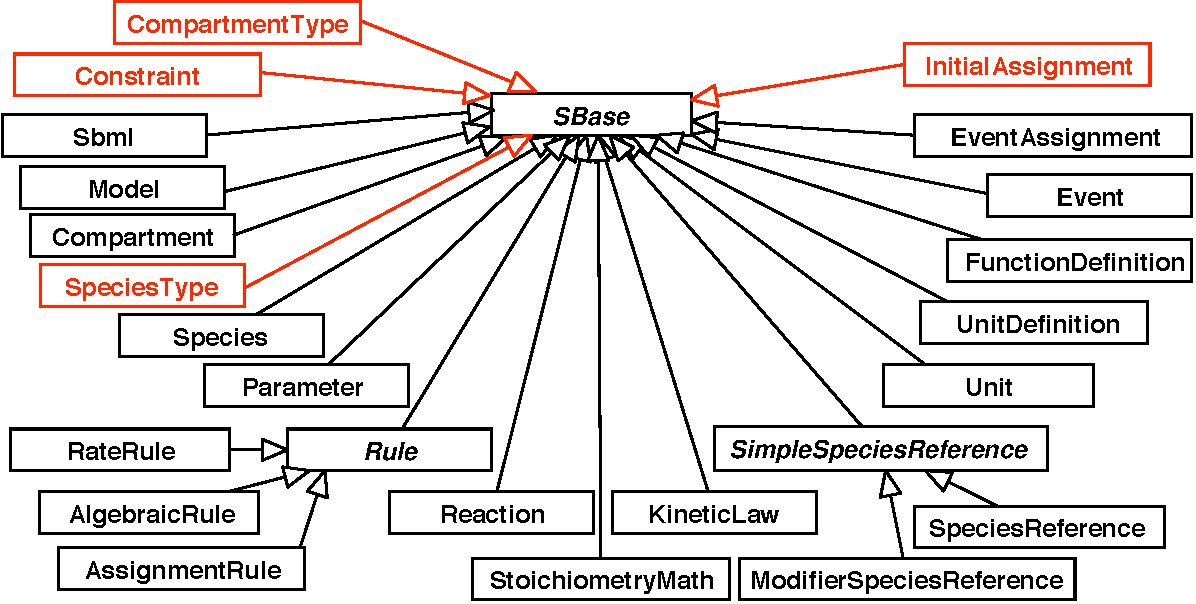
\includegraphics[scale = 0.7]{figs/top-level}
  \caption{A UML diagram of the inheritance hierarchy of major data types
    in SBML.  Open arrows indicate inheritance, pointing from inheritors to
    their parents~\protect\citep{eriksson:1998,oestereich:1999}.  In addition to
    these types, all substructures in SBML (including, for example, all the
    \token{listOf} lists) are also derived from \SBase.  See text
    for details.}
  \label{fig:top-level}
\end{figure}

\begin{blockChanged}
Although not appearing explicitly in the diagram, the various
\token{listOf\rule{0.5in}{0.5pt}} lists, as well as substructures
such as \token{trigger} on \Event (Section~\ref{sec:events}), are
also derived from \SBase.  However, substructures such as
\token{math}, containing MathML content, are not derived from
\SBase, nor are the \token{notes} and \token{annotation} fields
defined in \SBase itself (discussed in Section~\ref{sec:notes}
and~\ref{sec:annotation-use}).
\end{blockChanged}


%-----------------------------------------------------------------------------
\subsection{\changed{Type SBase}}
\label{sec:sbase}
%-----------------------------------------------------------------------------

Every structure composing an SBML Level~2 model definition has a
specific data type that is derived directly or indirectly from a
single abstract type called \SBase.  \changed{In addition to
serving as the parent class for most other classes of objects in
SBML, this} base type is designed to allow a modeler
or a software package to attach arbitrary information to each major
structure or list in an SBML model.  The definition of \SBase is
presented in Figure~\vref{fig:sbase}.

\begin{figure}[hbt]
  \centering
  \begin{classbox}{\textsl{SBase}}
    metaid: ID \{ use="optional" \}                                                                 \\
    notes: (any : \{ namespace="http://www.w3.org/1999/xhtml" \}) \{ minOccurs="0" maxOccurs="1" \} \\
    annotation: (any) \{ minOccurs="0" maxOccurs="1" \}                                             \\
  \end{classbox}
  \caption{The definition of \SBase.  Text enclosed in braces next
    to field types (e.g., \token{\{minOccurs="0"\}}) indicates
    constraints on the possible field values.  We use the XML Schema
    language to express constraints because we are primarily interested in
    the XML encoding of SBML.  The constraint expression
    \token{\{use="optional"\}} means that the indicated field is optional
    and may be omitted in a particular instance in a model.  The constraint
    expression \token{minOccurs="0"} likewise means the indicated
    field is optional; this alternate form of expression must be used for
    those fields that are containers (i.e., fields encoded as
    subelements in XML).}
  \label{fig:sbase}
\end{figure}

\SBase contains three fields, all of which are optional:
\token{metaid}, \token{notes} and \token{annotation}. These
fields are discussed separately in the following subsections.


\subsubsection{The \token{metaid} field}
\label{sec:metaid}

\begin{blockChanged}
The \token{metaid} field is present for supporting metadata
annotations using RDF~\citep[Resource Description
Format;][]{lassila:1999}.  It has a data type of XML \token{ID}
(the XML identifier type), which means each \token{metaid} value
must be globally unique within an SBML file.  The \token{metaid}
value serves to identify a model component for purposes such as
referencing that component from metadata placed within
\token{annotation} structures (see
Section~\ref{sec:annotation-use}).  Such metadata can use RDF
\token{description} elements, in which an RDF attribute called
\val{describes} contains the \token{metaid} identifier of an
object defined in the SBML model.  This topic is discussed in
greater detail in Section~\ref{sec:annotation-standard}.
\end{blockChanged}


\subsubsection{The \token{notes} field}
\label{sec:notes}

The field \token{notes} in \SBase is a container for
XHTML\changed{~1.0~\citep{pemberton:2002}} content.  It is
intended to serve as a place for storing optional information
intended to be seen by humans.  \changed{An example use of the
  \token{notes} field would be to contain formatted user comments}
about the model component in which the \token{notes} field is enclosed.
Every data object derived directly or indirectly from type \SBase
can have a separate value for \token{notes}, allowing users
considerable freedom when adding comments to their models.

\begin{blockChanged}
XHTML~1.0 is simply a formulation of HTML~4 in XML~1.0.  This
means the full power of HTML formatting is available for use in
\token{notes} content.  The intention behind requiring XHTML
(rather than, for example, plain HTML or plain text) for
\token{notes} content is to balance several conflicting goals: (1)
choosing a format for notes that is compatible with the XML form of
SBML (plain HTML would not be); (2) supporting an international
formatting standard so that users have more control over the
appearance of notes and can predict to some degree how their notes
will be displayed in different tools and environments (which
argues against using plain-text notes); and (3) achieving these
goals using an approach that is hopefully easy enough for software
developers to support using off-the-shelf programming libraries.
It is worth noting in passing that the requirement for XHTML does
not \emph{prevent} users from entering plain-text content with
simple space/tab/newline formatting: it merely requires using the
standard \token{<pre>}...\token{</pre>} element of (X)HTML.

Modern libraries for displaying and editing (X)HTML content are
commonly available in contemporary software programming
environments, and software developers may wish to avail themselves
of these facilities rather than implementing their own XHTML
support systems.


\paragraph{XML Namespace requirements for \token{notes}}

The XML content of \token{notes} elements must declare the use of
the XHTML XML namespace.  This can be done in multiple ways.  One
way is to place a namespace declaration for the appropriate
namespace URI (which is \uri{http://www.w3.org/1999/xhtml}) on the
top-level \Sbml object (see Section~\ref{sec:sbml}) and then
reference the namespace in the \token{notes} content using a
prefix.  The following example illustrates this approach:

\begin{example}
<sbml xmlns="http://www.sbml.org/sbml/level2/version2" level="2" version="2"
      xmlns:xhtml="http://www.w3.org/1999/xhtml">
  ...
  <notes>
    <xhtml:body>
      <xhtml:center><xhtml:h2>A Simple Mitotic Oscillator</xhtml:h2></xhtml:center>
      <xhtml:p>A minimal cascade model for the mitotic oscillator
      involving cyclin and cdc2 kinase</xhtml:p>
    </xhtml:body>
  </notes>
  ...
\end{example}

Another approach is to declare the XHTML namespace within the
\token{notes} content itself, as in the following example:

\begin{example}
...
<notes>
  <body xmlns="http://www.w3.org/1999/xhtml">
    <center><h2>A Simple Mitotic Oscillator</h2></center>
    <p>A minimal cascade model for the mitotic oscillator
    involving cyclin and cdc2 kinase</p>
  </body>
</notes>
...
\end{example}

The \token{xmlns="http://www.w3.org/1999/xhtml"} declaration on
\token{body} as shown above changes the default XML namespace
within it, such that all of its content is by default in the XHTML
namespace.  This is a particularly convenient approach because it
obviates the need to prefix every element with a namespace prefix
(\eg \token{xhtml:center} as in the previous case).  Other
approaches are also possible.


\paragraph{The content of \token{notes}}

SBML does not require the content of \token{notes} to be any
particular XHTML element; the content can be almost any
well-formed XHTML content.  There are only two simple
restrictions.  The first restriction comes from the requirements
of XML: the \token{notes} element must not contain an XML
declaration nor a DOCTYPE declaration.  That is, \token{notes}
must \emph{not} contain

\begin{example}
<?xml version="1.0" encoding="UTF-8"?>  
\end{example}

nor (where the following is only one specific example of a
DOCTYPE declaration)

\begin{example}
<!DOCTYPE html PUBLIC "-//W3C//DTD XHTML 1.0 Strict//EN"
 "http://www.w3.org/TR/xhtml1/DTD/xhtml1-strict.dtd">
\end{example}

% [MH] I don't think there's any way in XML to change the encoding
% in the middle of a document without using an XML declaration, is
% there?
%
%\item at no pointin the \token{notes} field can the character
%encoding be changed away from UTF-8 (the encoding for SBML);

The second restriction is intended to balance freedom of content
with the complexity of implementing software that can interpret
the content.  The content of \token{notes} in SBML can consist
only of the following possibilities:
\begin{enumerate}
  
\item A complete XHTML document (minus the XML and DOCTYPE
  declarations, of course), that is, XHTML content beginning with
  the \token{html} tag.  The following is an example skeleton:
  \begin{example}
<notes>
    <html xmlns="http://www.w3.org/1999/xhtml">
    ...
    </html>
</notes>\end{example}

\item The \token{body} element from an XHTML document.  The
  following is an example skeleton:
  \begin{example}
<notes>
    <body xmlns="http://www.w3.org/1999/xhtml">
    ...
    </body>
</notes>\end{example}
  
\item Any XHTML content that would be permitted within a
  \token{body} element.  Note that if this consists of multiple
  elements, each one must declare the XML namespace separately.
  The following is an example skeleton example:
  \begin{example}
<notes>
    <p xmlns="http://www.w3.org/1999/xhtml">
    ...
    </p>
    <p xmlns="http://www.w3.org/1999/xhtml">
    ...
    </p>
</notes>\end{example}

\end{enumerate}
Another way to summarize the restrictions above is simply to say
that the content of an SBML \token{notes} element can be only be a
complete \token{html} element, a \token{body} element, or whatever
is permitted inside a \token{body} element.  In practice, this
does not limit in any meaningful way what can be placed inside a
\token{notes} element; for example, if an application or modeler
wants to put a complete XHTML page, including a \token{head}
element, it can be done by putting in everything starting with the
\token{html} container.  However, the restrictions above do make
it somewhat simpler to write software that can read and write the
\token{notes} content.  Appendix~\ref{apdx:processing-notes}
describes one possible approach to doing just that.

\end{blockChanged}


\begin{blockChanged}
\subsubsection{The \token{annotation} field}
\label{sec:annotation-use}

Whereas the \token{notes} field described above is a container for
content to be shown directly to humans, the \token{annotation}
field is a container for optional software-generated content
\emph{not} meant to be shown to humans.  Every data object derived
from \SBase can have its own value for \token{annotation}.  The
field's data type is XML type \token{any}, allowing essentially
arbitrary data content.  SBML places only a few restrictions on
the organization of the content; these are intended to help
software tools read and write the data as well as help reduce
conflicts between annotations added by different tools.


\paragraph{The use of XML Namespaces in \token{annotation}}

% FIXME 2006-03-19:
% we should mention that RDF is an additional thing that can show
% up in annotations.  basically what's happening here is that we're
% saying any/all rdf content must be lumped together in one place

At the outset, software developers should keep in mind that multiple
software tools may attempt to read and write annotation content.  To reduce
the potential for collisions between annotations written by different
applications, \sbmltwotwo stipulates that tools must use XML
namespaces~\citep{bray:1999} to specify the intended vocabulary of every
annotation.  The application's developers must choose a URI
(\emph{Universal Resource Identifier}; \citealt{harold:2001,w3c:2000})
reference that uniquely identifies the vocabulary the application will use,
and a prefix string for the annotations.  Here is an example.  Suppose an
application uses the URI \uri{http://www.mysim.org/ns} and the
prefix \token{mysim} when writing annotations related to screen layout.
The content of an annotation might look like the following:

\begin{example}
<annotation>
    <mysim:nodecolors xmlns:mysim="http://www.mysim.org/ns"
         mysim:bgcolor="green"
         mysim:fgcolor="white"/>
</annotation>
\end{example}

In this particularly simple case, the content consists of a single XML
element (\token{nodecolors}) with two attributes (\token{bgcolor},
\token{fgcolor}), all of which are prefixed by the string \token{mysim}.
(Presumably this particular content would have meaning to the hypothetical
application in question.)  The content in this particular example is small,
but it should be clear that there could easily have been an arbitrarily large
amount of data placed inside the \token{mysim:nodecolors} element.

The key point of the example above is that application-specific annotation data
is entirely contained inside a single \emph{top-level element} within the
SBML \token{annotation} container.  \sbmltwotwo places the following
restrictions on annotations:
\begin{itemize}

\item Within a given SBML \token{annotation} element, there can
  only be one top-level element using a given namespace.  An
  annotation element can contain multiple top-level elements but
  each must be in a different namespace.

\item No top-level element in an \token{annotation} may use an
  SBML XML namespace, either explicitly by referencing one of the
  SBML XML namespace URIs or implicitly by failing to specify any
  namespace on the annotation.  (As of \sbmltwotwo, the defined
  SBML namespaces are the following URIs:
  \uri{http://www.sbml.org/sbml/level1},
  \uri{http://www.sbml.org/sbml/level2}, as well as
  \uri{http://www.sbml.org/sbml/level2/version2}.)

\item The ordering of top-level elements within a given
  \token{annotation} element is \emph{not} significant.  An
  application should not expect that its annotation content
  appears first in the \token{annotation} element, nor in any
  other particular location.

\end{itemize}

The use of XML namespaces in this manner is intended to improve the ability
of multiple applications to place annotations on SBML model structures with
reduced risks of interference or name collisions.  Annotations stored by
different simulation packages can therefore coexist in the same model
definition.  The rules governing the content of \token{annotation} elements
are designed to enable applications to easily add, change, and remove their
annotations from SBML elements while simultaneously preserving annotations
inserted by other applications when mapping SBML from input to output.

Some more examples hopefully will make this more clear.  The next
example is invalid because it contains a top-level element in the
SBML XML namespace---this happens because no namespace is declared
for the \token{<cytoplasm>} element, which means by default it
falls into the SBML namespace:

\begin{example}
<annotation>
    <cytoplasm/>
</annotation>
\end{example}

The following example is invalid because it contains two top-level
elements using the same XML namespace.  Note that it does not
matter that these are two different top-level elements
(\token{<nodecolors>} and \token{<textcolors>}); what matters is
that these separate elements are both in the same namespace rather
than having been collected and placed inside one overall container
element for that namespace.

\begin{example}
<annotation>
    <mysim:nodecolors xmlns:mysim="http://www.mysim.org/ns"
        mysim:bgcolor="green"
        mysim:fgcolor="white"/>
    <mysim:textcolors xmlns:mysim="http://www.mysim.org/ns"
        mysim:bgcolor="green"
        mysim:fgcolor="white"/>
</annotation>
\end{example}

On the other hand, the following example is valid:

\begin{example}
<annotation>
    <mysim:geometry xmlns:mysim="http://www.mysim.org/ns"
         mysim:bgcolor="green" mysim:fgcolor="white">
        <graph:node xmlns:graph="http://www.graph.org/ns" graph:x="4" graph:y="5" />
    </mysim:geometry>
    <othersim:icon xmlns:othersim="http://www.othersim.com/">
        WS2002
    </othersim:icon>
</annotation>
\end{example}

It is worth keeping in mind that although XML namespace names must
be URIs, they are (like all XML namespace names) \emph{not
required} to be directly usable in the sense of identifying an
actual, retrieval document or resource on the
Internet~\citep{bray:1999}.  URIs such as
\uri{http://www.mysim.org/} may appear as though they are (\eg)
Internet addresses, but there are not the same thing.  This style
of URI strings, using a domain name and other parts, is only a
simple and commonly-used way of creating a unique name string.

Finally, note that the namespaces being referred to here are XML
namespaces specifically in the context of the \token{annotation}
field on \SBase.  The namespace issue here is unrelated to the
namespaces discussed in \changed{Section~\ref{sec:identifiers} in the
context of component identifiers in SBML.}


\paragraph{Content of annotations and implications for software tools}

The \token{annotation} field in the definition of \SBase
exists in order that software developers may attach optional
application-specific data to the structures in an SBML model. However,
it is important that this facility not be misused.  In particular,
it is \emph{critical} that data essential to a model definition
\changed{or that can be encoded in existing SBML
structures} is \emph{not} stored in \token{annotation}. Parameter
values, functional dependencies between model structures, etc.,
should not be recorded as annotations.  It is crucial to keep in
mind the fact that data placed in annotations can be freely ignored by
software applications.  If such data affects the interpretation
of a model, then software interoperability is greatly impeded.

Here are examples of the kinds of data that may be appropriately
stored in \token{annotation}: (a) information about the graphical
layout of model components; (b) application-specific processing
instructions that do not change the essential meaning of a model;
(c) identification information for cross-referencing components in
a model with items in a data resource such as a database.

\paragraph{Standardized format for certain classes of annotations}

For case (c) above (i.e., information for cross-referencing components in a
model to data resources), \sbmltwotwo recommends a standard format for use
within an \token{annotation} field.  This format should be used in
preference to proprietary syntaxes to maximize the likelihood that multiple
software tools will converge on the same syntax for this kind of
information.  The \sbmltwotwo recommended scheme is described in
Section~\ref{sec:finney-novere}.

\end{blockChanged}


%-----------------------------------------------------------------------------
\subsection{The \token{id} and \token{name} fields on SBML components}
\label{sec:idnameattribs}
%-----------------------------------------------------------------------------

\begin{blockChanged}

As will become apparent below, most structures in SBML include two
common fields: \token{id} and \token{name}.  These fields are not
defined on \SBase (as explained in
Section~\ref{sec:why-not-on-sbase} below), but where they do
appear, the common rules of usage described below apply.


\subsubsection{The \token{id} field and identifier scoping}
\label{sec:identifiers}

The \token{id} field is a mandatory field on most structures in
SBML.  It is used to identify a component within the model
definition.  Other SBML structures can refer to the component
using this identifier.  The data type of \token{id} is always
either \primtype{Sid} (Section~\ref{sec:sid}) or
\primtype{UnitSId} (Section~\ref{sec:unitsid}), depending on the
object in question.

\end{blockChanged}

A model can contain a large number of components representing
different parts.  This leads to a problem in deciding the scope of
an identifier: in what contexts does a given identifier \emph{X}
represent the same thing?  The approaches used in existing
simulation packages tend to fall into two categories which we may
call global and local.  The \emph{global} approach places all
identifiers into a single global space of identifiers, so that an
identifier \emph{X} represents the same thing wherever it appears
in a given model definition.  The \emph{local} approach places
symbols in separate identifier namespaces, depending on the
context, where the context may be, for example, individual
reaction rate expressions.  The latter approach means that a user
may use the same identifier \emph{X} in different rate expressions
and have each instance represent a different quantity.

The fact that different simulation programs may use different
rules for identifier resolution poses a problem for the exchange
of models between simulation tools.  Without careful
consideration, a model written out in SBML format by one program
may be misinterpreted by another program.  \sbmltwo must
therefore include a specific set of rules for treating identifiers
and \changed{their scopes}.

The \changed{scoping} rules in \sbmltwo are relatively
straightforward and are intended to avoid this problem with a
minimum of requirements on the implementation of software tools:
\begin{itemize}
  
\item \changed{The identifier (\ie the values of the field
    \token{id}) of every \FunctionDefinition, \CompartmentType,
    \SpeciesType, \Compartment, \Species, \Parameter, \Reaction,
    \SpeciesReference, \ModifierSpeciesReference, \Event, and
    \Model, must be unique across the set of all such identifiers
    in the model.  This means, for example, that a reaction and a
    species definition cannot both have the same identifier.}

\item \changed{The identifier of every \UnitDefinition must be
    unique across the set of all such identifiers in the model;
    however, unit identifiers live in a separate space of
    identifiers from other identifiers in the model.}
  
\item Each \changed{\Reaction instance} (see
  Section~\ref{sec:reactions}) establishes a separate private
  local space for local \Parameter identifiers.  \changed{Within
    the definition of that reaction, local parameter identifiers
    override (shadow) identical identifiers outside of that
    reaction.  Of course, the corollary of this is that local
    parameters inside a \Reaction object instance are not visible
    to other objects outside of that reaction.}

\end{itemize}
The set of rules above can enable software packages using either
local or global identifier spaces for parameters to exchange SBML
model definitions.  \changed{Software systems} using local
identifiers for parameters internally should, in principle, be
able to accept SBML model definitions without needing to change
component identifiers.  Environments using a common global space
of identifiers for parameters internally can perform manipulations
of the identifiers of local parameters within reaction definitions
to avoid \changed{identifier} collisions.

% [2006-04-01 AF] Removed the following because a its not >that< simple and
% the the approach you outline is not bullet proof and I don't
% think its a good idea to create a hostage to fortune for
% naive implementors.  In practice you have to (a) ensure the
% generated ids use a seperator (e.g. '.') that contains one or more characters
% that are not valid sbml id characters (to eliminate other namespace collisions)
% (this assumes you never write out the transformed model as SBML!!)
% (b) substitute the new ids into the kinetic law (c) add the new ids to the
% global parameter list.
%
%(An example approach for
%the latter would be the following: when receiving an SBML-encoded
%model, prefix each parameter identifier inside each reaction with
%a string constructed from the reaction's identifier; when writing
%an SBML-encoded model, strip off the prefix.)

The guidelines described here will hopefully provide a clean
transition path to future levels of SBML, when submodels are
introduced (Section~\ref{sec:level-3}).  Submodels will provide
the ability to compose one model from a collection of other
models.  This capability will have to be built on top of
\sbmltwo's namespace organization.  A straightforward approach to
handling namespaces is to make each submodel's space be private.
The rules governing identifier scoping within a submodel can
simply be the Level~2 namespace rule described here, with each
submodel having its own (to itself, global) namespace.


\subsubsection{The \token{name} field}
\label{sec:name}

In contrast to the \token{id} field, the \token{name} field is
optional and is not intended to be used for cross-referencing
purposes within a model.  Its purpose instead is to provide a
human-readable label for the component.  The data type of the
\token{name} field is the type \primtype{string} defined in XML
Schema~\citep{biron:2000,thompson:2000} and discussed further in
Section~\ref{sec:primitive-types}.  SBML imposes no restrictions
as to the content of \token{name} fields beyond those restrictions
defined by the \primtype{string} type in XML Schema.

The recommended practice for handling \token{name} is as follows.
If a software tool has the capability for displaying the content
of \token{name} fields, it should display this content to the user
as a component's label instead of the component's \token{id}
field.  If the user interface does not have this capability (e.g.,
because it cannot display or use special characters in symbol
names), or if the \token{name} field is missing on a given
component, then the user interface should display the value of the
\token{id} field instead.  (Script language interpreters are
especially likely to display \token{id} fields instead of
\token{name} fields.)

As a consequence of the above, authors of systems that
automatically generate the values of \token{id} fields should be
aware some systems may display the \token{id}'s to the user.
Authors therefore may wish to take some care to have their
software create \token{id} values that are: (a) reasonably easy
for humans to type and read; and (b) likely to be meaningful, \eg
the id field is an abbreviated form of the name field value.

\begin{blockChanged}
An additional point worth mentioning is although there are
restrictions on the uniqueness of \token{id} values (see
Section~\ref{sec:identifiers} above), there are no restrictions on
the uniqueness of \token{name} values in a model.  This allows
software packages leeway in assigning component identifiers.
\end{blockChanged}

%For example, a species in an SBML model must be
%located in a compartment, which means that if the same species appears in
%multiple compartments (e.g., in the context of a transport reaction), they
%must be given different identifiers.  It is currently the case that users
%and software differ sharply in philosophy about how to treat this
%situation: some treat these as different species, and others treat them as
%the same species located in different places.  Those in the latter group
%often want to use the same \token{name} but have different \token{id}
%values for the differently-localized ``instances'' of the species.  The
%freedom from restrictions on \token{name} values enables SBML to
%accommodate both philosophies.


\begin{blockChanged}

\subsubsection{Why \token{id} and \token{name} are not defined on \class{SBase}}
\label{sec:why-not-on-sbase}

% [MH 2006-03-06] Most of the following issues could be addressed
% by having a separate "SBaseWithId" class.  I think only the first
% two reasons couldn't be addressed.  Thus, the original paragraph
% (which only talked about scoping) was almost in some sense the
% fundamental reason.  I added this other stuff to address some
% questions made in the past, but these other arguments are all
% trumped by saying ``just define an SBaseWithID''.  Therefore,
% it may be worth thinking about going back to the single reason.

Although many SBML components also feature two other fields named
\token{id} and \token{name}, these fields are purposefully not defined on
\SBase.  There are several reasons for this.
\begin{itemize}
  
\item The presence of an SBML identifier field (\token{id})
  necessarily requires specifying scoping rules for the
  corresponding identifiers.  However, the \SBase abstract type is
  used as the basis for defining components whose scoping rules
  are in some cases different from each other.  (See
  Section~\ref{sec:identifiers} for more details).  If \SBase were
  to have an \token{id} field, then the specification of \SBase
  would need a default scoping rule and this would then have to be
  overloaded on derived classes that needed different scoping.
  This would make the SBML specification more complex.
  
\item Identifier are optional on some SBML components and required
  on most others.  If \token{id} were defined as optional on
  \SBase, most component classes would separately have to redefine
  \token{id} as being mandatory---hardly an improvement over the
  current arrangement.  Conversely, if \token{id} were defined as
  mandatory on \SBase, it would prevent it from being optional on
  components where it \emph{is} currently optional.
  
\item The \SBase abstract type is used as the base type for
  certain structures such as \Sbml, \Unit, \AssignmentRule, etc.,
  which do not have identifiers because these structures do not
  need to be referenced by other structures.  If \SBase had a
  mandatory \token{id} field, \emph{all} objects of these other
  types in a model would then need to be assigned unique
  identifiers.  Similarly, because \SBase is the base type of the
  \token{listOf\rule{0.5in}{0.5pt}} lists (see
  Section~\ref{sec:type-inheritance-hierarchy}), putting
  \token{id} on \SBase would require all of these lists in a model
  to be given identifiers.  This would be a needless burden on
  software developers, tools, and SBML users, requiring them to
  generate and store additional identifiers for objects that never
  need them.
  
\item \SBase does not have a \token{name} simply because such a
  field is always paired with an \token{id} field.  Without
  \token{id} on \SBase, it does not make sense to have
  \token{name}.

\end{itemize}

\end{blockChanged}


%-----------------------------------------------------------------------------
\subsection{Mathematical formulas in SBML Level 2}
\label{sec:formulas}
%-----------------------------------------------------------------------------

% I no longer understand why we need to bother with this long list
% here.  It only seems to make it harder to read.  There's no
% value added, in my mind, so I'm commenting it out. [2006-09-06 MH]
%
%It is used in the
%definitions of functions (Section~\ref{sec:functiondefinition}), rules
%(Section~\ref{sec:rules}), initial assignments
%(Section~\ref{sec:initialAssignment}), constraints
%(Section~\ref{sec:constraints}), reaction kinetics
%(Section~\ref{subsec:kinetic-law}), stoichiometries
%(Section~\ref{subsec:speciesreference}) and events
%(Section~\ref{sec:events}). The \FunctionDefinition, \KineticLaw,
%\StoichiometryMath, \EventAssignment,
%\changed{\InitialAssignment, \Constraint}, and
%\Rule structures each have a single MathML \token{math}
%subelement.  \changed{The \Event structure has two \token{math} elements, one
%inside a subelement named \token{trigger} and the other inside
%a subelement named \token{delay}.  The \FunctionDefinition's single
%\token{math} element is limited to containing only a single MathML
%\token{lambda} element.}

\begin{blockChanged}
Mathematical expressions in SBML Level~2 are represented using
\mathmltwo~\citep{w3c:2000b}.  MathML is an international standard
for encoding mathematical expressions using XML.  There are two
principal facets of MathML, one for encoding content (\ie the
semantic interpretation of a mathematical expression), and another
for encoding presentation or display characteristics.  SBML only
makes direct use of a subset of the content portion of MathML.  
By borrowing a separately-developed XML standard, we can avoid
having to define a specialized syntax for mathematical expressions
in SBML and simultaneously leverage existing intellectual and
technological work already done in the MathML community.  However,
it is not possible to produce a completely smooth and conflict-free
interface between MathML and other standards used by SBML (in
particular, \xmlschema).  Two specific issues and their
resolutions are discussed in Sections~\ref{sec:cn-token}.

The XML namespace URI for all MathML elements is
\uri{http://www.w3.org/1998/Math/MathML}.  Everywhere MathML
content is allowed in SBML, the MathML elements must be properly
placed within the \mathmltwo namespace.  In XML, this can be
accomplished in a number of ways, and the examples throughout this
specification illustrate the use of this namespace and MathML in
SBML.  Please refer to the W3C document by \citet{bray:1999} for
more technical information about using XML namespaces.
\end{blockChanged}


\subsubsection{Subset of MathML used in SBML Level 2}
\label{sec:mathmlsubset}

The subset of \mathmltwo elements used in SBML Level~2 is similar to
that used by CellML~\changed{\citep{hedley:2001b}, another model
definition language with similar goals as SBML.  The subset of MathML
elements used in SBML is listed below:}
\begin{itemize}\setlength{\parskip}{-0.2ex}

\item \emph{token}: \token{cn}, \token{ci}, \token{csymbol},
  \token{sep}
  
\item \emph{general}: \token{apply}, \token{piecewise},
  \token{piece}, \token{otherwise}, \token{lambda} (the last is
  restricted to use in \FunctionDefinition)

\item \emph{relational operators}: \token{eq}, \token{neq},
  \token{gt}, \token{lt}, \token{geq}, \token{leq}

\item \emph{arithmetic operators}: \token{plus}, \token{minus},
  \token{times}, \token{divide}, \token{power}, \token{root},
  \token{abs}, \token{exp}, \token{ln}, \token{log},
  \token{floor}, \token{ceiling}, \token{factorial}

\item \emph{logical operators}: \token{and}, \token{or},
  \token{xor}, \token{not}

\item \emph{qualifiers}: \token{degree}, \token{bvar},
  \token{logbase}

\item \emph{trigonometric operators}: \token{sin}, \token{cos},
  \token{tan}, \token{sec}, \token{csc}, \token{cot},
  \token{sinh}, \token{cosh}, \token{tanh}, \token{sech},
  \token{csch}, \token{coth}, \token{arcsin}, \token{arccos},
  \token{arctan}, \token{arcsec}, \token{arccsc}, \token{arccot},
  \token{arcsinh}, \token{arccosh}, \token{arctanh},
  \token{arcsech}, \token{arccsch}, \token{arccoth}

\item \emph{constants}: \token{true}, \token{false},
  \token{notanumber}, \token{pi}, \token{infinity},
  \token{exponentiale}

\item \emph{annotation}: \token{semantics}, \token{annotation},
  \token{annotation-xml}

\end{itemize}
\vspace*{-0.75ex}
The inclusion of logical operators, relational operators,
\token{piecewise}, \token{piece}, and \token{otherwise} elements
facilitates the encoding of discontinuous expressions.
\changed{Note that MathML} elements for representing partial
differential calculus are not included.  We anticipate that the
requirements for partial differential calculus will be addressed
in proposals for future SBML geometry representations (see
Section~\ref{sec:level-3}).

\changed{As defined by \mathmltwo, the semantic interpretation of
the mathematical functions listed above follows the definitions
of the functions laid out by \cite{abramowitz:1997} and
\cite{zwillinger:1988}.  Readers are directed to these sources
and the MathML specification for information about such things
as which principle values of the inverse trigonometric functions
to use.}

\changed{Software authors should take particular note of the
MathML semantics of the N-ary operators \token{plus},
\token{times}, \token{and}, \token{or} and \token{xor}, when
they are used with different numbers of arguments.  The MathML
specification~\citep{w3c:2000b} appendix C.2.3 describes the
semantics for these operators with zero, one, and more
arguments.}

The following are the only attributes permitted on MathML elements
in SBML (in addition to the \token{xmlns} attribute on
\token{math} elements):
\begin{itemize}\setlength{\parskip}{-0.2ex}

\item \token{style}, \token{class} and \token{id} on any element;

\item \token{encoding} and \token{definitionURL} on
  \token{csymbol} elements; and

\item \token{type} on \token{cn} elements.

\end{itemize}\vspace*{-0.75ex}
Missing values for these attributes are to be treated in the same
way as defined by MathML.  These restrictions on attributes are
designed to confine the MathML elements to their default semantics
and to avoid conflicts in the interpretation of the type of token
elements.


\begin{blockChanged}
\subsubsection{Numbers and \token{cn} elements}
\label{sec:cn-token}
\label{sec:mathml-value-space}

In MathML, literal numbers are written as the content portion of a
particular element called \token{cn}.  This element takes an
optional attribute, \token{type}, used to indicate the \emph{type}
of the number (such as whether it is meant to be an integer or a
floating-point quantity).  Here is an example of its use:
\begin{example}
<math xmlns="http://www.w3.org/1998/Math/MathML">
    <apply>
        <times/> <cn type="integer"> 42 </cn> <cn type="real"> 3.3 </cn>
    </apply>
</math>
\end{example}

The content of a \token{cn} element must be a number.  The number
can be preceded and succeeded by whitespace (see
Section~\ref{sec:mathml-whitespace}).  The following are the only
permissible values for the \token{type} attribute on MathML
\token{cn} elements: \val{e-notation}, \val{real}, \val{integer},
and \val{rational}.  The value of the \token{type} attribute
defaults to \val{real} if it is not specified on a given
\token{cn} element.


\paragraph{Value space restrictions on \token{cn} content}

SBML imposes certain restrictions on the value space of numbers
allowed in MathML expressions.  According to the \mathmltwo
specification, the values of the content of \token{cn} elements do
not necessarily have to conform to any specific floating point or
integer representations designed for CPU implementation.  For
example, in strict MathML, the value of a \token{cn} element could
exceed the maximum value that can be stored in a IEEE 64 bit
floating point number (IEEE 754).  This is different from the XML
Schema type \primtype{double} that is used in the definition of
floating point fields of structures in SBML; the XML Schema
\primtype{double} \emph{is} restricted to IEEE double-precision
64-bit floating point type IEEE 754-1985.  To avoid an
inconsistency that would result between numbers elsewhere in SBML
and numbers in MathML expressions, \sbmltwotwo imposes the
following restriction on MathML content appearing in SBML:
\begin{itemize}
  
\item Integer values (\ie the content of \token{cn} elements
  having \token{type}=\val{integer}) must conform to the
  \primtype{int} type used elsewhere in SBML
  (Section~\ref{sec:integer})
  
\item Floating-point values (\ie the content of \token{cn}
  elements having \token{type}=\val{real} or
  \token{type}=\val{e-notation}) must conform to the
  \primtype{double} type used elsewhere in SBML
  (Section~\ref{sec:double})
\end{itemize}


\paragraph{Syntactic differences in the representation of numbers
  in scientific notation}

It is important to note that MathML uses a style of scientific
notation that differs from what is defined in XML Schema, and
consequently what is used in SBML attribute values.  The
\mathmltwo type \val{e-notation} requires the mantissa and
exponent to be separated by one \texttt{<sep/>} element.  The
mantissa must be a real number and the exponent part must be a
signed integer.  This leads to expressions such as

\begin{example}
<cn type="e-notation"> 2 <sep/> -5 </cn>
\end{example}

for the number $2 \times 10^{-5}$.  It is especially
important to note that the expression

\begin{example}
<cn type="e-notation"> 2e-5 </cn>
\end{example}

is \emph{not valid} in \mathmltwo and therefore cannot be used in
MathML content in SBML.  However, elsewhere in SBML, when an
attribute value is declared to have the data type
\primtype{double} (a type taken from XML Schema), the compact
notation \val{2e-5} is in fact allowed.  In other words, within
MathML expressions contained in SBML (and \emph{only} within such
MathML expressions), numbers in scientific notation must take the
form \token{<cn type="e-notation"> 2 <sep/> -5 </cn>}, and
everywhere else they must take the form \val{2e-5}.

This is a regrettable difference between two standards that SBML
replies upon, but it is not feasible to redefine these types
within SBML because the result would be incompatible with parser
libraries written to conform with the MathML and XML Schema
standards.  It is also not possible to use XML Schema to define a
data type for SBML attribute values permitting the use of the
\token{<sep/>} notation, because XML attribute values cannot
contain XML elements---that is, \token{<sep/>} cannot appear in an
XML attribute value.

\end{blockChanged}


\subsubsection{Use of \token{ci} elements in MathML expressions in SBML}
\label{sec:ci-token}

\changed{The content of a \token{ci} element must be an SBML identifier
that is declared elsewhere in the model.  The identifier can be
preceded and succeeded by whitespace.} The set of possible
identifiers that can appear in a \token{ci} element depends on the
containing structure in which the \token{ci} is used:
\begin{itemize}
  
\item If a \token{ci} element appears in the body of \changed{a
  \FunctionDefinition object
  (Section~\ref{sec:functiondefinition})}, the referenced
  identifier must be either (i) one of the declared arguments to
  that function, or (ii) the identifier of a previously defined
  \changed{\FunctionDefinition object} in the model.
  
\item \changed{Otherwise, the referenced identifier must be that
    of a \Species, \Compartment, \Parameter, \FunctionDefinition,
    or \Reaction object defined in the model.}  The following are
  the only possible interpretations of using such an identifier in
  SBML:
  \begin{itemize}
    
  \item \emph{Species identifier}: When a \changed{\Species}
    identifier occurs in a \token{ci} element, it represents the
    quantity \changed{of that species in terms of either
      \quantity{amount of substance} units or in terms of
      \quantity{concentration} units, depending on the definition
      of that species; see Section~\ref{sec:species-units}.}
    
  \item \emph{Compartment identifier}: When a
    \changed{\Compartment} identifier occurs in a \token{ci}
    element, it represents the size of the compartment.  The units
    associated with the size of the compartment are those given on
    the \Compartment structure that declares the identifier; see
    Section~\ref{sec:compartment-units}.
    
  \item \emph{Parameter identifier}: When a \changed{\Parameter}
    identifier occurs in a \token{ci} element, it represents the
    \changed{numerical} value assigned to that parameter.  The
    units associated with the parameter's value are the units
    assigned in its instance of a \Parameter structure; see
    Section~\ref{sec:parameter-units}.
    
  \item \emph{Function identifier}: When a
    \changed{\FunctionDefinition} identifier occurs in a
    \token{ci} element, it represents a call to that function.
    Function references in MathML occur in the context of using
    MathML's \token{apply} and often involve supplying arguments
    to the function; see Section~\ref{sec:functiondefinition}.
    
  \item \changed{\emph{Reaction identifier}: When a \Reaction
      identifier occurs in a \token{ci} element, it represents the
      rate of that reaction as determined by the mathematical
      formula in the \KineticLaw object within the \Reaction.  The
      units associated with the reaction are
      \quantity{substance}/\quantity{time}, with the
      \quantity{substance} and \quantity{time} units established
      by the values of the SBML built-in units \val{substance} and
      \val{time}, respectively.  These units may be redefined in
      model; see Section~\ref{sec:built-in-units}.  If the
      reaction definition has no \KineticLaw, the use of the
      reaction identifier is an error (perhaps indicating that the
      model is incomplete).}

  \end{itemize}

\end{itemize}

\begin{blockChanged}
The content of \token{ci} elements in MathML formulas outside of a
\KineticLaw or \FunctionDefinition must always refer to objects
declared in the top level global namespace; \ie SBML uses ``early
binding'' semantics.  Inside of \KineticLaw, a \token{ci} element
can additionally refer to local parameters defined within that
\KineticLaw instance; see Section~\ref{subsec:kinetic-law} for
more information.
\end{blockChanged}


\subsubsection{\changed{Handling of whitespace}}
\label{sec:mathml-whitespace}

\begin{blockChanged}
\mathmltwo defines ``whitespace'' in the same way as XML does, \ie
the space character (Unicode hexadecimal code 0020), horizontal
tab (code 0009), newline or line feed (code 000A), and carriage
return (code 000D).  In MathML, the content of elements such as
\token{cn} and \token{ci} can be surrounded by whitespace
characters.  Prior to using the content, this whitespace is
``trimmed'' from both ends: all whitespace at the beginning and
end of the content is removed~\citep{ausbrooks:2003}.  For
example, in \texttt{<cn> 42 </cn>}, the amount of white space on
either side of the ``\texttt{42}'' inside the \texttt{<cn>}
\ldots\ \texttt{</cn>} container does not matter.  Prior to
interpreting the content, the whitespace is removed altogether.
\end{blockChanged}



\subsubsection{Use of \token{csymbol} elements in MathML expressions in SBML}
\label{sec:csymbol-token}

SBML Level 2 uses the MathML \token{csymbol} element to denote
certain built-in mathematical entities without introducing
reserved names into the component identifier namespace.  The
\token{encoding} field of \token{csymbol} should be set to
\val{text}.  The \token{definitionURL} should be set to one of the
following predefined SBML symbol URIs:
\begin{itemize}

\item \uri{http://www.sbml.org/sbml/symbols/time}.  This
  represents the current simulation time.  \changed{See
  Section~\ref{sec:meaning-of-time} for more information.}  The
  units of the current time entity are determined from the
  built-in \token{time} of Table~\vref{tab:builtin}.

\item \uri{http://www.sbml.org/sbml/symbols/delay}.  This
  represents a delay function.  The delay function has the form
  $delay(x, d)$, taking two \changed{MathML expressions as}
  arguments.  Its value is the value of argument $x$ at $d$ time
  units before the current time.  \changed{There are no
    restrictions on the form of $x$.} The units of the $d$
  parameter are determined from the built-in \token{time}.
  \changed{The value of the $d$ parameter, when evaluated, must be
    numerical and be greater than or equal to 0.}  The
  \emph{delay} function is useful for representing biological
  processes having a delayed response, but where the detail of the
  processes and delay mechanism is not relevant to the operation
  of a given model.  \changed{See
    Section~\ref{sec:meaning-of-time} below for additional
    considerations surrounding the use of this \token{csymbol}.}

\end{itemize}

The following examples demonstrate these concepts.  The XML fragment below
encodes the formula $x + t$, where $t$ stands for time.

\begin{example}
<math xmlns="http://www.w3.org/1998/Math/MathML">
    <apply>
        <plus/>
        <ci> x </ci>
        <csymbol encoding="text" definitionURL="http://www.sbml.org/sbml/symbols/time">
            t
        </csymbol>
    </apply>
</math>
\end{example}

\begin{blockChanged}
In the fragment above, the use of the token \token{t} is mostly a
convenience for human readers---the string inside the
\token{csymbol} could have been almost anything, because it is
essentially ignored by MathML parsers and SBML.  Some MathML and
SBML processors will take note of the token and use it when
presenting the mathematical formula to users, but the token used
has no impact on the interpretation of the model and it does
\emph{not} enter into the SBML component identifier namespace.  In
other words, the SBML model cannot refer to \token{t} in the
example above.  The content of the \token{csymbol} element is for
rendering purposes only and can be ignored by the parser.
\end{blockChanged}

As a further example, the following XML fragment encodes the equation
$k + delay(x, 0.1)$ or alternatively $k_t + x_{t - 0.1}$:

\begin{example}
<math xmlns="http://www.w3.org/1998/Math/MathML">
    <apply>
        <plus/>
        <ci> k </ci>
        <apply>
            <csymbol encoding="text" definitionURL="http://www.sbml.org/sbml/symbols/delay">
                delay
            </csymbol>
            <ci> x </ci>
            <cn> 0.1 </cn>
        </apply>
    </apply>
</math>
\end{example}

Note that the URI in the value of \token{definitionURL}, as all
URIs, is intended to serve as a unique identifier and is not
intended to be dereferenced as an Internet address.  There is
nothing actually located at the address
\uri{http://www.sbml.org/sbml/symbols/delay}.


\begin{blockChanged}
\subsubsection{Simulation time}
\label{sec:meaning-of-time}

The principal use of SBML is to represent quantitative dynamical
models whose behaviors manifest themselves over time.  In defining
an SBML model using constructs such as reactions, time is most
often implicit and does not need to be referred to in the
mathematical expressions themselves.  However, sometimes an
explicit time dependency needs to be stated, and for this purpose,
the \emph{time} \token{csymbol} (described above in
Section~\ref{sec:csymbol-token}) may be used.  This \emph{time}
symbol refers to ``instantaneous current time'' in a simulation,
frequently given the literal name $t$ in one's equations.

An assumption in SBML is that ``start time'' or ``initial time''
in a simulation is zero, that is, if $t_0$ is the initial time in
the system, $t_0 = 0$.  This corresponds to the most common
scenario.  Initial conditions in SBML take effect at time $t = 0$.
There is no mechanism in SBML for setting the initial time to a
value other than 0.  To refer to a different time in a model, one
approach is to define a \Parameter for a new time variable and
use an \AssignmentRule in which the assignment expression
subtracts a value from the \token{csymbol} \emph{time}.  For
example, if the desired offset is 2 time units, the MathML
expression would be

\begin{example}
<math xmlns="http://www.w3.org/1998/Math/MathML">
    <apply>
        <minus/>
        <csymbol encoding="text" definitionURL="http://www.sbml.org/sbml/symbols/time"> t
        </csymbol>
        <cn> 2 </cn>
    </apply>
</math>
\end{example}

SBML's assignment rules (Section~\ref{sec:assignmentrule}) can be
used to express mathematical statements that hold true at all
moments, so using an assignment rule with the expression above
will result in the value being equal to $t - 2$ at every point in
time.  A parameter assigned this value could then be used
elsewhere in the model, its value could be plotted by a simulator,
etc.


\subsubsection{Initial conditions and special considerations}
\label{sec:before-t0}

%Although SBML does not define the simulation or other algorithms
%that may be applied to a model, the SBML specification must define
%a consistent interpretation of the various possible constructs in
%a model.  

The identifiers of \Species, \Compartment, \Parameter, and
\Reaction object instances in a given SBML model refer to the main
variables in a model.  Depending on certain attributes of these
objects (\eg the \token{constant} flag on species, compartments
and parameters---this and other conditions are explained in the
relevant sections elsewhere in this document), some of the
variables may have constant values throughout a simulation, and
others' values may change.  These changes in values over time are
determined by the system of equations constructed from the model's
reactions, initial assignments, rules, and events.

As described in Section~\ref{sec:meaning-of-time}, an SBML model's
simulation is assumed to begin at $t = 0$.  The availability of
the \emph{delay} \token{csymbol} (Section~\ref{sec:csymbol-token})
introduces the possibility that at $t = 0$, mathematical
expressions in a model may draw on values of model components from
time \emph{prior} to $t = 0$.  A simulator may therefore need to
compute the values of variables at time points $t_i \leq 0$ to
allow the calculation of values required for the evaluation of
delay expressions in the model for $t \geq 0$.  If there are
no delays in the model, then $t_i = 0$.

The following is how the definitions of the model should be
applied:
\begin{enumerate}

\item At time $t_i$:
  \begin{itemize}
    
  \item Every \Species, \Compartment, and \Parameter whose
    definition includes an initial value is assigned that value.
    If an object is defined with \token{constant}=\val{false}, its
    value may be changed by other constructs or reactions in a
    model according to the steps below; if
    \token{constant}=\val{true}, only an \InitialAssignment can
    override the value.
    
  \item All \InitialAssignment definitions take effect at $t_i$
    and continue to have effect up to and including $t = 0$,
    overriding any initial values on \Species, \Compartment and
    \Parameter.  Since \InitialAssignment{}s contain mathematical
    formulas, different values may be computed at each time step
    $t$ in $t_i \leq t \leq 0$.

%    The value of every \Species, \Compartment, and \Parameter    
%    object whose identifier is \emph{not} the subject of an
%    \InitialAssignment is assigned by the definition of that
%    object in the model; conversely, the value of every \Species,
%    \Compartment, and \Parameter object whose identifier \emph{is}
%    the subject of an \InitialAssignment is computed and assigned
%    by that \InitialAssignment.  
%    All assignments of both kinds are
%    performed once and thereafter are in effect for $t \geq t_i$.

  \end{itemize}
  
\item For time $t \geq t_i$:
  \begin{itemize}
    
  \item \AssignmentRule and \AlgebraicRule definitions are in
    effect from this point in time forward and may influence the
    values of \Species quantity, \Compartment size, and \Parameter
    values.  (Note there cannot be both an \AssignmentRule and an
    \InitialAssignment for the same identifier; see
    Section~\ref{sec:rules}.)

  \end{itemize}
  
\item At time $t = 0$:
  \begin{itemize}  
    
  \item The system of equations constructed by combining
    \AssignmentRule equations, \AlgebraicRule equations, \RateRule
    equations, and the equations constructed from the \Reaction
    definitions in the model, are used to obtain consistent
    initial conditions for numerical solver algorithms.  (Note
    that there cannot be both an \AssignmentRule and a \RateRule
    for the same identifier, or both an \AssignmentRule and an
    \InitialAssignment for the same identifier; see
    Section~\ref{sec:assignmentrule}.)
    
  \item \Constraint definitions begin to take effect (and a
    constraint violation may result; see
    Section~\ref{sec:constraints}).

  \end{itemize}
  
\item For time $t > 0$:
  \begin{itemize}
    
  \item \RateRule definitions can begin to take effect.
    
  \item \Event definitions can begin to take effect.  (Note that
    an \Event cannot be defined to change the value of a variable
    that is also the subject of an \AssignmentRule; see
    Section~\ref{sec:events}.)

  \item System simulation proceeds.

  \end{itemize}

\end{enumerate}  

To reiterate: in modeling situations that do not involve the use
of the \emph{delay} \token{csymbol}, $t_i = 0$, but this does not
alter the steps above.


\subsubsection{Math expression types}
\label{sec:mathmltype}

MathML operators in SBML each return results in one of two possible types:
boolean and numeric.  The following guidelines summarize the different
possible cases.

The relational operators (\token{eq}, \token{neq},
\token{gt}, \token{lt}, \token{geq}, \token{leq}), the logical
operators (\token{and}, \token{or}, \token{xor}, \token{not}), and
the boolean constants (\token{false}, \token{true}) always return
boolean values.

The type of an operator referring to an SBML \FunctionDefinition is
determined by the type of the top-level operator of the MathML expression
in the \token{math} field of the function definition.  This type may be
boolean or numeric.

All other operators, values and symbols return numeric results.

The roots of the expression trees used in the following contexts
must yield boolean values:
\begin{itemize}

\item the arguments of the MathML logical operators (\token{and},
\token{or}, \token{xor}, \token{not});

\item the second argument of a MathML \token{piece} operator;

\item the \token{trigger} field of an SBML \Event structure; and

\item the \token{math} field of an SBML \Constraint structure.

\end{itemize}

The roots of the expression trees used in the following contexts can
optionally yield boolean values:
\begin{itemize}

\item the arguments to the \token{eq} and \token{neq} operators;

\item the first arguments of MathML \token{piece} and \token{otherwise}
operators; and

\item the top level expression of a function definition.

\end{itemize}

The roots of expression trees in other contexts must yield numeric
values.

The type of expressions should be used consistently.  The set of
expressions that make up the first arguments of the \token{piece}
and \token{otherwise} operators within the same \token{piecewise}
operator should all return values of the same type. The arguments
of the \token{eq} and \token{neq} operators should return the same
type.

\end{blockChanged}

%\subsubsection{N-ary Operators}
%\label{sec:nary-operators}
%
%The use of N-ary operators (\token{add}, \token{times}, \token{and},
%\token{or} and \token{xor}) should follow their definition in the MathML
%specification.  However, the MathML specification does not define the
%semantics of the operators with zero or one operand.  Here we define the
%relevant semantics for SBML.  The general form of the operators is
%
%\begin{center}
%f($x_1$ ... $x_n$) = base\_operand operator $x_1$ operator \ldots\ $x_n$
%\end{center}
%
%where $n$ is any non-negative integer and base\_operand is a
%constant that is associated with the operator.  The base\_operand
%can be considered an additional hidden operand to the operator.
%Table~\ref{tab:baseoperands} gives the base operands for the N-ary
%operators of the MathML subset used in SBML.
%
%\begin{table}[bh]
%  \begin{blockChanged}
%  \small
%  \centering
%  \begin{tabular}{ll}
%    \toprule
%    Operator & Base Operand \\
%    \midrule
%    \token{add} & 0 \\
%    \token{times} & 1 \\
%    \token{and} & true \\
%    \token{or} & false \\
%    \token{xor} & false \\
%    \bottomrule
%  \end{tabular}
%  \vspace*{-0.95ex}
%  \caption{The base operands of the N-ary operators of the MathML subset in
%    SBML.}
%  \label{tab:baseoperands}
%  \end{blockChanged}
%\end{table}
%
%For example
%
%\begin{example}
%<apply>
%    <add/>
%<apply/>
%\end{example}
%
%returns $0 = 0$;
%
%\begin{example}
%<apply>
%    <add/>
%    <cn>7</cn>
%<apply/>
%\end{example}
%
%returns $7 = 0 + 7$; and
%
%\begin{example}
%<apply>
%    <add/>
%    <cn>7<cn/>
%    <cn>13<cn/>
%</apply>
%\end{example}
%
%returns $20 = 0 + 17 + 13$.
%
%Numerical computations involving the N-ary operators can be
%optimized by performing replacements on the operators when certain
%conditions apply.  Specifically, the operator can be replaced by
%the base\_operand if the operator has no operands; or by an
%operand if the operator has only one operand (i.e.,  the operator
%is equivalent to identity).
%\end{blockChanged}

%=============================================================================
\section{SBML components}
\label{sec:elements}
%=============================================================================

In this section, we define each of the major data structures in SBML. To
provide illustrations of their use, we give partial model definitions in
XML.  Section~\ref{sec:xml-rep} provides many full examples of SBML in XML.

\begin{blockChanged}
In type definitions presented throughout this section, we follow a
common UML convention of hiding the attributes derived from a
parent type such as \SBase.  It should be kept in mind that these
attributes are always available.
\end{blockChanged}


%-----------------------------------------------------------------------------
\subsection{The SBML container}
\label{sec:sbml}
%-----------------------------------------------------------------------------

The outermost portion of an \sbmltwotwo model definition consists
of a single \Sbml structure enclosing a single \Model structure
(see next Section).  The definition of \Sbml is shown in
Figure~\ref{fig:sbml}.  \changed{The element has three required
  fields: \token{level}, \token{version} and \token{model}.  For
  \sbmltwotwo, \token{level} and \token{version} must both be set
  to \val{2}.}

\begin{figure}[htb]
  \centering
  \small
  \vspace*{-1ex}
  \begin{classbox}{Sbml}
    level: positiveInteger \{ use="required" fixed="2" \}                 \\
    version: positiveInteger \{ use="required" fixed="\markChanged{2}" \} \\
    \markChanged{model: Model}                                            \\
  \end{classbox}
  \caption{The definition of \Sbml for SBML Level~2
    \changed{Version~2}.  Following UML notation, additional
    fields that are inherited from a base class, in this case
    \SBase, are not shown.}
  \label{fig:sbml}
\end{figure}

In the transformation of UML to XML used in SBML, the structure of
Figure~\ref{fig:sbml} is turned into an element named
\token{sbml}.  This element constitutes the outermost container of
XML content.  To be a well-formed XML document, this container
should be preceded by a string known as the \emph{XML
  declaration}, which specifies both the version of XML assumed
and the document character encoding.  The XML declaration begins
with the characters \token{<?xml}.  The version of XML used by the
\sbmltwotwo specification is version 1.0, and the character
encoding is required to be UTF-8.  The following is an abbreviated
example of these essential XML elements for a \sbmltwotwo
document:

\begin{blockChanged}

\begin{example}
<?xml version="1.0" encoding="UTF-8"?>
<sbml xmlns="http://www.sbml.org/sbml/level2/version2" level="2" version="2">
  ...
</sbml>
\end{example}

Note the additional XML attribute \token{xmlns}.  This is required
for XML; it declares the default XML namespace used within the
\token{sbml} element.  The XML namespace URI for \sbmltwotwo is
the string \uri{http://www.sbml.org/sbml/level2/version2}.  All
Level~2 Version~2 elements must be placed in this namespace either
by assigning the default XML namespace as shown above, or using a
tag prefix on every element.

An SBML XML document must not contain elements or attributes in
the SBML namespace that are not defined in this \sbmltwotwo
specification.  Documents containing unknown elements or
attributes placed in the SBML namespace do not conform to the
\sbmltwotwo specification.

Readers may wonder why the SBML top-level XML element uses both a
namespace URI identifying the SBML level and version, as well as
separate XML attributes giving the level and version.  Why is
the information duplicated?  There are several reasons.  First,
XML is only one possible serialization of SBML (albeit an
extremely popular one at this time).  Though most of this document
is written with XML in mind, it is the intention behind the design
of SBML that its object structure should be implementable in other
languages and software systems.  Programmatic access is easier if
the level and version information are accessible directly as data
rather than have to be extracted from a string.  Second, generic
high-level XML parsers may not give their calling programs access
to the value of the \texttt{xmlns} attribute.  Providing the
information via separate attributes is a good backup measure.  And
finally, earlier in the history of SBML, it was expected that only
the level needed to be encoded as part of the namespace URI (e.g.,
\uri{http://www.sbml.org/sbml/level1}) because it was hoped that
changes within levels would not require XML Schema changes.  This
has proven to be false, but SBML Level~1 (both versions) and the
first version of SBML Level~2 still subscribe to this principle.
This means that for these variants of SBML, software tools must
look for a \token{version} attribute on the top-level element.
For backwards compatibility with software that expects this, it
makes more sense to keep the version and level attributes.

\end{blockChanged}


%-----------------------------------------------------------------------------
\subsection{Model}
\label{sec:model}
%-----------------------------------------------------------------------------

The \Model structure is the highest-level construct in an SBML data
stream or document.  Its definition is shown in
Figure~\vref{fig:model}.  Only one component of type \Model is
allowed per instance of an \changed{\sbmltwotwo} document or data stream, although it does
not necessarily need to represent a single biological entity.

\begin{figure}[htb]
  \centering
  \begin{classbox}{Model}
    id: SId  \{ use="optional" \}                        \\
    name: string \{ use="optional" \}                    \\
    \markChanged{sboTerm: SBOTerm \{ use="optional" \}}      \\
    functionDefinition: FunctionDefinition[0..*]         \\
    unitDefinition: UnitDefinition[0..*]                 \\
    \markChanged{compartmentType: CompartmentType[0..*]}     \\
    \markChanged{speciesType: SpeciesType[0..*]}             \\
    compartment: Compartment[0..*]                       \\
    species: Species[0..*]                               \\
    parameter: Parameter[0..*]                           \\
    \markChanged{initialAssignment: InitialAssignment[0..*]} \\
    rule: Rule[0..*]                                     \\
    \markChanged{constraint: Constraint[0..*]}               \\
    reaction: Reaction[0..*]                             \\
    event: Event[0..*]                                   \\
  \end{classbox}
  \caption{The definition of \Model.  Following UML notation, additional fields
    that are inherited from a base class, in this case \SBase, are not shown.}
  \label{fig:model}
\end{figure}

\changed{\Model serves as a container for components of object classes
\FunctionDefinition, \UnitDefinition,
\CompartmentType, \SpeciesType, \Compartment,
\Species,
\Parameter, \InitialAssignment,
\Rule, \Constraint, \Reaction and
\Event.} All of these components are optional;
that is, the lists in each of the respective fields are permitted
to have zero length. (However, there are dependencies between
components, such that defining some requires defining others.  For
example, as explained in other sections below, defining a species
requires defining a compartment, and defining a reaction requires
defining a species.)

The \Model structure has an optional field, \token{id}, used to
give the model an identifier.  The identifier must be a text string
conforming to the syntax permitted by the \primtype{SId} data type described
in Section~\ref{sec:sid}.  \Model also has an optional \token{name}
field, of type \primtype{string}.  The \token{name} and \token{id} fields
\changed{must} be used as described in Section~\ref{sec:idnameattribs}.

\changed{In the XML encoding of an SBML model, the lists of
compartment types, compartments, species types, species, unit
definitions, parameters, initial assignments, reactions, function
definitions, constraints, rules and events are translated into
lists of XML elements enclosed within elements of the form
\token{listOf}\rule{0.5in}{0.5pt}\token{s}, where the blank is
replaced by the name of the component type.  If the word already
ends in ``s'', such as ``species'', then the extra letter is
omitted from the end, leading to \token{listOfSpecies}.}  The
resulting XML data object has the form illustrated by the
following skeletal model:
\begin{blockChanged}
\begin{example}
<model id="My_Model">
    <listOfFunctionDefinitions>
        ...
    </listOfFunctionDefinitions>
    <listOfUnitDefinitions>
        ...
    </listOfUnitDefinitions>
    <listOfCompartmentTypes>
        ...
    </listOfCompartmentTypes>
    <listOfSpeciesTypes>
        ...
    </listOfSpeciesTypes>
    <listOfCompartments>
        ...
    </listOfCompartments>
    <listOfSpecies>
        ...
    </listOfSpecies>
    <listOfParameters>
        ...
    </listOfParameters>
    <listOfInitialAssignments>
        ...
    </listOfInitialAssignments>
    <listOfRules>
        ...
    </listOfRules>
    <listOfConstraints>
        ...
    </listOfConstraints>
    <listOfReactions>
        ...
    </listOfReactions>
    <listOfEvents>
        ...
    </listOfEvents>
</model>
\end{example}
\end{blockChanged}

Readers may wonder about the motivations for the
\token{listOf}\rule{0.5in}{0.5pt}\token{s} notation.  A simpler
approach to creating the lists of components would be to place
them all directly at the top level under \texttt{<model> ...
</model>}.  We chose instead to group them within XML elements
named after \token{listOf}\rule{0.5in}{0.5pt}\token{s}, because we
believe this helps organize the components and makes visual
reading of model definitions easier.  These
\token{listOf}\rule{0.5in}{0.5pt}\token{s} elements are derived
from \SBase which enables each list to contain its own
\token{metaid}, \token{notes} and \token{annotation}
 fields. Further details of how
\token{listOf}\rule{0.5in}{0.5pt}\token{s} elements implement UML
lists is described in Section~\ref{sec:notation}.


\begin{blockChanged}
\subsubsection{The \token{sboTerm} field}
\label{sec:model-sboterm}

The \Model structure has an optional \token{sboTerm} field of type
\primtype{SBOTerm} (see Sections~\ref{sec:sboterm-type}
and~\ref{sec:sboTerm}).  When a value is given to this field in a
model, the value must be an SBO identifier (\sboref) referring to
a modeling framework defined in SBO (\ie terms derived from
\sboframework).  The SBO term chosen should be the most precise
(narrow) term that defines the mathematical framework assumed by
the \emph{entire} model.  An example framework might be ``discrete
stochastic'', which would mean the \emph{entire} model was created
under the assumption it will be simulated in a tool that turns
substance quantities into discrete numbers and applies a
stochastic simulation algorithm~\citep[e.g.,][]{gillespie:1977} to
the model.  Other frameworks are possible.

The value given to \token{sboTerm} on a \Model interacts with the
SBO labels on the model's \Reaction elements in the following way.
The label on \Model should apply to the model as a whole, meaning
that \emph{all} reactions in the model assume the same framework.
In that case, the \token{sboTerm} values on individual \Reaction
elements may be omitted, but only the \Reaction SBO labels can be
thus omitted; the SBO labels on \KineticLaw within \Reaction must
still be supplied, as must the terms on other components of the
model, in order to characterize the model completely.

The absence of an \token{sboTerm} value on a \Model instance means
that either the model has not been labeled with SBO terms at all,
or there was no available SBO modeling framework term at the time
the model was created that was deemed suitable for characterizing
the model as a whole.  If \Model has no value for \token{sboTerm},
the \token{sboTerm} fields on each \Reaction in a model may still
indicate the framework assumed for each reaction separately.

As discussed in Section~\ref{sec:sboTerm}, SBO labels are optional
information on a model.  Applications are free to ignore
\token{sboTerm} values, and a model must be interpretable without the
benefit of SBO labels.

\end{blockChanged}


%-----------------------------------------------------------------------------
\subsection{Function definitions}
\label{sec:functiondefinition}
%-----------------------------------------------------------------------------

The \FunctionDefinition structure associates an identifier with a
function definition.  This identifier can then be used as
\changed{the function called in subsequent MathML} \token{apply}
elements.  \FunctionDefinition is shown in
Figure~\ref{fig:mathdefinition}.

\begin{figure}[htb]
  \vspace*{-0.25ex}
  \centering
  \begin{classbox}{FunctionDefinition}
    id: SId                                                                    \\
    name: string \{ use="optional" \}                                          \\
    math: (lambda:Lambda) \{ namespace="http://www.w3.org/1998/Math/MathML" \} \\
    \markChanged{sboTerm: SBOTerm \{ use="optional" \}}       \\
  \end{classbox}
  \vspace*{-0.25ex}
  \caption{The definition of \FunctionDefinition.  Following UML notation,
    additional fields
    that are inherited from a base class, in this case \SBase, are not shown.}
  \label{fig:mathdefinition}
  \label{fig:functionDefinition}
\end{figure}

\begin{blockChanged}
Function definitions in SBML (also informally known as
``user-defined functions'') have relatively limited capabilities.
As is made more clear below, a function cannot reference
parameters or other model quantities outside of itself; values
must be passed as parameters to the function.  Moreover, recursive
and mutually-recursive functions are not permitted.  The purpose
of these limitations is to balance power against complexity of
implementation.  With the restrictions as they are, function
definitions could be implemented as textual substitutions---they
are simply macros.  Software implementations therefore do not need
the full function-definition machinery typically associated with
programming languages.
\end{blockChanged}

The \FunctionDefinition structure has three fields: \token{id},
\token{name} and \token{math}.  Their purposes are explained in the
following subsections.


\subsubsection{The \token{id} and \token{name} fields}

The \token{id} and \token{name} fields have types \primtype{SId}
and \primtype{string}, respectively, and operate in the manner
described in Section~\ref{sec:idnameattribs}.  \changed{MathML
\token{ci} elements in an SBML model can refer to the
function defined by a \FunctionDefinition using the value of its
\token{id} field.}


\subsubsection{The \token{math} field}
\label{sec:function-definition-math}

The \token{math} field is a container for MathML content that
defines the function.  The content of this field can only be a
MathML \token{lambda} element.  The \token{lambda} element must
begin with zero or more \token{bvar} elements, followed by any
other of the elements in the MathML subset listed in
Section~\ref{sec:mathmlsubset} \emph{except} \token{lambda}
(\ie a \token{lambda} element cannot contain another
\token{lambda} element).  This is the only place in SBML where a
\token{lambda} element can be used.  \changed{The function defined
by a \FunctionDefinition is only available for use in other MathML
elements that \emph{follow} the \FunctionDefinition definition in
the model.  (These restrictions prevent recursive and
mutually-recursive functions from being expressed.)}

\begin{blockChanged}
A further restriction on the content of the \token{math} field is
that it cannot contain references to variables other than the
variables declared to the \token{lambda} itself.  That is, the
contents of MathML \token{ci} elements inside the body of the
\token{lambda} can only be the variables declared by its
\token{bvar} elements, or the identifiers of other
\FunctionDefinition{}s defined earlier in the model.  This implies
that functions must be written so that all variables or parameters
used in the MathML content are passed to them via their function
parameters.
\end{blockChanged}

\begin{blockChanged}

\subsubsection{The \token{sboTerm} field}
\label{sec:functiondefinition-sboterm}

\FunctionDefinition has an optional \token{sboTerm} field of type
\primtype{SBOTerm} (see Sections~\ref{sec:sboterm-type}
and~\ref{sec:sboTerm}).  When a value is given to this field in a
\FunctionDefinition instance, the value must be an SBO identifier
referring to a mathematical expression (\ie terms derived from
\sbomathformula).  The relationship is of the form ``the function
definition \emph{is a} X'', where X is the SBO term.  The term
chosen should be the most precise (narrow) one that captures the
role of the function in the model.

As discussed in Section~\ref{sec:sboTerm}, SBO labels are optional
information on a model.  Applications are free to ignore
\token{sboTerm} values.  A model must be interpretable without the
benefit of SBO labels.


\subsubsection{Examples}

The following abbreviated SBML example shows a \FunctionDefinition
structure defining \token{pow3} as the \changed{identifier} of a function
computing the mathematical expression $x^{3}$, and after that, the
invocation of that function in the mathematical formula of a rate
law.  Note how the invocation of the function uses its identifier
\begin{example}
<model>
    ...
    <functionDefinition id="pow3">
        <math xmlns="http://www.w3.org/1998/Math/MathML">
            <lambda>
                <bvar><ci> x </ci></bvar>
                <apply>
                    <power/>
                    <ci> x </ci>
                    <cn> 3 </cn>
                </apply>
            </lambda>
        </math>
    </functionDefinition>
    ...
    <listOfReactions>
        <reaction id="reaction_1">
            ...
            <kineticLaw>
                <math xmlns="http://www.w3.org/1998/Math/MathML">
                    <apply>
                        <ci> pow3 </ci>
                        <ci> S1 </ci>
                     </apply>
                </math>
            </kineticLaw>
            ...
        </reaction>
    </listOfReactions>
    ...
</model>
\end{example}
\end{blockChanged}


%-----------------------------------------------------------------------------
\subsection{Unit definitions}
\label{sec:unitdefinitions}
%-----------------------------------------------------------------------------

\begin{blockChanged}

Units of measurement may be supplied in a number of contexts in an
SBML model.  The units of the following mathematical entities can
be specified explicitly: the size of a \Compartment, the initial
amount of a \Species, the units of constant and variable \Parameter
values, the units of time and of substance in which a reaction
rate is expressed, the units of time in an event's execution
delay, and the results of mathematical formulas.  Rather than
requiring a complete unit definition on every structure, SBML
provides a facility for defining units that can be
referenced throughout a model.  In addition, every kind of SBML
mathematical entity has units assigned to it from a set of
built-in defaults (see Section~\ref{sec:built-in-units} below, and
also Sections~\ref{sec:compartment-units}, \ref{sec:species-units}
and~\ref{subsec:kinetic-law}).  By redefining these built-in
default units, it is possible to change the units used throughout
a model in a simple and consistent manner.

The SBML unit definition facility uses two classes of objects,
\UnitDefinition and \Unit.  Their definitions are shown in
Figure~\vref{fig:unitdefinition} and explained in more detail in
Sections~\ref{sec:unitdefinition-structure}
and~\ref{sec:unit-structure} below.

\begin{figure}[htb]
  \centering
  \begin{classbox}{UnitDefinition}
    id: \markChanged{UnitSId}         \\
    name: string \{ use="optional" \} \\
    unit: Unit[1..*]                  \\
  \end{classbox}
  \hspace*{2em}
  \begin{blockMarkChanged}
  \begin{classbox}{Unit}
    kind: UnitKind                                      \\
    exponent: int \{ use="optional" default="1" \}  \\
    scale: int \{ use="optional" default="0" \}     \\
    multiplier: double \{ use="optional" default="1" \} \\
  \end{classbox}
  \end{blockMarkChanged}
  \caption{The definition of \UnitDefinition and \Unit. Following UML
    notation, additional fields
    that are inherited from a base class, in this case \SBase, are not shown.}
  \label{fig:unitdefinition}
\end{figure}

The approach to defining units in SBML is compositional; for
example, $meter\ second^{\,-2}$ is constructed by combining a
\Unit object representing $meter$ with another \Unit object
representing $second^{\,-2}$.  The combination is wrapped inside a
\UnitDefinition, which provides for assigning an identifier and
optional name to the combination.  The identifier can then be
referenced from elsewhere in a model.

The vast majority of modeling situations requiring new SBML unit
definitions involve simple multiplicative combinations of base
units and factors.  An example of this might be ``moles per litre
per second''.  What distinguishes these sorts of simpler unit
definitions from more complex ones is that they may be expressed
without the use of an additive offset from a zero point.  The use
of offsets complicates all unit definition system, yet in the
domain of SBML the real-life cases requiring offsets are few (and
in fact, to the best of our knowledge, only involve temperature).
Consequently, the SBML unit system has been consciously designed
in a way that attempts to simplify implementation of unit support
for the most common cases in systems biology, at the cost of
requiring units with offsets to be handled explicitly by the
modeler.


\subsubsection{The \class{UnitDefinition} structure}
\label{sec:unitdefinition-structure}

A unit definition in SBML consists of an instance of a
\UnitDefinition object, shown in Figure~\ref{fig:unitdefinition}.


\paragraph{The \token{id} and \token{name} fields}

The required field \token{id} and optional field \token{name} have
data types \primtype{UnitSId} and \primtype{string}, respectively.
The \token{id} field is used to give the defined unit a unique
identifier by which other parts of an SBML model definition can
refer to it.  The \token{name} field is intended to be used for
giving the unit definition an optional human-readable name; see
Section~\ref{sec:name} for more guidelines about the use of names.

There are two important restrictions and guidelines about the use
of unit definition \token{id} values:
\begin{enumerate}
  
\item The \token{id} of a \UnitDefinition must \emph{not} contain
  a value from Table~\ref{tab:unitkind} (\ie the enumeration of
  predefined \primtype{UnitKind} values).  This constraint simply
  prevents the redefinition of the SBML base units.

\item There is a set of predefined identifiers for the built-in
  default units in SBML; these identifiers are \val{substance},
  \val{volume}, \val{area}, \val{length}, and \val{time}.  Using
  one of these values for \token{id} in a \UnitDefinition has the
  effect of redefining the model-wide default units for the
  corresponding quantities.  We discuss this in more detail in
  Section~\ref{sec:built-in-units}.

\end{enumerate}


\paragraph{The list of \class{Unit}s}

A \UnitDefinition object must contain one or more \Unit objects
within the \token{unit} container.  In the XML form of SBML, this
container becomes a \token{listOfUnits} element.
Section~\ref{sec:unit-structure} explains the meaning and use of
\Unit.


\paragraph{Example}

The following skeleton of a unit definition illustrates an example
use of \UnitDefinition:

\begin{example}
<listOfUnitDefinitions>
    <unitDefinition id="unit1">
        <listOfUnits>
            ...
        </listOfUnits>
    </unitDefinition>
    <unitDefinition id="unit2">
        <listOfUnits>
            ...
        </listOfUnits>
    </unitDefinition>
</listOfUnitDefinitions>
\end{example}


\subsubsection{The \class{Unit} structure}
\label{sec:unit-structure}

A \Unit structure represents a (possibly transformed) reference to
a base unit chosen from \primtype{UnitKind}
(Table~\ref{tab:unitkind}).  The field \token{kind} indicates the
chosen base unit, whereas the three fields \token{exponent},
\token{scale}, and \token{multiplier} define how the base unit is
being transformed.  These various fields are described in detail
below.

Compatibility note: in \sbmltwoone, \Unit had an
additional field called \token{offset}.  This field has been
removed entirely from \sbmltwotwo.  Modelers and software authors
are instead directed to use other methods of encoding units
requiring offsets.  The reasons for this change, and some
suggestions for how to achieve equivalent effects of unit offsets,
are discussed in more detail below.


\paragraph{The \token{kind} field}

\end{blockChanged}

The \Unit data structure has one required field, \token{kind},
whose value must be taken from \primtype{UnitKind}, an enumeration
of base units.  The possible values of \primtype{UnitKind} are
given in Table~\vref{tab:unitkind}.

\begin{table}[bht]
  \vspace*{1ex}
  \centering
  \ttfamily
  \small
  \setlength{\arraycolsep}{8pt}
  \begin{blockChanged}
  \begin{edtable}{tabular}{llllll}
    \toprule
    ampere    & gram    & katal    & metre  & second    & watt   \\
    becquerel & gray    & kelvin   & mole   & siemens   & weber\\
    candela   & henry   & kilogram & newton & sievert\\
    coulomb   & hertz   & litre    & ohm    & steradian\\
    \underline{dimensionless} & \underline{item} & lumen & pascal & tesla\\
     farad    & joule   & lux      & radian    & volt\\
    \bottomrule
  \end{edtable}
  \end{blockChanged}
  \caption{The possible values of \token{kind} in a \primtype{UnitKind}
    structure.  All are names of base or derived SI
    units~\protect\citep{bipm:2000}, except for
    ``\token{dimensionless}'' and ``\token{item}'', which are
    SBML additions important for handling certain common situations.
    ``\token{Dimensionless}'' is intended for cases where a
    quantity does not have units, and ``\token{item}'' for
    expressing such things as ``N items'' (e.g., ``100
    molecules'').  Also, note that the gram and litre are not
    strictly part of SI; however, they are \changed{frequently}
    used in SBML's areas of application and \changed{therefore are
    included as predefined unit identifiers}.  (The standard SI unit
    of mass is in fact the kilogram, and volume is defined in
    terms of cubic metres.)  \changed{Comparisons of
    values from \primtype{UnitKind} must performed in a
    case-sensitive manner.}}
  \label{tab:unitkind}
\end{table}

Note that the set of acceptable values for the field \token{kind}
does \emph{not} include units defined by \UnitDefinition
structures.  This means that the units definition \changed{system}
in SBML is not hierarchical: user-defined units cannot be built on
top of other user-defined units, only on top of base units.  SBML
differs from CellML~\changed{\cite{hedley:2001b}} in this respect;
CellML allows the construction of hierarchical unit definitions.


\begin{blockChanged}

\paragraph{The \token{exponent}, \token{scale} and \token{multiplier} fields}

The optional \token{exponent} field on \Unit represents an
exponent on the unit.  Its default value is \val{1} (one).  A
\Unit structure also has an optional \token{scale} field; its
value must be an integer exponent for a power-of-ten multiplier
used to set the scale of the unit.  For example, a unit having a
\token{kind} value of \val{gram} and a \token{scale} value of
\val{-3} signifies $10^{-3} * gram$, or milligrams.  The default
value of \token{scale} is \val{0} (zero), because $10^0 = 1$.
Lastly, the optional \token{multiplier} field can be used to
multiply the \token{kind} unit by a real-numbered factor; this
enables the definition of units that are not power-of-ten
multiples of SI units.  For instance, a \token{multiplier} of
0.3048 could be used to define \val{foot} as a measure of length
in terms of a metre.  The \token{multiplier} field has a default
value of \val{1} (one).

%In the following explanation of the use of these fields, we
%temporarily limit discussion to the case where offsets are not
%required (\ie when \token{offset} in a \Unit definition is not
%set, or is set to \val{0}).  We discuss the topic of offsets
%further below.

\newcommand{\ynew}{\ensuremath{y}\xspace}
\newcommand{\ybase}{\ensuremath{y_b}\xspace}
\newcommand{\unew}{\ensuremath{\{u\}}\xspace}
\newcommand{\ubase}{\ensuremath{\{u_b\}}\xspace}

The unit system allows model quantities to be expressed in units
other than the base units of Table~\ref{tab:unitkind}.  For
analyses and computations, the consumer of the model (be it a
software tool or a human) will want to convert all model
quantities to base SI units for purposes such as verifying the
consistency of units throughout the model.  Suppose we begin with
a quantity having numerical value \ynew when expressed in units
\unew.  The relationship between \ynew and a quantity \ybase
expressed in base units \ubase is
\begin{linenomath}
\begin{equation}
  \ybase \, \ubase = \ynew \, \unew \left( \frac{w \, \ubase}{\unew} \right)
\label{eq:new-to-old}
\end{equation}
\end{linenomath}
The term in the parentheses on the right-hand side is a factor $w$
for converting a quantity in units \unew to another quantity in
units \ubase.  The ratio of units leads to canceling of \unew in
the equation above and leaves a quantity in units \ubase.  It
remains to define this factor.  In terms of the SBML unit system,
it is:
\begin{linenomath}
\begin{equation}
  \unew = (\token{multiplier} \cdot 10^\token{scale} \, \ubase)^\token{exponent}
\label{eq:single-unit}
\end{equation}
\end{linenomath}
where the dot ($\cdot$) represents simple scalar multiplication.
The variables \token{multiplier}, \token{scale}, and
\token{exponent} in the equation above correspond to the fields
with the same names in the \Unit structure defined in
Figure~\ref{fig:unitdefinition}.  The exponent in the equation
above may make it more difficult to grasp the relationship
immediately; so let us suppose for the moment that
\token{exponent}=\val{1}.  Then, it is easy to see that
\begin{linenomath}
\begin{equation*}
  \unew = \token{multiplier} \cdot 10^\token{scale} \, \ubase
\end{equation*}
\end{linenomath}
Dividing both sides by \unew produces the ratio in the
parenthesized portion of Equation~\ref{eq:new-to-old}, which means
that $w = \token{multiplier} \cdot 10^\token{scale}$.
To take a concrete example, one foot expressed in terms of the
metre (a base unit) requires \token{multiplier}=\val{0.3048},
\token{exponent}=\val{1}, and \token{scale}=\val{0}:
\begin{linenomath}
\begin{align*}
  \text{foot} = 0.3048 \cdot 10^0 \cdot \text{metre}
\end{align*}
\end{linenomath}
leading to a conversion between quantities of
\begin{linenomath}
\begin{align*}
  \ybase \, \text{metres} = 0.3048 \cdot \ynew \, \text{feet}
\end{align*}
\end{linenomath}
Given a quantity of, say, $\ynew = 2$, the conversion results in
$\ybase = 0.6096$.  To relate this to SBML terms more concretely,
the following fragment of SBML illustrates how this is represented
using the \Unit and \UnitDefinition constructs:
\begin{example}
<listOfUnitDefinitions>
    <unitDefinition id="foot">
        <listOfUnits>
            <unit kind="metre" multiplier="0.3048"/>
        </listOfUnits>
    </unitDefinition>
</listOfUnitDefinitions>
\end{example}

\newcommand{\uone}{\ensuremath{\{u_{b_1}\}}\xspace}
\newcommand{\utwo}{\ensuremath{\{u_{b_2}\}}\xspace}
\newcommand{\un}  {\ensuremath{\{u_{b_n}\}}\xspace}

The case above is the simplest possible situation, involving the
transformation of quantities from a single defined unit \unew into
a quantity expressed in a single base unit \ubase.  If, instead,
multiple base units $\uone, \utwo, \ldots, \un$ are involved, the
following equation holds (where the $m_i$ terms are the
\token{multiplier} values, the $s_i$ terms are the \token{scale}
values, and the $x_i$ terms are the \token{exponent} values):
\begin{linenomath}
\begin{align}
  \{u\} &= (m_1 \cdot 10^{s_1} \uone)^{x_1} \cdot
  (m_2 \cdot 10^{s_2} \utwo)^{x_2} \cdot \ldots \cdot (m_n \cdot
  10^{s_n} \un)^{x_n} \notag
  \\[2pt]
               &= m_1^{x_1} \cdot m_2^{x_2} \cdot \ldots \cdot m_n^{x_n}
  \cdot 10^{(s_1 x_1 + s_2 x_2 + \ldots + s_n x_n)}
  \uone^{x_1} \utwo^{x_2} \ldots \un^{x_n}
\label{eq:multip-units}
\end{align}
\end{linenomath}
Software developers should take care to track the exponents
carefully because they can be negative integers.  The overall use
of Equation~\ref{eq:multip-units} is analogous to that of
Equation~\ref{eq:single-unit}, and leads to the following final
expression.  First, to simplify, let
\begin{linenomath}
\begin{align}
  m &= m_1^{x_1} \cdot m_2^{x_2} \cdot \ldots \cdot m_n^{x_n} \notag\\
  p &= s_1 x_1 + s_2 x_2 + \ldots + s_n x_n \notag\\
\intertext{then,}
  \ybase \, \uone \utwo \ldots \un
    &= \ynew \, \unew \left(
  \frac{m \cdot 10^p \uone^{x_1} \utwo^{x_2} \ldots \un^{x_n}}{\unew}
  \right)
\end{align}
\end{linenomath}

Some additional points are worth discussing about the unit scheme
introduced so far.  First, and most importantly, the equations
above are formulated with the assumption that the base units do
not require an additive offset as part of their definition.
\emph{When temperature values in units other than kelvin are being
  considered, then a different interpretation must be made}, as
discussed below.

A second point is that care is needed to avoid seemingly-obvious
but incorrect translations of units described in textbooks.  The
scheme above makes it easy to formulate statements such as ``1
foot = 0.3048 metres'' in the most natural way.  However, the most
common expression of the relationship between temperature in
Fahrenheit and kelvin, ``$T_{Fahrenheit} = 1.8 \cdot (T_{kelvin} -
273.15) + 32$'' might lead one to believe that defining Fahrenheit
degrees in terms of kelvin degrees involves using
\token{multiplier}=\val{1.8}.  \emph{Not so}, when degree changes
are being considered and not temperature values.  Converting
\emph{temperature values} is different from expressing a
relationship between degree measurements.  The proper value for
the multiplier in the latter case is $5/9$, \ie
\token{multiplier}=\val{0.555556} (where we picked an arbitrary
decimal precision).  If, on the other hand, the actual temperature
is relevant to a quantity (\eg if a model uses a quantity that has
particular values at particular temperatures), then offsets are
required in the unit calculations and a formula must be used as 
discussed above.


\paragraph{Handling units requiring the use of offsets in \sbmltwotwo}

Unit definitions and conversions requiring offsets cannot be done
using the simple approach above.  The most general case, involving
offsets, multipliers and exponents, requires a completely
different approach to defining units than what has been presented
up to this point.

In previous versions of SBML, not only was the general case
incorrectly presented (\ie in the same terms described above, when
in reality a different approach is required), but few if any
developers even attempted to support offset-based units in their
software.  In the development of \sbmltwotwo, a consensus among
SBML developers has emerged that a fully generalized unit scheme
is so confusing and complicated that it actually impedes
interoperability.  \twotwo acknowledges this reality by reducing
and simplifying the unit system, specifically by removing the
\token{offset} field on \Unit and Celsius as a pre-defined unit,
and by describing approaches for handling Celsius and other
temperature units.  This is a backwards-incompatible change
relative to \sbmltwoone and \sbmlonetwo, but it is believed to
have limited real-life impact because so few tools and models
appeared to have employed this feature anyway.  By simplifying the
unit system to the point that it only involves multiplicative
factors as described above, we expect that more software tools
will be able to support the SBML unit system from this point
forward, ultimately improving interoperability.

We first address the question of how to handle units that
\emph{do} require offsets:
\begin{itemize}

\item \emph{Handling Celsius}.  A model in which certain
  quantities are temperatures measured in degrees Celsius can be
  converted straightforwardly to a model in which those
  temperatures are in kelvin.  A software tool could do this by
  performing a straightforward substitution using the following
  relationship:
  \begin{linenomath}
    \begin{equation}
      T_\emph{kelvin} = T_\emph{Celsius} + 273.15
      \label{eq:celsius-kelvin}
    \end{equation}
  \end{linenomath}
  In every mathematical formula of the model where a quantity
  (call it $x$) in degrees Celsius appears, replace $x$ with $x_k
  + 273.15$ where $x_k$ is now in kelvin.  An alternative approach
  would be to use a \FunctionDefinition to define a function
  encapsulating this relationship above and then using that in the
  rest of the model as needed.  Since Celsius is a commonly-used
  unit, software tools could help users by providing users with
  the ability to express temperatures in Celsius in the tools'
  interfaces, and making substitutions automatically when writing
  out the SBML.

\item \emph{Handling other units requiring offsets}.  The only
  other units requiring offsets in SBML's domain of common
  applications are other temperature units such as Fahrenheit.
  Few modern scientists employ Fahrenheit degrees; therefore, this
  is an unusual situation.  The complication inherent in
  converting between degrees Fahrenheit and kelvin is that both a
  multiplier and an offset are required:
  \begin{linenomath}
    \begin{equation}
      T_\emph{kelvin} = \frac{T_\emph{F} + 459.67}{1.8}
      \label{eq:fah-kelvin}
    \end{equation}
  \end{linenomath}

  One approach to handling this is to use a \FunctionDefinition to
  define a function encapsulating the relationship above, then to
  substitute a call to this function wherever the original
  temperature in Fahrenheit appears in the model's mathematical
  formulas.  Here is a candidate definition as an example:
  \begin{example}
<functionDefinition id="Fahrenheit_to_kelvin">
    <math xmlns="http://www.w3.org/1998/Math/MathML">
        <lambda>
            <bvar><ci> temp_in_fahrenheit </ci></bvar>
            <apply>
                <divide/>
                <apply>
                    <plus/>
                    <ci> temp_in_fahrenheit </ci>
                    <cn> 459.67 </cn>
                </apply>
                <cn> 1.8 </cn>
            </apply>
        </lambda>
    </math>
</functionDefinition>
  \end{example}
  
  An alternative approach not requiring the use of function
  definitions is to use an \AssignmentRule for each variable in
  Fahrenheit units.  The \AssignmentRule could compute the
  conversion from Fahrenheit to (say) kelvin, assign its value to
  a variable (in Kelvin units), and then that variable could be
  used elsewhere in the model.  Still another approach is to
  rewrite the mathematical formulas of a model to directly
  incorporate the conversion Equation~\ref{eq:fah-kelvin} wherever
  the quantity appears.

  All of these approaches provide general solutions to the problem
  of supporting any units requiring offsets in the unit system of
  \sbmltwotwo.  It can be used for other temperature units
  requiring an offset (\eg degrees Rankine, degrees R\'{e}aumur),
  although the likelihood of a real-life model requiring such
  other temperature units seems exceedingly small.

\end{itemize}

In summary, the removal of \token{offset} in \sbmltwotwo does not
impede the creation of models using alternative units.  If
conversions are needed, then converting between temperature in
degrees Celsius and thermodynamic temperature can be handled
rather easily by the simple substitution described above.  For the
rarer case of Fahrenheit and other units requiring combinations of
multipliers and offsets, users are encouraged to employ the power
of \FunctionDefinition, \AssignmentRule, or other constructs in
SBML.


\paragraph{Examples}

The following example illustrates the definition of an abbreviation
\val{mmls} for the units $mmol\ l^{-1}\ s^{-1}$:

\begin{example}
<listOfUnitDefinitions>
    <unitDefinition id="mmls">
        <listOfUnits>
            <unit kind="mole"   scale="-3"/>
            <unit kind="litre"  exponent="-1"/>
            <unit kind="second" exponent="-1"/>
        </listOfUnits>
    </unitDefinition>
</listOfUnitDefinitions>
\end{example}


\subsubsection{Built-in units}
\label{sec:built-in-units}

There are five special unit \changed{identifiers} in SBML, listed
in Table~\vref{tab:builtin}, corresponding to the five types of
quantities that can play roles in SBML reactions: substance,
volume, area, length and time.  All SBML mathematical entities
apart from parameters have default units drawn from these
predefined values.  Table~\ref{tab:builtin} lists the default
values; all of the defaults have \token{multiplier}=\val{1} and
\token{scale}=\val{0}.

\begin{table}[htb]
  \centering
  \small
  \setlength{\tabcolsep}{8pt}
  \begin{edtable}{tabular}{lll>{\ttfamily}l}
    \toprule
    \textbf{\changed{Identifier}} & \textbf{Possible Scalable Units} & \textbf{Default Units}\\
    \midrule
    \token{substance} & mole, item, \markChanged{gram}, \markChanged{kilogram}, \markChanged{dimensionless}  & mole\\
    \token{volume} & litre, cubic metre, \markChanged{dimensionless} & litre\\
    \token{area}   & square metre, \markChanged{dimensionless} & square metre\\
    \token{length} & metre, \markChanged{dimensionless} & metre\\
    \token{time}   & second, \markChanged{dimensionless} & second\\
    \bottomrule
  \end{edtable}
  \caption{SBML's built-in units.}
  \label{tab:builtin}
\end{table}


\paragraph{Redefinition of built-in units}

Table~\ref{tab:builtin} also lists alternative base units that are
allowed as the basis of redefined values.  For example, a
redefinition of the built-in unit of time must be based on units
of seconds.  Within certain limits, a model may change the
built-in units by reassigning the keywords \token{substance},
\token{length}, \token{area}, \token{time}, and \token{volume} in
a \UnitDefinition.  The limitations on redefinitions of base units
are the following:
\begin{enumerate}

\item The \UnitDefinition of a redefined built-in unit can only
  contain a single \Unit object within it.

\item The value of the \token{unitKind} field in the \Unit object
  must be drawn from one of the values in the second column of the
  appropriate row of Table~\ref{tab:builtin}.

% you can't represent volume in cubic metres if you do this!
%\item The value of the \token{exponent} field in the \Unit object
%  must be \val{1}.

\end{enumerate}

\paragraph{Examples}

The following example illustrates how to change the built-in units
of volume to be \changed{millilitres}.  If this definition
appeared in a model, the units of volume on all components that
did not explicitly specify different units would be changed to
\changed{millilitres}.
\begin{example}
<model>
    ...
    <listOfUnitDefinitions>
        <unitDefinition id="volume">
            <listOfUnits>
                <unit kind="litre" scale="-3"/>
            </listOfUnits>
        </unitDefinition>
    </listOfUnitDefinitions>
    ...
</model>
\end{example}
\end{blockChanged}


\subsubsection{References to units}

A field that defines the units of a mathematical entity (\eg the
field \token{units} on \Parameter) can refer to a \changed{defined
  unit whose identifier} is chosen from among the following:
\begin{itemize}
  
\item A new unit identifier defined by a \UnitDefinition as
  described at the start of Section~\ref{sec:unitdefinitions};

\item The predefined units from Table~\vref{tab:unitkind}; and
  
\item The predefined units defined in
  Section~\ref{sec:built-in-units} and listed in
  Table~\ref{tab:builtin}.  (These are \val{substance},
  \val{volume}, \val{area}, \val{length}, and \val{time}.)

\end{itemize}

\begin{blockChanged}
Software developers are asked to pay special attention to the
units used in an SBML model.  Different users and developers
sometimes are accustomed to making different assumptions about
units, and these assumptions may not correspond to what is
actually defined in SBML.  The numerical values in a model become
meaningless if the corresponding units are not those being
assumed.  Sections~\ref{sec:ci-token}, \ref{sec:species-units} and
\ref{subsec:kinetic-law} have particularly important notes about
the usage of units in SBML.
\end{blockChanged}


%-----------------------------------------------------------------------------
\begin{blockChanged}
\subsection{Compartment types}
\label{sec:compartmentType}
%-----------------------------------------------------------------------------

A \emph{compartment type} in SBML is a grouping construct used to establish
a relationship between multiple \emph{compartments}
(Section~\ref{sec:compartments}).  A compartment type is represented by the
\CompartmentType data structure, defined in
Figure~\vref{fig:compartmentType}.

\begin{figure}[htb]
  \centering
  \begin{blockMarkChanged}
  \begin{classbox}{CompartmentType}
    id: SId                           \\
    name: string \{ use="optional" \} \\
  \end{classbox}
  \end{blockMarkChanged}
  \caption{The definition of \CompartmentType.  Following UML notation,
    additional fields
    that are inherited from a base class, in this case \SBase, are not shown.}
  \label{fig:compartmentType}
\end{figure}

In \sbmltwotwo, a compartment type only has an identity, and this identity can
only be used to indicate that particular compartments belong to this type.
This may be useful for conveying a modeling intention, such as when a model
contains many similar compartments, either by their biological
function or the reactions they carry; without a compartment type construct,
it would be impossible in the language of SBML to indicate that all of the
compartments share an underlying conceptual relationship because each
SBML compartment must be given a unique and separate identity.

Compartment types have no mathematical meaning in \sbmltwotwo---they have no
effect on a model's mathematical interpretation.  Simulators and other
numerical analysis software may ignore \CompartmentType structures
and references to them in a model.

There is no mechanism in SBML for representing hierarchies of
compartment types.  One \CompartmentType structure cannot
be the subtype of another \CompartmentType structure; SBML
provides no means of defining such relationships.


\subsubsection{The \token{id} and \token{name} fields}

As with other major structures in SBML, \CompartmentType has a
mandatory field, \token{id}, used to give the compartment type an
identifier.  The identifier must be a text string conforming to
the syntax permitted by the \primtype{SId} data type described in
Section~\ref{sec:sid}.  \CompartmentType also has an optional
\token{name} field, of type \primtype{string}.  The \token{name}
and \token{id} fields \changed{must} be used as described in
Section~\ref{sec:idnameattribs}.


\subsubsection{Examples}

The following partial SBML example illustrates a compartment type used to
relate together many individual compartments in a hypothetical model.

\begin{example}
<model>
    ...
    <listOfCompartmentTypes>
        <compartmentType id="mitochondria"/>
    </listOfCompartmentTypes>
    <listOfCompartments>
        <compartment id="m1" size="0.013" compartmentType="mitochondria" outside="cell"/>
        <compartment id="m2" size="0.013" compartmentType="mitochondria" outside="cell"/>
        <compartment id="m3" size="0.013" compartmentType="mitochondria" outside="cell"/>
        <compartment id="m4" size="0.013" compartmentType="mitochondria" outside="cell"/>
        <compartment id="cell" size="190.0"/>
    </listOfCompartments>
    ...
</model>
\end{example}

\end{blockChanged}


%-----------------------------------------------------------------------------
\begin{blockChanged}
\subsection{Species types}
\label{sec:speciesType}
%-----------------------------------------------------------------------------

The term \emph{species type} refers to reacting entities
independent of location.  These include simple ions (e.g.,
protons, calcium), simple molecules (e.g., glucose, ATP), large
molecules (e.g., RNA, polysaccharides, and proteins), and others.
The \SpeciesType data structure is intended to represent
these entities.  Its definition is shown in
Figure~\vref{fig:speciesType}.

\begin{figure}[htb]
  \centering
  \begin{blockMarkChanged}
  \begin{classbox}{SpeciesType}
    id: SId                           \\
    name: string \{ use="optional" \} \\
  \end{classbox}
\end{blockMarkChanged}
\caption{The definition of \SpeciesType.  Following UML notation,
    additional fields
    that are inherited from a base class, in this case \SBase, are not shown.}
  \label{fig:speciesType}
\end{figure}

\SpeciesType structures are included in SBML to enable
\Species (Section~\ref{sec:species}) of the same type to
be related together.  It is a conceptual construct; the
existence of \SpeciesType structures in a model has no
effect on the model's numerical interpretation.  Except for the
requirement for uniqueness of species/species type combinations
located in compartments (described in
Section~\ref{sec:species-species-type}), simulators and other
numerical analysis software may ignore \SpeciesType
structures and references to them in a model.

There is no mechanism in SBML for representing hierarchies of
species types.  One \SpeciesType structure cannot be the
subtype of another \SpeciesType structure; SBML provides
no means of defining such relationships.

%An example of a model that is encoded using \SpeciesType
%structures is shown in Section~\ref{sec:speciesType-eg}.

\subsubsection{The \token{id} and \token{name} fields}

As with other major structures in SBML, \SpeciesType has a
mandatory field, \token{id}, used to give the species type an
identifier.  The identifier must be a text string conforming to
the syntax permitted by the \primtype{SId} data type described in
Section~\ref{sec:sid}.  \SpeciesType also has an optional
\token{name} field, of type \primtype{string}.  The \token{name}
and \token{id} fields \changed{must} be used as described in
Section~\ref{sec:idnameattribs}.

\subsubsection{Example}

The following XML fragment is an example of two
\SpeciesType structures embedded in an SBML model.

\begin{example}
<listOfSpeciesTypes>
    <speciesType id="Glucose"/>
    <speciesType id="Glucose_6_P"/>
</listOfSpeciesTypes>
\end{example}

\end{blockChanged}


%-----------------------------------------------------------------------------
\subsection{Compartments}
\label{sec:compartments}
%-----------------------------------------------------------------------------

A \emph{compartment} in SBML represents a bounded space in which
species are located.  Compartments do not necessarily have to
correspond to actual structures inside or outside of a
\changed{biological} cell, although models are often designed that
way.  The definition of \Compartment is shown in
Figure~\vref{fig:compartment}.

\begin{figure}[htb]
  \vspace*{1ex}
  \centering
  \begin{classbox}{Compartment}
    id: SId                                                                                       \\
    name: string \{ use="optional" \}                                                             \\
    \markChanged{compartmentType: SId \{ use="optional" \}}                                           \\
    spatialDimensions: int \{ maxInclusive="3" minInclusive="0" use="optional" default="3" \} \\
    size: double \{ use="optional" \}                                                             \\
    units: \markChanged{UnitSId} \{ use="optional" \}                                                               \\
    outside: SId \{ use="optional" \}                                                             \\
    constant: boolean \{ use="optional" default="true" \}                                         \\
  \end{classbox}
  \caption{The definition of \Compartment.  Following UML notation,
    additional fields
    that are inherited from a base class, in this case \SBase, are not shown.}
  \label{fig:compartment}
\end{figure}

\begin{blockChanged}
It is important to note that although compartments are optional in
the overall definition of \Model (see Section~\ref{sec:model}),
every species in an SBML model must be located in a compartment.
This in turn means that if a model defines any species, the model
must also define at least one compartment.  The reason is simply
that species represent physical things, and therefore must exist
\emph{somewhere}.  Compartments represent the \emph{somewhere}.
\end{blockChanged}


\subsubsection{The \token{id} and \token{name} fields}

\Compartment has one required field, \token{id}, of type
\primtype{SId}, to give the compartment a unique identifier by
which other parts of an SBML model definition can refer to it.  A
compartment can also have an optional \token{name} field of type
\primtype{string}.  Identifiers and names \changed{must} be used
according to the guidelines described in
Section~\ref{sec:idnameattribs}.


\begin{blockChanged}
\subsubsection{The \token{compartmentType} field}
\label{sec:compartment-compartment-type}

Each compartment in a model may optionally be designated as
belonging to a particular compartment type.  The optional field
\token{compartmentType} of type \primtype{SId} is used identify
the compartment type represented by the \Compartment structure.
The \token{compartmentType} field's value must be the identifier
of a \CompartmentType instance defined in the model.  If the
\token{compartmentType} field is not present on a particular
compartment definition, a unique virtual compartment type is
assumed for that compartment, and no other compartment can belong
to that compartment type.

The values of \token{compartmentType} attributes on compartments
have no effect on the numerical interpretation of a model.
Simulators and other numerical analysis software may ignore
\token{compartmentType} attributes.

\end{blockChanged}


\subsubsection{The \token{spatialDimensions} field}

A \Compartment structure has an optional field
\token{spatialDimensions}, whose value must be a positive integer
indicating the number of spatial dimensions possessed by the
compartment.  The maximum value is \val{3}, meaning a
three-dimensional structure (a volume).  Other permissible values
are \val{2} (for a two-dimensional area), \val{1}
(for a one-dimensional curve), and \val{0} (for a point).
The default value is \val{3}. \changed{Note that the number
of spatial dimensions possessed by a compartment affects certain
aspects of the compartment's size and units-of-size; see the
following two subsections.}


\subsubsection{The \token{size} field}
\label{sec:size}

\begin{blockChanged}
Each compartment has an optional floating-point field named
\token{size}, representing the initial total size of the
compartment.  The size may be a volume (if the compartment is a
three-dimensional one), or it may be an area (if the compartment
is two-dimensional), or a length (if the compartment is
one-dimensional).

It is important to note that in SBML Level~2, a missing
\token{size} value \emph{does not imply that the compartment size
  is 1}.  There is no default value of compartment size.  (This is
unlike the definition of compartment \token{volume} in SBML
Level~1.)  When the \token{spatialDimensions} field does not have
a value of \val{0}, a missing value for \token{size} for a given
compartment signifies that the value either is unknown, or to be
obtained from an external source, or determined by an initial
assignment (Section~\ref{sec:initialAssignment}) or a rule
(Section~\ref{sec:rules}) elsewhere in the model.  The \token{size}
field must not be present if the \token{spatialDimensions} field
has a value of \val{0}; otherwise, a logical inconsistency would
exist because a zero-dimensional object cannot have a physical
size.

A compartment's size is set by its \token{size} field exactly
once.  If the compartment's \token{constant} field has the value
\val{true} (the default), then the size is fixed and cannot be
changed except by an \InitialAssignment in the model (and in the
case where \token{spatialDimensions}=\val{0}, it cannot be changed
by any \InitialAssignment either).  These two methods of setting
the compartment size differ in that the \token{size} field can
only be used to set the compartment size to a literal scalar
value, whereas \InitialAssignment allows the value to be set using
an arbitrary mathematical expression.  If the compartment's
\token{constant} field has the value \val{false}, the
compartment's size value may be overridden by an
\InitialAssignment or changed by an \AssignmentRule or
\AlgebraicRule, and in addition, for simulation time $t > 0$, it
may also be changed by a \RateRule or \Event{}s.  (However, some
of these constructs are mutually exclusive; see
Sections~\ref{sec:rules} and~\ref{sec:events}.)  It is not an
error to define \token{size} on a compartment and also redefine
the value using an \InitialAssignment, but the \token{size} value
in that case is ignored.  Section~\ref{sec:before-t0} provides
additional information about the semantics of assignments, rules
and values for simulation time $t \leq 0$.

For the reasons given above, the \token{size} field on a
compartment must be defined as optional; however, \emph{it is
  extremely good practice to specify values for compartment sizes}
when such values are available.  There are two major technical
reasons for this.  First, models ideally should be instantiable in
a variety of simulation frameworks.  A commonly-used one is the
discrete stochastic
framework~\citep{gillespie:1977,wilkinson_2006} in which species
are represented as item counts (\eg molecule counts).  If species'
initial quantities are given in terms of concentrations or
densities, it is impossible to convert the values to item counts
without knowing compartment sizes.  Second, and more importantly,
if a model contains multiple compartments whose sizes are not all
identical to each other, it is impossible to quantify the reaction
rate expressions without knowing the compartment volumes.  The
reason for the latter is that reaction rates in SBML are defined
in terms of \quantity{substance}/\quantity{time} (see
Section~\ref{subsec:kinetic-law}), and when species quantities are
given in terms of concentrations or densities, the compartment
sizes become factors in the reaction rate expressions.
\end{blockChanged}


\subsubsection{The \token{units} field}
\label{sec:compartment-units}

\begin{blockChanged}
The units associated with the compartment's \token{size} value may
be set using the optional field \token{units}.  The default units,
and the kinds of units allowed as values of the field
\token{units}, interact with the number of spatial dimensions of
the compartment.  The value of the \token{units} field of a
\Compartment object must be one of the base units from
Table~\vref{tab:unitkind}, or the built-in units \val{volume},
\val{area}, \val{length} or \val{dimensionless}, or a new unit
defined by a unit definition in the enclosing model, subject to
the restrictions detailed in Table~\ref{tab:comp-size-units}.
\end{blockChanged}


\begin{table}[h]
\begin{blockChanged}
  \small
  \centering
  \begin{edtable}{tabular}{cllll}
    \toprule
    \textbf{Value of field}    & \textbf{Field} \texttt{size} & \textbf{Field} \texttt{units} &  & \textbf{Default value}\\
    \texttt{spatialDimensions} & \textbf{allowed?}            & \textbf{allowed?}             & \textbf{Allowable kinds of units} & \textbf{of field} \texttt{units}\\
    \midrule
    \val{3}             & yes   & yes   & units of volume, or \token{dimensionless}     & \val{volume}\\
    \val{2}             & yes   & yes   & units of area, or \token{dimensionless}       & \val{area}\\
    \val{1}             & yes   & yes   & units of length, or \token{dimensionless}     & \val{length}\\
    \val{0}             & no    & no    & (no units allowed)\\
    \bottomrule
  \end{edtable}
  \caption{The types of units permitted for the units of
    compartment size. If the value of \token{spatialDimensions} is
    \val{0}, the \token{units} field must not be present
    because a compartment with no dimensions has no size and
    units cannot be meaningfully associated with the
    (non-existent) size.  \emph{Units of volume} means litres,
    cubic metres, or units derived from them; \emph{units of area}
    means square metres or units derived from square metres; and
    \emph{units of length} means metres or units derived from
    metres. (See also Table~\protect\vref{tab:builtin} and
    Table~\protect\vref{tab:unitkind}.)}
  \label{tab:comp-size-units}
\end{blockChanged}
\end{table}

The units of the compartment size, as defined by the \token{units}
field, are used in the following ways when the compartment has a
\token{spatialDimensions} value greater than \val{0}:
\begin{itemize}

\item The value of the \token{units} field is used as the units of
  the \token{size} field of the compartment structure (see
  Section~\ref{sec:size}).

\item The value of the \token{units} field is used as the units of
  the compartment identifier when it appears as a numerical
  quantity in a mathematical formula expressed in MathML
  (discussed in Section~\ref{sec:ci-token}).

\item The value of the \token{units} field is used as the units of
  the \token{math} field \changed{provided on \AssignmentRule and
    \InitialAssignment structures for setting a compartment's
    size} (see Section~\ref{sec:assignmentrule}).

\item In a \RateRule structure that sets the rate of change of the
  compartment's size (Section~\ref{sec:raterule}), the units on
  the rule's \token{math} field are those in the compartment's
  \token{units} field divided by the default \quantity{time}
  units.  (In other words, the units for the rate of change of
  compartment size are \quantity{compartment size}/\quantity{time}
  units.)

\end{itemize}

Compartments with \token{spatialDimensions}=\val{0} require
special treatment in this framework.  If a compartment has no size
or dimensional units, how should such a compartment's identifier
be interpreted when it appears in mathematical formulas?  The
answer is that such a compartment's identifier should not appear
in mathematical formulas in the first place---it has no value, and
its value cannot change (Section~\ref{sec:compartment-constant}).
Note also that a zero-dimensional compartment is a point, and
species located at points can only be described in terms of
amounts, not spatially-dependent measures such as concentration.
Since SBML \KineticLaw formulas are already in terms of
\quantity{substance}/\quantity{time} and not (say)
\quantity{concentration}/\quantity{time}, volume or other factors
in principle are not needed for species located in
zero-dimensional compartments.


\subsubsection{The \token{constant} field}
\label{sec:compartment-constant}

\begin{blockChanged}
A \Compartment also has an optional boolean field called
\token{constant} that indicates whether the compartment's size
stays constant or can vary during a simulation.  A value of
\val{false} indicates the compartment's \token{size} can be
changed by other constructs in SBML.  A value of \token{true}
indicates the compartment's \token{size} cannot be changed by any
other construct except \InitialAssignment.  In the special case of
\token{spatialDimensions}=\val{0}, the value cannot be changed by
\InitialAssignment either.  The default value for the
\token{constant} field is \val{true} because in the most common
modeling scenarios at the time of this writing, compartment sizes
remain constant.  The \token{constant} field must default to or be
set to \val{true} if the value of the \token{spatialDimensions}
field is \val{0}, because a zero-dimensional compartment cannot
ever have a size.
\end{blockChanged}


\subsubsection{The \token{outside} field}
\label{sec:compartment-outside}

The optional field \token{outside} of type \primtype{SId} can be
used to express containment relationships between compartments. If
present, the value of \token{outside} for a given compartment must
be \changed{the \token{id} field value of another compartment
already defined in the model.  Doing so means that the other
compartment contains it or is is ``outside'' of it}.  This
enables the representation of simple topological relationships
between compartments, for those simulation systems that can make
use of the information (e.g., for drawing simple diagrams of
compartments).

\begin{blockChanged}
There are two restrictions on the containment relationships
permitted in an SBML model.  First, because a compartment with
\token{spatialDimensions} of \val{0} has no size, such a
compartment cannot act as the container of any other compartment
\emph{except} compartments that \emph{also} have
\token{spatialDimensions} values of \val{0}.  Second, the directed
graph formed by representing \Compartment structures as vertexes
and the \token{outside} attribute values as edges must be acyclic.
The latter condition is imposed to prevent a compartment from
being contained inside itself.
\end{blockChanged}

Although containment relationships are partly taken into account
by the compartmental localization of reactants and products, it is
not always possible to determine purely from the reaction
equations whether one compartment is meant to be located within
another.  In the absence of a value for \token{outside},
compartment definitions in SBML Level~2 do not have any implied
spatial relationships between each other.  For many modeling
applications, the transfer of substances described by the
reactions in a model sufficiently express the relationships
between the compartments.  (As discussed in
Section~\ref{sec:level-3}, \changed{SBML Level~3} is expected
introduce the ability to define geometries and spatial qualities.)


\subsubsection{Examples}

The following example illustrates two compartments in an
abbreviated SBML example of a model definition:

\begin{example}
<model>
    ...
    <listOfCompartments>
        <compartment id="cytosol" size="2.5"/>
        <compartment id="mitochondria" size="0.3"/>
    </listOfCompartments>
    ...
</model>

\end{example}

The following is an example of using \token{outside} to model a
cell membrane.  To express that a compartment \changed{with identifier \val{B}} has a
membrane that is modeled as another compartment \changed{\val{M}}, which in turn
is located within another compartment \changed{\val{A}}, one would write:

\begin{example}
<model>
    ...
    <listOfCompartments>
        <compartment id="A"/>
        <compartment id="M" spatialDimensions="2" outside="A"/>
        <compartment id="B" outside="M"/>
    </listOfCompartments>
    ...
</model>

\end{example}


%-----------------------------------------------------------------------------
\subsection{Species}
\label{sec:species}
%-----------------------------------------------------------------------------

\changed{A \emph{species} refers to a pool of reacting entities
of a specific \emph{species type} that take part in
reactions and are located in a specific \emph{compartment}.
The \Species data
structure is intended to represent these pools.}   Its definition
is shown in Figure~\vref{fig:species}.

\begin{figure}[htb]
  \centering
  \begin{classbox}{Species}
    id: SId                                                             \\
    name: string \{ use="optional" \}                                   \\
    \markChanged{speciesType: SId \{ use="optional" \}}                 \\
    compartment: SId                                                    \\
    initialAmount: double \{ use="optional" \}                          \\
    inintialConcentration: double \{ use="optional" \}                  \\
    substanceUnits: \markChanged{UnitSId} \{ use="optional" \}          \\
    spatialSizeUnits: \markChanged{UnitSId} \{ use="optional" \}        \\
    hasOnlySubstanceUnits: boolean \{ use="optional" default="false" \} \\
    boundaryCondition: boolean \{ use="optional" default="false" \}     \\
    charge: int \{ use="optional" \} \markChanged{\emph{deprecated}}    \\
    constant: boolean \{ use="optional" default="false" \}              \\
  \end{classbox}
  \caption{The definition of \Species.  Following UML notation,
    additional fields
    that are inherited from a base class, in this case \SBase, are not shown.}
  \label{fig:species}
\end{figure}

\begin{blockChanged}
Although the exact definition of \Species given here has
changed from the definition in the specification of SBML Level~2
Version~1 (\ie through the introduction of \SpeciesType), the
concept represented by \Species remains the same.
\end{blockChanged}


\subsubsection{The \token{id} and \token{name} fields}

As with other major structures in SBML, \Species has a mandatory
field, \token{id}, used to give the species an identifier.  The identifier
must be a text string conforming to the syntax permitted by the \primtype{SId}
data type described in Section~\ref{sec:sid}.  \Species also has an
optional \token{name} field, of type \primtype{string}.  The \token{name}
and \token{id} fields \changed{must} be used as described in
Section~\ref{sec:idnameattribs}.


\begin{blockChanged}
\subsubsection{The \token{speciesType} field}
\label{sec:species-species-type}

Each species in a model may optionally be designated as
belonging to a particular species type.
The optional field \token{speciesType} of type \primtype{SId} is used
to identify the species type of the chemical entities that make up
the pool represented by the \Species structure. The field's
value must be the identifier of an existing \SpeciesType
structure.  If the \token{speciesType} field is not present on
a particular species definition, it means the
pool contains chemical entities of a type unique to that pool;
in effect, a virtual species type is assumed for that species,
and no other species can belong to that species type.

There can be only one species of a given species type in any
given compartment of a model.  More specifically, for all
\Species structures having a
value for the \token{speciesType} field, the pair
\begin{center}
(\token{speciesType} field value, \token{compartment} field value)
\end{center}
must be unique across the set of all \Species structures
in a model.

The value of \token{speciesType} attributes on species have no
effect on the numerical interpretation of a model. Simulators
and other numerical analysis software may ignore
\token{speciesType} attributes.

\end{blockChanged}


\subsubsection{The \token{compartment} field}
\label{sec:species-compartment}

The required field \token{compartment}, also of type \primtype{SId},
is used to identify the compartment in which the species is
located.  The field's value must be the identifier of an existing
\Compartment structure.  It is important to note that there
is no default value for the \token{compartment} field on
\Species; every species in an SBML model must be assigned a
compartment, and consequently, a model must define at least one
compartment if that model contains any species.


\subsubsection{The \token{initialAmount} and
  \token{initialConcentration} fields}
\label{sec:initialAmount}

The optional fields \token{initialAmount} and
\token{initialConcentration}, both having a data type of
\primtype{double}, are used to set the initial quantity of the
species in the \changed{compartment where the species is located}.
These fields are mutually exclusive; \ie \emph{only one} can have
a value on any given instance of a \Species structure.

\begin{blockChanged}
Missing \token{initialAmount} and \token{initialConcentration}
values implies that their values either are unknown, or to be
obtained from an external source, or determined by an initial
assignment (Section~\ref{sec:initialAssignment}) or rule
(Section~\ref{sec:rules}) elsewhere in the model.  In the case
where a species' compartment has a
\token{spatialDimensions} value of \val{0}, the species cannot
have a value for \token{initialConcentration} because the concepts
of ``concentration'' and ``density'' break down when a container 
has zero dimensions.

A species' initial quantity is set by the \token{initialAmount} or
\token{initialConcentration} fields exactly once.  If the species'
\token{constant} field has the value \val{true} (the default),
then the size is fixed and cannot be changed except by an
\InitialAssignment.  These two methods of setting the species
quantity differ in that the \token{initialAmount} and
\token{initialConcentration} fields can only be used to set the
species quantity to a literal scalar value, whereas
\InitialAssignment allows the value to be set using an arbitrary
mathematical expression.  If the species' \token{constant} field
has the value \val{false}, the species' quantity value may be
overridden by an \InitialAssignment or changed by \AssignmentRule
or \AlgebraicRule, and in addition, for $t > 0$, it may also be
changed by a \RateRule or \Event{}s. (However, some of these
constructs are mutually exclusive; see Sections~\ref{sec:rules}
and~\ref{sec:events}.) It is not an error to define
\token{initialAmount} or \token{initialConcentration} on a species
and also redefine the value using an \InitialAssignment, but the
\token{initialAmount} or \token{initialConcentration} setting in
that case is ignored.  Section~\ref{sec:before-t0} provides
additional information about the semantics of assignments, rules
and values for simulation time $t \leq 0$.
\end{blockChanged}

The units of the value in the \token{initialAmount} field are
set by the \token{substanceUnits} field of the species
structure.  \changed{The units of the value in the
\token{initialConcentration} field are
\quantity{substance}/\quantity{size} units.  The units of
\quantity{substance} are those defined in the
\token{substanceUnits}, and the \quantity{size} units are those
given in the \token{spatialSizeUnits} field as described 
in Section~\ref{sec:species-units} below.}


\subsubsection{The \token{substanceUnits}, \token{spatialSizeUnits} and
    \token{hasOnlySubstanceUnits} fields}
\label{sec:species-units}

The units associated with a species' quantity, referred to as the
\emph{units of the species}, are determined via the
optional fields \token{substanceUnits}, \token{spatialSizeUnits} and
\token{hasOnlySubstanceUnits}.

\begin{blockChanged}
The field \token{hasOnlySubstanceUnits} takes on boolean values
and defaults to \val{false}.  This field's role is to indicate
whether the units of the species, when the species identifier
appears in mathematical formulas, are intended to be concentration
or amount.  Although it may seem as though this intention could be
determined based on whether \token{initialConcentration} or
\token{initialAmount} is set, the fact that these two fields are
optional means that a separate flag is needed.  (Consider the
situation where neither is set, and instead the species' quantity
is established by an \InitialAssignment or \AssignmentRule.)

The possible values of \emph{units of the species} are summarized
in Table~\ref{tab:speciesunits}.  The \emph{units of the species}
are of the form \quantity{substance}/\quantity{size} units (\ie
\quantity{concentration} units, using a broad definition of
concentration) if the compartment's \token{spatialDimensions} is
non-zero and \token{hasOnlySubstanceUnits} has the value
\val{false}.  The \emph{units of the species} are of the form
\quantity{substance} if \token{hasOnlySubstanceUnits} has the
value \val{true} \emph{or} \token{spatialDimensions} is zero.
(This dependence is due to the fact that a zero-dimensional
compartment cannot support concentrations or densities.)  The
units of \quantity{substance} are those defined by the
\token{substanceUnits} field, and the \quantity{size} units are
those defined by the \token{spatialSizeUnits} field of a \Species
instance.
\end{blockChanged}

\begin{table}[htb]
  \vspace*{2ex}
  \centering
  \small
  \begin{blockChanged}
  \begin{edtable}{tabular}{lll}
    \toprule
    \textbf{value of} &
    \textbf{\emph{units of the species} when} &
    \textbf{\emph{units of the species} when}\\
    \textbf{\token{hasOnlySubstanceUnits}}&
    \textbf{\token{spatialDimensions} is greater than 0} &
    \textbf{\token{spatialDimensions} is 0}\\
    \midrule
    \texttt{false} (default) & $substance/size$ & $substance$ \\
    \texttt{true} & $substance$ & $substance$ \\
    \bottomrule
  \end{edtable}
  \vspace*{1ex}
  \caption{How to interpret the value the \token{hasOnlySubstanceUnits}
  field of the \Species structure.}
  \label{tab:speciesunits}
\end{blockChanged}
\end{table}

For both \token{substanceUnits} and \token{spatialSizeUnits}, the
value chosen must be either a base unit from
Table~\vref{tab:unitkind}, a built-in unit from
Table~\vref{tab:builtin}, or a new unit defined by a unit
definition in the enclosing model. \changed{The chosen units for
\token{substanceUnits} must be be \token{dimensionless},
\token{mole}, \token{item}, \token{kilogram}, \token{gram}, or
units derived from these}. The \token{substanceUnits} field
defaults to the the built-in unit ``\token{substance}'' shown in
Table~\vref{tab:builtin}.

The type of units assigned to the \token{spatialSizeUnits} field
must agree with the number of spatial dimensions of the species'
compartment.   \changed{Specifically, they must be units of volume
or ``\token{dimensionless}'' if the value of the compartment's
\token{spatialDimensions} is ``\token{3}''; they must be
units of area or ``\token{dimensionless}'' if the value of
\token{spatialDimensions} is ``\token{2}''; and they must
be units of length or ``\token{dimensionless}'' if the value of
\token{spatialDimensions} is ``\token{1}''.} The
\token{spatialSizeUnits} field must not have a value if
\token{spatialDimensions} on the compartment has a value of
``\token{0}'', or if the species'
\token{hasOnlySubstanceUnits} field has a value of
\val{true}. The default value of the
\token{spatialSizeUnits} is the value of the \token{units} field
of the species' compartment.

\begin{blockChanged}
The \emph{units of the species} are used in the following ways:
\begin{itemize}

\item The
  species identifier has these units when it appears as a numerical quantity
  in a mathematical formula expressed in MathML
  (discussed in Section~\ref{sec:ci-token}).

\item The
   \token{math} field of
  \AssignmentRule \changed{and \InitialAssignment structures}
  determining the species' quantity
  (see Section~\ref{sec:assignmentrule}) has these units.

\item In \RateRule structures that
  set the rate of change of the species' quantity
  (Section~\ref{sec:raterule}), the units on the rule's \token{math} field are
  the \emph{units of the species} divided by the built-in
  \quantity{time} units.

\end{itemize}
\end{blockChanged}


\subsubsection{The \token{constant} and \token{boundaryCondition} fields}
\label{sec:species-constant}

\begin{blockChanged}
The \Species structure has two optional boolean fields named
\token{constant} and \token{boundaryCondition}, used to indicate
whether and how the quantity of that species can vary during a
simulation.  Table~\ref{tab:specieattrib} shows how to interpret
the combined values of the \token{boundaryCondition} and
\token{constant} fields.

\begin{table}[ht]
  \centering
  \small
  \begin{edtable}{tabular}{lllll}
    \toprule
                              &                                    & \textbf{can have}     & \textbf{can be} \\
    \textbf{\token{constant}} & \textbf{\token{boundaryCondition}} & \textbf{assignment}   & \textbf{reactant or} & \textbf{species' quantity} \\
    \textbf{value}            & \textbf{value}                     & \textbf{or rate rule} & \textbf{product}   & \textbf{can be changed by} \\
    \midrule
    true & true & no & yes & (never changes)\\
    false & true & yes & yes & rules and events \\
    true & false & no & no & (never changes) \\
    false & false & yes & yes & reactions \emph{or} rules (but not both), and events \\
    \bottomrule
  \end{edtable}
  \caption{How to interpret the values of the \token{constant} and
    \token{boundaryCondition} fields of the \Species structure.
    Note that column four is specifically about reactants and
    products and \emph{not} also about species acting as
    modifiers; the latter are by definition unchanged by reactions.}
  \label{tab:specieattrib}
\end{table}

By default, when a species is a product or reactant of one or more
reactions, its quantity is determined by those reactions.  In
SBML, it is possible to indicate that a given species' quantity is
\emph{not} determined by the set of reactions even when that
species occurs as a product or reactant; \ie \changed{the species
is on the \emph{boundary} of the reaction system, and its
quantity is not determined by the reactions.}  The boolean field
\token{boundaryCondition} can be used to indicate this.  The value
of the field defaults to \val{false}, indicating the species
\emph{is} part of the reaction system.

The \token{constant} field indicates whether the species' quantity
can be changed at all, regardless of whether by reactions, rules,
or constructs other than \InitialAssignment.  The default value is
\val{false}, indicating that the species' quantity can be changed,
since the purpose of most simulations is precisely to calculate
changes in species quantities.  Note that the initial quantity of
a species can be set by an \InitialAssignment irrespective of the
value of the \token{constant} field.

In practice, a \token{boundaryCondition} value of \val{true} means
a differential equation derived from the reaction definitions
should not be generated for the species.  However, the species'
quantity may still be changed by \AssignmentRule, \RateRule,
\AlgebraicRule, \Event, and \InitialAssignment constructs if its
\token{constant} field is \val{false}.  Conversely, if the
species' \token{constant} field is \val{true}, then its value
cannot be changed by anything except \InitialAssignment.

A species having \token{boundaryCondition}=\val{false} and
\token{constant}=\val{false} can appear as a product and/or
reactant of one or more reactions in the model.  If the species is
a reactant or product of a reaction, it must not also appear as
the target of any \AssignmentRule or \RateRule structure in the
model.  If instead the species has
\token{boundaryCondition}=\val{false} and
\token{constant}=\val{true}, then it cannot appear as a reactant
or product, or as the target of any \AssignmentRule, \RateRule or
\EventAssignment structure in the model.
\end{blockChanged}

The example model in section~\ref{sec:constantspecieseg} contains
all four possible combinations of the \token{boundaryCondition}
and \token{constant} fields on \token{species} elements.
Section~\ref{sec:odeeg} gives an example of how one can translate
into ODEs a model that uses \token{boundaryCondition} and
\token{constant} fields.

\subsubsection{The \token{charge} field}
\label{sec:charge}

The optional field \token{charge} takes an integer indicating the
charge on the species (in terms of electrons, not the SI unit
coulombs). This may be useful when the species is a charged ion
such as calcium ($\text{Ca}^{2+}$).  \changed{The \token{charge}
field is deprecated in SBML Level~2 Version~2.}

\subsubsection{Example}

The following example shows two species definitions within an
abbreviated SBML model definition.  The example shows that species
are listed under the heading \token{listOfSpecies} in the model:

\begin{example}
<model>
    ...
    <listOfSpecies>
        <species id="Glucose" compartment="cell" initialConcentration="4"/>
        <species id="Glucose_6_P" compartment="cell" initialConcentration="0.75"/>
    </listOfSpecies>
    ...
</model>
\end{example}


%-----------------------------------------------------------------------------
\subsection{Parameters}
\label{sec:parameters}
%-----------------------------------------------------------------------------

A \Parameter structure is used to declare a variable for use in
mathematical formulas in an SBML model definition.  By default, parameters
have constant value for the duration of a simulation and for this reason
are called ``parameters'' instead of variables in SBML.  The definition of
\Parameter is shown in Figure~\vref{fig:parameter}.

\begin{figure}[htb]
  \centering
  \begin{classbox}{Parameter}
    id: SId                                               \\
    name: string \{ use="optional" \}                     \\
    value: double \{ use="optional" \}                    \\
    units: \markChanged{UnitSId} \{ use="optional" \}     \\
    constant: boolean \{ use="optional" default="true" \} \\
    \markChanged{sboTerm: SBOTerm \{ use="optional" \}}   \\
  \end{classbox}
  \caption{The definition of \Parameter. Following UML notation, additional
    fields
    that are inherited from a base class, in this case \SBase, are not shown.}
  \label{fig:parameter}
\end{figure}

\begin{blockChanged}
Parameters can be defined in two places in SBML: in lists of parameters
defined at the top level in a \Model structure, and within
individual reaction definitions (as described in
Section~\ref{sec:reactions}).  Parameters defined at the top level are
\emph{global} to the whole model; parameters that are defined within a
reaction are local to the particular reaction and (within that reaction)
\emph{override} any global parameters having the same identifiers (See
Section~\ref{sec:identifiers} for further details).
\end{blockChanged}


\subsubsection{The \token{id} and \token{name} fields}

\Parameter has one required field, \token{id}, of type \primtype{SId},
to give the parameter a unique identifier by which other parts of an SBML
model definition can refer to it.  A parameter can also have an optional
\token{name} field of type \primtype{string}.  Identifiers and names \changed{must}
be used according to the guidelines described in
Section~\ref{sec:idnameattribs}.


\subsubsection{The \token{value} field}
\label{sec:parameter-value}

\begin{blockChanged}
The optional field \token{value} determines the value (of type
\primtype{double}) assigned to the identifier.  A missing
\token{value} implies that the \token{value} either is unknown, or
to be obtained from an external source, or determined by an
initial assignment (Section~\ref{sec:initialAssignment}) or a rule
(Section~\ref{sec:rules}) elsewhere in the model.

A parameter's value is set by its \token{value} field exactly
once.  If the parameter's \token{constant} field has the value
\val{true} (the default), then the value is fixed and cannot be
changed except by an \InitialAssignment.  These two methods of
setting the parameter's value differ in that the \token{value}
field can only be used to set it to a literal scalar value,
whereas \InitialAssignment allows the value to be set using an
arbitrary mathematical expression.  If the parameter's
\token{constant} field has the value \val{false}, the parameter's
value may be overridden by an \InitialAssignment or changed by
\AssignmentRule or \AlgebraicRule, and in addition, for simulation
time $t > 0$, it may also be changed by a \RateRule or \Event{}s.
(However, some of these constructs are mutually exclusive; see
Sections~\ref{sec:rules} and~\ref{sec:events}.)  It is not an
error to define \token{value} on a parameter and also redefine the
value using an \InitialAssignment, but the \token{value} in that
case is ignored.  Section~\ref{sec:before-t0} provides additional
information about the semantics of assignments, rules and values
for simulation time $t \leq 0$.
\end{blockChanged}


\subsubsection{The \token{units} field}
\label{sec:parameter-units}

The units associated with the value of the parameter are specified
by the field \token{units}.  \changed{These units are relevant
  when the parameter identifier appears in: (a) \RateRule,
  \AssignmentRule, \InitialAssignment and \EventAssignment
  structures setting the value of the parameter; and (b) MathML
  expressions elsewhere in the model.} A \RateRule structure that
may determine the value of the parameter has units
\quantity{parameter units}/\quantity{time}, where
\quantity{parameter units} are the units assigned to the parameter
\changed{using the \token{units} field} and \quantity{time} is the
built-in \token{time} units.  The value assigned to the
parameter's \token{units} field must be chosen from one of the
following possibilities: one of the base unit identifiers from
Table~\vref{tab:unitkind}; one of the built-in unit identifiers
appearing in first column of Table~\vref{tab:builtin}; or the
\changed{identifier} of a new unit defined in the list of unit
definitions in the enclosing \Model structure.  There are no
constraints on which units can be chosen from these sets.  There
are no default units for parameters.


\subsubsection{The \token{constant} field}
\label{sec:parameter-constant}

The \Parameter structure has an optional boolean field named
\token{constant} which indicates whether the parameter's value can
vary during a simulation.  The field's default value is
\val{true}.  \changed{A value of \val{false} indicates the
parameter's value can be changed by rules (see
Section~\ref{sec:rules}) and that the \token{value} is actually
intended to be the initial value of the parameter.}

\begin{blockChanged}
Parameters local to a reaction (\ie those defined within a
\Reaction's \KineticLaw structure, as described in
Section~\ref{subsec:kinetic-law}) cannot be changed by rules and
therefore are implicitly always constant; thus, parameter
definitions within \Reaction structures should \emph{not}
have their \token{constant} field set to \val{false}.

What if a global parameter has its \token{constant} field set to
\val{false}, but the model does not contain any rules, events or
other constructs that ever change its value over time?  Although
the model may be suspect, this situation is not strictly an error.
A value of \val{false} for \token{constant} only indicates that a
parameter \emph{can} change value, not that it \emph{must}.
\end{blockChanged}


\begin{blockChanged}

\subsubsection{The \token{sboTerm} field}

The \Parameter structure has an optional \token{sboTerm} field of
type \primtype{SBOTerm} (see Sections~\ref{sec:sboterm-type}
and~\ref{sec:sboTerm}).  When a value is given to this field in a
parameter definition, the value must be an SBO identifier
referring to a quantitative parameter defined in SBO (\ie terms
derived from \sboparameter).  The relationship is of the form
``the SBML parameter \emph{is a} X'', where X is the SBO term.
The term chosen should be the most precise (narrow) one that
captures the role of the parameter in the model.

As discussed in Section~\ref{sec:sboTerm}, SBO labels are optional
information on a model.  Applications are free to ignore
\token{sboTerm} values.  A model must be interpretable without the
benefit of SBO labels.

\end{blockChanged}


\subsubsection{Example}

The following is an example of parameters defined at the \Model level:

\begin{example}
<model>
    ...
    <listOfParameters>
        <parameter id="tau1" value="2.3" units="second"/>
        <parameter id="Km1" value="10.7" units="\changed{moleperlitre}"/>
    </listOfParameters>
    ...
</model>
\end{example}


\begin{blockChanged}
%-----------------------------------------------------------------------------
\subsection{Initial assignments}
\label{sec:initialAssignment}
%-----------------------------------------------------------------------------

\sbmltwotwo provides two ways of assigning initial values to
entities in a model.  The simplest and most basic is to set the
values of the appropriate \token{double} fields in the relevant
components; for example, the initial value of a model parameter
(whether it is a constant or a variable) can be assigned by
setting its \token{value} field directly in the model definition
(Section~\ref{sec:parameters}).  However, this approach is not
suitable when the value must be calculated, because the initial
value fields on different components such as species,
compartments, and parameters are single values and not
mathematical expressions.  This is the reason for the introduction
of \InitialAssignment: to permit the calculation of the value of a
constant or the initial value of a variable from the values of
\emph{other} quantities in a model.  The definition of
\InitialAssignment is shown in Figure~\ref{fig:initialAssignment}.

\begin{figure}[htb]
  \centering
  \small
  \begin{blockMarkChanged}
    \begin{classbox}{InitialAssignment}
      symbol: SId                                                     \\
      math: Math \{ namespace="http://www.w3.org/1998/Math/MathML" \} \\
      sboTerm: SBOTerm \{ use="optional" \}                           \\
    \end{classbox}
  \end{blockMarkChanged}
  \caption{The definition of \InitialAssignment.
    Following UML notation fields
    that are inherited from a base class are not shown.}
  \label{fig:initialAssignment}
\end{figure}

As explained below, the provision of \InitialAssignment does not
mean that models necessarily must use this construct when defining
initial values of quantities in a model.  If a value can be set
directly using the relevant field of a component in a model, then
that approach may be more efficient and more portable to other
software tools.  \InitialAssignment should be used when the other
mechanism is insufficient for the needs of a particular model.

Initial assignments have some similarities to assignment rules
(Section~\ref{sec:assignmentrule}).  The main differences are (a)
an \InitialAssignment can set the value of a constant whereas an
\AssignmentRule cannot, and (b) unlike \AssignmentRule, an
\InitialAssignment definition only applies up to and including the
beginning of simulation time, \ie $t \leq 0$, while an
\AssignmentRule applies at all times.


\subsubsection{The \token{symbol} field}

\InitialAssignment contains the field \token{symbol}, of type
\primtype{SId}.  The value of this field in an \InitialAssignment
object can be the identifier (\ie the value of the \token{id}
field) of a \Compartment, \Species or \Parameter elsewhere in the
model.  The purpose of the \InitialAssignment is to define the
initial value of the constant or variable referred to by the
\token{symbol} field.  (The field's name is \token{symbol} rather
than \token{variable} because it may assign values to constants as
well as variables in a model; see
Section~\ref{sec:initial-assignment-semantics} below.)

An initial assignment cannot be made to reaction identifiers, that
is, the \token{symbol} field value of an \InitialAssignment cannot
be an identifier that is the \token{id} field value of a \Reaction
object in the model.  This is identical to a restriction placed on
rules (see Section~\ref{sec:ruleconstraints}).


\subsubsection{The \token{math} field}

The \token{math} field contains a MathML expression that is used
to calculate the value of the constant or the initial value of the
variable.  The units of the value computed by the formula in the
\token{math} field are taken to be the units associated with the
identifier given in the \token{symbol} field.  (That is, the units
are the units of the species, compartment, or parameter, as
appropriate for the kind of object identified by the value of
\token{symbol}.)


\subsubsection{The \token{sboTerm} field}

\InitialAssignment has an optional \token{sboTerm} field of type
\primtype{SBOTerm} (see Sections~\ref{sec:sboterm-type}
and~\ref{sec:sboTerm}).  When a value is given to this field in an
initial assignment definition, the value must be a valid SBO
identifier referring to a mathematical expression (\ie terms
derived from \sbomathformula).  The \InitialAssignment object
should have a ``is a'' relationship with the SBO term, and the
term should be the most precise (narrow) term that captures the
role of the \InitialAssignment in the model.

As discussed in Section~\ref{sec:sboTerm}, SBO labels are optional
information on a model.  Applications are free to ignore
\token{sboTerm} values.  A model must be interpretable without the
benefit of SBO labels.


\subsubsection{Semantics of initial assignments}
\label{sec:initial-assignment-semantics}

The value calculated by an \InitialAssignment object overrides the
value assigned to the given symbol by the object defining that
symbol.  For example, if a \Compartment's \token{size} is set in
its definition, and the model also contains an \InitialAssignment
having that compartment's \token{id} as its \token{symbol} value,
then the interpretation is that the \token{size} assigned in the
\Compartment definition should be ignored and the value assigned
based on the computation defined in the \InitialAssignment.
Initial assignments can take place for \Compartment, \Species and
\Parameter objects regardless of the value of their
\token{constant} field.

This does not mean that a definition of a symbol can be omitted if
there is an \InitialAssignment object for that symbol; the symbols
must always be defined even if they are assigned a value
separately.  For example, there must be a \Parameter definition
for a given parameter if there is an \InitialAssignment for that
parameter.

The actions of all \InitialAssignment objects are in general terms
the same, but differ in the precise details depending on the type
of variable being set:
\begin{itemize}

\item \emph{In the case of a species}, an \InitialAssignment sets
  the referenced species' initial quantity
  (\quantity{concentration} or \quantity{amount of substance}) to
  the value determined by the formula in \token{math}.  (See
  Section~\ref{sec:species-units} for an explanation of how the
  units of the species' quantity are determined.)

\item \emph{In the case of a compartment}, an \InitialAssignment
  sets the referenced compartment's initial size to the size
  determined by the formula in \token{math}.  The overall units of
  the formula are the units specified for the size of the
  compartment.  (See Section~\ref{sec:compartment-units} for an
  explanation of how the units of the compartment's size are
  determined.)

\item \emph{In the case of a parameter}, an \InitialAssignment
  sets the referenced parameter's initial value to that determined
  by the formula in \token{math}.  The overall units of the
  formula are the units defined for the parameter.  (See
  Section~\ref{sec:parameter-units} for an explanation of how the
  units of the parameter are determined.)

\end{itemize}

% The following paragraph had more about the combination of
% rate rules, assignments, etc. and t <= 0, but I think it's 
% better to avoid repeating that here and referring back to
% the new section explaining t <= 0 issues. [MH 2006-09-05]

In the context of a simulation, initial assignments establish
values that are in effect prior to and including the start of
simulation time, \ie $t \leq 0$.  Section~\ref{sec:before-t0}
provides information about the interpretation of assignments,
rules, and entity values for simulation time up to and including
the start time $t = 0$; this is important for establishing the
initial conditions of a simulation if the model involves
expressions containing the \emph{delay} \token{csymbol}
(Section~\ref{sec:csymbol-token}).

There cannot be two initial assignments for the same symbol in a
model; that is, a model must not contain two or more
\InitialAssignment objects that both have the same identifier as
their \token{symbol} field value.  A model must also not define
initial assignments \emph{and} assignment rules for the same
entity.  That is, there cannot be \emph{both} an
\InitialAssignment and an \AssignmentRule for the same symbol in a
model, because both kinds of constructs apply prior to and at the
start of simulated time---allowing both to exist for a given symbol
would result in indeterminism).  (See also
Section~\ref{sec:ruleconstraints}.)

The ordering of \InitialAssignment objects is not significant.
The combined set of \InitialAssignment, \AssignmentRule and
\KineticLaw objects form a set of assignment statements that must
be considered as a whole.  The combined set of assignment
statements should not contain algebraic loops: a chain of
dependency between these statements should terminate.  (More
formally, consider the directed graph of assignment statements
where nodes are a model's assignment statements and directed arcs
exist for each occurrence of a symbol in an assignment statement
\token{math} field.  The directed arcs in this graph start from
the statement assigning the symbol and end at the statement that
contains the symbol in their math fields.  Such a graph must be
acyclic.) Examples of valid and invalid set of assignment
statements are given in Section~\ref{sec:ruleconstraints}.

Finally, it is worth being explicit about the expected behavior in
the following situation.  Suppose (1) a given symbol has a value
$x$ assigned to it in its definition, and (2) there is an initial
assignment having the identifier as its \token{symbol} value and
reassigning the value to $y$, \emph{and} (3) the identifier is
also used in the mathematical formula of a second initial
assignment.  What value should the second initial assignment use?
It is $y$, the value assigned to the symbol by the first initial
assignment, not whatever value was given in the symbol's
definition.  This follows directly from the behavior at the
defined at the beginning of this section and in
Section~\ref{sec:before-t0}: if an \InitialAssignment object
exists for a given symbol, then the symbol's value is overridden
by that initial assignment.


\subsubsection{Example}

The following example shows how the species \val{x} can assigned
the initial value $2 \times y$, where \val{y} is an identifier
defined elsewhere in the model:

\begin{example}
<model>
    ...
    <listOfSpecies>
        <species id="x" initialConcentration="5"/>
    </listOfSpecies>
    ...
    <listOfInitialAssignments>
        <initialAssignment symbol="x">
            <math xmlns="http://www.w3.org/1998/Math/MathML">
                <apply>
                    <times/>
                    <ci> y </ci>
                    <cn> 2 </cn>
                </apply>
            </math>
        </initialAssignment>
    </listOfInitialAssignments>
    ...
</model>
\end{example}

The next example illustrates the more complex behavior discussed
above, when a symbol has a value assigned in its definition but
there also exists an \InitialAssignment for it \emph{and} another
\InitialAssignment uses its value in its mathematical formula.

\begin{example}
<model>
    ...
    <listOfSpecies>
        <species id="x" initialConcentration="5"/>
    </listOfSpecies>
    ...
    <listOfInitialAssignments>
        <initialAssignment symbol="x">
            <math xmlns="http://www.w3.org/1998/Math/MathML">
                <cn> 2 </cn>
            </math>
        </initialAssignment>
        <initialAssignment symbol="othersymbol">
            <math xmlns="http://www.w3.org/1998/Math/MathML">
                <apply>
                    <times/>
                    <ci> x </ci>
                    <cn> 2 </cn>
                </apply>
            </math>
        </initialAssignment>
    </listOfInitialAssignments>
    ...
</model>
\end{example}

The value of \val{othersymbol} in the SBML excerpt above will be
\val{4}.  The case illustrates the rule of thumb that if there is
an initial assignment for a symbol, the value assigned to the
symbol in its definition must be ignored and the value created by
the initial assignment used instead.

\end{blockChanged}


%-----------------------------------------------------------------------------
\subsection{Rules}
\label{sec:rules}
%-----------------------------------------------------------------------------

\begin{blockChanged}
In SBML, \emph{Rules} provide additional ways to define the values
of variables in a model, their relationships, and the dynamical
behaviors of those variables.  \emph{Rules} enable the encoding of
relationships that cannot be expressed using reactions alone
(Section~\ref{sec:reactions}) nor by the assignment of an initial
value to a variable in a model
(Section~\ref{sec:initialAssignment}).

SBML separates rules into three subclasses for the benefit of
model analysis software.  The three subclasses are based on the
following three different possible functional forms (where $x$ is
a variable, $f$ is some arbitrary function returning a numeric
result, $\textbf{V}$ is a vector of variables that does not
include $x$, and $\textbf{W}$ is a vector of variables that may
include $x$):
\begin{center}
  \begin{edtable}{tabular}{rll}
    \emph{Algebraic}  & left-hand side is zero:             & $0 = f(\textbf{W})$\\
    \emph{Assignment} & left-hand side is a scalar:         & $x = f(\textbf{V})$\\
    \emph{Rate}       & left-hand side is a rate-of-change: & $dx/dt = f(\textbf{W})$\\
  \end{edtable}
\end{center}
\end{blockChanged}

In their general form given above, there is little to distinguish
between \emph{assignment} and \emph{algebraic} rules.  They are
treated as separate cases for the following reasons:
\begin{itemize}
  
\item \emph{Assignment} rules can simply be evaluated to calculate
  intermediate values for use in numerical methods;
  
\item \changed{SBML needs to place restrictions on assignment
  rules, for example the restriction that assignment rules
  cannot contain algebraic loops (discussed further in
  Section~\ref{sec:ruleconstraints});}

\item Some simulators do not contain numerical solvers capable of
  solving unconstrained algebraic equations\changed{, and
  providing more direct forms such as assignment rules may enable
  those simulators to process models they could not process if
  the same assignments were put in the form of general algebraic
  equations;}
  
\item Those simulators that \emph{can} solve these algebraic
  equations make a distinction between the different categories
  listed above; and
  
\item Some specialized numerical analyses of models may only be
  applicable to models that do not contain \emph{algebraic} rules.

\end{itemize}

The approach taken to covering these cases in SBML is to define an
abstract \Rule structure containing a field, \token{math}, to hold
the right-hand side expression, then to derive subtypes of \Rule
that add fields to distinguish the cases of algebraic, assignment
and rate rules.  Figure~\vref{fig:rules} gives the definitions of
\Rule and the subtypes derived from it.  The figure shows there
are three subtypes, \AlgebraicRule, \AssignmentRule and \RateRule
derived directly from \Rule. These correspond to the cases
\emph{Algebraic}, \emph{Assignment}, and \emph{Rate} described
above respectively.

\begin{figure}[htb]
  \centering
  \begin{tikzpicture}[level distance=0.7in]
    \pgfsetarrows{open triangle 60-}
    \node {
      \begin{classbox}{\textsl{Rule}}
        math: Math \{ namespace="http://www.w3.org/1998/Math/MathML" \} \\
        \markChanged{sboTerm: SBOTerm \{ use="optional" \}} \\    
      \end{classbox}
    }
    [sibling distance=1.15in]
    child[shorten >=-7pt, shorten <=-7pt] {node {
        \begin{classbox}{AlgebraicRule}
          \\
        \end{classbox}
      }}
    child[shorten >=-4pt, shorten <=-4pt] {node {
        \begin{classbox}{AssignmentRule}
          variable: SId \\
        \end{classbox}
      }}
    child[shorten >=-7pt, shorten <=-7pt] {node {
        \begin{classbox}{AssignmentRule}
          variable: SId \\
        \end{classbox}
      }}
    ;
  \end{tikzpicture}
  \caption{The definition of \Rule and derived types.
    Following UML notation fields
    that are inherited from a base class are not shown.}
  \label{fig:rules}
\end{figure}


\begin{blockChanged}
\subsubsection{Common fields in \abstractclass{Rule}}
\label{sec:rule-math}\label{sec:rule-fields}\label{sec:rule-sboterm}

The subtypes derived from \Rule inherit two fields: \token{math}
and \token{sboTerm}.

\paragraph{The \token{math} field}

A \Rule structure has a required field called \token{math},
containing a MathML expression defining the mathematical formula
of the rule.  This MathML formula must return a numerical value.
The formula can be an arbitrary expression referencing the
variables and other entities in an SBML model.  The interpretation
of \token{math} and the units of the formula are described in more
detail in Sections~\ref{sec:algebraicrule},
\ref{sec:assignmentrule} and~\ref{sec:raterule} below.


\paragraph{The \token{sboTerm} field}

The \Rule structure has an optional \token{sboTerm} field of type
\primtype{SBOTerm} (see Sections~\ref{sec:sboterm-type}
and~\ref{sec:sboTerm}).  When a value is given to this field, it
must be a valid SBO identifier referring to a mathematical
expression defined in SBO (\ie terms derived from
\sbomathformula).  The \AlgebraicRule, \AssignmentRule, or
\RateRule object should have a ``is a'' relationship with the SBO
term, and the term should be the most precise (narrow) term that
captures the role of that rule in the model.

As discussed in Section~\ref{sec:sboTerm}, SBO labels are optional
information on a model.  Applications are free to ignore
\token{sboTerm} values.  A model must be interpretable without the
benefit of SBO labels.

\end{blockChanged}


\subsubsection{\class{AlgebraicRule}}
\label{sec:algebraicrule}

The rule type \AlgebraicRule is used to express equations that are
neither assignments of model variables nor rates of change.
\AlgebraicRule does not add any fields to the basic \Rule; its
role is simply to distinguish this case from the other cases.  An
example of the use of \AlgebraicRule structures is given in
Section~\ref{sec:algeraiceg}.

\begin{blockChanged}
In the context of a simulation, algebraic rules are in effect at
all times, $t \geq 0$.  For purposes of evaluating expressions
that involve the \emph{delay} \token{csymbol}
(Section~\ref{sec:csymbol-token}), algebraic rules are considered
to apply also at $t \leq 0$.  Section~\ref{sec:before-t0} provides
additional information about the semantics of assignments, rules,
and entity values for simulation time $t \leq 0$.

The ability to define arbitrary algebraic expressions in an SBML
model introduces the possibility that a model is mathematically
overdetermined by the overall system of equations constructed from
its rules and reactions.  An SBML model must not be
overdetermined; this is discussed in
Section~\ref{sec:ruleconstraints} below.  
\end{blockChanged}


\subsubsection{\class{AssignmentRule}}
\label{sec:assignmentrule}

\begin{blockChanged}
The rule type \AssignmentRule is used to express equations that
set the values of variables.  The left-hand side (the
\token{variable} field) of an assignment rule can refer to the
identifier of a \Species, \Compartment, or \Parameter object in
the model (but not a reaction).  The entity identified must not
have its \token{constant} field set to \val{true}.  The effects of
an \AssignmentRule are in general terms the same, but differ in
the precise details depending on the type of variable being set:
\end{blockChanged}
\begin{itemize}
  
\item \emph{In the case of a species}, an \AssignmentRule sets the
  referenced species' quantity (\quantity{concentration} or
  \quantity{amount of substance}) to the value determined by the
  formula in \token{math}.  The units of the formula in
  \token{math} \changed{must be the same as the \emph{units of
  the species} (Section~\ref{sec:species-units}) for the species
  identified by the \token{variable} field of the \AssignmentRule}.
  
  \emph{Restrictions}: \changed{There must not be} both an
  \AssignmentRule \token{variable} field and a \SpeciesReference
  \token{species} field having the same value\changed{, unless
  that species has its \token{boundaryCondition} field set to
  \val{true}}.  \changed{In other words,} an assignment rule
  cannot be defined for a species that is created or destroyed
  in a reaction \changed{unless that species is defined as a boundary
  condition in the model}.

\item \emph{In the case of a compartment}, an \AssignmentRule sets
  the referenced compartment's size to the \changed{value}
  determined by the formula in \token{math}.  The overall units of
  the formula \changed{in \token{math} must be the same as the
  units of the size of the compartment
  (Section~\ref{sec:compartment-units})}.
  
\item \emph{In the case of a parameter}, an \AssignmentRule sets
  the referenced parameter's value to that determined by the
  formula in \token{math}.  The overall units of the formula
  \changed{in \token{math} must be the same as the units defined
  for the parameter (Section~\ref{sec:parameter-units})}.

\end{itemize}

\begin{blockChanged}
In the context of a simulation, assignment rules are in effect at
all times, $t \geq 0$.  For purposes of evaluating expressions
that involve the \emph{delay} \token{csymbol}
(Section~\ref{sec:csymbol-token}), assignment rules are considered
to apply also at $t \leq 0$.  Section~\ref{sec:before-t0} provides
additional information about the semantics of assignments, rules,
and entity values for simulation time $t \leq 0$.

A model must not contain more than one \AssignmentRule or
\RateRule object having the same value of \token{variable}; in
other words, in the set of all assignment rules and rate rules in
an SBML model, each variable appearing in the left-hand sides can
only appear once.  This simply follows from the fact that an
indeterminate system would result if a model contained more than
one assignment rule for the same variable or both an assignment
rule and a rate rule for the same variable.

Similarly, a model must also not contain \emph{both} an
\AssignmentRule and an \InitialAssignment for the same variable,
because both kinds of constructs apply prior to and at the start
of simulation time, \ie $t \leq 0$.  If a model contained both an
initial assignment and an assignment rule for the same variable,
an indeterminate system would result.  (See also
Section~\ref{sec:initial-assignment-semantics}.)

The value calculated by an \AssignmentRule object overrides the
value assigned to the given symbol by the object defining that
symbol.  For example, if a \Compartment's \token{size} is set in
its definition, and the model also contains an \AssignmentRule
having that compartment's \token{id} as its \token{variable}
value, then the \token{size} assigned in the \Compartment
definition is ignored and the value assigned based on the
computation defined in the \AssignmentRule.  This does \emph{not}
mean that a definition for a given symbol can be omitted if there
is an \AssignmentRule object for it.  For example, there must be a
\Parameter definition for a given parameter if there is an
\AssignmentRule for that parameter.
\end{blockChanged}


\subsubsection{\class{RateRule}}
\label{sec:raterule}

\begin{blockChanged}
The rule type \RateRule is used to express equations that
determine the rates of change of variables.  The left-hand side
(the \token{variable} \changed{field}) can refer to the identifier
of a species, compartment, or parameter \changed{(but not a
  reaction)}.  The entity identified must have its
\token{constant} field set to \val{false}.  The effects of a
\RateRule are in general terms the same, but differ in the precise
details depending on which variable is being set:
\end{blockChanged}
\begin{itemize}
  
\item \emph{In the case of a species}, a \RateRule sets the rate
  of change of the species' quantity (\quantity{concentration} or
  \quantity{amount of substance}) to the value determined by the
  formula in \token{math}.  The overall units of the formula in
  \token{math} must be \quantity{species
    quantity}/\quantity{time}, where the \quantity{time} units are
  the built-in units of time described in
  Section~\ref{sec:unitdefinitions} and the \quantity{species
    quantity} units are the \emph{units of the species} as defined
  in Section~\ref{sec:species-units}.
  
  \emph{Restrictions}: \changed{There must not be both a \RateRule
    \token{variable} field and a \SpeciesReference \token{species}
    field having the same value, unless that species has its
    \token{boundaryCondition} field is set to \val{true}.  This
    means a rate rule cannot be defined for a species that is
    created or destroyed in a reaction, unless that species is
    defined as a boundary condition in the model.}
  
\item \emph{In the case of a compartment}, a \RateRule sets the
  rate of change of the compartment's size to the value determined
  by the formula in \token{math}.  The overall units of the
  formula \changed{must be} \quantity{size}/\quantity{time}, where
  the \quantity{time} units are the built-in units of time
  described in Section~\ref{sec:unitdefinitions} and \changed{the
  \quantity{size} units are the units of size on the compartment
  (Section~\ref{sec:compartment-units}).}

\item \emph{In the case of a parameter}, a \RateRule sets the rate
  of change of the parameter's value to that determined by the
  formula in \token{math}.  The overall units of the formula
  \changed{must be} \quantity{x}/\quantity{time}, where
  \quantity{x} are the \changed{units of the parameter
  (Section~\ref{sec:parameter-units})}.

\end{itemize}

\begin{blockChanged}
In the context of a simulation, rate rules are in effect for
simulation time $t > 0$.  Other types of rules and initial
assignments are in effect at different times;
Section~\ref{sec:before-t0} describes these conditions.

As mentioned in Section~\ref{sec:assignmentrule} for
\AssignmentRule, a model must not contain more than one \RateRule
or \AssignmentRule object having the same value of
\token{variable}; in other words, in the set of all assignment
rules and rate rules in an SBML model, each variable appearing in
the left-hand sides can only appear once.  This simply follows
from the fact that an indeterminate system would result if a model
contained more than one assignment rule for the same variable or
both an assignment rule and a rate rule for the same variable.
\end{blockChanged}


\begin{blockChanged}
\subsubsection{Additional restrictions on rules}
\label{sec:ruleconstraints}

%SBML does not stipulate the form of the algorithms that can be
%applied to rules and reactions.  For example, SBML does not
%specify when or how often rules should be evaluated.
%
% The following is now included in the subsections above and
% is redundant here.  [2006-09-09 MH]
%
%A model's set of rules and reaction rate expressions are meant to
%apply collectively to the set of variable values for all time $t >
%0$.  Assignment rules and algebraic rules also apply for $t \leq
%0$ in order to provide a means of estimating initial conditions
%and values of expressions containing delays
%(Section~\ref{sec:csymbol-token}) prior to the start of a
%simulation.

An important design goal of SBML rule semantics is to ensure that
a model's simulation and analysis results will not be dependent on
when or how often rules are evaluated.  To achieve this, SBML
needs to place two additional restrictions on rule use in addition
to the conditions described above regarding the use of
\AlgebraicRule, \AssignmentRule and \RateRule.  The first concerns
algebraic loops in the system of assignments in a model, and the
second concerns overdetermined systems.


\paragraph{The model must not contain algebraic loops}

The combined set of \InitialAssignment, \AssignmentRule and
\KineticLaw objects constitute a set of assignment statements that
should be considered as a whole.  (A \KineticLaw object is counted
as an assignment because it assigns a value to the symbol
contained in the \token{id} field of the \Reaction object in which
it is defined.)  This combined set of assignment statements must
not contain algebraic loops---dependency chains between these
statements must terminate.  To put this more formally, consider a
directed graph in which nodes are assignment statements and
directed arcs exist for each occurrence of an SBML species,
compartment or parameter symbol in an assignment statement's
\token{math} field.  Let the directed arcs point from the
statement assigning the symbol to the statements that contain the
symbol in their \token{math} field expressions.  This graph must
be acyclic.

SBML does not specify when or how often rules should be evaluated.
Eliminating algebraic loops ensures that assignment statements can
be evaluated any number of times without the result of those
evaluations changing.  As an example, consider the following
equations:
\begin{linenomath}
\begin{equation*}
  \begin{array}{lll}
    x = x + 1, & y = z + 200, & z = y + 100
  \end{array}
\end{equation*}
\end{linenomath}
If this set of equations were interpreted as a set of assignment
statements, it would be invalid because the rule for $x$ refers to
$x$ (exhibiting one type of loop), and the rule for $y$ refers to
$z$ while the rule for $z$ refers back to $y$ (exhibiting another
type of loop).

Conversely, the following set of equations would constitute a
valid set of assignment statements:
\begin{linenomath}
\begin{equation*}
  \begin{array}{lll}
    x = 10, & y = z + 200, & z = x + 100
  \end{array}
\end{equation*}
\end{linenomath}


\paragraph{The model must not be overdetermined}

An SBML model must not be overdetermined; that is, a model must
not define more equations than there are unknowns in a model.  An
SBML model that does not contain \AlgebraicRule structures cannot
be overdetermined.

Assessing whether a given continuous, deterministic, mathematical
model is overdetermined does not require dynamic analysis; it can
be done by analyzing the system of equations created from the
model.  One approach is to construct a bipartite graph in which
one set of vertices represents the variables and the other the set
of vertices represents the equations.  Place edges between
vertices such that variables in the system are linked to the
equations that determine them.  For algebraic equations, there
will be edges between the equation and each variable occurring in
the equation.  For ordinary differential equations (such as those
defined by rate rules or implied by the reaction rate
definitions), there will be a single edge between the equation and
the variable determined by that differential equation.  A
mathematical model is overdetermined if the maximal
matchings~\citep{chartrand_1977} of the bipartite graph contain
disconnected vertexes representing equations.  (If one maximal
matching has this property, then all the maximal matchings will
have this property; \ie it is only necessary to find one maximal
matching.)  Appendix~\ref{apdx:assessing-overdetermined} describes
a method of applying this procedure to specific SBML data objects.

\end{blockChanged}


\subsubsection{Example of rule use}
\label{sec:eg-rule-use}

This section contains an example set of rules.  Consider the
following set of equations:
\begin{linenomath}
  \begin{equation*}
    \begin{array}{lll}
      k = \dfrac{k_3}{k_2}, & s_2 = \dfrac{k \cdot x}{1 + k_2}, & A = 0.10 \cdot x
    \end{array}
  \end{equation*}
\end{linenomath}
This can be encoded by the following scalar rule set (where the
definitions of \texttt{x}, \texttt{s}, \texttt{k}, \texttt{k2},
\texttt{k3} and \texttt{A} are assumed to be located elsewhere in
the model and not shown in this abbreviated example):

\begin{example}
    <listOfRules>
        <assignmentRule variable="k">
            <math xmlns="http://www.w3.org/1998/Math/MathML">
                <apply>
                    <divide/>
                    <ci> k3 </ci>
                    <ci> k2 </ci>
                </apply>
            </math>
        </assignmentRule>
        <assignmentRule variable="s2">
            <math xmlns="http://www.w3.org/1998/Math/MathML">
                <apply>
                    <divide/>
                    <apply>
                        <times/>
                        <ci> k </ci>
                        <ci> x </ci>
                    </apply>
                    <apply>
                        <plus/>
                        <cn> 1 </cn>
                        <ci> k2 </ci>
                    </apply>
                </apply>
            </math>
        </assignmentRule>
        <assignmentRule variable="A">
            <math xmlns="http://www.w3.org/1998/Math/MathML">
                <apply>
                    <times/>
                    <cn> 0.10 </cn>
                    <ci> x </ci>
                </apply>
            </math>
        </assignmentRule>
    </listOfRules>
\end{example}


%\subsubsection{Guidelines for Evaluating Rules}
%
%This section describes how rules including those implied by
%\Reaction structures (see Section~\ref{sec:reactions})
%should be evaluated.  For the purpose of interpreting models
%mathematically (and for this description), \Reaction
%structures collectively imply a \class{SpeciesConcentrationRule}
%structure, of type \class{rate}, for each species referenced in a
%\SpeciesReference structure excluding those species which
%are defined with the \token{boundaryCondition} attribute equal to
%\texttt{true}.
%
%To determine the initial values of variables is a 2 set process:
%
%\begin{itemize}
%
%\item variables should be set according to the initial values
%given by \Species, \Compartment and
%\Parameter structures then
%
%\item the \class{scalar} rules should be evaluated
%
%\end{itemize}
%
%To determine the rates of change of variables given a set of
%current variable values is again a two set process:
%
%\begin{itemize}
%
%\item the \class{scalar} rules should be evaluated then
%
%\item the \class{rate} rules should be evaluated
%
%\end{itemize}
%
%The \class{scalar} rules should be evaluated to determine the
%complete set of variable values given an incomplete set of
%variable values determined by \class{rate} and
%\AlgebraicRule structures.
%

\begin{blockChanged}
%-----------------------------------------------------------------------------
\subsection{Constraints}
\label{sec:constraints}
%-----------------------------------------------------------------------------

The \Constraint structure is a mechanism for stating the
assumptions under which a model is designed to operate.  The
\emph{constraints} are statements about permissible values of
different quantities in a model.  Figure~\vref{fig:constraint}
shows the definition of the \Constraint data structure.

\begin{figure}[htb]
  \centering
  \small
  \begin{blockMarkChanged}
    \begin{classbox}{Constraint}
      math: Math \{ namespace="http://www.w3.org/1998/Math/MathML" \} \\
      message: (any: \{ namespace="http://www.w3.org/1999/xhtml" \}) \{ minOccurs="0" maxOccurs="1" \} \\
      sboTerm: SBOTerm \{ use="optional" \} \\
    \end{classbox}
  \end{blockMarkChanged}
  \caption{The definition of \Constraint.
    Following UML notation fields
    that are inherited from a base class are not shown.}
  \label{fig:constraint}
\end{figure}


\subsubsection{The \token{math} field}

A \Constraint structure has a required field, \token{math},
containing a MathML formula defining the condition of the
constraint.  This formula must return a boolean value of
\val{true} when the model is a \emph{valid} state.  The formula
can be an arbitrary expression referencing the variables and other
entities in an SBML model.  The evaluation of \token{math} and
behavior of constraints are described in more detail in
Section~\ref{sec:constraint-semantics} below.


\subsubsection{The \token{message} field}
\label{sec:constraint-message}

A \Constraint structure has an optional field called
\token{message}.  This can contain a message in XHTML format that
may be displayed to the user when the condition of the constraint
in \token{math} evaluates to a value of \val{false}.  Software
tools are not required to display the message, but it is
recommended that they do so as a matter of best practice.


\subsubsection{The \token{sboTerm} field}
\label{sec:constraint-sboterm}

The \Constraint structure has an optional \token{sboTerm} field of
type \primtype{SBOTerm} (see Sections~\ref{sec:sboterm-type}
and~\ref{sec:sboTerm}).  When a value is given to this field in a
constraint definition, the value must be a valid SBO identifier
referring to a mathematical expression (\ie terms derived from
\sbomathformula).  The \Constraint should have an ``is a''
relationship with the SBO term, and the term should be the most
precise (narrow) term that captures the role of the
\Constraint in the model.

As discussed in Section~\ref{sec:sboTerm}, SBO labels are optional
information on a model.  Applications are free to ignore
\token{sboTerm} values.  A model must be interpretable without the
benefit of SBO labels.


\subsubsection{Semantics of constraints}
\label{sec:constraint-semantics}

In the context of a simulation, a \Constraint has effect at all
times $t >= 0$.  Each \Constraint's \token{math} field is first
evaluated after any \InitialAssignment definitions in a model at
$t = 0$ and can conceivably trigger at that point.  (In other
words, a simulation could fail a constraint immediately.)

\Constraint structures \emph{cannot and should not} be used to
compute the dynamical behavior of a model as part of, for example,
simulation.  Constraints may be used as input to non-dynamical
analysis, for instance by expressing flux constraints for flux
balance analysis.

The results of a simulation of a model containing a constraint are
invalid from any simulation time at and after a point when the
function given by the \token{math} returns a value of \val{false}.
Invalid simulation results do not make a prediction of the
behavior of the biochemical reaction network represented by the
model.  The precise behavior of simulation tools is left
undefined with respect to constraints.  If invalid results are
detected with respect to a given constraint, the \token{message}
field (Section~\ref{sec:constraint-message}) may optionally be
displayed to the user.  The simulation tool may also halt the
simulation or clearly delimit in output data the simulation time
point at which the simulation results become invalid.

% [2006-09-10 MH] We decided not to require this:
%
%If a software tool reports constraint failures and/or prints
%\token{message} fields, it should report all constraints that fail
%on the same condition when a failure occurs.  In other words, if a
%model defines three constraints $c1$, $c2$, and $c3$, and at a
%given point during simulation the expressions for $c2$ and $c3$
%both return \val{false} simultaneously, a software system should
%report both $c2$ and $c3$ failing and not merely report the first
%one it detected.

SBML does not impose restrictions on duplicate \Constraint
definitions or the order of evaluation of \Constraint objects in a
model.  It is possible for a model to define multiple constraints
all with the same \token{math} field.  Since the failure of any
constraint indicates that the model simulation has entered an
invalid state, a system is not required to attempt to detect
whether other constraints in the model have failed once any one
constraint has failed.


\subsubsection{Example}

As an example, the following SBML fragment demonstrates the
constraint that species $S_1$ should only have values between 1
and 100:

\begin{example}
<listOfConstraints>
    <constraint>
        <math xmlns="http://www.w3.org/1998/Math/MathML">
            <apply>
                <and/>
                <apply>
                    <lt/>
                    <cn> 1 </cn>
                    <ci> S1 </ci>
                </apply>
                <apply>
                    <lt/>
                    <ci> S1 </ci>
                    <cn> 100 </cn>
                </apply>
            </apply>
        </math>
        <message>
            <p xmlns="http://www.w3.org/1999/xhtml"> Species S1 is out of range. </p>
        </message>
    </constraint>
</listOfConstraints>
\end{example}

\end{blockChanged}


%-----------------------------------------------------------------------------
\subsection{Reactions}
\label{sec:reactions}
%-----------------------------------------------------------------------------

A \emph{reaction} represents any transformation, transport or
binding process, typically a chemical reaction, that can change
the quantity of one or more species.  In SBML, a reaction is defined
primarily in terms of the participating reactants and products
(and their corresponding stoichiometries), along with optional
modifier species, an optional \changed{rate at which the reaction
  takes place, and optional parameters}.  These various parts of a
reaction are recorded in the SBML \Reaction \changed{structure and
  other supporting data structures}, defined in
Figure~\vref{fig:reaction}.

\begin{figure}[htb]
  \vspace*{-0.5ex}
  \centering
  \begin{classbox}{Reaction}
    id: SId                                                          \\
    name: string \{ use="optional" \}                                \\
    reactant: SpeciesReference[0..*]                                 \\
    product: SpeciesReference[0..*]                                  \\
    modifier: ModifierSpeciesReference[0..*]                         \\
    kineticLaw: KineticLaw \{ minOccurs="0" maxOccurs="1" \}         \\
    reversible: boolean \{ use="optional" default="true" \}          \\
    fast: boolean \{ use="optional" \markChanged{default="false"} \} \\
    \markChanged{sboTerm: SBOTerm \{ use="optional" \}}              \\
  \end{classbox}    
  \\[2ex]
  \hspace*{-0.75in}\begin{tikzpicture}[level distance=0.9in]
    \pgfsetarrows{open triangle 60-}
    \node {
      \begin{classbox}{\textsl{SimpleSpeciesReference}}
        \markChanged{id: SId \{ use="optional" \}}          \\
        \markChanged{name: string \{ use="optional" \}}     \\
        species: SId                                        \\
        \markChanged{sboTerm: SBOTerm \{ use="optional" \}} \\
      \end{classbox}
    }
    [sibling distance=2.5in]
    child[shorten >=-6pt, shorten <=-6pt] {node {
        \begin{classbox}{SpeciesReference}
          stoichiometry: double \{ use="optional" default="1" \}    \\
          stoichiometryMath: StoichiometryMath \{ use="optional" \} \\
        \end{classbox}
      }}
    child[shorten >=-6pt, shorten <=-6pt] {node {
        \begin{classbox}{ModifierSpeciesReference}
          \\
        \end{classbox}
      }};
  \end{tikzpicture}
  \\
  \begin{blockMarkChanged}
    \begin{classbox}{KineticLaw}
      math: Math \{ namespace="http://www.w3.org/1998/Math/MathML" \} \\
      parameter: Parameter[0..*]                                      \\
      \markChanged{sboTerm: SBOTerm \{ use="optional" \}}             \\
    \end{classbox}
  \end{blockMarkChanged}
  \\[2ex]
  \begin{classbox}{StoichiometryMath}  
    math: Math \{ namespace="http://www.w3.org/1998/Math/MathML" \} \\
  \end{classbox}
  \caption{The definitions of \Reaction, \KineticLaw,
    \SpeciesReference and \ModifierSpeciesReference.
    Following UML notation fields
    that are inherited from a base class are not shown.}
  \label{fig:reaction}
\end{figure}


\begin{blockChanged}

\subsubsection{The \class{Reaction} structure}
\label{sec:reaction-type}

Each reaction in an SBML model is defined using an instance of a
\Reaction structure.  As shown in Figure~\vref{fig:reaction}, it
contains several scalar fields and several lists of objects.


\paragraph{The \token{id} and \token{name} fields}

As with most other main structures in SBML, the \Reaction data
structure includes a mandatory field called \token{id}, of type
\primtype{SId}, and an optional field \token{name}, of type
\primtype{string}.  The \token{id} field is used to give the
reaction a unique identifier in the model.  This identifier can be
used in mathematical formulas elsewhere in an SBML model to
represent the rate of that reaction; this usage is explained in
detail in Section~\ref{subsec:reaction-as-symbol} below.  The
\token{name} field can be used to give the reaction a more
free-form, descriptive name.  The \token{name} and \token{id}
fields must be used as described in
Section~\ref{sec:idnameattribs}.


\paragraph{The lists of reactants, products and modifiers}

The species participating as reactants, products, and/or modifiers
in a reaction are declared using lists of \SpeciesReference and/or
\ModifierSpeciesReference instances stored in
\token{listOfReactants}, \token{listOfProducts} and
\token{listOfModifiers}.  The \SpeciesReference and
\ModifierSpeciesReference structures are described in more detail
in Sections~\ref{subsec:speciesreference}
and~\ref{subsec:modifierreference} below.

Certain restrictions are placed on the appearance of species in
reaction definitions:
\begin{itemize}
  
\item The ability of a species to appear as a reactant or product
  of any reaction in a model is governed by certain flags in that
  species' definition; see Section~\ref{sec:species-constant} for
  more information.
  
\item Any species appearing in the mathematical formula of the
  \token{kineticLaw} of a \Reaction instance must be declared in
  at least one of that \Reaction's lists of reactants, products,
  and/or modifiers.  Put another way, it is an error for a
  reaction's kinetic law formula to refer to species that have not
  been declared for that reaction.
  
\item A reaction definition can contain an empty list of reactants
  \emph{or} an empty list of products, but it must have at least
  one reactant or product; in other words, a reaction without any
  reactant or product species is not permitted.  (This restriction
  does not apply to modifier species, which remain optional in all
  cases.)

\end{itemize}


\paragraph{The \token{kineticLaw} field}

A reaction can contain up to one \KineticLaw structure in the
\token{kineticLaw} field of the \Reaction.  This ``kinetic law''
defines the speed at which the process defined by the reaction
takes place.  A detailed description of \KineticLaw is left to
Section~\ref{subsec:kinetic-law} below.

Note that the inclusion of a \KineticLaw structure in an instance
of a \Reaction component is optional; however, in general there is
no useful default that can be substituted in place of a missing
rate expression in a reaction.  Moreover, a reaction's rate cannot
be defined in any other way in SBML---\InitialAssignment,
\AssignmentRule, \RateRule, \AlgebraicRule, \Event, and other
constructs in SBML cannot be used to set the reaction rate
separately.  Nevertheless, for some modeling applications,
reactions without any defined rate can be perfectly acceptable.


\paragraph{The \token{reversible} field}
\label{sec:reversible}

The optional boolean field \token{reversible} indicates whether
the reaction is reversible.  The default is \val{true}.

To say that a reaction is \emph{reversible} is to say it can
proceed in either the forward or the reverse direction.  Although
the reversibility of a reaction can sometimes be deduced by
inspecting its rate expression, this is not always the case,
especially for complicated expressions.  Having a separate field
supports the ability to perform some kinds of model analyses in
the absence of performing a time-course simulation of the model.
Moreover, the need in SBML to allow rate expressions (\ie
\KineticLaw) to be optional leads to the need for a separate flag
indicating reversibility.  Information about reversibility in the
absence of a \KineticLaw in a \Reaction is useful in certain kinds
of structural analyses such as elementary mode analysis.

Mathematically, the \token{reversible} field on \Reaction has no
impact on the construction of the equations giving the overall
rates of change of each species quantity in a model.  A concrete
explanation may help illustrate this.  Suppose a model consists of
multiple reactions, of which two particular irreversible reactions
$R_f$ and $R_r$ are actually the forward and reverse processes of
the same underlying reaction.  The product species of $R_f$
necessarily will be the reactants of $R_r$, and the reactants of
$R_f$ will be the products of $R_r$.  Let $f_f(\mathbf{X})$ and
$f_r(\mathbf{X})$ be the SBML kinetic rate formulas of $R_f$ and
$R_r$, respectively, with $\mathbf{X}$ representing the species,
parameters and compartments in the model.  For the sake of this
example, suppose we are using a continuous differential equation
framework to simulate the system of reactions.  Then for each
species, we need to construct an expression representing the
overall rate of change of that species' amount in the model.  This
overall expression will be a sum of the contributions of all the
relevant rate formulas,
\begin{linenomath}
  \begin{equation*}
    \frac{dS}{dt} =  \ldots - n \! \cdot \! f_f(\mathbf{X}) + n \! \cdot \! f_r(\mathbf{X}) + \ldots 
  \end{equation*}
\end{linenomath}
where $S$ is a reactant species of $R_f$ and a product of $R_r$,
$n$ is the effective stoichiometry of $S$ in $R_f$ (which by
implication must be the same as its stoichiometry in $R_r$), and
``\ldots'' indicates other rate formulas in the model involving
the particular species $S$.  Now, contrast this to the case of an
identical second SBML model, except that instead of having
separate \Reaction definitions for the forward and reverse
reactions, this model has a single \Reaction $R_c$ labeled as
reversible and whose reactants and products are the same as those
of $R_f$ in the first model.  The rate of this reaction will be a
formula $f_c$ = $f_f(\mathbf{X}) - f_r(\mathbf{X})$.  In
constructing an expression representing the overall rate of change
for the species $S$ involved in that reaction, we will have
\begin{linenomath}
  \begin{equation*}
    \begin{aligned}
      \dfrac{dS}{dt} & = \ldots - n \! \cdot \! f_c(\mathbf{X}) + \ldots \\
                     & = \ldots - n \! \cdot \! f_f(\mathbf{X}) + n \! \cdot \! f_r(\mathbf{X}) + \ldots 
    \end{aligned}
  \end{equation*}
\end{linenomath}

In other words, the result is the same final expression for the
rate of change of a species.  Although in this simple example we
used an expression for $f_c$ that had clearly separated terms, in
the general case the expression may have a more complicated form.

Note that labeling a reaction as irreversible is an assertion that
the reaction always proceeds in the given forward direction.  (Why
else would it be flagged as irreversible?)  This implies the rate
expression in the \KineticLaw always has a non-negative value
during simulations.  Software tools could provide a means of
optionally testing that this condition holds.  The presence of
reversibility information in two places (\ie the rate expression
and the \token{reversible} flag) leaves open the possibility that
a model could contain contradictory information, but the creation
of such a model would be an error on the part of the software
generating it.


\paragraph{The \token{fast} field}
\label{sec:fast}

The optional boolean field \token{fast} is another optional
boolean field in the \Reaction data structure.  The field's
default value is \val{false}.

Previous definitions of SBML indicated that software tools could
ignore this field if they did not implement support for the
corresponding concept; however, further research has revealed that
this is incorrect and \token{fast} \emph{cannot be ignored} if it
is set to \val{true}.  \sbmltwotwo therefore stipulates that if a
model has any reactions with \token{fast} set to \val{true}, a
software tool must be able to respect the field or else indicate
to the user that it does not have the capacity to do so.  Analysis
software cannot ignore the value of the \token{fast} attribute
because doing so may lead to different results as compared to a
software system that \emph{does} make use of \token{fast}.

When a model contains true values for \token{fast} on any of its
reactions, it is an indication that the creator of the model is
distinguishing different time scales of reactions in the system.
The model's reaction definitions are divided into two sets by the
values of the \token{fast} fields.  The set of reactions having
\token{fast}=\val{true} (known as \emph{fast reactions}) should be
assumed to be operating on a time scale significantly faster than
the other reactions (the \emph{slow reactions}).  Fast reactions
are considered to be instantaneous relative to the slow reactions.

Software tools must use a pseudo steady-state approximation for
the set of fast reactions when constructing the system of
equations for the model.  More specifically, the set of reactions
that have the \token{fast} attribute set to \val{true} forms a
subsystem that should be described by a pseudo steady-state
approximation in relationship to all other reactions in the model.
Under this description, relaxation from any initial condition or
perturbation from any intermediate state of this subsystem would
be infinitely fast.
Appendix~\ref{apdx:consequences-of-being-fast} provides a
technical explanation of an approach to solving systems with fast
reactions.

The correctness of the approximation requires a significant
separation of time scales between the fast reactions and other
processes.  This is not trivial to estimate a priori, and may even
change over the course of a simulation, but can reasonably be
assessed a posteriori in most cases.


\paragraph{The \token{sboTerm} field}

The \Reaction structure has an optional \token{sboTerm} field of
type \primtype{SBOTerm} (see Sections~\ref{sec:sboterm-type}
and~\ref{sec:sboTerm}).  When a value is given to this field in a
reaction definition, the value must be a valid SBO identifier
referring to a modeling framework (\ie terms derived from
\sboframework).  The \Reaction structure should have an ``is a''
relationship with the SBO term.  The SBO term chosen should be the
most precise (narrow) term that defines the mathematical framework
used in the reaction.

As discussed in Section~\ref{sec:model-sboterm}, the value given
to \token{sboTerm} on a \Reaction object interacts with the value
of the \token{sboTerm} field on the \Model element.  If the
\Model's \token{sboTerm} field has a value, it should be
interpreted to mean that all the reactions in a model assume the
same modeling framework.  In that case, the \token{sboTerm} labels
on individual reactions may be omitted, but only the \Reaction
\token{sboTerm} labels can be thus omitted; the \token{sboTerm}
field on \KineticLaw within \Reaction must still be given a value,
as must the terms on other components of the model, in order to
characterize the model completely.  (See
Section~\ref{sec:model-sboterm} for more discussion about this.)

SBO labels are optional information on a model.  Applications are
free to ignore \token{sboTerm} values, and a model must be
interpretable without the benefit of SBO labels.
Section~\ref{sec:sboTerm} gives more information about this
principle and the use of SBO.


\subsubsection{The \class{SimpleSpeciesReference} abstract type}
\label{subsec:simplespeciesreference}

As mentioned above, every species that enters into a given
reaction must appear in that reaction's lists of reactants,
products and/or modifiers.  In an SBML model, all species that may
participate in any reaction are listed in the
\token{listOfSpecies} field of the top-level \Model data structure
(see Section~\ref{sec:model}).  Lists of products, reactants and
modifiers in \Reaction structures do not introduce new species,
but rather, they refer back to those listed in the model's
top-level \token{listOfSpecies}.  For reactants and products, the
connection is made using the \SpeciesReference data structure; for
modifiers, it is made using the \ModifierSpeciesReference data
structure.  \SimpleSpeciesReference, defined in
Figure~\vref{fig:reaction}, is an abstract type that serves as the
parent class of both \SpeciesReference and
\ModifierSpeciesReference.  It is used simply to hold the fields
\token{species}, \token{id}, \token{name}, and \token{sboTerm}
that are common to the latter two structures.


\paragraph{The \token{id} and \token{name} fields}

The optional identifier stored in the \token{id} field allows
\SpeciesReference and \ModifierSpeciesReference instances to be
referenced from other structures.  No SBML structures currently do
this; however, such structures are anticipated in future SBML
Levels.  The value of \token{id} must be a text string conforming
to the syntax permitted by the \primtype{SId} data type described
in Section~\ref{sec:sid}.  The \token{id} value (whether it is in
a \SpeciesReference or \ModifierSpeciesReference object) exists in
the global namespace of the model, as described in
Section~\ref{sec:idnameattribs}.  The \token{id} and \token{name} 
fields must be used as described in
Section~\ref{sec:idnameattribs}.


\paragraph{The \token{species} field}

The \SimpleSpeciesReference structure has a mandatory field,
\token{species}, of type \primtype{SId}.  As with the other
fields, this field is inherited by the \SpeciesReference and
\ModifierSpeciesReference subtypes derived from
\SimpleSpeciesReference.  The value of \token{species} must be the
identifier of a species defined in the enclosing \Model.  The
species is thereby declared as participating in the reaction being
defined.  The precise role of that species as a reactant, product,
or modifier in the reaction is determined by the subtype of
\SimpleSpeciesReference (\ie either \SpeciesReference or
\ModifierSpeciesReference) in which the identifier appears.


\paragraph{The \token{sboTerm} field}

The \SimpleSpeciesReference structure has an optional
\token{sboTerm} field of type \primtype{SBOTerm} (see
Sections~\ref{sec:sboterm-type} and~\ref{sec:sboTerm}).  This
means that the object classes derived from
\SimpleSpeciesReference, namely \SpeciesReference and
\ModifierSpeciesReference, all have \token{sboTerm} fields.  When
a value is given to this field, it must be a valid SBO referring
to a participant role.  The appropriate term depends on whether
the object is a reactant, product or modifier.  If a reactant,
then it should be a term in the \sboreactant hierarchy; if a
product, then it should be a term in the \sboproduct hierarchy;
and if a modifier, then it should be a term in the \sbomodifier
hierarchy. The \SpeciesReference and \ModifierSpeciesReference
structures should have an ``is a'' relationship to the term
identified by the SBO term identifier.  The SBO terms chosen
should be the most precise (narrow) one that defines the role of
the species in the reaction.

A product term must only be used when the \SpeciesReference
structure is contained in the \token{product} field of the
containing \Reaction structure.  Similarly, a reactant term must
only be used when the \SpeciesReference structure is contained in
the \token{reactant} field of the containing \Reaction structure.

As discussed in Section~\ref{sec:sboTerm}, SBO labels are optional
information on a model.  Applications are free to ignore
\token{sboTerm} values.  A model must be interpretable without the
benefit of SBO labels.


\subsubsection{\class{SpeciesReference}}
\label{subsec:speciesreference}

The \Reaction structure provides a way to express which species
act as reactants and which species act as products in a reaction.
In a given reaction, references to those species acting as
reactants and/or products are made using instances of
\SpeciesReference structures in \Reaction's lists of reactants and
products.  The \SpeciesReference structure inherits the mandatory
field \token{species} and optional fields \token{id},
\token{name}, and \token{sboTerm}, from the parent type
\SimpleSpeciesReference; see
Section~\ref{subsec:simplespeciesreference} for their definitions.
It also defines two new fields, \token{stoichiometry} and
\token{stoichiometryMath}, described below.

The value of the \token{species} field must be the identifier of
an existing species defined in the enclosing \Model; this species
is thereby designated as a reactant or product in the reaction.
Which one it is (reactant or product) is determined by whether the
\SpeciesReference instance appears in the \Reaction's
\token{reactant} or \token{product} lists.


\paragraph{The \token{stoichiometry} and \token{stoichiometryMath}
fields}

Product and reactant stoichiometries can be specified using
\emph{either} \token{stoichiometry} or \token{stoichiometryMath}
in the \SpeciesReference structure.  The \token{stoichiometry}
field is of type double and should contain values greater than
zero (0).  The \token{stoichiometryMath} field is implemented as
an element containing a MathML expression.  These two fields are
mutually exclusive; only one of \token{stoichiometry} or
\token{stoichiometryMath} should be defined in a given
\SpeciesReference instance.  When neither field is present, the
value of \token{stoichiometry} in the \SpeciesReference instance
defaults to \val{1}.

For maximum interoperability, the \token{stoichiometry} field
should be used in preference to \token{stoichiometryMath} when a
species' stoichiometry is a simple scalar number (integer or
decimal).  When the stoichiometry is a rational number, or when it
is a more complicated formula, \token{stoichiometryMath} must be
used.  The MathML expression in \token{stoichiometryMath} may also
refer to identifiers of entities in a model (except reaction
identifiers), as discussed in Section~\ref{sec:ci-token}.
However, the only species identifiers that can be used in
\token{stoichiometryMath} are those referenced in the \Reaction
list of reactants, products and modifiers.

The following is a simple example of a species reference for
species \val{X0}, with stoichiometry \val{2}, in a list of
reactants within a reaction having the identifier \val{J1}:

\begin{example}
<model>
    ...
    <listOfReactions>
        <reaction id="J1">
            <listOfReactants>
                <speciesReference species="X0" stoichiometry="2">
            </listOfReactants>
            ...
        </reaction>
        ...
    </listOfReactions>
    ...
</model>
\end{example}

The following is a more complex example of a species reference for species
``X0'', with a stoichiometry formula consisting of the parameter \texttt{x}:

\begin{example}
<model>
    ...
    <listOfReactions>
        <reaction id="J1">
            <listOfReactants>
                <speciesReference species="X0">
                    <stoichiometryMath>
                        <math xmlns="http://www.w3.org/1998/Math/MathML">
                            <ci>x</ci>
                        </math>
                    </stoichiometryMath>
                </speciesReference>
            </listOfReactants>
            ...
        </reaction>
        ...
    </listOfReactions>
    ...
</model>
\end{example}

A species can occur more than once in the lists of reactants and
products of a given \Reaction instance.  The effective
stoichiometry for a species in a reaction is the sum of the
stoichiometry values given on the \SpeciesReference structures in
the list of products minus the sum of stoichiometry values given
on the \SpeciesReference structures in the list of reactants.  A
positive value indicates the species is effectively a product and
a negative value indicates the species is effectively a reactant.
SBML places no restrictions on the effective stoichiometry of a
species in a reaction; for example, it can be zero.  In the
following SBML fragment, the two reactions have the same effective
stoichiometry for all their species:

\begin{example}
<reaction id="x">
    <listOfReactants>
        <speciesReference species="a"/>
        <speciesReference species="a"/>
        <speciesReference species="b"/>
    </listOfReactants>
    <listOfProducts>
        <speciesReference species="c"/>
        <speciesReference species="b"/>
    </listProducts>
</reaction>
<reaction id="y">
    <listOfReactants>
        <speciesReference species="a" stoichiometry="2"/>
    </listOfReactants>
    <listOfProducts>
        <speciesReference species="c"/>
    </listProducts>
</reaction>
\end{example}


\subsubsection{The \class{ModifierSpeciesReference} structure}
\label{subsec:modifierreference}

Sometimes a species appears in the kinetic rate formula of a
reaction but is itself neither created nor destroyed in that
reaction (for example, because it acts as a catalyst or
inhibitor).  In SBML, all such species are simply called
\emph{modifiers} without regard to the detailed role of those
species in the model.  The \Reaction structure provides a way to
express which species act as modifiers in a given reaction.  This
is the purpose of the list of modifiers available in \Reaction.
The list contains instances of \ModifierSpeciesReference
structures.

As shown in Figure~\vref{fig:reaction}, the
\ModifierSpeciesReference structure inherits the mandatory field
\token{species} and optional fields \token{id}, \token{name}, and
\token{sboTerm}, from the parent type \SimpleSpeciesReference; see
Section~\ref{subsec:simplespeciesreference} for their precise
definitions.

The value of the \token{species} field must be the
identifier of a species defined in the enclosing \Model; this
species is designated as a modifier for the current reaction.
A reaction may have any number of modifiers.  It is permissible
for a modifier species to appear simultaneously in the list of
reactants and products of the same reaction where it is designated
as a modifier, as well as to appear in the list of reactants,
products and modifiers of other reactions in the model.


\subsubsection{The \class{KineticLaw} structure}
\label{subsec:kinetic-law}

The \KineticLaw structure is used to describe the rate at which
the process defined by the \Reaction takes place.  As shown in
Figure~\vref{fig:reaction}, \KineticLaw has fields called
\token{math}, \token{parameter} and \token{sboTerm}, described
below.

Previous definitions of SBML included two additional fields called
\token{substanceUnits} and \token{timeUnits}, which allowed the
\quantity{substance}/\quantity{time} units of the reaction rate
expression to be defined on a per-reaction basis.  \sbmltwotwo
removes these fields for several reasons.  First, the introduction
in \sbmltwotwo of mass and dimensionless units as possible units
of \quantity{substance}, coupled with the previous facility for
defining the units of each reaction separately and the ability to
use non-integer stoichiometries, lead to the possibility of
creating a valid model whose reactions nevertheless could not be
integrated into a system of equations without outside knowledge
for converting the quantities used.  (As a simple example,
consider if one reaction is defined to be in grams per second and
another in moles per second, and species are given in moles:
converting from mass to moles would require knowing the molecular
mass of the species.)  Second, the ability to change the units of
a reaction provided the potential of creating unintuitive and
difficult-to-reconcile systems of equations, yet the feature added
little functionality to SBML.  The \emph{absence} of
\token{substanceUnits} does not prevent the definition of any
reactions; it only results in requiring the generator of the model
to be explicit about any necessary conversion factors.  Third, few
if any software tools have ever correctly implemented support for
\token{substanceUnits}, which made the use of this field in a
model an impediment to interoperability.  Fourth, examination of
real-life models revealed that a frequent reason for using
\token{substanceUnits} was to set the units of all reactions to
the same set of substance units, which is better achieved by
setting the model-wide values of \val{substance}.


\paragraph{The \token{math} field}

As shown in Figure~\vref{fig:reaction}, the \KineticLaw structure
has a field called \token{math} for holding a MathML formula
defining the rate of the reaction.  The expression in \token{math}
may refer to species identifiers, as discussed in
Section~\ref{sec:ci-token}.  The only \Species identifiers that
can be used in \token{math} are those declared in the lists of
reactants, products and modifiers in the \Reaction structure (see
Sections~\ref{subsec:simplespeciesreference},
\ref{subsec:speciesreference}
and~\ref{subsec:modifierreference}).  \Parameter
identifiers may be taken from the \KineticLaw's list of local
parameters (see below) or the parameters defined globally on the
\Model instance.

Section~\ref{sec:about-kinetic-laws} provides important
discussions about the meaning and interpretation of SBML ``kinetic
laws''.

%\paragraph{The Units of the SBML Kinetic Law}
%fields}

% reasons to get rid of:
% - you can use reaction id's in other formulas, so watch units

%As previously stated, the overall rate expression in the
%\token{math} field must have the units of
%\quantity{substance/time}.  The optional fields
%\token{substanceUnits} and \token{timeUnits} determine the units
%of substance and time for the reaction, respectively. The values
%of these fields must be chosen from one of the following
%possibilities: one of the base unit \changed{identifiers} from
%Table~\vref{tab:unitkind}; one of the built-in unit \changed{identifiers}
%appearing in the first column of Table~\vref{tab:builtin}); or the
%\changed{identifier} of a new unit defined in the list of unit definitions in the
%enclosing \Model structure.  \changed{In the case of
%\token{substanceUnits}, the value chosen must be a scaled and/or
%multiplied variant of \token{dimensionless}, \token{moles}, or
%\token{item}. In the case of \token{timeUnits}, the value chosen
%must be a scaled and/or multiplied variant of \token{seconds} or
%\token{dimensionless}, with an \token{exponent} field value of
%\val{1}.}. If these fields are not set in a given \KineticLaw
%instance, the units are taken from the defaults defined by the
%built-in ``\token{substance}'' and ``\token{time}'' of
%Table~\vref{tab:builtin}.


\paragraph{The list of parameters}

An instance of a \KineticLaw type structure can contain a list of
zero or more \Parameter structures (Section~\ref{sec:parameters})
which define new parameters whose identifiers can be used in the
\token{math} formula.  As discussed in
Section~\ref{sec:identifiers}, reactions introduce local
namespaces for parameter identifiers.  This means that within a
\KineticLaw object, a local parameter whose identifier is
identical to a global parameter defined in the model takes
precedence over that global parameter.

The type of structure used to define a parameter inside
\KineticLaw is the same \Parameter structure used to define global
parameters (Section~\ref{sec:parameters}).  This simplifies the
SBML language and reduces the number of unique types of data
objects.  However, there is a difference between local and global
parameters: in the case of parameters defined locally to a
\KineticLaw, there is no means by which the parameter values can
be changed.  Consequently, such parameters' values are always
constant, and the \token{constant} field in their definitions must
always have a value of \val{true} (either explicitly or left to
its default value).


\paragraph{The \token{sboTerm} field}

The \KineticLaw structure has an optional field called
\token{sboTerm} of type \primtype{SBOTerm} (see
Section~\ref{sec:sboTerm}).  When a value is given to this field,
the value must be an SBO identifier referring to a term from the
\sboratelaw vocabulary defined in SBO.  The relationship is of the
form ``the kinetic law \emph{is a} X'', where X is the SBO term.
The SBO term chosen should be the most precise (narrow) term that
defines the type of kinetic law encoded by the structure.


\paragraph{Example}

The following is an example of a \Reaction structure that defines
a reaction with identifier $J_1$, in which $X_0 \rightarrow S_1$
at a rate given by $k\, [X_0] [S_2]$, where $S_2$ is a catalyst and
$k$ is a parameter, and the square brackets symbolizes that the
species quantities have units of concentration.  The example
demonstrates the use of species references and the \KineticLaw
structure.  The units on the species here are the defaults of
\quantity{substance}/\quantity{volume} (see
Section~\ref{sec:species}), and so the rate expression $k\, [X_0]
[S_2]$ needs to be multiplied by the compartment volume
(represented by its identifier, \val{c1}) to produce the final
units of \quantity{substance}/\quantity{time} for the rate
expression.

\begin{example}
<model>
    ...
    <listOfUnitDefinitions>
        <unitDefinition id="per_concent_per_time">
            <listOfUnits>
                <unit kind="litre"/>
                <unit kind="mole"   exponent="-1"/>
                <unit kind="second" exponent="-1"/>
            </listOfUnits>
        </unitDefinition>
    </listOfUnitDefinitions>
    ...
    <listOfSpecies>
        <species id="S1" compartment="c1" initialConcentration="2.0"/>
        <species id="S2" compartment="c1" initialConcentration="0.5"/>
        <species id="X0" compartment="c1" initialConcentration="1.0"/>
    </listOfSpecies>
    ...
    <listOfReactions>
        <reaction id="J1">
            <listOfReactants>
                <speciesReference species="X0"/>
            </listOfReactants>
            <listOfProducts>
                <speciesReference species="S1"/>
            </listOfProducts>
            <listOfModifiers>
                <modifierSpeciesReference species="S2"/>
            </listOfModifiers>
            <kineticLaw>
                <math xmlns="http://www.w3.org/1998/Math/MathML">
                    <apply>
                        <times/>
                        <ci> k </ci>
                        <ci> S2 </ci>
                        <ci> X0 </ci>
                        <ci> c1 </ci>
                    </apply>
                </math>
                <listOfParameters>
                    <parameter id="k" value="0.1" units="per_concent_per_time"/>
                </listOfParameters>
            </kineticLaw>
        </reaction>
    </listOfReactions>
    ...
</model>
\end{example}



\subsubsection{Traditional rate laws versus SBML ``kinetic laws''}
\label{sec:about-kinetic-laws}

% FIXME units

It is important to make clear that a ``kinetic law'' in SBML is
\emph{not} identical to a traditional rate law.  The reason is
that SBML must support multicompartment models, and the normally
units used in traditional rate laws as well as some conventional
single-compartment modeling packages are problematic when used for
defining reactions between multiple compartments.

When modeling species as continuous amounts (\eg concentrations),
the rate laws used are traditionally expressed in terms of
\quantity{amount of substance concentration per time}, embodying a
tacit assumption that reactants and products are all located in a
single, constant volume.  Attempting to describe reactions between
multiple volumes using \quantity{concentration}/\quantity{time}
(which is to say,
\quantity{substance}/\quantity{volume}/\quantity{time}) quickly
leads to difficulties.  Here is an illustration of this.  Suppose
we have two species pools $S_1$ and $S_2$, with $S_1$ located in a
compartment having volume $V_1$, and $S_2$ located in a
compartment having volume $V_2$.  Let the volume $V_2 = 3 V_1$.
Now consider a transport reaction $S_1 \rightarrow S_2$ in which
the species $S_1$ is moved from the first compartment to the
second.  Assume the simplest type of chemical kinetics, in which
the rate of the transport reaction is controlled by the activity
of $S_1$ and this rate is equal to some constant $k$ times the
activity of $S_1$.  For the sake of simplicity, assume $S_1$ is in
a diluted solution and thus that the activity of $S_1$ can be
taken to be equal to its concentration $[S_1]$.  The rate
expression will therefore be $k \cdot [S_1]$.  Then:
\begin{linenomath}
  \begin{equation*}
    \frac{d[S_2]}{dt} = -\frac{d[S_1]}{dt} = k \cdot [S_1]
  \end{equation*}
\end{linenomath}

So far, this looks normal---until we consider the number of
molecules of $S_1$ that disappear from the compartment of volume
$V_1$ and appear in the compartment of volume $V_2$.  The number
of molecules of $S_1$ (call this $n_{S_1}$) is given by $[S_1]
\cdot V_1$ and the number of molecules of $S_2$ (call this
$n_{S_2}$) is given by $[S_2] \cdot V_2$.  Since our volumes have
the relationship $V_2 / V_1 = 3$, the relationship above implies
that $n_{S_1} = k \cdot [S_1] \cdot V_1$ molecules disappear
from the first compartment and $n_{S_2} = 3 \cdot k \cdot [S_1]
\cdot V_1$ molecules appear in the second compartment.  In other
words, we have created matter out of nothing!

The problem lies in the use of concentrations as the measure of
what is transfered by the reaction, because concentrations depend
on volumes and the scenario involves multiple unequal volumes.
The problem is not limited to using concentrations or volumes; the
same problem also exists when using density, \ie
\quantity{mass}/\quantity{volume}, and dependency on other spatial
distributions (\ie areas or lengths).  What must be done instead
is to consider the number of ``items'' being acted upon by a
reaction process irrespective of their distribution in space
(volume, area or length).  An ``item'' in this context may be a
molecule, particle, mass, or other ``thing'', as long as the
substance measurement is independent of the size of the space in
which the items are located.

For the current example, the expressions in terms of $n_{S_1}$ and
$n_{S_2}$ are straightforward:
\begin{linenomath}
\begin{equation*}
  \frac{dn_{S_2}}{dt} = -\frac{dn_{S_1}}{dt} = k \cdot [S_1] \cdot V_1
\end{equation*}
\end{linenomath}
Given numbers of items, it is then easy to recover concentrations
by dividing the item counts of each species by the volume of the
compartment in which the species is located: $[S_1] = n_{S_1}/V_1$
and $[S_2] = n_{S_2}/V_2$.

The need to support multicompartment models requires that the
reaction rates in SBML to be expressed in terms of
\quantity{substance}/\quantity{time}, rather than the more typical
\quantity{substance}/\quantity{size}/\quantity{time}.  As a
result, modelers and software tools in general cannot insert
textbook rate laws unmodified as the rate expression in the
\token{math} field of a \KineticLaw.  The unusual term ``kinetic
law'' was chosen to alert users to this difference.  We explain
the general principles of converting rate laws in the following
paragraphs.

%In textbook biochemistry, reactions are generally presented
%without regard to the space in which the reactions take place,
%apart from a consideration of the volume.  The concentration may
%play a role in the reaction kinetics, but all of the reactants are
%assumed to be in the same volume.  However, in the general case
%this may not be true.  One can have reactions in which items are
%moved from one space to another, and the spaces may have different
%volumes.  Then this presents a problem, because concentration
%depends on volume and if one is not careful to account for the
%different volumes, meaningless results will be produced.


\paragraph{Basic cases}

\newcommand{\relphantom}[1]{\mathrel{\phantom{#1}}}

Let us expand the simple example above by adding a second
reaction, to create the system
\begin{linenomath}
\begin{equation*}
  S_1 \rightarrow S_2 \rightarrow S_3
\end{equation*}
\end{linenomath}
with the left-hand reaction's rate (call this $r_1$) being given
as $k_1 \cdot [S_1]$ and the rate of the right-hand reaction
(call it $r_2$) as $k_2 \cdot [S_2]$.  Also assume each species
is located in a different compartment:
\begin{center}
  \begin{edtable}{tabular}{lll}
    $S_1$ & located in compartment $C_1$ & with volume $V_1$\\
    $S_2$ & located in compartment $C_2$ & with volume $V_2$\\ 
    $S_3$ & located in compartment $C_3$ & with volume $V_3$
  \end{edtable}
\end{center}
As before, converting the rate of the first reaction ($S_1
\rightarrow S_2$) to units of \quantity{substance}/\quantity{time}
in this case is a simple matter of multiplying by the volume of
the compartment where the reactants are located, leading to the
following rate formula:
\begin{linenomath}
\begin{equation*}
  r_1 = -k_1 \cdot [S_1] \cdot V_1 \\
\end{equation*}
\end{linenomath}
The second rate expression becomes
\begin{linenomath}
\begin{equation*}
  r_2 = -k_2 \cdot [S_2] \cdot V_2 \\
\end{equation*}
\end{linenomath}
The expressions $r_1$ and $r_2$ are what would be written in
\KineticLaw \token{math} definitions for the two reactions in this
system.  The formulas give the speed of each reaction in terms of
the substance change over time.  The reader of the SBML model
needs to combine the individual contributions of each reaction to
construct equations for the \emph{overall} rates of change of each
species in the model using these expressions.  In terms of
differential equations, these are:
\begin{linenomath}
\begin{equation*}
  \begin{aligned}
  \frac{dn_{S_1}}{dt} = &- r_1                    &= - k_1 \cdot [S_1] \cdot V_1 &{}\\[4pt]
  \frac{dn_{S_2}}{dt} = &+ r_1 - r_2              &= + k_1 \cdot [S_2] \cdot V_1 &-\, k_2 \cdot [S_2] \cdot V_2\\[4pt]
  \frac{dn_{S_3}}{dt} = &\phantom{{}+ r_1} + r_2  &= \phantom{+ k_1 \cdot [S_2] \cdot V_1} &+\, k_2 \cdot [S_2] \cdot V_2
\end{aligned}
\end{equation*}
\end{linenomath}
To recover the concentration values, we add the following to the
system of equations:
\begin{linenomath}
\begin{align*}
  [S_1] &= n_{S_1}/V_1\\
  [S_2] &= n_{S_2}/V_2\\
  [S_3] &= n_{S_3}/V_3
\end{align*}
\end{linenomath}
Note that this formulation works properly even if the compartment
sizes $V_1$, $V_2$ and $V_3$ vary during simulation.  

%The values can be initialized appropriately based on what's given in the
%model definition.  Some simulation tools use an approach of
%defining hidden assignment rules for these relationships when
%translating an SBML model into their internal mathematical
%equations for simulation.

Extrapolating from this example, we can now provide a general
approach to translating a system of reactions involving species
located in multiple compartments, for the restricted case where
all reactants of any given reaction are in the same compartment
(but where the compartments involved may be different for each
reaction).  For a species $S_i$ located in a compartment of size
$V_i$ and involved in $m$ reactions $r_1, r_2, \ldots, r_m$, where
the reactants of $r_j$ are located in the compartment of size
$V_j$,
\begin{linenomath}
\begin{equation} \label{eq:simple-odes}
  \begin{split}
    \frac{dn_{S_i}}{dt} &= \relphantom{+}\,\text{sign}_1 \cdot \text{stoich}_1 \cdot r_1 \cdot V_1\\
    &\relphantom{=} +\, \text{sign}_2 \cdot \text{stoich}_2 \cdot r_2 \cdot V_2\\
    &\relphantom{=} +\, \ldots \\
    &\relphantom{=} +\, \text{sign}_m \cdot \text{stoich}_m \cdot r_m \cdot V_m\\
    \\[-4pt]
    [S_i] &= n_{S_i}/V_i
  \end{split}
\end{equation}
\end{linenomath}
In Equation~\eqref{eq:simple-odes}, each term $\text{sign}_j$ is
``$-$'' if $S_i$ is a reactant in $r_j$ and ``$+$'' if it is a
product, and each term $\text{stoich}_j$ is the stoichiometry of
$S_i$ in reaction $r_j$.

This approach preserves the use of concentration terms within the
reaction rate expressions so that the core of those rate
expressions can be ordinary rate laws.  This is important when
modeling species as continuous quantities, because most textbook
rate expressions are measured in terms of concentrations, and most
rate constants have units involving concentration rather than item
counts.  For example, the second-order rate constant in a
mass-action rate law has units of 1/($M \cdot s$), which is to
say,
\quantity{volume}/(\quantity{substance}$\cdot$\quantity{time});
this constant is then multiplied by two concentration terms.
Reaction definitions in SBML models can be constructed by taking
such expressions and multiplying them by the volume of the
compartment in which the reactants are located.  By contrast, if
we were to simply replace concentrations of species by item counts
in such rate laws, it would in most cases be incorrect.  At the
very least, the constants in the equations would need to be
converted in some way to make such expressions valid.

The preceding discussion of problems involving rate laws concerns
modeling approaches that use continuous quantities.  There is an
alternative approach to modeling that instead treats species as
discrete populations~\citep{wilkinson_2006}.  In those cases, the
rate expressions already use substance or item counts rather than
concentrations and there is no need to convert them.

A full SBML example of translating a complete multicompartmental
model into ODEs is given in Section~\ref{sec:odeeg}.  An example
of translating a discrete model is given in
Section~\ref{sec:discrete-eg}.


\paragraph{Advanced cases}

The explanation above applies to reactions where all of the
reactants are in the same compartment.  What about cases where two
or more reactant species are in separate compartments?

This is a more difficult situation, and the guidelines described
above for Equation~\eqref{eq:simple-odes} cannot always be applied
because there will be more than one compartment size term by which
the core rate expression needs to be multiplied.  Unfortunately,
there is often no straightforward way to mechanically convert such
models without requiring a more significant change to the reaction
rate expression.  An example will help illustrate the difficulty.
Suppose we have a simple reaction system consisting of only
\begin{linenomath}
\begin{equation*}
  S_1 + S_2 \rightarrow S_3
\end{equation*}
\end{linenomath}
where $S_1$, $S_2$ and $S_3$ are each located in separate
compartments with volumes $V_1$, $V_2$ and $V_3$, and the rate
expression is given as $k \cdot [S_1] \cdot [S_2]$.  (In reality,
one would not use such a rate law in this case, but for the sake
of this example, let us ignore the fact that a mass-action rate
law would actually involve an assumption that all reactants are in
a well-mixed solution.)  A straightforward examination of the
possibilities eventually leads to the conclusion that in order to
take account of the multiple volumes, the rate expressions in
terms of \quantity{substance}/\quantity{time} have to be written
as
\begin{linenomath}
\begin{equation*}
  \frac{dn_{S_i}}{dt} = -k'(V_1,V_2) \cdot 
    \bigl([S_1] \cdot V_1\bigr) \cdot \bigl([S_2] \cdot V_2\bigr)\\
\end{equation*}
\end{linenomath}
The crux of the problem is that the new factor $k'(V_1,V_2)$ is
not the original $k$; to make the overall units of the expression
work out, $k'(V_1,V_2)$ must be a function of the volumes, and its
value must change if $V_1$ or $V_2$ changes.  It is no longer a
standard rate constant.  In an SBML model, it is easy to define an
\AssignmentRule to compute the value of $k'$ based on $k$, $V_1$,
$V_2$, and possibly other variables in the system as needed, but
only the modeler can determine the proper formula for their
particular modeling situation.  (For example, the modeler may know
that in their hypothesized physical system, the reaction actually
takes place completely in one or the other compartment and
therefore the factor should be designed accordingly, or perhaps
the reaction takes place on a membrane between compartments and a
scaling factor based on the area should be used.)

Thus, although these models can be represented in SBML,
constructing the correct rate expression in terms of
\quantity{substance}/\quantity{time} units depends on
problem-specific knowledge, and we cannot provide a general
recipe.


%First, it is important for modelers to examine carefully the
%assumptions implicit in such a scenario.  Substances presumably
%need to have the opportunity to come in contact in order to be
%able to react with each other.  If the reactants are located in
%separate compartments, it means the separate pools of species are
%not mixed.  (If they were mixed, they would have to be located in
%the same compartment.)  This then begs the question, how can the
%reactants ever interact to produce a reaction?

%In some cases, although a reaction such as $S_1 + S_2 \rightarrow
%S_3$ may be written with reactant species in separate compartments
%having volumes $V_1$ and $V_2$, the reaction may actually be known
%to occur in one or the other compartment.  In that case, it is
%clear which volume should be used when generating the
%\quantity{substance}/\quantity{time} ``kinetic law'' expression.
%It then becomes the responsibility of the modeler to write the
%expression such that the appropriate volume term ($V_1$ or $V_2$)
%is used.

% From emails by Nicolas:

%We explained that in the former messages. Basically there are two types of
%problems. The first deals with the fact that you have only one
%substanceUnits per reaction while you can have several speciesReference
%potentially using different units. And since every reaction can have its
%own substanceUnits, the reconstruction of the ODEs is a nightmare. The
%second problem comes from the fact that the substanceUnits of kineticLaw
%defaults to "substance", that itself default to mole. Therefore there is
%in the vast majority of the cases an inconsistency between the left and
%right-sides.

% The global redefinition of substance is different. And removing it
%would not fix anything since you would still have possible inconsistencie
%between the built-in substance and the units of species. The global
%redefinition of substance is actually the best protection against
%inconsistencies, ensuring that all reactions use the same units. Coupled
%with the omission of individual units of species when it is not necessary,
%it becomes very powerful, simplyfying everything.


\paragraph{Mixed species units}

The discussion so far has assumed that all of the species
appearing in a given reaction's rate expression had the same
units, whether they be concentration or amounts or other.
However, \Species objects can each declare units separately.  What
happens then?

It is important to realize that implicit conversions in this
situation are not defined in SBML.  A species identifier appearing
in a mathematical expression has the units attributed to that
species (see Section~\ref{sec:species-units} for a definition of
the \emph{the units of the species}).  If a reaction contains
species each having different units, the creator of the SBML model
must explicitly incorporate the necessary conversions to make the
units of the rate expression consistent.  The most appropriate way
is to include the conversion factor as part of the value of
\token{stoichiometry} or \token{stoichiometryMath} in the
\SpeciesReference for that species.

An example may help illustrate this.  Suppose we have a system of
two biochemical reactions with mass-action kinetics, written in
the traditional form
\begin{linenomath}
  \begin{equation} \label{eq:two-reactions}
    \begin{aligned}
      A + 2\,B & \yields^{k_1} C\\
      C        & \yields^{k_2} 3\,A
    \end{aligned}
  \end{equation}
\end{linenomath}
Assume the reactions take place in a single compartment of volume
$V$, but now let us throw a wrench into the problem: suppose that
the species in the model are defined with mixed units as follows:
\begin{center}
  \begin{edtable}{tabular}{ll}
    $A$  & is in millimoles per litre\\
    $B$  & is in grams per litre\\
    $C$  & is in items per litre
  \end{edtable}
\end{center}
When biochemical reaction equations of the form
\eqref{eq:two-reactions} above are written, the units of species'
quantities usually are assumed to be the same, and therefore the
stoichiometries in the reaction equations \eqref{eq:two-reactions}
represent simple ratios between the quantities of the species in
those units.  (\emph{``One mole of \emph{this} and two moles of
  \emph{that} react to produce one mole of \emph{that other}.''})
If instead the quantities of the species are given in mixed units,
as in the present example, the quantities not only need to be in
proper stoichiometric relationships, the units also have to be
made consistent.  In SBML, this is done by appropriately setting
the \token{stoichiometry} field value in the species references of
the lists of reactants, products and modifiers in a \Reaction.
This then permits a properly balanced system of equations to be
constructed for each species' rate of change of quantity.

In the present example, the SBML ``kinetic law'' formulas for the
reaction rates will be written as expected,
\begin{linenomath}
\begin{equation*}
  \begin{aligned}
    r_1 &= {k_1}' \cdot [A] \cdot [B]^2 \cdot V\\
    r_2 &= {k_2}' \cdot [C] \cdot V
  \end{aligned}
\end{equation*}
\end{linenomath}
where ${k_2}' = k_2$ for this particular example but ${k_1}'$ will
depend on other units as described in the paragraphs below.  When
these formulas are combined into overall expressions for the rates
of change of $A$, $B$, and $C$, the result is
\begin{linenomath}
\begin{equation*}
  \begin{aligned}
    \dfrac{dA}{dt} &= -a_1 \cdot r_1 + a_2 \cdot r_2\\[5pt]
    \dfrac{dB}{dt} &= -b_1 \cdot r_1\\[5pt]
    \dfrac{dC}{dt} &= +c_1 \cdot r_1 - c_2 \cdot r_2
  \end{aligned}
\end{equation*}
\end{linenomath}
where
\begin{center}
  \begin{edtable}{tabular}{lll}
    $a_1$ & is the SBML stoichiometry of $A$ in reaction 1\\
    $a_2$ & is the SBML stoichiometry of $A$ in reaction 2\\
    $b_1$ & is the SBML stoichiometry of $B$ in reaction 1\\
    $c_1$ & is the SBML stoichiometry of $C$ in reaction 1\\
    $c_2$ & is the SBML stoichiometry of $C$ in reaction 2\\
  \end{edtable}
\end{center}
We use the term \emph{SBML stoichiometries} to highlight the fact
that in this example involving mixed-units species, the values may
not be identical to the biochemical stoichiometries in the
reaction equations \eqref{eq:two-reactions}.  And just what are
the \emph{SBML stoichiometries}?  In the kind of mixed-units
situation faced in this example, they must encompass both the
biochemical stoichiometries and any necessary unit conversions.
Thus, letting $m_B$ stand for the molecular mass of $B$:

\begin{edtable}{tabular}{l@{\hspace{2pt}}ll}
  $a_1$ &= 1000 
  & (in each reaction event, 1 mole of $A$ is consumed, with $A$ expressed in millimoles)\\

  $a_2$ &= 3000
  & (in each reaction event, 3 moles of $A$ are produced, with $A$ expressed in millimoles)\\

  $b_1$ &= $2 \cdot m_B$
  & (in each reaction event, 2 moles of $B$ are consumed, with $B$ expressed in grams)\\

  $c_1$ &= $6.02 \cdot 10^{23}$
  & (in each reaction event, 1 mole of $C$ is produced, expressed as item counts)\\

  $c_2$ &= $6.02 \cdot 10^{23}$
  & (in each reaction event, 1 mole of $C$ is consumed, expressed as item counts)\\[5pt]
\end{edtable}

and 

\begin{tabular}{l}
${k_1}'$ = $k_1 \cdot 10^{-3} \cdot 1/{m_B}^2$  
\end{tabular}

What happens if the definition of the SBML built-in unit
\val{substance} is changed in the model to be millimoles?  Then
the stoichiometries must be changed to the following:

\begin{edtable}{tabular}{l@{\hspace{2pt}}ll}
  $a_1$ &= 1
  & (in each reaction event, 1 millimole of $A$ is consumed, expressed in millimoles)\\

  $a_2$ &= 3
  & (in each reaction event, 3 millimoles of $A$ are produced, expressed in millimoles)\\

  $b_1$ &= $2 \cdot 10^{-3} \cdot m_B$
  & (in each reaction event, 2 millimoles of $B$ are consumed, expressed in grams)\\

  $c_1$ &= $6.02 \cdot 10^{20}$
  & (in each reaction event, 1 millimole of $C$ is produced, expressed as item counts)\\

  $c_2$ &= $6.02 \cdot 10^{20}$
  & (in each reaction event, 1 millimole of $C$ is consumed, expressed as item counts)\\[6pt]
\end{edtable}

and

\begin{tabular}{l}
  ${k_1}'$ = $k_1 \cdot (10^3/m_B)^2$
\end{tabular}

What happens if instead the definition of the SBML built-in unit
\val{substance} is changed in the model to be \val{item}?  Then
the stoichiometries must be changed to the following:

\begin{edtable}{tabular}{l@{\hspace{2pt}}ll}
  $a_1$ &= $1/(6.02 \cdot 10^{20})$
  & (in each reaction event, 1 item of $A$ is consumed, expressed in millimoles)\\

  $a_2$ &= $3/(6.02 \cdot 10^{20})$
  & (in each reaction event, 3 items of $A$ are produced, expressed in millimoles)\\

  $b_1$ &= $2 \cdot 1/(6.02 \cdot 10^{23}) \cdot m_B$
  & (in each reaction event, 2 items of $B$ are consumed, expressed in grams)\\

  $c_1$ &= 1
  & (in each reaction event, 1 items of $C$ is produced, expressed as item counts)\\

  $c_2$ &= 1
  & (in each reaction event, 1 items of $C$ is consumed, expressed as item counts)\\[6pt]
\end{edtable}

and

\begin{tabular}{l}
  ${k_1}'$ = $k_1 \cdot 6.02 \cdot 10^{20} \cdot \left(\dfrac{6.02 \cdot
  10^{23}}{m_B}\right)^2$
\end{tabular}

And finally, what happens if the definition of the SBML built-in
unit \val{substance} is changed in the model to be \val{gram}?
Then the stoichiometries must be changed again, to the following:

\begin{edtable}{tabular}{l@{\hspace{2pt}}ll}
  $a_1$ &= $1000 \cdot m_A$
  & (in each reaction event, 1 gram of $A$ is consumed, expressed in millimoles)\\

  $a_2$ &= $3000 \cdot m_A$
  & (in each reaction event, 3 grams of $A$ are produced, expressed in millimoles)\\

  $b_1$ &= 2
  & (in each reaction event, 2 grams of $B$ are consumed, expressed in grams)\\

  $c_1$ &= $6.02 \cdot 10^{23} \cdot m_C$
  & (in each reaction event, 1 gram of $C$ is produced, expressed as item counts)\\

  $c_2$ &= $6.02 \cdot 10^{23} \cdot m_C$
  & (in each reaction event, 1 gram of $C$ is consumed, expressed as item counts)\\[6pt]
\end{edtable}

and

\begin{tabular}{l}
  ${k_1}'$ = $k_1 \cdot 10^{-3} \cdot m_A$
\end{tabular}

where $m_A$, $m_B$, and $m_C$ are the molecular masses of species
$A$, $B$, and $C$, respectively.

In all of these cases, the computation of ${k_1}'$ could be
handled nicely by using an \InitialAssignment construct.  And
finally, note that if the species units \emph{were} the same
throughout (and in most models they are), the unit conversion
aspects of the SBML stoichiometries would become unity, leaving
only the expected biochemical stoichiometry values.  Isn't that
nice?


\subsubsection{Use of reaction identifiers in mathematical expressions}
\label{subsec:reaction-as-symbol}

The value of the \token{id} field of a \Reaction structure can be
used as the content of a \token{ci} element in MathML formulas
elsewhere in the model. Such a \token{ci} element or symbol
represents the rate of the given reaction as given by the
\KineticLaw structure of the reaction.  The symbol has the units
of \quantity{substance/time}.

A \KineticLaw structure in effect forms an assignment statement
assigning the evaluated value of the \token{math} field to the
symbol value contained in the \Reaction \token{id} field.  No
other structure can assign a value to such a reaction symbol; \ie
the \token{variable} fields of \InitialAssignment, \RateRule,
\AssignmentRule and \EventAssignment structures cannot contain the
value of a \Reaction \token{id} field.

The combined set of \InitialAssignment, \AssignmentRule and
\KineticLaw structures form a set of assignment statements that
should be considered as a whole.  The combined set of assignment
rules should not contain algebraic loops: a chain of dependency
between these statements should terminate.  (More formally,
consider the directed graph of assignment statements where nodes
are statements and directed arcs exist for each occurrence of a
symbol in a assignment statement \token{math} field. The directed
arcs start from the statement defining the symbol to the
statements that contain the symbol in their math fields. Such a
graph must be acyclic.)  Examples of valid and invalid set of
assignment statements are given in
Section~\ref{sec:ruleconstraints}.

\end{blockChanged}


%-----------------------------------------------------------------------------
\subsection{Events}
\label{sec:events}
%-----------------------------------------------------------------------------

\Model has an optional list of \Event structures that
describe the time and form of explicit instantaneous discontinuous state
changes in the model.  For example, an event may describe that one species
quantity is halved when another species quantity exceeds a given
threshold value.

An \Event structure defines when the event can occur, the variables
that are affected by the event, and how the variables are affected.  The
effect of the event can optionally be delayed after the occurrence of the
condition which invokes it.  The operation of an \Event structure is
divided into two phases (even when the event is not delayed): one when the
event is \emph{fired} and the other when the event is \emph{executed}. The
\Event type is defined in Figure~\vref{fig:event}.  Both
\Event and \EventAssignment are derived from \SBase
(see Section~\ref{sec:sbase}).  An example of a model which uses events is
given below.

\begin{figure}[htb]
  \centering
  \begin{classbox}{Event}
    id: SId                                                                     \\
    name: string \{ use="optional" \}                                           \\
    trigger: (math : Math \{ namespace="http://www.w3.org/1998/Math/MathML" \}) \\
    delay: (math : Math \{ namespace="http://www.w3.org/1998/Math/MathML" \}) \{ minOccurs="0" maxoccurs="1" \} \\
    timeUnits: \markChanged{UnitSId} \{ use="optional" \}                       \\
    eventAssignment: EventAssignment[1..*]                                      \\
    \markChanged{sboTerm: SBOTerm \{ use="optional" \}}                         \\
  \end{classbox}
  \vspace*{2ex}
  \begin{classbox}{EventAssignment}
    variable: SId                                                              \\
    math: Math \{ namespace="http://www.w3.org/1998/Math/MathML" \}            \\
    \markChanged{sboTerm: SBOTerm \{ use="optional" \}}                        \\
  \end{classbox}
  \caption{The definitions of \Event and \EventAssignment.
    Following UML notation, additional fields that are inherited
    from a base class, in this case \SBase, are not shown.}
  \label{fig:event}
\end{figure}


\begin{blockChanged}
\subsubsection{\class{Event}}

An \Event definition has three required parts: an identifier, a
trigger condition and at least one \EventAssignment. In addition
there is an optional delay expression.  These are described below.
\end{blockChanged}


\paragraph{The \token{id} and \token{name} fields}
\label{sec:event-id-name}

These optional fields are available to support external references
to event structures.  These fields operate in the manner described in
Section~\ref{sec:idnameattribs} except that the \token{id} field is optional.


\paragraph{The \token{trigger} field}
\label{sec:event-trigger}

The \token{trigger} field defines when the \Event structure has an
effect on the model.  The \token{trigger} field contains a MathML
boolean expression.  The exact instant that the expression
evaluates to true is the time point when the \Event is
\emph{fired}.  The event only fires when the \token{trigger} makes
the transition from false to true.  The event will fire at any
further time points when the \token{trigger} make this transition.

\begin{blockChanged}
An important question is whether an event can fire prior to or at
initial simulation time, \ie $t \leq 0$.  The answer is no: an event
can only be triggered immediately after initial simulation time
\ie $t > 0$.

% Mike - the reason for this is now is that its very hard to implement
% event handling t < 0 !!

% Old text:
%The reason is that when a
%model's list of events is first evaluated at $t = 0$, all
%assignments of values to variables (species amounts, compartment
%sizes, and parameter values), all \InitialAssignment{}s and all
%\AssignmentRule{}s will have taken effect, and therefore the
%event's trigger expression cannot change value until the next time
%step.

\end{blockChanged}


\paragraph{The \token{delay} field}
\label{sec:event-delay}

\begin{blockChanged}
The optional \token{delay} field defines a mathematical expression
used to compute the length of time after the event has
\emph{fired} that the event is \emph{executed}.  This expression
must be evaluated at the time the rule is \emph{fired}.  The
default value for the \token{delay} field is 0.  The \token{delay}
expression must always evaluate to a positive number (otherwise, a
nonsensical situation would arise where an event is defined to
fire before it is triggered!).  The units of the \token{delay}
field are those given on the \token{timeUnits} field.
\end{blockChanged}


\paragraph{The \token{timeUnits} field}
\label{sec:event-timeunits}

The optional field \token{timeUnits} determines the units of time
that apply to the \token{delay} field.  The value of the
\token{timeUnits} field must be either ``\token{second}'' or
``\token{dimensionless}'' from Table~\vref{tab:unitkind},
``\token{time}'' from Table~\vref{tab:builtin}, or a new unit
defined by a unit definition in the enclosing model which must be
a variant of ``\token{second}'' units.  The default value of the
\token{timeUnits} field is ``\token{time}''.


\begin{blockChanged}
\paragraph{The \token{sboTerm} field}

The \Event structure has an optional \token{sboTerm} field of type
\primtype{SBOTerm} (see Sections~\ref{sec:sboterm-type}
and~\ref{sec:sboTerm}).  The term is associated with the trigger
condition on the event.  When a value is given to this field, it
must be a valid SBO referring to a mathematical expression (\ie
terms derived from \sbomathformula).  The \Event's trigger should
have a ``is a'' relationship with the SBO term, and the term
should be the most precise (narrow) term that captures the form of
the trigger formula in the model.

As discussed in Section~\ref{sec:sboTerm}, SBO labels are optional
information on a model.  Applications are free to ignore
\token{sboTerm} values.  A model must be interpretable without the
benefit of SBO labels.

\end{blockChanged}


\paragraph{The \token{eventAssignment} field}
\label{sec:eventassignment}

The \token{eventAssignment} field consists of a non-empty list of
\EventAssignment structures.  This field is implemented as a
\token{listOfEventAssignments} element containing one or more
\token{eventAssignment} elements.  The \EventAssignment structures
represent variable assignments that have effect when the event is
\emph{executed}.


\begin{blockChanged}
\subsubsection{\class{EventAssignment}}

The \EventAssignment structure is shown in Figure~\ref{fig:event}.
It contains three fields: \token{variable}, \token{math} and
\token{sboTerm}, described below.


\paragraph{The \token{variable} field}

The \token{variable} field is of type \primtype{SId} and can
contain the identifier of a \Compartment, \Species or \Parameter
instance defined in the model.  When the event fires, the value of
the model component identified by \token{variable} is changed by
the \EventAssignment to the value computed by the \token{math}
field; that is, a species' quantity, compartment's size or
parameter's value are reset to the value computed by \token{math}.

Certain restrictions are placed on what can appear in
\token{variable}:
\begin{itemize}
  
\item The object identified by the value of the \token{variable}
  field must not have its \token{constant} field set to or default
  to \val{true}.  (Constants cannot be affected by events.)
  
\item The \token{variable} field must not contain the identifier
  of a reaction; only species, compartment and parameter values
  may be set by an \Event.
  
\item The value of every \token{variable} field must be unique
  among the set of \EventAssignment structures within a given
  \Event structure.  In other words, a single event cannot have
  multiple \EventAssignment{}s assigning the same variable.  (All
  of them would be performed at the same time, when that
  particular \Event triggers, resulting in indeterminacy.)
  Separate \Event instances can refer to the same variable.
  
\item A variable cannot be assigned a value in an \EventAssignment
  object instance and also be assigned a value by an
  \AssignmentRule, \ie the value of the \token{variable} attribute
  in an \EventAssignment instance cannot be the same as the value
  of a \token{variable} attribute in a \AssignmentRule instance.
  (Assignment rules hold at all times, therefore it would be
  inconsistent to also define an event that reassigns the value of
  the same variable.)

\end{itemize}

\end{blockChanged}


\begin{blockChanged}
\paragraph{The \token{sboTerm} field}

The \EventAssignment structure has an optional \token{sboTerm}
field of type \primtype{SBOTerm} (see
Sections~\ref{sec:sboterm-type} and~\ref{sec:sboTerm}).  When a
value is given to this field, it must be a valid SBO term
identifier referring to a mathematical expression (\ie terms
derived from \sbomathformula).  The \EventAssignment should have
an ``is a'' relationship with the SBO term, and the term should be
the most precise (narrow) term that captures the form of the
assignment formula in the model.

As discussed in Section~\ref{sec:sboTerm}, SBO labels are optional
information on a model.  Applications are free to ignore
\token{sboTerm} values.  A model must be interpretable without the
benefit of SBO labels.

\end{blockChanged}


\paragraph{The \token{math} field}

The \token{math} field contains a MathML
expression that defines the new value of the variable. This
expression is evaluated when the \Event is \emph{fired} but
the variable only acquires the result or new value when the
\Event is \emph{executed}. The order of the
\EventAssignment structures is not significant; the effect
of one assignment cannot affect the result of another assignment.
The identifiers occurring in the MathML \token{ci} fields of the
\EventAssignment structures represent the value of the
identifier at the point when the \Event is \emph{fired}.

In all cases, as would be expected, the units of the formula
\changed{ in an \EventAssignment} are identical to the
units associated with the \token{variable} field, when that
variable appears in other formulas. However, the precise details,
which are identical to those of \AssignmentRule structures,
depend on the variable that is being set:
\begin{itemize}
  
\item \emph{In the case of a species}, an \EventAssignment sets
  the referenced species' quantity (\quantity{concentration} or
  \quantity{amount of substance}) to the value determined by the
  formula in \token{math}.  The units of the formula are the
  \emph{units of the species} as defined in
  Section~\ref{sec:species-units}.
  
\item \emph{In the case of a compartment}, an \EventAssignment
  sets the referenced compartment's size to the size determined by
  the formula in \token{math}.  The overall units of the formula
  are the units specified for the size of the compartment
  identified by the value of the \EventAssignment's
  \token{variable} field.  (See
  Section~\ref{sec:compartment-units} for an explanation of how
  the units of the compartment's size are determined.)
  
\item \emph{In the case of a parameter}, an \EventAssignment sets
  the referenced parameter's value to that determined by the
  formula in \token{math}.  The overall units of the formula are
  the units defined for the parameter identified by the value of
  the \EventAssignment's \token{variable} field.  (See
  Section~\ref{sec:parameter-units} for an explanation of how the
  units of the parameter are determined.)

\end{itemize}

\subsubsection{Example \class{Event} structure}

A example of an \Event structure follows.  This structure makes the
assignment $k_2 = 0$ at the point when $P_1 \leq t$:

\begin{example}
<event>
    <trigger>
        <math xmlns="http://www.w3.org/1998/Math/MathML">
            <apply>
                <leq/>
                <ci> P1 </ci>
                <ci> t </ci>
            </apply>
        </math>
    </trigger>
    <listOfEventAssignments>
        <eventAssignment variable="k2">
            <math xmlns="http://www.w3.org/1998/Math/MathML">
                <cn> 0 </cn>
            </math>
        </eventAssignment>
    <listOfEventAssignments>
</event>
\end{example}

A complete example of a model using events is given in
Section~\ref{sec:eventeg}.


\subsubsection{Detailed semantics of events}
\label{sec:events-semantics}

\begin{blockChanged}
The description of events above describes the action of events in
isolation from each other.  This section describes how events
interact.

Events whose \token{trigger} expression is true at the start of a
simulation do not \emph{fire} at the start of the simulation ($t =
0$).  Events \emph{fire} only when the trigger \emph{becomes}
true, \ie the trigger expression transitions from false to true,
which cannot happen at $t = 0$ but can happen at $t > 0$.

Any transition of a \token{trigger} expression from \val{false} to
\val{true} will cause an \token{event} to \emph{fire}.  Consider
an \token{event} $E$ with delay $d$ where the \token{trigger}
expression makes a transition from false to true at times $t_1$
and $t_2$.  The \EventAssignment structure will have effect at
$t_1+d$ and $t_2+d$ irrespective of the relative times of $t_1$
and $t_2$. For example events can ``overlap'' so that $t_1 < t_2 <
t_1+d$ still causes an event assignments to occur at $t_1+d$ and
$t_2+d$.

It is possible for events to \emph{fire} other events, \ie an
event assignment can cause an event to \emph{fire}, therefore it
is possible for a model to be entirely encoded in \Event
structures.

\end{blockChanged}

It is entirely possible for two events to be \emph{executed}
simultaneously in simulated time.  It is assumed that, although
the precise time at which these events are \emph{executed} is not
resolved beyond the given point in simulated time, the order in
which the events occur is resolved.  This order can be significant
in determining the overall outcome of a given simulation. SBML
Level 2 does not define the algorithm for determining this order
(the tie-breaking algorithm).  As a result, the results of
simulations involving events may vary when simultaneous events
occur during simulation.  It is anticipated that future versions
or levels of SBML will define a specific set of tie-breaking
algorithms and a mechanism for models to indicate which algorithm
should be applied during simulation.

Despite the absence of a specific tie-breaking algorithm, SBML
event simulation is constrained as follows. When an event $X$
\emph{fires} another event $Y$ and event $Y$ has zero delay then
event $Y$ is added to the existing set of simultaneous events that
are pending \emph{execution}. Events such as $Y$ do not have a
special priority or ordering within the tie-breaking algorithm.
Events $X$ and $Y$ form a cascade of events at the same point in
simulation time.  All events in a model are open to being in a
cascade.  The position of an event in the event list does not
affect whether it can be in the cascade: $Y$ can be triggered
whether it is before or after $X$ in the list of events.  A
cascade of events can be infinite (never terminate).  When this
occurs a simulator should indicate this has occurred, i.e. it is
incorrect for the simulator to arbitrarily break the cascade and
continue the simulation without at least indicating the infinite
cascade occurred. A variable can change more than once when
processing simultaneous events at simulation time $t$.  The model
behavior (output) for such a variable is the value of the variable
at the end of processing all the simultaneous events at time $t$.

% this just isn't true anymore...

%\changed{It is not possible for an event to be triggered when
%simulation time is zero ($t=0$).  All variables are nominally
%assumed to have their initial conditions at any time before $t=0$
%(to do otherwise assumes simulation before $t=0$).  The time
%symbol can never have a negative value.  As result no transition
%in variable values or expressions can occur at $t=0$ and thus no
%events can be triggered at that point in simulation time.}


\begin{blockChanged}
%-----------------------------------------------------------------------------
\section{The Systems Biology Ontology and the \token{sboTerm} field}
\label{sec:sboTerm}
%-----------------------------------------------------------------------------

The values of \token{id} fields on SBML components allow the
components to be cross-referenced within a model. The values of
\token{name} fields on SBML components provide meaningful labels
suitable for display to humans (Section~\ref{sec:idnameattribs}).
The specific identifiers and labels used in a model necessarily
must be unrestricted by SBML, so that software and users are free
to pick whatever they need.  However, this freedom makes it more
difficult for software tools to determine, without additional
human intervention, the semantics of models more precisely than
the semantics provided by the SBML structures defined in other
sections of this document. For example, there is nothing inherent
in a parameter with identifier ``\token{k}'' that would indicate
to a software tool it is a first-order rate constant (if that's
what ``\token{k}'' happened to be in some given model).  An
advanced software tool \emph{might} be able to deduce the
semantics of some model components by detailed analysis of the
kinetic rate expressions and other parts of the model, but this
quickly becomes infeasible for any but the simplest of models.

An approach to solving this problem is to associate model
components with terms from a regulated, controlled vocabulary
(CV).  This is the purpose of the optional \token{sboTerm} field
provided on the SBML classes \sboelements.  The \token{sboTerm}
field always refers to terms in the Systems Biology Ontology
(SBO). In this section, we discuss the \token{sboTerm} field, SBO,
the motivations and theory behind their introduction, and
guidelines for their use.

SBO is not part of SBML; it is being developed separately, to
allow the modeling community to evolve the ontology independently
of SBML.  However, the terms in the ontology are being designed
with SBML components in mind, and are classified into subsets that
can be related one-to-one with SBML components such as reaction
rate expressions, parameters, and a few others.


\subsection{Principles}
\label{sec:sbo-principles}

Labeling model components with terms from a shared controlled
vocabulary allows a software tool to identify each component using
identifiers that are not tool-specific.  An example of where this
is useful is the desire by many software developers to provide
users with meaningful names for reaction rate equations.  Software
tools with model editing interfaces frequently provide these names
in menus or lists of choices for users.  However, without a
standardized set of names or identifiers shared between
developers, a given software package cannot reliably interpret the
names or identifiers of reactions in models written by other
tools.

The first solution that might come to mind is to stipulate that
certain common reactions always have the same name (\eg
``Michaelis-Menten''), but this is simply impossible to do: not
only do humans often disagree on the names themselves, but it
would not allow for correction of errors or updates to the list of
predefined names except by issuing new revisions of the SBML
specification---to say nothing of many other limitations with this
approach.  Moreover, the parameters and variables that appear in
rate expressions also need to be identified in a way that software
tools can interpret mechanically, implying that the names of these
entities would also need to be regulated.

The Systems Biology Ontology (SBO) provides vocabularies for
identifying common reaction rate expressions, common
reactant/product/modifier roles in reactions, common parameter
types and their roles in rate expressions, and common modeling
frameworks (e.g., ``continuous'', ``discrete'', etc.).  The
relationship implied by an \token{sboTerm} value on an SBML model
component is ``is a'': the thing defined by that SBML component
``is a'' instance of the thing defined in SBO having the
identifier given by the \token{sboTerm} field value.  By adding
SBO term references on the components of a model, a software tool
can provide additional details using an independent, shared
vocabulary that can enable \emph{other} software tools to
recognize precisely what the component is meant to be.  Those
tools can then act on that information.  For example, if the SBO
identifier \token{SBO:0000049} is assigned to the concept of
``first-order irreversible mass-action kinetics, continuous
framework'', and a given \KineticLaw object in a model has an
\token{sboTerm} field with this value, then regardless of the
identifier and name given to the reaction itself, a software tool
could use this to inform users that the reaction is a first-order
irreversible mass-action reaction.  This kind of reverse
engineering of the meaning of reactions in a model would be
difficult to do otherwise, especially for more complex reaction
types.

The presence of the label on a kinetic expression can also allow
software tools to make more intelligent decisions about reaction
rate expressions.
For example, an application could recognize certain identifiers as
being ones it knows how to solve with optimized procedures.  The
application could then use internal, optimized code implementing
the rate formula indexed by identifiers such as \token{SBO:0000049}
appearing in SBML models.

Although the use of SBO labels can be beneficial, it is critical
to keep in mind that the presence of an \token{sboTerm} value on
an object \emph{must not change the fundamental mathematical
  meaning} of the model.  An SBML model must be defined such that
it stands on its own and does not depend on additional information
added by SBO terms for a correct mathematical interpretation.  SBO
term definitions will not imply any alternative mathematical
semantics for any SBML structure labeled with that term.  Two
important reasons motivate this principle.  First, it would be too
limiting to require that all software tools be able to understand
the SBO vocabularies in addition to understanding \sbmltwotwo.
Supporting SBO is not only additional work for the software
developer; for some kinds of applications, it may not make sense.
If the SBO terms on a model are optional, it follows that the SBML
model \emph{must} remain unambiguous and fully interpretable
without them, because an application reading the model may ignore
the terms.  Second, we believe allowing the use of \token{sboTerm}
to alter the mathematical meaning of a model would give software
authors too much leeway to shoehorn inconsistent concepts into
SBML structures, ultimately reducing the interoperability of the
models.


\subsection{Using SBO and \token{sboTerm}}

The \token{sboTerm} field data type is always \primtype{SBOTerm},
defined in Section~\ref{sec:sboterm-type}.  When present in a
given model object instance, the field's value must be an
identifier taken from the Systems Biology Ontology (SBO; \sboref).
This identifier must refer to a single SBO term that best defines
the entity encoded by the SBML object in question.  An example of
the type of relationship intended is: \emph{the KineticLaw in
  reaction R1 is a first-order irreversible mass action rate law}.

Note the careful use of the words ``defines'' and ``entity encoded
by the SBML object'' in the paragraph above.  As mentioned, the
relationship between the SBML object and the URI is:
\begin{quote}
  The ``thing'' encoded by this SBML object \emph{is an} instance
  of the ``thing'' represented by the referenced SBO term.
\end{quote}


\subsubsection{The structure of the Systems Biology Ontology}

The goal of SBO labeling for SBML is to clarify to the fullest
extent possible the nature of each reaction rate equation in a
model.  The approach taken in SBO begins with a
hierarchically-structured set of controlled vocabularies with four
main divisions: (1) modeling framework, (2) participant role, (3)
quantitative parameter, and (4) mathematical expression.
Figure~\ref{fig:sbo-top-level} illustrates the highest level of
SBO.

\begin{figure}[tbh]
  \vspace*{1ex}
  \centering
  \begin{blockMarkChanged}
    
\includegraphics[scale = 0.9]{figs/sbo-top-level}
  \end{blockMarkChanged}
  \caption{The four controlled vocabularies (CVs) that make up the
    main branches of SBO.  (Other CVs in SBO may evolve in time,
    but are not discussed here.)}
  \label{fig:sbo-top-level}
\end{figure}

Each of the four branches of Figure~\ref{fig:sbo-top-level} have a
hierarchy of terms underneath them.  At this time, we can only
begin to list some initial concepts and terms in SBO; what follows
is not meant to be complete, comprehensive or even necessarily
consistent with future versions of SBO.  The web site for SBO
(\sboref) should be consulted for the current version of the
ontology.  Section~\ref{sec:sbo-frequency-of-change} describes how
the impact of SBO changes on software applications is minimized.

\begin{figure}[htb]
  \vspace*{1ex}
  \centering
  \begin{blockMarkChanged}
    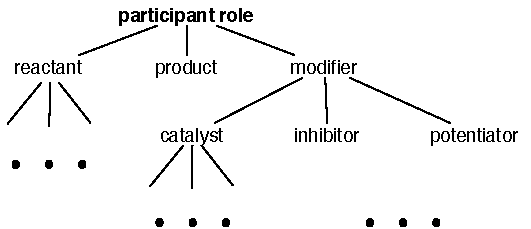
\includegraphics[scale = 0.9]{figs/sbo-participant-role}
  \end{blockMarkChanged}
  \caption{Partial expansion of some of the terms in the
    \emph{participant role} CV of SBO.}
  \label{fig:expanded-species}
\end{figure}

Figure~\ref{fig:expanded-species} shows the anticipated structure
for the \emph{participant role} CV which reflects the hierarchical
conceptual groupings of the concepts. For example, in reaction
rate expressions, there are a variety of possible modifiers.  Some
classes of modifiers can be further subdivided and grouped.  All
of this is easy to capture in the CV.  As more agreement is reached
in the modeling community about how to define and name modifiers
for different cases, the CV can grow to accommodate it.

\begin{figure}[tbh]
  \vspace*{2ex}
  \centering
  \begin{blockMarkChanged}
    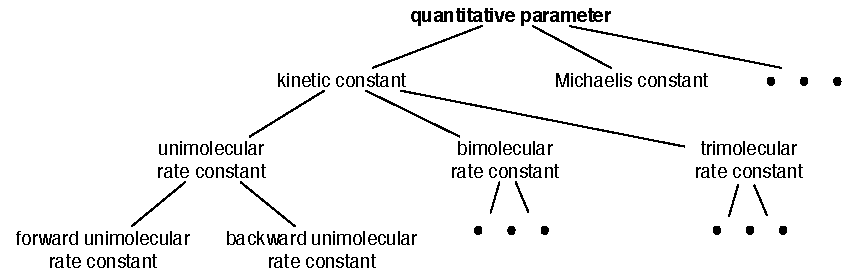
\includegraphics[scale = 0.9]{figs/sbo-quantitative-parameter}
  \end{blockMarkChanged}
  \caption{Partial expansion of some of the terms in the \emph{quantitative
      parameter} CV.}
  \label{fig:expanded-parameter}
\end{figure}

Similar to the above, the controlled vocabulary for quantitative
parameters also has a hierarchical structure, as illustrated in
Figure~\ref{fig:expanded-parameter}.  Note the separation of
\emph{kinetic constant} into separate terms for unimolecular,
bimolecular, etc. reactions, as well as for for forward and
reverse reactions.  The need to have separate terms for forward
and reverse rate constants arises in reversible mass-action
reactions.  This distinction is not always necessary for all
quantitative parameters; for example, there is no comparable
concept for the Michaelis constant.  Another distinction for some
quantitative parameters is a decomposition into different versions
based on the modeling framework being assumed.  For example,
different terms for continuous and discrete formulations of
kinetic constants represent specializations of the constants for
particular simulation frameworks.  Not all quantitative parameters
will need to be distinguished along this dimension.

\begin{wrapfigure}[6]{r}{2.85in}
%\begin{figure}[h]
  \centering
  \vspace*{-2ex}
  \begin{blockMarkChanged}
    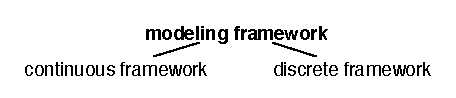
\includegraphics[scale = 0.9]{figs/sbo-framework}
  \end{blockMarkChanged}
  \vspace*{-2ex}
  \caption{Partial expansion of some of the terms in the
    \emph{modeling framework} CV.}
  \label{fig:expanded-framework}
\end{wrapfigure}
%\end{figure}
The \emph{modeling framework} controlled vocabulary is needed to
support labeling models and reactions with the framework for which
they are designed.  Figure~\ref{fig:expanded-framework}
illustrates the structure of this CV, which is at this point
extremely simple, but we expect that more terms will evolve in the
future.

Finally, there is the \emph{mathematical expression} framework.
This controlled vocabulary encompasses the various mathematical
expressions that constitute a model.
Figure~\ref{fig:sbo-math-expression} illustrates a portion of the
hierarchy.  Rate law formulas are part of the mathematical
expression hierarchy, and subdivided by successively more refined
distinctions until the leaf terms represent precise statements of
common reaction types.  Other types of mathematical expressions
are likely to be included in order to be able to characterize
other mathematical components of a model, namely initial
assignments, assignment rules, rate rules, algebraic rules,
constraints, and event triggers and assignments.

\begin{figure}[tbh]
  \centering
  \begin{blockMarkChanged}
    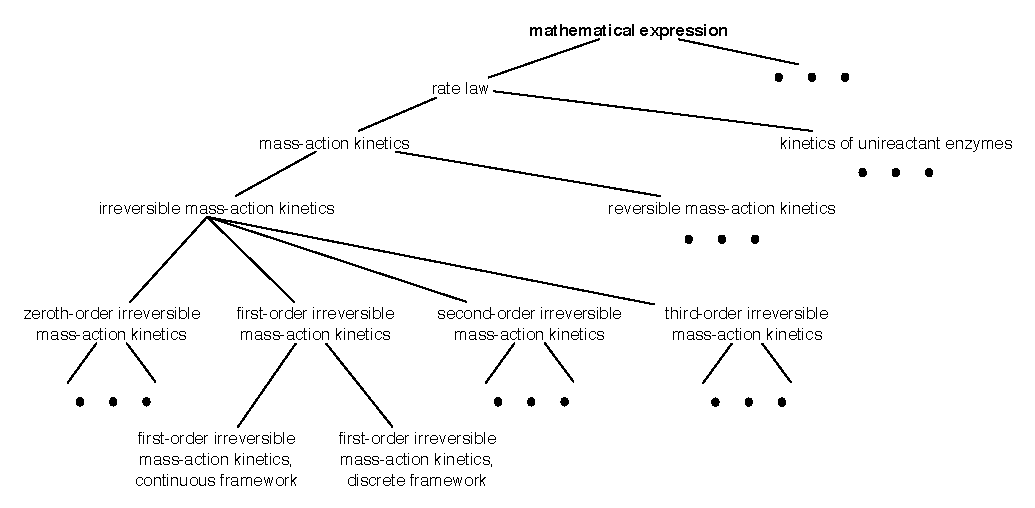
\includegraphics[scale = 0.97]{figs/sbo-math-expression}
  \end{blockMarkChanged}
  \caption{Partial expansion of some of the terms in the \emph{mathematical
      expression} CV.}
  \label{fig:sbo-math-expression}
\end{figure}

The leaf terms of the rate law portion of the SBO mathematical
expression framework contain the mathematical formulas for the
rate laws encoded using \mathmltwo.  There are many potential uses
for this.  One is to allow a software application to obtain the
formula and insert it into a model.  In effect, the formulas given
in the CV act as templates for what to put into an SBML
\KineticLaw definition.  The MathML definition also acts as a
precise statement about the rate law in question.

To make this discussion concrete, here is an example definition of
an entry in the SBO rate law hierarchy at the time of this
writing.  This term represents second-order, irreversible,
mass-action kinetics with one reactant, formulated for use in a
continuous modeling framework:
\begin{quote}
\begin{description}

\item \emph{ID}: \token{SBO:0000052}

\item \emph{Name}: second order irreversible mass action kinetics,
  one reactant, continuous scheme

\item \emph{Definition}: Reaction scheme where the products are
  created from the reactants and the change of a product quantity
  is proportional to the product of reactant activities. The
  reaction scheme does not include any reverse process that
  creates the reactants from the products, and the change of a
  product quantity is proportional to the square of one reactant
  quantity. It is to be used in a reaction modeled using a
  continuous framework.

\item \emph{Parent(s)}: \token{SBO:0000052}, first-order
  irreversible mass-action kinetics (is a)

\item \emph{MathML}:
\begin{example}
<math xmlns="http://www.w3.org/1998/Math/MathML">
   <lambda>
     <bvar><ci definitionURL="http://biomodels.net/SBO/#SBO:0000036">k</ci></bvar>
     <bvar><ci definitionURL="http://biomodels.net/SBO/#SBO:0000010">R</ci></bvar>
     <apply>
         <times/>
         <ci>k</ci>
         <ci>R</ci>
         <ci>R</ci>
     </apply>
   </lambda>
</math>
\end{example}

\end{description}
\end{quote}

In the MathML definition of the term shown above, the bound
variables in the \token{lambda} expression are tagged with
references to terms in the SBO quantitative parameter (for
\token{k}) and SBO participant role (for \token{R}) vocabularies.
This makes it possible for software applications to interpret the
intended meanings of the parameters in the expression.


%\subsubsection{Interacting with the Systems Biology Ontology}

%We fully anticipate that web service interfaces and software
%libraries will be made available to provide application
%programming interfaces (APIs) to the Systems Biology Ontology,
%allowing software applications to access definitions of SBO terms
%and relationships between them.  The actual SBO ontology is stored
%in a database, but it may be helpful to discuss the content of the
%entries in order to get a sense for the kinds of data fields that
%are likely to be available for each entry in SBO.  The following
%are the minimum anticipated data fields:
%\begin{itemize}\setlength{\parskip}{-0.2ex}

%\item \emph{Identifier}: Each term has a unique identifier of type
%  \primtype{SBOType} (Section~\ref{sec:sboterm-type}).

%\item \emph{Name}: Each term is given a name; \eg ``unimolecular
%  rate constant''.

%\item \emph{Definition}: Each term includes a written description
%  of its intended meaning.  For example, for ``unimolecular rate
%  constant'', this might be ``Numerical parameter that quantifies
%  the velocity of a chemical reaction involving only one
%  reactant.''

%\item \emph{MathML}: For terms that represent final mathematical
%  expressions (\ie the leaf terms of \sbomathformula), the formula
%  is represented using generic \mathmltwo.

%\item \emph{Parents}: The term(s) from which a given term is
%  derived.  The given term has an ``is a'' relationship to its
%  parents.

%\item \emph{Comment}: Additional notable information about the
%  CV term, on an as-needed basis.

%\end{itemize}

%Note that the definitions of formulas, in particular the rate
%laws, are recorded in generic \mathmltwo format.  They
%purposefully do not contain SBML markup.  This permits other,
%non-SBML-aware software applications to use SBO for other
%purposes, and likewise, for other kinds of ontologies to interlink
%with SBO.

One of the goals of SBO is to permit a tool to traverse up and
down the hierarchy in order to find equivalent terms in different
frameworks.  The hope is that when a software tool encounters a
given rate formula in a model, the formula will be a specific form
(say, ``mass-action kinetics, second order, one reactant, for
discrete simulation''), but by virtue of the consistent
organization of the reaction rate CV into framework-specific
definitions, the tool should in principle be able to determine the
definitions for other frameworks (say, ``mass-action kinetics,
second order, one reactant for \emph{continuous} simulation'').
If the software tool is designed for continuous simulation and it
encounters an SBML model with rate laws formulated for discrete
simulation, it could in principle look up the rate laws'
identifiers in the CV and search for alternative definitions
intended for discrete simulation.  And of course, the converse is
true, for when a tool designed for discrete simulation encounters
a model with rate laws formulated for continuous simulation.


\subsubsection{Relationships between individual SBML components and SBO terms}

The availability of \token{sboTerm} fields on various SBML
components is limited to those for which an SBO label is
appropriate given the goals and principles of SBO's use in SBML
(Section~\ref{sec:sbo-principles}).
Table~\ref{tab:sboterm-availability} summarizes the relationship
between SBML components having \token{sboTerm} fields and the
vocabularies within SBO that apply to that component.

% NOTE: make sure the list in this table matches what's
% defined in \sboelements at the top of this file.

\begin{table}[bht]
  \small
  \centering
  \begin{edtable}{tabular}{lll}
    \toprule
    \textbf{SBML Component}   & \textbf{SBO Vocabulary} & \textbf{Parent SBO Identifier} \\
    \midrule
    \Model                    & modeling framework      & \sboframeworkID \\
    \Reaction                 & modeling framework      & \sboframeworkID \\
    \Parameter                & quantitative parameter  & \sboparameterID \\
    \SpeciesReference         & participant role        & \sboparticipantID \\
    \ModifierSpeciesReference & participant role        & \sboparticipantID \\
    \FunctionDefinition       & mathematical expression & \sbomathformulaID \\
    \KineticLaw               & mathematical expression & \sbomathformulaID \\
    \InitialAssignment        & mathematical expression & \sbomathformulaID \\
    \AlgebraicRule            & mathematical expression & \sbomathformulaID \\
    \AssignmentRule           & mathematical expression & \sbomathformulaID \\
    \RateRule                 & mathematical expression & \sbomathformulaID \\
    \Constraint               & mathematical expression & \sbomathformulaID \\
    \Event                    & mathematical expression & \sbomathformulaID \\
    \EventAssignment          & mathematical expression & \sbomathformulaID \\
    \bottomrule
  \end{edtable}
  \caption{SBML components and the main types of SBO terms that
  may be assigned to them.  The parent identifiers are provided
  for guidance, but actual annotations should use more specific
  child terms.  See text for explanation.}
  \label{tab:sboterm-availability}
\end{table}

The parent identifiers shown in
Table~\ref{tab:sboterm-availability} are provided for reference.
They are the highest-level terms in their respective vocabularies;
however, these are \emph{not} the terms that would be used to
annotate an element in SBML, because there are more specific terms
underneath the parents shown here.  A software tool should use the
most specific SBO term available for a given concept rather than
using the top-level identifier acting as the root of that
particular vocabulary.

%\subsubsection{Examples}
%\label{sec:sboterm-examples}

%% FIXME

%\textbf{NEED EXAMPLES}


\subsection{Relationships to the SBML \token{annotation} field}

Another means of providing this kind of information would be to
place it inside the \token{annotation} field
(Sections~\ref{sec:sbase} and~\ref{sec:annotation-standard}).
Although \token{sboTerm} is just another kind of optional
annotation in SBML, the SBO references are separated out and given
a separate field on SBML components, both to simplify their use
for software tools and because they assert a slightly stronger and
more focused connection in a more regimented fashion.  SBO term
references are intended to allow a modeler to make a statement of
the form ``this object is identical in meaning and intention to
the definition of X in the SBO vocabulary'' and do so in a way
that a \emph{software tool can interpret unambiguously}.


\subsubsection{Tradeoffs in using SBO terms}

The SBO-based approach to annotating SBML components with
controlled terms has the following strengths:
\begin{enumerate}

\item The syntax is minimally intrusive and maximally simple,
  requiring only one string-valued attribute.

\item It supports a significant fraction of what SBML users have wanted
  to do with controlled vocabularies.

\item It does not interfere with any other scheme.  The more
  general annotation-based approach described in
  Section~\ref{sec:annotation-standard} can still be used
  simultaneously in the same model.

\end{enumerate}

The scheme has the following weaknesses:
\begin{enumerate}

\item An object can only have one \token{sboTerm} field,
  therefore, it can only be related to a single term in SBO.
  (This also impacts the design of SBO: it must be structured such
  that a class of SBML elements can logically only be associated
  with one class of terms in the ontology.)

\item The only relationship that can be expressed by
  \token{sboTerm} is ``is a''.  It is not possible to represent
  different relationships (known as \emph{verbs} in
  ontology-speak).  This limits what can be expressed.

\end{enumerate}

The weaknesses are not shared by the annotation scheme described
in Section~\ref{sec:annotation-standard}.  If an application's
needs cannot be met using SBO terms, software developers should
examine the approach described in
Section~\ref{sec:annotation-standard}.


\subsubsection{When to use SBO and when to use other annotations}

The general annotation guidelines described in
Section~\ref{sec:annotation-standard} could also be used to make
references to SBO terms.  However, in the interest of making the
use of SBO in SBML maximally interoperable between software tools,
the best-practice recommendation is to place SBO references in the
\token{sboTerm} field rather than in the \token{annotation} field
of an object.

Some software applications may have their own vocabulary of terms
similar in purpose to SBO.  For maximal software interoperability,
the best-practice recommendation in SBML is nonetheless to use SBO
terms in preference to using application-specific annotation
schemes.  Software applications should therefore attempt to
translate their private terms to and from SBO terms when writing
and reading SBML, respectively.


% AF previously removed the following subsection heading, but
% I believe there needs to be a section heading here, because
% the following  don't logically belong as part of the previous
% section.  So I'm reinserting it but with a different title. [MH]

\subsection{Discussion}

Here we discuss some additional points about the SBO-based
approach.

\subsubsection{Frequency of change in the ontology}
\label{sec:sbo-frequency-of-change}

The SBO development approach follows conventional ontology
development approaches in bioinformatics.  One of the principles
being followed is that identifiers and meanings of terms in the
CVs never change and the terms are never deleted.  Where some
terms are deemed obsolete, the introduction of new terms refine or
supersede existing terms, but the existing identifiers are left in
the CV.  Thus, references never end up pointing to nonexistent
entries.  In the case where synonymous terms are merged after
agreement that multiple terms are identical, the term identifiers
are again left in the CV and they still refer to the same concept
as before.  Out-of-date terms cached or hard-coded by an
application remain usable in all cases.  (Also, with
machine-readable CV encodings and appropriate software design, it
should be possible to develop API libraries that automatically map
older terms to newer terms as the CVs evolve.)

Therefore, a model is never in danger of ending up with SBO
identifiers that cannot be dereferenced.  If an application finds
an old model with a term \token{SBO:0000065}, it can be assured
that it will be able to find this term in SBO, even if it has been
superseded by other, more preferred terms.


\subsubsection{Consistency of information}

If you have a means of linking (say) a reaction rate formula to a
term in a CV, is it possible to have an inconsistency between the
formula in the SBML model and the one defined for the CV term?
Yes, but this is not a new problem; it arises in other situations
involving SBML models already.  The guideline for these situations
is that the model must be self-contained and stand on its own.
Therefore, in cases where they differ, the definitions in the SBML
model take precedence over the definitions referenced by the CV.
In other words, the model (and its MathML) is authoritative.


\subsubsection{Implications for network access}
\label{sec:sbo-implications-for-network-access}

Must a software tool have the ability to access the network or
read the CV every time it encounters a model or otherwise works
with SBML?  No.  Since the SBO will likely stabilize and change
infrequently once a core set of terms is defined, applications can
cache the controlled vocabulary and not make network accesses to
the master SBO copy unless something forces them to (\eg detecting
a reference in a model to an SBO term that the application does
not recognize).  In addition, applications could have user
preference settings indicating how often the CV definitions should
be refreshed (similar to how modern applications provide a setting
dictating how often they should check for new versions of
themselves).  Simple applications may go further and hard code
references to terms in SBO that have reached stability and
community consensus.


\subsubsection{Implications for software tools}

What if a software tool does not pay attention to the SBO
annotations described here?  Then one is faced with exactly the
situation that exists today: the SBML model must be interpreted
as-is, without benefit of the information added by the SBO terms.
The purpose of introducing an ontology scheme and guidelines for
its use is to give tools enough information that they \emph{could}
perform added processing, if they were designed to take advantage
of that information.


\subsubsection{Is another ontology really needed?}

It may seem that developing a new, separate ontology is overkill
for the intended purpose.  However, it turns out that no existing
ontology contains the necessary details for this role in SBML.  In
particular, none of the existing ontologies provide mathematical
formulas for reaction rates.


\end{blockChanged}


\begin{blockChanged}
%=============================================================================
\section{A standard format for the \token{annotation} field}
\label{sec:finney-novere}
\label{sec:annotation-standard}
%=============================================================================

This section describes the standard non-proprietary format for
\token{annotation} elements when (a) referring to controlled
vocabulary terms and database identifiers which define and
describe biological and biochemical entities; and (b) describing
the creator of a model and its modification history. Such a
structured format should facilitate the generation of models
compliant with the MIRIAM guidelines for model
curation~\citep{le_novere:2005}.

This format should \emph{not} be used to refer to SBO terms
(Section~\ref{sec:sboTerm}), because SBO defines terms about
mathematical modeling constructs and not the biological and
biochemical entities that the mathematics represent.

This format describes the form of one of the top level elements
that could reside in a given \token{annotation} structure. As such
this format is compliant with the constraints placed on the form
of annotation elements described in
Section~\ref{sec:annotation-use}.


\subsection{Motivation}

The SBML structures described elsewhere in this document do not
have any biochemical or biological semantics.  The format
described in this section provides a scheme for linking SBML
structures to external resources so that those structures can have
such semantics.  The motivation for the introduction of this
scheme is similar to that given for the introduction of
\token{sboTerm} however this scheme is significantly more
flexible.


\subsection{XML Namespaces in the standard annotation}

This format uses a restricted form of Dublin
Core~\citep{DCMI:2003} and BioModels qualifier elements (see
\url{http://sbml.org/wiki/Biomodels_Qualifiers}) embedded in
RDF~\citep{w3c:2004}. It uses a number of external XML standards
and associated XML namespaces.
Table~\ref{tab:namespaces-for-standard-annotation} lists these
namespaces and relevant documentation on those namespaces.  The
format constrains the order of elements in these
namespaces beyond the constraints defined in the standard
definitions for those namespaces.  For each standard listed, the
format only uses a subset of the possible syntax defined by the
given standard.  Thus it is possible for an \token{annotation}
element to include XML that is compliant with those external
standards but is not compliant with the format described here.
Parsers wishing to support this format should be aware that a
valid \token{annotation} element may contain an \token{rdf:RDF}
element which is not compliant with the format described here.  A
parser should check that all aspects of the syntax defined here
before assuming that the contained data is encoded in the format.

\begin{table}[bh]
  \vspace*{3ex}
  \begin{blockChanged}
  \small
  \centering
  \begin{edtable}{tabular}{lll}
    \toprule
    Namespace Prefix & Namespace URI & Definition Document \\
    \midrule
    \token{dc} & \uri{http://purl.org/dc/elements/1.1/} & \citep{powell:2003}\\
    \token{rdf} & \uri{http://www.w3.org/1999/02/22-rdf-syntax-ns\#} & \citep{w3c:2004b} \\
    \token{dcterms} & \uri{http://purl.org/dc/terms/} & \citep{kokkelink:2002}\\
    & & \citep{DCMIUB:2005} \\
    \token{vcard} & \uri{http://www.w3.org/2001/vcard-rdf/3.0\#} & \citep{iannella:2001} \\
    \token {bqbiol} & \uri{http://biomodels.net/biology-qualifiers/} \\
    \token {bqmodel} & \uri{http://biomodels.net/model-qualifiers/} \\
    \bottomrule
  \end{edtable}
  \vspace*{-0.95ex}
  \caption{The XML standards used in the SBML standard format for annotation.
  The namespace prefix are shown to indicate only the prefix used in the main text.}
  \label{tab:namespaces-for-standard-annotation}
  \end{blockChanged}
\end{table}

%=============================================================================
\subsection{General syntax for the standard annotation}
%=============================================================================

An outline of the format syntax is shown below.

\vspace*{0.1ex}

\begin{example}
<SBML_ELEMENT +++ metaid="SBML_META_ID" +++ >
  +++
  <annotation>
    +++
    <rdf:RDF
      xmlns:rdf="http://www.w3.org/1999/02/22-rdf-syntax-ns\#"
      xmlns:dc="http://purl.org/dc/elements/1.1/"
      xmlns:dcterm="http://purl.org/dc/terms/"
      xmlns:vcard="http://www.w3.org/2001/vcard-rdf/3.0\#"
      xmlns:bqbiol="http://biomodels.net/biology-qualifiers/" \\
      xmlns:bqmodel="http://biomodels.net/model-qualifiers/" \\
    >
      <rdf:Description rdf:about="#SBML_META_ID">
        [MODEL_HISTORY]
        <RELATION_ELEMENT>
          <rdf:Bag>
            <rdf:li rdf:resource="URI" />
            ...
          </rdf:Bag>
        </RELATION_ELEMENT>
        ...
      </rdf:Description>
      +++
    </rdf:RDF>
    +++
  </annotation>
  +++
</SBML_ELEMENT>
\end{example}

The above outline shows the order of the elements. The capitalized
identifiers refer to generic strings of a particular type:
\texttt{SBML\_ELEMENT} refers to any SBML element name that can
contain an \token{annotation} element; \texttt{SBML\_META\_ID} is
a XML \primtype{ID} string; \texttt{RELATION\_ELEMENT} refers to
element names in either the namespace
\uri{http://biomodels.net/biology-qualifiers/} or
\uri{http://biomodels.net/model-qualifiers/}; and \texttt{URI} is
a URI.  \texttt{[MODEL\_HISTORY]} refers to an optional section
described in Section~\ref{sec:model-history-annotation} which can
only be present within SBML model elements. `\texttt{+++}' is a
placeholder for either no content or valid XML syntax that is not
defined by the standard annotation scheme but is consistent with
the relevant standards for the enclosing elements. `\texttt{...}'
is a placeholder for zero or more elements of the same form as the
immediately preceding element.  The precise form of whitespace and
the XML namespace prefix definitions is not constrained however
the elements and attributes must be in the namespaces shown. The
rest of this section describes the format formally in English.

In this format the annotation of an element is located in a single
\token{rdf:RDF} element contained within an SBML
\token{annotation} element. The annotation element can contain
other elements in any order as described in Section \emph{\ref{sec:annotation-use}}.
The format described in this section only defines the form of the
\token{rdf:RDF} element. The containing SBML \SBase element
must have a \token{metaid} field value. (As this attribute is of
the type \primtype{ID} its value must unique to the entire SBML
document.)

The first element of the \token{rdf:RDF} element must be an
\token{rdf:Description} element with an \token{rdf:about}
attribute. (This format doesn't define the form of subsequent
elements of the \token{rdf:RDF} element.) The value of the
\token{rdf:about} attribute must be of the form
\texttt{\#<string>} where the string component is equal to the
value of the \token{metaid} field of the containing SBML element.

The \token{rdf:Description} element can contain only an optional
model history section (see
Section~\ref{sec:model-history-annotation}) followed by a sequence
of zero or more BioModels relation elements. The optional model
history section can only be present within an SBML \Model element.
The specific type of the relation elements will vary depending on
the relationship between the SBML component and referenced
information or resource.

Although Section~\ref{sec:qualified-dc-annotation} describes the
detailed semantics of each of the relation element types, the
content of these elements follows the same form.  The BioModels
qualifiers relation elements must only contain a single
\token{rdf:Bag} element which in turn must only contain one or
more \token{rdf:li} elements.  The \token{rdf:li} elements must
only have a \token{rdf:resource} attribute containing a URI
referring to an information resource (See
Section~\ref{sec:uri-in-annotation}).

Annotations in this format can be located at different depths
within a model component as is appropriate.

%=============================================================================
\subsection{Use of URIs}
\label{sec:uri-in-annotation}
%=============================================================================

The format represents a set of relationships between the SBML
element and the resources referred to by the contained
\token{rdf:resource} attribute values.  The BioModels relation
elements simply define the type of the relationship.

For instance a \Species element representing a protein
could be annotated with a reference to the database UniProt by the
\uri{http://www.uniprot.org/\#P12999} resource identifier,
identifying exactly the protein described by the \Species
element. This identifier maps to a unique entry in UniProt which
is never deleted from the database. In the case of UniProt, this
is the ``accession'' of the entry. When the entry is merged with
another one, both ``accession'' are conserved. Similarly in a
controlled vocabulary resource, each term is associated with a
perennial identifier. The UniProt entry also possess an ``entry
name'' (the Swiss-Prot ``identifier''), a ``protein name'',
``synonyms'' etc. Only the ``accession'' is perennial and should
be used.

The value of a \texttt{rdf:resource} attribute is a URI that both
uniquely identifies the resource, and the data in the resource. In
this case the resource constraining the identifier precedes the
'\#' symbol and the term or database identifier follows the '\#'
symbol. In the above example, the resource
\uri{http://www.uniprot.org/} includes the entry P12999.

The value of the \texttt{rdf:resource} attribute is a URI, not a
URL; as such, a URI does not have to reference a physical web
object but simply identifies a controlled vocabulary term or
database object (a URI is a label that, in this case, just happens
to look like a URL). For instance, a true URL for an Internet
resource such as \uri{http://www.uniprot.org/entry/P12999} might
correspond to the URI \uri{http://www.uniprot.org/\#P12999}.

SBML does not specify how a parser is to interpret a URI. In the
case of a transformation into a physical URL, there could be
several solutions. For instance, the URI
\uri{http://www.geneontology.org/\#GO:0007268} can be translated
into:

\noindent \uri{http://www.ebi.ac.uk/ego/DisplayGoTerm?selected=GO:0007268}\\
\noindent \uri{http://www.godatabase.org/cgi-bin/amigo/go.cgi?view=details\&query=GO:0007268}\\
\noindent
\uri{http://www.informatics.jax.org/searches/GO.cgi?id=GO:0007268}

Similarly the URI \uri{http://www.ec-code.org/\#3.5.4.4}
can refer to:

\noindent \uri{http://www.ebi.ac.uk/intenz/query?cmd=SearchEC\&ec=3.5.4.4}\\
\noindent \uri{http://www.expasy.org/cgi-bin/nicezyme.pl?3.5.4.4}\\
\noindent \uri{http://www.chem.qmul.ac.uk/iubmb/enzyme/EC3/5/4/4.html}\\
\noindent \uri{http://www.genome.jp/dbget-bin/www\_bget?ec:3.5.4.4}\\
\noindent etc.

To enable interoperability, the community has agreed on an initial
set of standardized valid URI syntax rules which may be used
within the standard annotation format. This set of rules is not
part of the SBML standard but will grow independently from
specific SBML Levels and Versions. As the set changes a given URI
syntax rule will not be modified although the physical resource
associated with the rule may change. These URIs will always be
composed as \texttt{resource\#id}. The web page
\url{http://sbml.org/wiki/MIRIAM_URI_Set} lists URI syntaxes and
possible physical links to controlled vocabulary and databases.
Each entry contains a list of SBML and relation elements in which
the given URI can be appropriately embedded. To enable consistent
and thus useful links to external resources, the URI syntax rule
set must have a consistent view of the concepts represented by the
different SBML elements for the purposes of this format.  For
example as the rule set is designed to link SBML biological and
biochemical resources the rule set assumes that a \Species element
represents the concept of a biochemical entity type rather than
mathematical symbol. The URI rule list will evolve with the
evolution of databases and resources. The annotation format
described in this section does not require a simple parser of this
format to access this list.

%=============================================================================
\subsection{Relation elements}
\label{sec:qualified-dc-annotation}
%=============================================================================

To enable the format to encode different types of relationships
between SBML elements and resources, different BioModel qualifier
elements are used to enclose a set of \token{rdf:li} elements. The
relation elements imply a specific relationship between the
enclosing SBML element and the resources referenced by the
\token{rdf:li} elements.

The detailed semantics (i.e. from the perspective of automatic
parser) of the relation elements is defined by the URI list at
\url{http://sbml.org/wiki/MIRIAM_URI_Set}, and thus is outside the
scope of SBML. The URI list generally assumes that the biological
entity represented by the element is the concept linked to the
reference resource.

Several relation elements with a given tag, enclosed in the same SBML
element, each represent an alternative annotation to the SBML
element. For example two \class{bqbiol:hasPart} elements within a
\class{Species} SBML element represent two different sets of
references to the parts making up the the chemical entity
represented by the species. (The species is not made up of all the
entities represented by all the references combined).

The complete list of the qualifier elements in the Biomodels
qualifier namespaces is documented at
\url{http://sbml.org/wiki/Biomodels_Qualifiers}. The list is
divided into two namespaces one for model qualifiers
\uri{http://biomodels.net/biology-qualifiers/} (prefix used here
\token{bqbiol}) and the other for biological qualifiers
\uri{http://biomodels.net/model-qualifiers/}) (prefix used here
\token{bqmodel}.  This list will only grow i.e no element will be
removed from the list. The following is the list of elements at
the time of writing:

%\begin{figure}[htb]
%  \vspace*{2pt}
%  \centering
%\[
%%\begin{CD}
%\textrm{SBML Element}  @>{qualifier}>> \textrm{Referenced Resource} \\
%@VV{represents}V                @VV{represents}V \\
%\textrm{Biological Entity A}   @>{relationship}>>
%\textrm{Biological Entity B}
%%\end{CD}
%\]
%  \caption{How the relationship between biological
%  entities are defined using relations between resources}
%  \label{fig:lenovere-annotation}
%\end{figure}

\begin{itemize}

\item \token{bqmodel:is} The modeling object encoded by the SBML
  component is the subject of the referenced resource. For
  instance, this qualifier might be used to link the model to a
  model database.

\item \token{bqmodel:isDescribedBy} The modeling object
  encoded by the SBML component is described by
  the referenced resource. This relation might be used to link
  SBML components to the literature that describes this model or
  this kinetic law.

\item \token{bqbiol:is} The biological entity represented by the
  SBML component is the subject of the referenced resource. This
  relation might be used to link a reaction to its exact
  counterpart in KEGG or Reactome for instance.

\item \token{bqbiol:hasPart} The biological entity represented by
  the SBML component includes the subject of the referenced
  resource, either physically or logically. This relation might be
  used to link a complex to the description of its components.

\item \token{bqbiol:isPartOf} The biological entity represented by
  the SBML component is a physical or logical part of the subject
  of the referenced resource. This relation might be used to link
  a component to the description of the complex is belongs to.

\item \token{bqbiol:isVersionOf} The biological entity represented
  by the SBML component is a version or an instance of the subject
  of the referenced resource.

\item \token{bqbiol:hasVersion} The subject of the referenced
  resource is a version or an instance of the biological entity
  represented by the SBML component.

\item \token{bqbiol:isHomologTo} The biological entity represented
  by the SBML component is homolog, to the subject of the
  referenced resource, i.e. they share a common ancestor.

\item \token{bqbiol:isDescribedBy} The biological entity
  represented by the SBML component is described by the referenced
  resource. This relation should be used for instance to link a
  species or a parameter to the literature that describes the
  quantity of the species or the value of the parameter.

\end{itemize}

%In all cases using the biology qualifiers, the `object' of the
%relation is the biological or biochemical object represented by
%the enclosing SBML element. In the cases of the model qualifiers,
%the `object' of the relation is the model component encoded by the
%enclosing SBML element. The resources referenced by the
%\class{rdf:li} elements contained within the relation element are
%the `object' of the relation.

%===============================================================
\subsection{Model history}
\label{sec:model-history-annotation}
%================================================================

When enclosed in an SBML \Model element, the format described in
previous sections can include additional elements to describe the
history of the model.  This history data must occur immediately
before the first BioModels relation elements.  These additional
elements encode information on the model creator and a sequence of
dates recording changes to the model. The syntax for this section
is outlined below.

\begin{example}
<dc:creator rdf:parseType="Resource">
  <rdf:Bag>
    <rdf:li rdf:parseType="Resource">
      [[
      +++
      <vCard:N rdf:parseType="Resource">
        <vCard:Family>FAMILY_NAME</vCard:Family>
        <vCard:Given>GIVEN_NAME</vCard:Given>
      </vCard:N>
      +++
      [<vCard:EMAIL>EMAIL_ADDRESS</vCard:EMAIL>]
      +++
      [<vCard:ORG>
        <vCard:Orgname>ORGANIZATION_NAME</vCard:Orgname>
      </vCard:ORG>]
      +++
      ]]
    </rdf:li>
    ...
  </rdf:Bag>
</dc:creator>
<dcterms:created rdf:parseType="Resource">
  <dcterms:W3CDTF>DATE</dcterms:W3CDTF>
</dcterms:created>
{<dcterms:modified rdf:parseType="Resource">
  <dcterms:W3CDTF>DATE</dcterms:W3CDTF>
</dcterms:modified>}
\end{example}

The order of elements is as shown above except that elements of
the format contained between \texttt{[[} and \texttt{]]} can occur
in any order.  The capitalized identifiers refer to generic
strings of a particular type: \texttt{FAMILY\_NAME} is the family
name of a person who created the model; \texttt{GIVEN\_NAME} is
the first name of the same person who created the model;
\texttt{EMAIL\_ADDRESS} is the email address of the same person
who created the model; and \texttt{ORGANIZATION\_NAME} is the name
of the organization with which the same person who created the
model is affiliated \texttt{DATE} is a date in W3C date
format~\citep{wolf:1998}. \texttt{W3CDTF}, \texttt{N},
\texttt{ORG} and \texttt{EMAIL} are literal strings. The elements
of the format contained between \texttt{[} and \texttt{]} are
optional. `\texttt{+++}' is a placeholder for either no content or
valid XML syntax that is not defined by the standard annotation
scheme but is consistent with the relevant standards for the
enclosing elements. `\texttt{...}' is a placeholder for zero or
more elements of the same form as the immediately preceding
element. The precise form of whitespace and the XML namespace
prefix definitions is not constrained.  The remaining text in this
section describes the syntax formally in English.

The additional elements of the model history sub-format consist in
sequence of a \token{dc:creator} element, a
\token{dcterms:created} element and zero or more
\token{dcterms:modified} elements.  All these elements must have
the attribute \token{rdf:parseType} set to \texttt{Resource}.

The \token{dc:creator} element describes the person who created
the SBML encoding of the model and contains a single
\token{rdf:Bag} element.  The \token{rdf:Bag} element can contain
any number of elements however the first element must be a
\token{rdf:li} element.  The  \token{rdf:li} element can contain
any number of elements in any order.  The set of elements
contained with the \token{rdf:li} element can include the
following informative elements: \token{vCard:N},
\token{vCard:EMAIL} and \token{vCard:ORG}.  The \token{vCard:N}
contains the name of the creator and must consist of a sequence of
two elements: \token{vCard:Family} and the \token{vCard:Given}
whose content is the family (surname) and given (first) names of
the creator respectively.  The \token{vCard:N} must have the
attribute \token{rdf:parseType} set to \texttt{Resource}.  The
content of the \token{vCard:EMAIL} element must be the email
address of the creator.  The content of the \token{vCard:ORG}
element must contain a single \token{vCard:Orgname} element.  The
\token{vCard:Orgname} element must contain the name of an
organization to which the creator is affiliated.

The \token{dcterms:created} and \token{dcterms:modified} elements
must each contain a single \token{dcterms:W3CDTF} element whose
content is a date in W3C date format~\citep{wolf:1998} which is a
a profile of (restricted form of) ISO 8601.

%================================================================
\subsection{Examples}
%=================================================================

The following shows the annotation of a model with model creation
data and links to external resources:

\begin{example}
<model metaid="_180340" id="GMO" name="Goldbeter1991_MinMitOscil">
    <annotation>
        <rdf:RDF
                xmlns:rdf="http://www.w3.org/1999/02/22-rdf-syntax-ns\#"
                xmlns:dc="http://purl.org/dc/elements/1.1/"
                xmlns:dcterms="http://purl.org/dc/terms/"
                xmlns:vCard="http://www.w3.org/2001/vcard-rdf/3.0\#"
                xmlns:bqbiol="http://biomodels.net/biology-qualifiers/"
                xmlns:bqmodel="http://biomodels.net/model-qualifiers/"
        >
            <rdf:Description rdf:about="#_180340">
                <dc:creator rdf:parseType="Resource">
                    <rdf:Bag>
                        <rdf:li rdf:parseType="Resource">
                            <vCard:N rdf:parseType="Resource">
                                <vCard:Family>Shapiro</vCard:Family>
                                <vCard:Given>Bruce</vCard:Given>
                            </vCard:N>
                            <vCard:EMAIL>bshapiro@jpl.nasa.gov</vCard:EMAIL>
                            <vCard:ORG>
                                <vCard:Orgname>NASA Jet Propulsion Laboratory</vCard:Orgname>
                            </vCard:ORG>
                        </rdf:li>
                    </rdf:Bag>
                </dc:creator>
                <dcterms:created rdf:parseType="Resource">
                    <dcterms:W3CDTF>2005-02-06T23:39:40</dcterms:W3CDTF>
                </dcterms:created>
                <dcterms:modified rdf:parseType="Resource">
                    <dcterms:W3CDTF>2005-09-13T13:24:56</dcterms:W3CDTF>
                </dcterms:modified>
                <bqmodel:is>
                    <rdf:Bag>
                        <rdf:li rdf:resource="http://www.ebi.ac.uk/biomodels/#BIOMD0000000003"/>
                    </rdf:Bag>
                </bqmodel:is>
                <bqmodel:isDescribedBy>
                     <rdf:Bag>
                         <rdf:li rdf:resource="http://www.pubmed.gov/#1833774"/>
                     </rdf:Bag>
                </bqmodel:isDescribedBy>
                <bqbiol:isVersionOf>
                    <rdf:Bag>
                        <rdf:li rdf:resource="http://www.genome.jp/kegg/pathway/#hsa04110"/>
                        <rdf:li rdf:resource="http://www.reactome.org/#69278"/>
                    </rdf:Bag>
                </bqbiol:isVersionOf>
        </rdf:Description>
    </rdf:RDF>
</annotation>
\end{example}

The following example shows a \Reaction structure annotated
with a reference to its exact Reactome counterpart.

\begin{example}
<reaction id="cdc2Phospho" metaid="jb007">
  <annotation>
    <rdf:RDF
      xmlns:bqbiol="http://biomodels.net/biology-qualifiers/"
      xmlns:rdf="http://www.w3.org/1999/02/22-rdf-syntax-ns\#"
    >
      <rdf:Description rdf:about="#jb007">
        <bqbiol:is>
          <rdf:Bag>
            <rdf:li rdf:resource="http://www.reactome.org/\#170156"/>
          </rdf:Bag>
        </bqbiol:is>
      </rdf:Description>
    </rdf:RDF>
  </annotation>
  <listOfReactants>
    <speciesReference species="cdc2"/>
  </listOfReactants>
  <listOfProducts>
    <speciesReference species="cdc2-Y15P"/>
  </listOfProducts>
  <listOfModifiers>
    <modifierSpeciesReference species="wee1"/>
  </listOfModifiers>
</reaction>
\end{example}

The following example describes a species that represents a
complex between the protein calmodulin and calcium ions:

\begin{example}
<species id="Ca_calmodulin" metaid="cacam">
  <annotation>
    <rdf:RDF
      xmlns:rdf="http://www.w3.org/1999/02/22-rdf-syntax-ns\#"
      xmlns:bqbiol="http://biomodels.net/biology-qualifiers/"
    >
      <rdf:Description rdf:about="\#cacam">
        <bqbiol:hasPart>
          <rdf:Bag>
            <rdf:li rdf:resource="http://www.uniprot.org/\#P62158"/>
            <rdf:li rdf:resource="http://www.genome.jp/kegg/compound/\#C00076"/>
          </rdf:Bag>
        </bqbiol:hasPart>
      </rdf:Description>
    </rdf:RDF>
  </annotation>
</species>
\end{example}

The following example describes a species that represents either
``Calcium/calmodulin-dependent protein kinase type II alpha
chain'' or ``Calcium/calmodulin-dependent protein kinase type II
beta chain''. This is the case for instance in the somatic
cytoplasm of striatal medium-size spiny neurons, where both are
present but they cannot be functionally differentiated.

\begin{example}
<species id="calcium_calmodulin" metaid="cacam">
  <annotation>
    <rdf:RDF
      xmlns:rdf="http://www.w3.org/1999/02/22-rdf-syntax-ns\#"
      xmlns:bqbiol="http://biomodels.net/biology-qualifiers/"
    >
      <rdf:Description rdf:about="\#cacam">
        <bqbiol:hasVersion>
          <rdf:Bag>
            <rdf:li rdf:resource="http://www.uniprot.org/\#Q9UQM7"/>
            <rdf:li rdf:resource="http://www.uniprot.org/\#Q13554"/>
          </rdf:Bag>
        </bqbiol:hasVersion>
      </rdf:Description>
    </rdf:RDF>
  </annotation>
</species>
\end{example}

The above approach should not be used to describe ``any
Calcium/calmodulin-dependent protein kinase type II chain'',
because such an annotation requires referencing the products of
other genes such as gamma or delta. All the known proteins could
be enumerated, but such an approach would almost surely lead to
inaccuracies because biological knowledge continues to evolve.
Instead, the annotation should refer to generic information such
as Ensembl family ENSF00000000194 ``CALCIUM/CALMODULIN DEPENDENT
KINASE TYPE II CHAIN'' or PIR superfamily PIRSF000594
``Calcium/calmodulin-dependent protein kinase type~II''.

%While with \texttt{HasVersion}, the described component could
%represent several alternative, with \texttt{isVersionOf} the
%described component is one of the alternative understated by the
%referenced resource.

The following two examples show how to use the qualifier
\texttt{is Version Of}. The first example is the relationship
between a reaction and an EC code. An EC code describes an
enzymatic activity and an enzymatic reaction involving a
particular enzyme can be seen as an instance of this activity. For
instance the following reaction represents the phosphorylation of
a glutamate receptor by a complex calcium/calmodulin kinase II.

\begin{example}
<reaction id="NMDAR_phosphorylation" metaid="thx1138">
  <annotation>
    <rdf:RDF
      xmlns:bqbiol="http://biomodels.net/biology-qualifiers/"
      xmlns:rdf="http://www.w3.org/1999/02/22-rdf-syntax-ns\#"
    >
      <rdf:Description rdf:about="#thx1138">
        <bqbiol:isVersionOf>
          <rdf:Bag>
            <rdf:li rdf:resource="http://www.ec-code.org/\#2.7.1.17"/>
          </rdf:Bag>
        </bqbiol:isVersionOf>
      </rdf:Description>
    </rdf:RDF>
  </annotation>
  <listOfReactants>
    <speciesReference species="NMDAR"/>
  </listOfReactants>
  <listOfProducts>
    <speciesReference species="P-NMDAR"/>
  </listOfProducts>
  <listOfModifiers>
    <modifierSpeciesReference species="CaMKII"/>
  </listOfModifiers>
  <kineticLaw>
    <math xmlns="http://www.w3.org/1998/Math/MathML">
      <apply>
        <times/>
        <ci>CaMKII</ci>
        <ci>kcat</ci>
        <apply>
          <divide/>
          <ci>NMDAR</ci>
          <apply>
            </times>
            <ci>NMDAR</ci>
            <ci>Km</ci>
          </apply>
        </apply>
      </apply>
    </math>
    <listOfParameters>
      <parameter id="kcat" value="1"/>
      <parameter id="Km" value="5e-10"/>
    </listOfParameters>
  </kineticLaw>
</reaction>
\end{example}

The second example of the use of \class{isVersionOf} is the
complex between Calcium/calmodulin-dependent protein kinase type
II alpha chain and Calcium/calmodulin, that is only one of the
``calcium- and calmodulin-dependent protein kinase complexes''
described by the Gene Ontology term GO:0005954.

\begin{example}
<species id="CaCaMKII" metaid="C8H10N4O2">
  <annotation>
    <rdf:RDF
      xmlns:rdf="http://www.w3.org/1999/02/22-rdf-syntax-ns\#"
      xmlns:bqbiol="http://biomodels.net/biology-qualifiers/"
    >
      <rdf:Description rdf:about="\#C8H10N4O2">
        <bqbiol:isVersionOf>
          <rdf:Bag>
            <rdf:li rdf:resource="http://www.geneontology.org/\#GO:0005954"/>
          </rdf:Bag>
        </bqbiol:isVersionOf>
      </rdf:Description>
    </rdf:RDF>
  </annotation>
</species>
\end{example}

The previous case is different form the following one, although they
could seem similar at first sight. The
``Calcium/calmodulin-dependent protein kinase type II alpha
chain'' is a part of the above mentioned ``calcium- and
calmodulin-dependent protein kinase complex''.

\begin{example}
<species id="CaMKIIalpha" metaid="C10H14N2">
  <annotation>
    <rdf:RDF
      xmlns:rdf="http://www.w3.org/1999/02/22-rdf-syntax-ns\#"
      xmlns:bqbiol="http://biomodels.net/biology-qualifiers/"
    >
      <rdf:Description rdf:about="\#C10H14N2">
        <bqbiol:isPartOf>
          <rdf:Bag>
            <rdf:li rdf:resource="http://www.geneontology.org/\#GO:0005954"/>
          </rdf:Bag>
        </bqbiol:isPartOf>
      </rdf:Description>
    </rdf:RDF>
  </annotation>
</species>
\end{example}

It is possible describe a component with several alternative sets
of qualified annotations. For instance, the following species
represents a pool of  GMP, GDP and GDP. We annotate it with the
three corresponding KEGG compound identifiers but also with the
three corresponding ChEBI identifiers.  The two alternative
annotations are encoded in separate \token{hasVersion} qualifier
elements.

\begin{example}
<species id="GXP" metaid="GXP">
  <annotation>
    <rdf:RDF
      xmlns:rdf="http://www.w3.org/1999/02/22-rdf-syntax-ns\#"
      xmlns:bqbiol="http://biomodels.net/biology-qualifiers/"
    >
      <rdf:Description rdf:about="\#GXP">
        <bqbiol:hasVersion>
          <rdf:Bag>
            <rdf:li rdf:resource="http://www.ebi.ac.uk/chebi/\#CHEBI:17345"/>
            <rdf:li rdf:resource="http://www.ebi.ac.uk/chebi/\#CHEBI:17552"/>
            <rdf:li rdf:resource="http://www.ebi.ac.uk/chebi/\#CHEBI:17627"/>
          </rdf:Bag>
        </bqbiol:hasVersion>
        <bqbiol:hasVersion>
          <rdf:Bag>
            <rdf:li rdf:resource="http://www.genome.jp/kegg/compound/\#C00035"/>
            <rdf:li rdf:resource="http://www.genome.jp/kegg/compound/\#C00044"/>
            <rdf:li rdf:resource="http://www.genome.jp/kegg/compound/\#C00144"/>
          </rdf:Bag>
        </bqbiol:hasVersion>
      </rdf:Description>
    </rdf:RDF>
  </annotation>
</species>
\end{example}

The following example presents a reaction being actually the
combination of three different elementary molecular reactions. We
annotate it with the three corresponding KEGG reactions, but also
with the three corresponding enzymatic activities.  Again the two
\class{hasPart} elements represent two alternative annotations.
The process represented by the \class{Reaction} structure is
composed of three parts, and  not six parts.

\begin{example}
<reaction id="adenineProd" metaid="adeprod">
  <annotation>
    <rdf:RDF
      xmlns:bqbiol="http://biomodels.net/biology-qualifiers/"
      xmlns:rdf="http://www.w3.org/1999/02/22-rdf-syntax-ns\#"
    >
      <rdf:Description rdf:about="\#adeprod">
        <bqbiol:hasPart>
          <rdf:Bag>
            <rdf:li rdf:resource="http://www.ec-code.org/\#2.5.1.22"/>
            <rdf:li rdf:resource="http://www.ec-code.org/\#3.2.2.16"/>
            <rdf:li rdf:resource="http://www.ec-code.org/\#4.1.1.50"/>
          </rdf:Bag>
        </bqbiol:hasPart>
        <bqbiol:hasPart>
          <rdf:Bag>
            <rdf:li rdf:resource="http://www.genome.jp/kegg/reaction/\#R00178"/>
            <rdf:li rdf:resource="http://www.genome.jp/kegg/reaction/\#R01401"/>
            <rdf:li rdf:resource="http://www.genome.jp/kegg/reaction/\#R02869"/>
          </rdf:Bag>
        </bqbiol:hasPart>
      </rdf:Description>
    </rdf:RDF>
  </annotation>
</reaction>
\end{example}

It is possible to mix different URIs in a given set. The
following example presents two alternative annotations of the human
hemoglobin, the first with ChEBI heme and the second with KEGG
heme.

\begin{example}
<species id="heme" metaid="heme">
  <annotation>
    <rdf:RDF
      xmlns:rdf="http://www.w3.org/1999/02/22-rdf-syntax-ns\#"
      xmlns:bqbiol="http://biomodels.net/biology-qualifiers/"
    >
     <rdf:Description rdf:about="\#heme">
       <bqbiol:hasPart>
         <rdf:Bag>
           <rdf:li rdf:resource="http://www.uniprot.org/\#P69905"/>
           <rdf:li rdf:resource="http://www.uniprot.org/\#P68871"/>
           <rdf:li rdf:resource="http://www.ebi.ac.uk/chebi/\#CHEBI:17627">
         </rdf:Bag>
       </bqbiol:hasPart>
       <bqbiol:hasPart>
         <rdf:Bag>
          <rdf:li rdf:resource="http://www.uniprot.org/\#P69905"/>
           <rdf:li rdf:resource="http://www.uniprot.org/\#P68871"/>
           <rdf:li rdf:resource="http://www.genome.jp/kegg/compound/\#C00032"/>
         </rdf:Bag>
       </bqbiol:hasPart>
     </rdf:Description>
   </rdf:RDF>
  </annotation>
</species>
\end{example}

As formally defined above it is possible to use different
qualifiers in the same annotation element. The following
phosphorylation is annotated by its exact KEGG counterpart and by
the generic GO term ``phosphorylation''.

\begin{example}
<reaction id="phosphorylation" metaid="phosphorylation">
  <annotation>
    <rdf:RDF
      xmlns:bqbiol="http://biomodels.net/biology-qualifiers/"
      xmlns:rdf="http://www.w3.org/1999/02/22-rdf-syntax-ns\#"
    >
      <rdf:Description rdf:about="\#phosphorylation">
        <bqbiol:is>
          <rdf:Bag>
            <rdf:li rdf:resource="http://www.genome.jp/kegg/reaction/\#R03313" />
          </rdf:Bag>
        </bqbiol:is>
        <bqbiol:isVersionOf>
          <rdf:Bag>
            <rdf:li rdf:resource="http://www.geneontology.org/\#GO:0016310" />
          </rdf:Bag>
        </bqbiol:isVersionOf>
      </rdf:Description>
    </rdf:RDF>
  </annotation>
</reaction>
\end{example}

\end{blockChanged}


%=============================================================================
\section{Example models expressed in XML using SBML}
\label{sec:xml-rep}
\label{sec:examples}
%=============================================================================

In this section, we present several examples of complete models
encoded in XML using SBML Level~2.

%Our approach to translating
%the UML-based structure definitions presented in the previous
%sections is described elsewhere~\citep{hucka:2000b}.
%Appendix~\ref{apdx:schemas} gives the full listing of an XML
%Schema corresponding to SBML Level~2.


%-----------------------------------------------------------------------------
\subsection{A simple example application of SBML}
\label{sec:modeleg}
%-----------------------------------------------------------------------------

\begin{blockChanged}

Consider the following representation of an enzymatic reaction:
\begin{linenomath}
\begin{reaction}\centering\notag
  E + S \eqbm^{\cit k\sub{on}}_{\cit k\sub{off}} ES \yields^{\cit k\sub{cat}} E + P
\end{reaction}
\end{linenomath}
The following is the minimal SBML document encoding the model shown above:

\sbmlexample{enzymekinetics.xml}

In this example, the model has the identifier
\val{EnzymaticReaction}.  The model contains one compartment (with
identifier \val{cytosol}), four species (with identifiers
\val{ES}, \val{P}, \val{S}, and \val{E}), and two reactions
(\val{veq} and \val{vcat}).  The elements in the
\token{listOfReactants} and \token{listOfProducts} in each
reaction refer to the names of elements listed in the
\token{listOfSpecies}.  The correspondences between the various
elements is explicitly stated by the \token{speciesReference}
elements.

The model also features local parameter definitions in each
reaction.  In this case, the three parameters (\val{kon},
\val{koff}, \val{kcat}) all have unique identifiers and they could
also have just as easily been declared global parameters in the
model.  Local parameters frequently become more useful in larger
models, where it may become tedious to assign unique identifiers
for all the different parameters.


%-----------------------------------------------------------------------------
\subsection{Example involving units}
\label{apdx:units-eg}
%-----------------------------------------------------------------------------

The following model uses the units features of SBML Level~2. In
this model, the default value of \token{substance} is changed to
be mole units with a scale factor of $-3$, or millimoles.  This
sets the default substance units in the model.  The \token{size}
and \token{time} built-ins are left to their defaults, meaning
size is in litres and time is in seconds.  The result is that, in
this model, kinetic law formulas define rates in millimoles per
second and the species identifiers in them represent concentration
values in millimoles per litres.  All the \token{species} elements
set the initial amount of every given species to 1 millimole.  The
parameters \val{vm} and \val{km} are defined to be in
millimoles per litres per second, and milliMoles per litres,
respectively.

\sbmlexample{units.xml}

\end{blockChanged}


\begin{blockChanged}
%-----------------------------------------------------------------------------
\subsection{Example of a discrete version of a simple dimerization reaction}
\label{sec:discrete-eg}
%-----------------------------------------------------------------------------

\emph{(Model contributed by Darren J. Wilkinson, Newcastle
  University, Newcastle upon Tyne, UK.)}

This example illustrates subtle differences between models
formulated for use in a continuous simulation framework (\eg using
differential equations) and those intended for a discrete
simulation framework.  The model shown here is suitable for use
with a discrete stochastic simulation algorithm of the sort
developed by \cite{gillespie:1977}.  In such an approach, species
are described in terms of molecular counts and stimulation
proceeds by computing the probability of the time and identity of
the next reaction, then updating the species amounts
appropriately.

The model involves a simple dimerization reaction for a protein
named \val{P}:
\begin{linenomath}
\begin{equation*}
    2 P  \leftrightarrow  P_2
\end{equation*}
\end{linenomath}
The SBML representation is shown below.  There are several
important points to note.  First, the species \val{P} and \val{P2}
declare they are always in discrete amounts by using the flag
\token{hasOnlySubstanceUnits}=\val{true}.  This indicates that
when the species identifiers appear in mathematical formulas, the
units are \quantity{substance}, not the default of
\quantity{substance}/\quantity{size}.  A second point is that, as
a result, the corresponding ``kinetic law'' formulas do not need
volume corrections.  In Gillespie's approach, the constants in the
rate expressions (here, \val{c1} and \val{c2}) contain a
contribution from the kinetic constants of the reaction and the
size of the compartment in which the reactions take place.
Finally, it is worth noting the rate expression for the forward
reaction is a second-order mass-action reaction, but it is the
\emph{discrete} formulation of such a reaction
rate~\citep{gillespie:1977}.

\sbmlexample{dimerization.xml}

This example also illustrates the need to provide additional
information in a model so that software tools using different
mathematical frameworks can properly interpret it.  In this case,
a simulation tool designed for continuous ODE-based simulation
would likely misinterpret the model (in particular the reaction
rate formulas), unless it deduced that a discrete stochastic
simulation was intended.  One of the purposes of SBO annotations
(Section~\ref{sec:sboTerm}) is to enable such interpretation
without the need for deduction.

\end{blockChanged}


%-----------------------------------------------------------------------------
\subsection{Example involving assignment rules}
\label{apdx:rules-eg}
%-----------------------------------------------------------------------------

This section contains a model that simulates a system containing a
fast reaction.  This model uses rules to express the mathematics
of the fast reaction explicitly rather than using the \token{fast}
field on a reaction element.  The system modeled is
\begin{linenomath}
\begin{equation*}
  \begin{array}{@{}ccc@{}}
    X_0 & \overset{\underrightarrow{k_1 X_0}}{}           & S_1 \\[6pt]
    S_1 & \overset{\underrightarrow{k_f S_1 - k_r S_2}}{} & S_2 \\[6pt]
    S_2 & \overset{\underrightarrow{k_2 S_2}}{}           & X_1 \\[6pt]
  \end{array}
\end{equation*}
\begin{equation*}
    k_1 = 0.1, \quad k_2 = 0.15, \quad k_f = K_{eq} 10000, \quad k_r = 10000, \quad K_{eq} = 2.5.
\end{equation*}
\end{linenomath}
where $X_0$, $X_1$, $S_1$, and $S_2$ are species in concentration units,
and $k_1$, $k_2$, $k_f$, $k_r$, and $K_{eq}$ are parameters.  This
system of reactions can be approximated with the following new
system:
\begin{linenomath}
\begin{equation*}
  \begin{array}{@{}ccc@{}}
    X_0 & \overset{\underrightarrow{k_1 X_0}}{} & T \\[6pt]
    T & \overset{\underrightarrow{k_2 S_2}}{} & X_1\\[6pt]
  \end{array}
\end{equation*}
\begin{equation*}
\begin{aligned}
    S_1 &= \dfrac{T}{1 + K_{eq}} \\[6pt]
    S_2 &= K_{eq} S_1
  \end{aligned}
\end{equation*}
\end{linenomath}

where $T$ is a new species.  The following example SBML model
encodes the second system.

\begin{blockChanged}
\sbmlexample{assignmentrules.xml}
\end{blockChanged}


%-----------------------------------------------------------------------------
\subsection{Example involving algebraic rules}
\label{sec:algeraiceg}
%-----------------------------------------------------------------------------

This section contains an example model that contains an
\AlgebraicRule structure.  The model contains a different
formulation of the fast reaction described in
Section~\ref{apdx:rules-eg}.  The system described in
Section~\ref{apdx:rules-eg} can be approximated with the following
system:
\begin{linenomath}
\begin{equation*}
  \begin{array}{@{}ccc@{}}
    X_0 & \overset{\underrightarrow{k_1 X_0}}{} & T \\[6pt]
    T & \overset{\underrightarrow{k_2 S_1}}{} & X_1
  \end{array}
\end{equation*}
\begin{equation*}
    S_2 = K_{eq} S_1\\[10pt]
\end{equation*}
\end{linenomath}
with the constraint:
\begin{linenomath}
\begin{equation*}
    S_1 + S_2 - T = 0
\end{equation*}
\end{linenomath}

The following example SBML model encodes this approximate form.

\begin{blockChanged}
\sbmlexample{algebraicrules.xml}
\end{blockChanged}


%-----------------------------------------------------------------------------
\subsection{Example with combinations of
  \token{boundaryCondition} and \token{constant} values on \class{Species}
  with \class{RateRule} structures}
\label{sec:constantspecieseg}
%-----------------------------------------------------------------------------

In this section, we discuss a model that includes four species,
each with a different combination of values for their
\token{boundaryCondition} and \token{constant} fields.  The
model represents a hypothetical system containing one reaction,
\begin{linenomath}
\begin{equation*}
  \begin{array}{@{}ccc@{}}
    S_1 + S_2 & \overset{\underrightarrow{k_1 S_1 S_2 S_3}}{} & S_4 \\ \\[-4pt]
  \end{array}
\end{equation*}
\end{linenomath}
where $S_3$ is a species that catalyzes the conversion of species
$S_1$ and $S_2$ into $S_4$.  $S_1$ and $S_2$ are on the boundary
of the system (\ie $S_1$ and $S_2$ are reactants but their values
are not determined by a kinetic law).  The value of $S_1$ in the
system is determined over time by the rate rule:
\begin{linenomath}
\begin{equation*}
  \dfrac{d S_1}{d t} = k_2
\end{equation*}
\end{linenomath}
The values of constant parameters in the system are:
\begin{linenomath}
\begin{equation*}
    S_2 = 1, \quad S_3 = 2, \quad k_1 = 0.5, \quad k_2 = 0.1
  \end{equation*}
\end{linenomath}
and the initial values of species are:
\begin{linenomath}
\begin{equation*}
    S_1 = 0, \quad S_4 = 0
\end{equation*}
\end{linenomath}

The value of $S_1$ varies over time so in SBML $S_1$ has a
\token{constant} field with a default value of \val{false}.  The
values of $S_2$ and $S_3$ are fixed so in SBML they have a
\token{constant} field values of \val{true}.  $S_3$ only occurs as
a modifier so the value of its \token{boundaryCondition} field can
default to \val{false}.  $S_4$ is a product whose value is
determined by a kinetic law and therefore in the SBML
representation has \val{false} (the default) for both its
\token{boundaryCondition} and \token{constant} fields.

The following is the SBML rendition of the model shown above:

\begin{blockChanged}
\sbmlexample{boundarycondition.xml}
\end{blockChanged}


\begin{blockChanged}
%-----------------------------------------------------------------------------
\subsection{Example of translation from a multi-compartmental model to ODEs}
\label{sec:odeeg}
%-----------------------------------------------------------------------------

This section contains a model with 2 compartments and 4 reactions.
The model is derived from Lotka-Volterra, with the addition of a
reversible transport step.  When observed in a time-course
simulation, three of this model's species display damped
oscillations.

\begin{figure}[htb]
  \vspace*{5pt}
  \centering
  \begin{picture}(260,60)
    \put(0,10){\framebox(255,50)[tl]{ cytosol}}
    \put(10,19){\framebox(105,29)[tl]{ nucleus}}
    \put(24,26){$
        X + Y_{1n} \yields^{\cit k\sub{1}} 2\,Y_{1n}
        \eqbm^{\cit K\sub{T}} 2\,Y_{1c} + 2\,Y_2
        \yields^{\cit k\sub{2}} 4\,Y_2 \yields^{\cit k\sub{3}} \emptyset
        $}
  \end{picture}
  \vspace*{-8pt}
  \caption{A example multi-compartmental model.}
  \label{fig:multicomp}
\end{figure}

Figure~\ref{fig:multicomp} illustrates the arrangement of
compartments and reactions in the model
\token{LotkaVolterra\_tranport}.  The text of the SBML
representation of the model is shown below, and it is followed by
its complete translation into ordinary differential equations.  In
this SBML model, the reaction equations are in substance per time
units.  The reactions have also been simplified to reduce common
stoichiometric factors.  The species variables are in
concentration units; their initial quantities are declared using
the attribute \token{initialAmount} on the \token{species}
definitions, but since the attribute \token{hasOnlySubstanceUnits}
is \emph{not} set to true, the identifiers of the species
represent their concentrations when those identifiers appear in
mathematical expressions elsewhere in the model.  Note that the
species whose identifier is \val{X} is a boundary condition, as
indicated by the attribute \token{boundaryCondition}=\val{true} in
its definition.  The attribute \token{speciesType}=\val{Y} in the
definitions of \val{Y1n} and \val{Y1c} indicates that these
species are pools of the same participant, but located in
different compartments.

\sbmlexample{multicomp.xml}

The ODE translation of this model is as follows.  First, we give
the values of the constant parameters:
\begin{linenomath}
\begin{equation*}
  k_1 = 2500, \quad k_2 = 2500, \quad K_3 = 25000, \quad K_T = 2500
\end{equation*}
\end{linenomath}
Next, here are the initial conditions of the variables.  The
species variables $X$, $Y_{1n}$, $Y_{1c}$, and $Y_2$ in the following
equations are all in terms of concentrations, and we use $V_n$ to
represent for the size of compartment \val{nucleus} and $V_c$ to
represent for the size of compartment \val{cytoplasm}:
\begin{linenomath}
\begin{equation*}
  V_n = 1, \quad V_c = 5, \quad X = 1, \quad Y_{1n} = 1, \quad Y_{1c} = 0, \quad Y_2 = 1
\end{equation*}
\end{linenomath}
And finally, here are the differential equations:
\begin{linenomath}
\begin{align*}
  \dfrac{d X}{d t}    &= 0 \\[6pt]
  V_n \dfrac{d Y_{1n}}{d t} &= k_1 \cdot X \cdot Y_{1n} \cdot V_n - K_T \cdot (Y_{1n} - Y_{1c}) \cdot V_c
    && \text{reactions production and transport} \\[6pt]
  V_c \dfrac{d Y_{1c}}{d t} &= K_T \cdot (Y_{1n} - Y_{1c}) \cdot V_c - k_2 \cdot Y_{1c} \cdot Y_2 \cdot V_c
    && \text{reactions transport and transformation} \\[6pt]
  V_c \dfrac{d Y_2}{d t}   &= k_2 \cdot Y_{1c} \cdot Y_2 \cdot V_c - k_3 \cdot Y_2 \cdot V_c
    && \text{reactions transformation and degradation}
\end{align*}
\end{linenomath}

As formulated here, this example assumes constant volumes.  If the
sizes of the compartments \val{cytoplasm} or \val{nucleus} could
change during simulation, then it would be preferable to use a
different approach to constructing the differential equations.  In
this alternative approach, the ODEs would compute substance change
rather than concentration change, and the concentration values
would be computed using separate equations.  This approach is used
in Section~\ref{sec:about-kinetic-laws}.

\end{blockChanged}


%-----------------------------------------------------------------------------
\subsection{Example involving function definitions}
\label{sec:functioneg}
%-----------------------------------------------------------------------------

This section contains a model that uses the function definition
feature of SBML.  Consider the following hypothetical system:
\begin{linenomath}
\begin{equation*}
  \begin{array}{@{}ccc@{}}
    S_1 & \overset{\underrightarrow{f(S_1)}}{} & S_2 \\ \\[-4pt]
  \end{array}
\end{equation*}
\end{linenomath}
where
\begin{linenomath}
\begin{equation*}
    f(x) = 2 \times x
\end{equation*}
\end{linenomath}

The following is the XML document that encodes the model shown
above:

\sbmlexample{functiondef.xml}


%-----------------------------------------------------------------------------
\subsection{Example involving \emph{delay} functions}
\label{sec:delayeg}
%-----------------------------------------------------------------------------

The following is a simple model illustrating the use of $delay$ to
represent a gene that suppresses its own expression.  The model
can be expressed in a single rule:
\begin{linenomath}
\begin{equation*}
  \frac{d P}{d t} = \dfrac{ \dfrac{1}{1 + m (P_{delayed})^q} - P }{ \tau }
\end{equation*}
\end{linenomath}
where
\begin{linenomath}
\begin{equation*}
\begin{array}{rl}
P_{delayed} & \mbox{is } delay(P, \Delta_t) \mbox{ or P at } t - \Delta_t\\
P & \mbox{is protein concentration}\\
\tau & \mbox{is the response time}\\
m & \mbox{is a multiplier or equilibrium constant}\\
q & \mbox{is the Hill coefficient}\\
\end{array}
\end{equation*}
\end{linenomath}
and the species quantities are in concentration units.
The text of an SBML encoding of this model is given below:

\begin{blockChanged}
\sbmlexample{delay.xml}
\end{blockChanged}


%-----------------------------------------------------------------------------
\subsection{Example involving events}
\label{sec:eventeg}
%-----------------------------------------------------------------------------

This section presents a simple model system that demonstrates the
use of events in SBML.  Consider a system with two genes, $k_1$
and $k_2$.  $k_1$ is initially on and $k_2$ is initially off.
When turned on, the two genes lead to the production of two
products, $P_1$ and $P_2$, respectively, at a fixed rate.  When
$P_1$ reaches a given concentration, $k_2$ switches off.  This
system can be represented mathematically as follows:
\begin{linenomath}
\begin{eqnarray*}
  \dfrac{d P_1}{d t} & = & k_1 - P_1\\[3pt]
  \dfrac{d P_2}{d t} & = & k_2 - P_2\\
  k_2 & = &
    \begin{cases}
      0 & \text{when $P_1 \leq \tau$},\\
      1 & \text{when $P_1 > \tau$}.
    \end{cases}
\end{eqnarray*}
\end{linenomath}

The initial values are:
\begin{linenomath}
\begin{equation*}
  k_1 = 1, \quad k_2 = 0, \quad \tau = 0.25, \quad P_1 = 0, \quad P_2 = 0
\end{equation*}
\end{linenomath}

The SBML Level 2 representation of this as follows:

\sbmlexample{events.xml}


%-----------------------------------------------------------------------------
\subsection{Example involving two-dimensional compartments}
\label{sec:two-dimensional-eg}
%-----------------------------------------------------------------------------

The following example is a model that uses a two-dimensional
compartment.  It is a fragment of a larger model of calcium
regulation across the plasma membrane of a cell.  The model
includes a calcium influx channel, \val{Ca\_channel}, and a
calcium-extruding PMCA pump, \val{Ca\_Pump}.  It also includes two
cytosolic proteins that buffer calcium via the
\val{CalciumCalbindin\_gt\_BoundCytosol} and
\val{CalciumBuffer\_gt\_BoundCytosol} reactions.  Finally, the
rate expressions in this model do not include explicit factors of
the compartment volumes; instead, the various rate constants are
assume to include any necessary corrections for volume.

\sbmlexample{twodimensional.xml}


%%-----------------------------------------------------------------------------
%\subsection{Example Using \SpeciesType Structures}
%\label{sec:speciesType-eg}
%%-----------------------------------------------------------------------------

%The following example is a model that uses \SpeciesType structures to indicate
%that 2 pools of biochemical entities (\emph{species}) located in different compartments
%contain the same type of entity (\emph{speciesType}).

%\begin{small}
%\tightspacing
%\begin{verbatim}
%<?xml version="1.0" encoding="UTF-8"?>
%<sbml xmlns="http://www.sbml.org/sbml/level2/version2" level="2" version="2">
%<model id="malate_aspartate_shuttle2">
%    <listOfCompartments>
%        <compartment id="Cytosol"/>
%        <compartment id="Mitochondrial_Matrix"/>
%    </listOfCompartments>
%    <listOfSpeciesTypes>
%        <speciesType id="Aspartate"/>
%    </listOfSpeciesTypes>
%    <listOfSpecies>
%        <species
%            id="Aspartate_in_Cytosol"
%            speciesType="Aspartate"
%            compartment="Cytosol"/>
%        <species
%            id="Aspartate_in_Mitochondrial_Matrix"
%            speciesType="Aspartate"
%            compartment="Mitochondrial_Matrix"/>
%    </listOfSpecies>
%</model>
%</sbml>
%\end{verbatim}
%\end{small}


%=============================================================================
\section{Discussion}
\label{sec:discussion}
%=============================================================================

The volume of data now emerging from molecular biotechnology
leave little doubt that extensive computer-based modeling, simulation and
analysis will be critical to understanding and interpreting the
data~\citep{abbott:1999,gilman:2000,popel:1998,smaglik:2000}.  This
has lead to an explosion in the development of computer tools by many
research groups across the world.  The explosive rate of progress is
exciting, but the rapid growth of the field is accompanied by problems and
pressing needs.

One problem is that simulation models and results often cannot be directly
compared, shared or re-used, because the tools developed by different
groups often are not compatible with each other.  As the field of systems
biology matures, researchers increasingly need to communicate their results
as computational models rather than box-and-arrow diagrams.  They also need
to reuse published and curated models as library components in order to
succeed with large-scale efforts~\citep[e.g., the Alliance for Cellular
Signaling;][]{gilman:2000,smaglik:2000}.  These needs require that models
implemented in one software package be portable to other software packages,
to maximize public understanding and to allow building up libraries of
curated computational models.

We offer SBML to the systems biology community as a suggested format for
exchanging models between simulation/analysis tools.  SBML is an open model
representation language oriented specifically towards representing systems
of biochemical reactions.

Our vision for SBML is to create an open standard that will enable
different software tools to exchange computational models.  SBML is not
static; we continue to develop and experiment with it, and we interact with
other groups who seek to develop similar markup languages.  We plan on
continuing to evolve SBML with the help of the systems biology community to
make SBML increasingly more powerful, flexible and useful.


%=============================================================================
\subsection{Future enhancements: SBML Level 3 and beyond}
\label{sec:level-3}
%=============================================================================

Many people have expressed a desire to see additional capabilities
added to SBML.  The following summarizes additional features that
are under consideration to be included in SBML Level~3:
\begin{itemize}
  
\item \emph{Arrays}.  This will enable the creation of arrays of
  components (species, reactions, compartments and submodels).
  
\item \emph{Connections}.  This will be a mechanism for describing
  the connections between items in an array.
  
\item \emph{Geometry}.  This will enable the encoding of the
  spatial characteristics of models including the geometry of
  compartments, the diffusion properties of species and the
  specification of different species concentrations across
  different regions of a cell.
  
\item \emph{Model Composition}.  This will enable a large model to
  be built up out of instances of other models.  It will also
  allow the reuse of model components and the creation of several
  instances of the same model.
  
\item \emph{Multi-state and Complex Species}.  This will allow the
  straight-forward construction of models involving species with a
  large number of states or species composed of subcomponents.
  The representation scheme would be designed to contain the
  combinatorial explosion of objects that often results from these
  types of models.

%\item \emph{Controlled Vocabularies}.  This will enable models and model components
%to be labeled with instances of controlled vocabularies.  A model vocabulary
%will describe the SBML features used by a given model.
  
\item \emph{Diagrams}.  This feature will allow components to be
  annotated with data to enable the display of the model in a
  diagram.
  
\item \emph{Dynamic Structure}.  This will enable model structure
  to vary during simulation.  One aspect of this allowing rules
  and reactions to have their effect conditional on the state of
  the model system.  For example in SBML Level 2 it is possible to
  create a rule with the effect:
\begin{linenomath}
\begin{equation*}
\frac{d s}{d t} =
\left\{
\begin{array}{ll}
     0 & \mbox{if $s>0$}\\
     y & \mbox{otherwise}
\end{array}
\right.
\end{equation*}
\end{linenomath}
Dynamic restructuring would enable the expression of the following example:
\begin{linenomath}
\begin{equation*}
\begin{array}{ll}
\mbox{if $s>0$} & \dfrac{d s}{d t} = y
\end{array}
\end{equation*}
\end{linenomath}
where $s$ is not determined by the rule when $s \leq 0$.

%\item \emph{Rules for Initial Conditions}.  This will enable the encoding
%  of rules that are only executed at the start of a simulation i.e. set
%  initial conditions.  These rules will be similar to assignment rules and
%  are evaluated in the same sequence as assignment rules but only in the
%  very first instance of simulation.

\item \emph{Tie-breaking algorithm}.  This will include a
  controlled vocabulary and associated fields on models to
  indicate the simultaneous event tie-breaking algorithm required
  to correctly simulate the model.
  
\item \emph{Distributions}.  This will provide a means of
  specifying random variables and statistical distribution of
  values.

%\item \emph{Composed Units}.  This will enable a unit definition to be
%composed from one or more other unit definitions.

\end{itemize}


%%=============================================================================
%\subsection{Relationships to Other Efforts}
%\label{sec:other-efforts}
%%=============================================================================

%There are a number of ongoing efforts with similar goals as those of SBML.
%Many of them are oriented more specifically toward describing protein
%sequences, genes and related entities for database storage and search.
%These are generally not intended to be computational models, in the sense
%that they do not describe entities and behavioral rules in such a way that
%a simulation package could ``run'' the models.

%The effort perhaps closest in spirit to SBML is
%CellML\tm~\citep{hedley:2001b}.  CellML is an XML-based markup language
%designed for storing and exchanging computer-based biological models.  It
%includes facilities for representing model structure, mathematics and
%additional information for database storage and search.  Models are
%described in terms of networks of connections between discrete components,
%where a component is a functional unit that may correspond to a physical
%compartment or simply a convenient modeling abstraction.  Components
%contain variables and connections contain mappings between the variables of
%connected components.  CellML provides facilities for grouping components
%and specifying the kinds of relationships that may exist between
%components.  It also uses MathML~\citep{w3c:2000b} for expressing
%mathematical relationships between components and provides the ability to
%use ECMAScript (formerly known as JavaScript) to define functions.

%The constructs in CellML tend to be at a more abstract and general level
%than those in SBML Level~2, and describe the structure and underlying
%mathematics of cellular models in a very general way.  By contrast, SBML is
%closer to the internal object model used in model analysis software.
%Because SBML Level~2 is being developed in the context of interacting with
%a number of existing simulation packages, it is a more concrete language
%than CellML and may be better suited to its purpose of enabling
%interoperability with existing simulation tools.

%The development of SBML Level 2 has benefited from discussions with the
%developers of CellML.  The developers of SBML and CellML are actively
%engaged in ensuring that the two representations can be translated between
%each other.


%%=============================================================================
%\subsection{Tracking the XML Schema Standard}
%\label{sec:tracking-xml}
%%=============================================================================

%One of the problems in attempting to define an XML Schema for SBML is that,
%at the time of this writing, the XML Schema
%specification~\citep{biron:2000,thompson:2000} has not actually been
%finalized.  This has been another motivation for defining SBML in terms of
%abstract data structures in a UML-based notation rather than directly as an
%XML Schema.

%The moving-target status of the XML Schema standard definition requires
%that we plan to update the Schema corresponding to SBML.  The following
%is our planned approach for handling changes in the Schema standard:
%\begin{enumerate}

%\item The definition of SBML Level~2 in this document is
%independent of XML
%  Schema.  Therefore, the definition of SBML Level~2 expressed here can
%  remain the same regardless of what happens to the exact form of XML
%  Schema.  Among other benefits, this allows developers to leave their
%  programs' internal data structures unchanged in the face of possible
%  revisions in the Schema standard.

%%\item In Appendix~\ref{apdx:schemas}, we provide an XML Schema
%%  corresponding to SBML Level~2 that has been created using the current
%%  definition of XML Schema from the W3C
%%  Organization~\citep{biron:2000,thompson:2000}.
%%
%\item Whenever the definition of XML Schema is updated by the W3C in the
%  future, we will issue a revised version of the XML Schema for SBML
%  Level~2 that conform to the updated standard.  We will leave the previous
%  versions still available for reference.  The updated XML Schemas for SBML
%  Level~2 will be identical to the previous versions except where changes
%  in XML Schema force a change in the definition of the Schema for SBML
%  Level~2.

%\end{enumerate}


%=============================================================================
\setcounter{secnumdepth}{-1}
\section{Acknowledgments}
\label{sec:acknowledgements}
%=============================================================================

\begin{blockChanged}
This specification document benefited from repeated reviews and
feedback by members of the SBML Team, especially Sarah Keating,
Bruce Shapiro, Ben Bornstein, and Maria Schilstra.  We thank them
for their efforts.  We also give special thanks to Stefan Hoops,
James Schaff, Martin Ginkel, Rainer Machn\'{e}, Sven Sahle, and
Herbert Sauro for critical discussions of the mathematical theory
underlying simulations of SBML models in the final stages of
developing this specification.

The development of SBML was originally funded entirely by the
Japan Science and Technology Agency (JST) under the ERATO Kitano
Symbiotic Systems Project during the years 2000--2003.  The
principal investigators were Hiroaki Kitano and John~C.\ Doyle.
The original SBML Team was lead by Hamid Bolouri and consisted of
Hamid Bolouri, Andrew Finney, Herbert Sauro, and Michael Hucka.

We gratefully acknowledge sponsorship from many funding agencies.
Support for the continued development of SBML and associated
software, meetings and activities today comes from the following
sources: the National Institute of General Medical Sciences (USA)
via grant number GM070923; the National Human Genome Research
Institute (USA); the International Joint Research Program of NEDO
(Japan); the JST ERATO-SORST Program (Japan); the Japanese
Ministry of Agriculture; the Japanese Ministry of Education,
Culture, Sports, Science and Technology; the BBSRC e-Science
Initiative (UK); the DARPA IPTO Bio-Computation Program (USA); and
the Air Force Office of Scientific Research (USA).  Additional
support has been or continues to be provided by the California
Institute of Technology (USA), the University of Hertfordshire
(UK), the Molecular Sciences Institute (USA), and the Systems
Biology Institute (Japan).

SBML was first conceived at the JST/ERATO-sponsored \emph{First
  Workshop on Software Platforms for Systems Biology}, held in
April, 2000, at the California Institute of Technology in
Pasadena, California, USA.  The participants collectively decided
to begin developing a common XML-based declarative language for
representing models.  A draft version of the Systems Biology
Markup Language was developed by the Caltech ERATO team and
delivered to all collaborators in August, 2000.  This draft
version underwent extensive discussion over mailing lists and then
again during the \emph{Second Workshop on Software Platforms for
  Systems Biology} held in Tokyo, Japan, November 2000.  A revised
version of SBML was issued by the Caltech ERATO team in December,
2000, and after further discussions over mailing lists and in
meetings, we produced a specification for SBML
Level~1~\citep{hucka:2001}.

\sbmltwo was conceived at the \emph{5th Workshop on Software
  Platforms for Systems Biology}, held in July 2002, at the
University of Hertfordshire, UK.  The participants collectively
decided to revise the form of SBML in \sbmltwo.  The first draft
of the Level~2 Version~1 document was released in August 2002. The
final set of features in \sbmltwoone was finalized in May 2003 at
the \emph{7th Workshop on Software Platforms for Systems Biology}
in Ft.\ Lauderdale, Florida.

\sbmltwotwo was developed with contributions from so many people
constituting the worldwide \emph{SBML Forum} that we regret it has
become infeasible to list individuals by name.  We are grateful to
everyone on the
\link{http://sbml.org/forums}{sbml-discuss@caltech.edu} and
\link{http://sbml.org/forums}{libsbml-discuss@caltech.edu} mailing
lists, the creators of CellML~\citep{hedley:2001b}, the members of
the DARPA Bio-SPICE project, and the authors of the following
software SBML-aware systems:
\href{http://depts.washington.edu/ventures/UW_Technology/Emerging_Technologies/CSI.php}{BALSA},
\href{http://www.basis.ncl.ac.uk}{BASIS},
\href{http://contraintes.inria.fr/BIOCHAM/}{BIOCHAM},
\href{http://www.cis.upenn.edu/biocomp}{BioCharon},
\href{http://diana.imim.es/ByoDyn}{ByoDyn},
\href{http://www.biocyc.org}{BioCyc},
\href{http://biocomp.ece.utk.edu/tools.html}{BioGrid},
\href{http://www.biomodels.net}{BioModels},
\href{http://cellsignaling.lanl.gov/bionetgen}{BioNetGen},
\href{http://www.bioanalyticsgroup.com/}{BioPathway~Explorer},
\href{http://www.cis.upenn.edu/biocomp/new_html/biosketch.php3}{Bio
  Sketch Pad},
\href{http://www.chemengr.ucsb.edu/~ceweb/faculty/doyle/biosens/BioSens.htm}{BioSens},
\href{http://www.biospice.org}{BioSPICE~Dashboard},
\href{http://biocomp.ece.utk.edu/tools.html}{\mbox{BioSpreadsheet}},
\href{http://labs.systemsbiology.net/bolouri/software/BioTapestry/}{BioTapestry},
\href{http://www.biouml.org/}{BioUML},
\href{https://bioinformatics.musc.edu/bstlab/}{BSTLab},
\href{http://kurata21.bse.kyutech.ac.jp/cadlive/}{CADLIVE},
\href{http://celldesigner.org}{CellDesigner},
\href{http://www-aig.jpl.nasa.gov/public/mls/cellerator/}{Cellerator},
\href{http://sbml.org/software/cellml2sbml/}{CellML2SBML},\\
\href{http://www.bii.a-star.edu.sg/sbg/cellware}{\mbox{Cellware}},
\href{http://common-lisp.net/project/cl-sbml/}{CL-SBML},
\href{http://sg.ustc.edu.cn/MFA/cleml}{CLEML},
\href{http://www.copasi.org}{COPASI},
\href{http://www.msr-unitn.unitn.it/Rpty_Soft_Sim.php}{Cyto-Sim},
\href{http://www.cytoscape.org/}{Cytoscape},
\href{http://biosim.genebee.msu.su/dbsdownload_en.html}{DBsolve},
\href{http://magnet.systemsbiology.net/software/Dizzy}{Dizzy},
\href{http://ecell.sourceforge.net/}{E-CELL},
\href{http://www.jweimar.de/ecellJ}{ecellJ},
\href{http://biocomp.ece.utk.edu/}{ESS},\\
\href{http://www.mpi-magdeburg.mpg.de/projects/fluxanalyzer}{FluxAnalyzer},
\href{http://arep.med.harvard.edu/moma/FluxorPipeline.tar.gz}{Fluxor},
\href{http://www.gepasi.org/}{Gepasi},
\href{http://www.basis.ncl.ac.uk/software.html}{Gillespie2},
\href{http://www.cis.upenn.edu/biocomp/new_html/software.php3}{HSMB},
\href{http://www.cis.upenn.edu/biocomp/new_html/software.php3}{HybridSBML},
\href{http://www.insilico-biotechnology.com}{INSILICO discovery},
\href{http://numericatech.com/jacobian.htm}{JACOBIAN},
\href{http://www.sys-bio.org/}{Jarnac},
\href{http://www.sys-bio.org/}{JDesigner},
\href{http://jigcell.biol.vt.edu}{JigCell},
\href{http://nsr.bioeng.washington.edu/PLN/Members/butterw/JSIMDOC1.6/JSim_Home.stx}{JSim},
\href{http://jjj.biochem.sun.ac.za/index.html}{JWS Online},
\href{http://www.sbml.org/kegg2sbml.html}{KEGG2SBML},
\href{http://kinetikon.molgen.mpg.de/main}{Kineticon},
\href{http://www.sbml.org/software/libsbml}{libSBML},
\href{http://www.sbml.org/mathsbml.html}{MathSBML},
\href{http://mesord.sourceforge.net/}{MesoRD},\\
\href{http://www.metabologica.com}{MetaboLogica},
\href{http://mbel.kaist.ac.kr/mfn/}{MetaFluxNet},
\href{http://www.simtec.mb.uni-siegen.de/software_mmt2.0.html}{MMT2},
\href{http://bioinformatics.oxfordjournals.org/cgi/content/abstract/20/3/316?maxtoshow=&HITS=10&hits=10&RESULTFORMAT=&fulltext=kiehl&searchid=1130434154165_1865&stored_search=&FIRSTINDEX=0&journalcode=bioinfo}{Modesto},
\href{http://www.molsci.org/~lok/moleculizer/}{Moleculizer},
\href{http://monod.molsci.org}{Monod},
\href{http://narrator-tool.org}{Narrator},
\href{http://strc.herts.ac.uk/bio/maria/NetBuilder/}{NetBuilder},
\href{http://oscill8.sf.net}{Oscill8},\\
\href{https://panther.appliedbiosystems.com/pathway/}{PANTHER
  Pathway}, \href{http://jubilantbiosys.com/pd.htm}{PathArt},
\href{http://eminch.gmxhome.de/pathscout11}{PathScout},
\href{http://innetics.com/}{PathwayLab},
\href{http://bioinformatics.ai.sri.com/ptools/}{Pathway~Tools},
\href{http://biospice.lbl.gov/PathwayBuilder/}{PathwayBuilder},
\href{http://patika.org}{PATIKAweb},
\href{http://pavesy.mpimp-golm.mpg.de}{PaVESy},
\href{http://mpf.biol.vt.edu/software/homegrown/pet/}{PET},
\href{http://page.mi.fu-berlin.de/~trieglaf/PNK2e/index.html}{PNK},
\href{http://www.reactome.org/}{Reactome},
\href{http://www.integrativebioinformatics.com/processdb.html}{ProcessDB},
\href{http://tunicata.techfak.uni-bielefeld.de/proton}{PROTON},
\href{http://www.basis.ncl.ac.uk/software.html}{pysbml},
\href{http://pysces.sourceforge.net}{PySCeS},
\href{http://ariadnegenomics.com/technology/simulation.html}{runSBML},
\href{http://sabio.villa-bosch.de/SABIORK/}{SABIO-RK},\\
\href{http://www.tbi.univie.ac.at/~raim/odeSolver/}{SBML ODE
  Solver}, \href{http://sysbio.molgen.mpg.de/SBML-PET/}{SBML-PET},
\href{http://www.ebi.ac.uk/compneur-srv/SBMLeditor.html}{SBMLeditor},
\href{http://sysbio.molgen.mpg.de/sbmlmerge/}{SBMLmerge},
\href{http://epbi-radivot.cwru.edu/}{SBMLR},
\href{http://www.dim.uchile.cl/~dremenik/SBMLSim/}{SBMLSim},
\href{http://sbml.org/software/sbmltoolbox}{SBMLToolbox},
\href{http://www-timc.imag.fr/timb/SBliD/}{SBliD},
\href{http://www.sbtoolbox.org/}{SBToolbox},
\href{http://sbw.kgi.edu/}{SBW},
\href{http://www.ucl.ac.uk/oncology/MicroCore/microcore.htm}{SCIpath},
\href{http://www.sigpath.org}{SigPath},
\href{http://depts.washington.edu/ventures/UW_Technology/Emerging_Technologies/CSI.php}{SigTran},
\href{http://www.ifak-system.com/swt/simulation/index.php?level=swtSIMBA4}{SIMBA},
\href{http://www.mathworks.com/products/simbiology/}{SimBiology},
\href{http://bioinformatics.nyu.edu/Projects/Simpathica/}{Simpathica},
\href{http://projects.villa-bosch.de/bcb/software/software/Ulla/SimWiz/}{SimWiz},
\href{http://sloppycell.sourceforge.net/}{SloppyCell},\\
\href{http://smartcell.embl.de}{SmartCell},
\href{http://www.lionbioscience.com/solutions/e20472/srspathwayeditor}{SRS
  Pathway Editor},
\href{http://www.pdn.cam.ac.uk/comp-cell/StochSim.html}{StochSim},
\href{http://www.engineering.ucsb.edu/~cse/StochKit/}{StochKit},
\href{http://www.sysbio.pl/stocks/}{STOCKS},
\href{http://teranode.com/products/index.php}{TERANODE~Suite},
\href{http://www.sourceforge.net/projects/trelis}{Trelis},
\href{http://www.vcell.org}{Virtual Cell},
\href{http://webcell.kaist.ac.kr/}{WebCell},
\href{http://www.sys-bio.org/}{WinSCAMP}, and
\href{http://www.math.pitt.edu/~bard/xpp/xpp.html}{XPPAUT}.
\end{blockChanged}

%BASIS, BioSketchPad, BioSpice, CellDesigner, Cellerator, CellML,
%COPASI, DBSolve, E-Cell, ESS, Gepasi, Jarnac, JDesigner, JigCell, MCell,
%NetBuilder, Promot/DIVA, StochSim, and Virtual Cell, and members of the
%\texttt{sysbio} and \texttt{sbml-discuss} mailing lists.  We are
%particularly grateful to the following people for discussions, advice and
%comments: Nicolas Allen, Adam Arkin, Hamid Bolouri, Ben Bornstein, Dennis
%Bray, Roger Brent, Steve Burbeck, Claudine Chaouiya, Kwang Cho, Athel
%Cornish-Bowden, Manuel Corpas, Autumn Cuellar, John Doyle, Serge Dronov,
%Drew Endy, David Fell, Carl Firth, Ed Frank, Akira Funahashi, Ralph Gauges,
%Martin Ginkel, Victoria Gor, Igor Goryanin, Warren Hedley, Charles Hodgman,
%Stefan Hoops, Nick Juty, Jay Kaserger, Sarah Keating, Hiroaki Kitano, Ben
%Kovitz, Andreas Kremling, Nicolas Le~Nov\`{e}re, Fred Livingston, Les Loew,
%Daniel Lucio, Joanne Matthews, Mike McCollum, Pedro Mendes, Eric Minch,
%Eric Mjolsness, David Morley, Mineo Morohashi, Poul Nielsen, Greg Peterson,
%Mark Poolman, Carole Proctor, Wayne Rindone, Sven Sahle, Takeshi Sakurada,
%Vijay Saraswat, Herbert Sauro, James Schaff, Maria Schilstra, John Schwacke,
%Cliff Shaffer, Bruce Shapiro, Tom Shimizu, Herbert Sauro, Hugh Spence,
%J\"{o}rg Stelling, Kouichi Takahashi, Masaru Tomita, Marc Vass, John Wagner,
%Jonathan Webb, J\"{o}rg Weimar, Darren Wilkinson, Olaf Wolkenhauer and Tau-Mu Yi.


%\changed{Both versions of SBML Level 2 were} created in
%collaboration with the authors of the following systems:
%\emph{BASIS}~\citep{kirkwood:2003},
%\emph{Bio Skektch Pad}~\citep{belta:2003},
%\emph{BioSpreadsheet}~\citep{mccollum_2003},
%\emph{BioSpice}~\citep{arkin:2001},
%\emph{CellDesigner}~\citep{funahashi:2003},
%\emph{Cellerator}~\citep{shapiro:2001,shapiro:2003b},
%\emph{COPASI}~\citep{mendes:2000},
%\emph{DBsolve}~\citep{goryanin:2001,goryanin:1999},
%\emph{E-CELL}~\citep{tomita:1999,tomita:2001},
%\emph{ESS}~\citep{peterson:2003},
%\emph{Gepasi}~\citep{mendes:1997,mendes:2001},
%\emph{Jarnac}~\citep{sauro:2000,sauro:1991},
%\emph{JDesigner}~\citep{sauro:2001b},
%\emph{JigCell}~\citep{vass:2003},
%\emph{MCell}~\citep{bartol:2002},
%\emph{NetBuilder}~\citep{schilstra:2002},
%\emph{PathScout}~\citep{minch_2003},
%\emph{ProMoT/DIVA}~\citep{stelling:2001},
%\emph{StochSim}~\citep{bray:2001,morton-firth:1998}, and
%\emph{Virtual Cell}~\citep{schaff:2000,schaff:2001}.
%\changed{Both versions of SBML Level 2 were} developed with the help of these
%packages' authors, as well as help and collaboration from the
%creators of CellML~\citep{hedley:2001b} and many other individuals
%listed in the Acknowledgments
%(Section~\ref{sec:acknowledgements}).



\newpage
\setcounter{secnumdepth}{2}
\appendix

%=============================================================================
\section{XML Schema for SBML}
\label{apdx:schema}
%=============================================================================

The following is an XML Schema definition for \sbmltwotwo, using
the W3C Recommendation for XML Schema version 1.0 of 2 May
2001~\citep{biron:2000,fallside:2000,thompson:2000}.  This 
Schema does not define all aspects of SBML Level 2: an SBML
document validated by this schema is not necessarily a valid SBML
Level 2 document.  Appendix~\ref{apdx:mathml-subset-schema}
contains a a schema for the SBML MathML subset.
Appendix~\ref{apdx:validation-rules} contains a list of the
remaining checks required to validate a model that is already
consistent with these two schemas.

The following schema is self-contained and makes reference to the
official XML Schema for MathML hosted at the W3.  However, for use
in software systems, it is more efficient to store the MathML
subset Schema of Appendix~\ref{apdx:mathml-subset-schema} in a
file on a user's local disk, and change the \token{schemaLocation}
value on line 27 below to refer to this local copy of the MathML
subset Schema.  Doing so will avoid requiring a network access
every time this SBML Schema is used.

\begin{footnotesize}
\tightspacing
\begin{verbatim}

<?xml version="1.0" encoding="UTF-8"?>
<xsd:schema
    targetNamespace="http://www.sbml.org/sbml/level2/version2"
    xmlns="http://www.sbml.org/sbml/level2/version2"
    xmlns:mml="http://www.w3.org/1998/Math/MathML"
    xmlns:xlink="http://www.w3.org/1999/xlink"
    xmlns:xsi="http://www.w3.org/2001/XMLSchema-instance"
    xmlns:xsd="http://www.w3.org/2001/XMLSchema"
    elementFormDefault="qualified"
    attributeFormDefault="unqualified"
    version="SBML L2 V2">
    <xsd:import
        namespace="http://www.w3.org/1998/Math/MathML"
        schemaLocation="http://www.w3.org/Math/XMLSchema/mathml2/mathml2.xsd"/>
    <xsd:annotation>
        <xsd:documentation>
\end{verbatim}
\begin{blockMarkChanged}
\begin{verbatim}
 * Filename   : sbml.xsd
 * Description: XML Schema for SBML Level 2 Version 2.
 * Author(s)  : Michael Hucka, Andrew Finney, Daniel Lucio
 * Revision   : $ Id: sbml.xsd,v 1.17 2006/09/23 02:03:39 mhucka Exp $
 * $ Source: /cvsroot/sbml/specifications/sbml-level-2/version-2/schema/sbml.xsd,v $
 * 
 * Copyright 2003-2006 California Institute of Technology, the Japan Science
 * and Technology Corporation, and the University of Hertfordshire.
 * 
 * This software is licensed according to the terms described in the file
 * named "LICENSE.txt" included with this distribution and available
 * online at http://sbml.org/xml-schemas/LICENSE.txt
\end{verbatim}
\end{blockMarkChanged}
\begin{verbatim}
        </xsd:documentation>
    </xsd:annotation>
    <!--The definition of SId follows.-->
    <xsd:simpleType name="SId">
        <xsd:annotation>
            <xsd:documentation>The type SId is used throughout
            SBML as the type of the 'id' attributes on model elements.</xsd:documentation>
        </xsd:annotation>
        <xsd:restriction base="xsd:string">
            <xsd:pattern value="(_|[a-z]|[A-Z])(_|[a-z]|[A-Z]|[0-9])*"/>
        </xsd:restriction>
    </xsd:simpleType>
\end{verbatim}
\begin{blockMarkChanged}
\begin{verbatim}
    <xsd:simpleType name="UnitSId">
        <xsd:annotation>
            <xsd:documentation>The type UnitSId is used to refer to units.</xsd:documentation>
        </xsd:annotation>
        <xsd:restriction base="SId" />
    </xsd:simpleType>
    <xsd:simpleType name="SBOTerm">
        <xsd:annotation>
            <xsd:documentation>The data type for sboTerm attribute values.</xsd:documentation>
        </xsd:annotation>
        <xsd:restriction base="xsd:string">
            <xsd:pattern value="(SBO:)([0-9]{7})"/>
        </xsd:restriction>
    </xsd:simpleType>
\end{verbatim}
\end{blockMarkChanged}
\begin{verbatim}
    <!--The definition of SBase follows.-->
    <xsd:complexType name="SBase" abstract="true">
        <xsd:annotation>
            <xsd:documentation>The SBase type is the base type of all main components in SBML.
            It supports attaching metadata, notes and annotations to components.</xsd:documentation>
        </xsd:annotation>
        <xsd:sequence>
            <xsd:element name="notes" minOccurs="0">
                <xsd:complexType>
                    <xsd:sequence>
                        <xsd:any namespace="http://www.w3.org/1999/xhtml" 
                                 minOccurs="0" maxOccurs="unbounded"
                                 processContents="skip"/>
                    </xsd:sequence>
                </xsd:complexType>
            </xsd:element>
            <xsd:element name="annotation" minOccurs="0">
                <xsd:complexType>
                    <xsd:sequence>
                        <xsd:any processContents="skip" minOccurs="0" maxOccurs="unbounded"/>
                    </xsd:sequence>
                </xsd:complexType>
            </xsd:element>
        </xsd:sequence>
        <xsd:attribute name="metaid" type="xsd:ID" use="optional"/>
    </xsd:complexType>
    <!--The definition of FunctionDefinition follows.-->
    <xsd:complexType name="FunctionDefinition">
        <xsd:complexContent>
            <xsd:extension base="SBase">
                <xsd:sequence>
                    <xsd:element ref="mml:math"/>
                </xsd:sequence>
                <xsd:attribute name="id" type="SId" use="required"/>
                <xsd:attribute name="name" type="xsd:string" use="optional"/>
\end{verbatim}
\begin{blockMarkChanged}
\begin{verbatim}
                <xsd:attribute name="sboTerm" type="SBOTerm" use="optional"/>
\end{verbatim}
\end{blockMarkChanged}
\begin{verbatim}
            </xsd:extension>
        </xsd:complexContent>
    </xsd:complexType>
    <!--The definition of UnitKind follows.-->
    <xsd:simpleType name="UnitKind">
        <xsd:restriction base="xsd:string">
            <xsd:enumeration value="ampere"/>
            <xsd:enumeration value="becquerel"/>
            <xsd:enumeration value="candela"/>
            <xsd:enumeration value="coulomb"/>
            <xsd:enumeration value="dimensionless"/>
            <xsd:enumeration value="farad"/>
            <xsd:enumeration value="gram"/>
            <xsd:enumeration value="gray"/>
            <xsd:enumeration value="henry"/>
            <xsd:enumeration value="hertz"/>
            <xsd:enumeration value="item"/>
            <xsd:enumeration value="joule"/>
            <xsd:enumeration value="katal"/>
            <xsd:enumeration value="kelvin"/>
            <xsd:enumeration value="kilogram"/>
            <xsd:enumeration value="litre"/>
            <xsd:enumeration value="lumen"/>
            <xsd:enumeration value="lux"/>
            <xsd:enumeration value="metre"/>
            <xsd:enumeration value="mole"/>
            <xsd:enumeration value="newton"/>
            <xsd:enumeration value="ohm"/>
            <xsd:enumeration value="pascal"/>
            <xsd:enumeration value="radian"/>
            <xsd:enumeration value="second"/>
            <xsd:enumeration value="siemens"/>
            <xsd:enumeration value="sievert"/>
            <xsd:enumeration value="steradian"/>
            <xsd:enumeration value="tesla"/>
            <xsd:enumeration value="volt"/>
            <xsd:enumeration value="watt"/>
            <xsd:enumeration value="weber"/>
        </xsd:restriction>
    </xsd:simpleType>
    <!--The definition of Unit follows.-->
    <xsd:complexType name="Unit">
        <xsd:complexContent>
            <xsd:extension base="SBase">
\end{verbatim}
\begin{blockMarkChanged}
\begin{verbatim}
                <xsd:attribute name="kind" type="UnitKind" use="required"/>
                <xsd:attribute name="exponent" type="xsd:int" default="1"/>
                <xsd:attribute name="scale" type="xsd:int" default="0"/>
                <xsd:attribute name="multiplier" type="xsd:double" default="1"/>
\end{verbatim}
\end{blockMarkChanged}
\begin{verbatim}
            </xsd:extension>
        </xsd:complexContent>
    </xsd:complexType>
    <!--The definition of UnitDefinition follows.-->
    <xsd:complexType name="ListOfUnits">
        <xsd:complexContent>
            <xsd:extension base="SBase">
                <xsd:sequence>
                    <xsd:element name="unit" type="Unit" maxOccurs="unbounded"/>
                </xsd:sequence>
            </xsd:extension>
        </xsd:complexContent>
    </xsd:complexType>
    <xsd:complexType name="UnitDefinition">
        <xsd:complexContent>
            <xsd:extension base="SBase">
                <xsd:sequence>
                    <xsd:element name="listOfUnits" type="ListOfUnits"/>
                </xsd:sequence>
\end{verbatim}
\begin{blockMarkChanged}
\begin{verbatim}
                <xsd:attribute name="id" type="UnitSId" use="required"/>
\end{verbatim}
\end{blockMarkChanged}
\begin{verbatim}
                <xsd:attribute name="name" type="xsd:string" use="optional"/>
            </xsd:extension>
        </xsd:complexContent>
    </xsd:complexType>
\end{verbatim}
\begin{blockMarkChanged}
\begin{verbatim}
    <!--The definition of CompartmentType follows.-->
    <xsd:complexType name="CompartmentType">
        <xsd:complexContent>
            <xsd:extension base="SBase">
                <xsd:attribute name="id" type="SId" use="required"/>
                <xsd:attribute name="name" type="xsd:string" use="optional"/>
            </xsd:extension>
        </xsd:complexContent>
    </xsd:complexType>
    <!--The definition of SpeciesType follows.-->
    <xsd:complexType name="SpeciesType">
        <xsd:complexContent>
            <xsd:extension base="SBase">
                <xsd:attribute name="id" type="SId" use="required"/>
                <xsd:attribute name="name" type="xsd:string" use="optional"/>
            </xsd:extension>
        </xsd:complexContent>
    </xsd:complexType>
\end{verbatim}
\end{blockMarkChanged}
\begin{verbatim}
    <!--The definition of Compartment follows.-->
    <xsd:complexType name="Compartment">
        <xsd:complexContent>
            <xsd:extension base="SBase">
                <xsd:attribute name="id" type="SId" use="required"/>
                <xsd:attribute name="name" type="xsd:string" use="optional"/>
\end{verbatim}
\begin{blockMarkChanged}
\begin{verbatim}
                <xsd:attribute name="compartmentType" type="SId" use="optional"/>
\end{verbatim}
\end{blockMarkChanged}
\begin{verbatim}
                <xsd:attribute name="spatialDimensions" use="optional" default="3">
                    <xsd:simpleType>
                        <xsd:restriction base="xsd:int">
                            <xsd:minInclusive value="0"/>
                            <xsd:maxInclusive value="3"/>
                        </xsd:restriction>
                    </xsd:simpleType>
                </xsd:attribute>
                <xsd:attribute name="size" type="xsd:double" use="optional"/>
\end{verbatim}
\begin{blockMarkChanged}
\begin{verbatim}
                <xsd:attribute name="units" type="UnitSId" use="optional"/>
\end{verbatim}
\end{blockMarkChanged}
\begin{verbatim}
                <xsd:attribute name="outside" type="SId" use="optional"/>
                <xsd:attribute name="constant" type="xsd:boolean" use="optional" default="true"/>
            </xsd:extension>
        </xsd:complexContent>
    </xsd:complexType>
    <!--The definition of Species follows.-->
    <xsd:complexType name="Species">
        <xsd:complexContent>
            <xsd:extension base="SBase">
                <xsd:attribute name="id" type="SId" use="required"/>
                <xsd:attribute name="name" type="xsd:string" use="optional"/>
\end{verbatim}
\begin{blockMarkChanged}
\begin{verbatim}
                <xsd:attribute name="speciesType" type="SId"  use="optional"/>
\end{verbatim}
\end{blockMarkChanged}
\begin{verbatim}
                <xsd:attribute name="compartment" type="SId" use="required"/>
                <xsd:attribute name="initialAmount" type="xsd:double" use="optional"/>
                <xsd:attribute name="initialConcentration" type="xsd:double" use="optional"/>
\end{verbatim}
\begin{blockMarkChanged}
\begin{verbatim}
                <xsd:attribute name="substanceUnits" type="UnitSId" use="optional"/>
                <xsd:attribute name="spatialSizeUnits" type="UnitSId" use="optional"/>
\end{verbatim}
\end{blockMarkChanged}
\begin{verbatim}
                <xsd:attribute name="hasOnlySubstanceUnits" type="xsd:boolean" use="optional" default="false"/>
                <xsd:attribute name="boundaryCondition" type="xsd:boolean" use="optional" default="false"/>
                <xsd:attribute name="charge" type="xsd:int" use="optional"/>
                <xsd:attribute name="constant" type="xsd:boolean" use="optional" default="false"/>
            </xsd:extension>
        </xsd:complexContent>
    </xsd:complexType>
    <!--The definition of Parameter follows.-->
    <xsd:complexType name="Parameter">
        <xsd:complexContent>
            <xsd:extension base="SBase">
                <xsd:attribute name="id" type="SId" use="required"/>
                <xsd:attribute name="name" type="xsd:string" use="optional"/>
                <xsd:attribute name="value" type="xsd:double" use="optional"/>
\end{verbatim}
\begin{blockMarkChanged}
\begin{verbatim}
                <xsd:attribute name="units" type="UnitSId" use="optional"/>
\end{verbatim}
\end{blockMarkChanged}
\begin{verbatim}
                <xsd:attribute name="constant" type="xsd:boolean" use="optional" default="true"/>
\end{verbatim}
\begin{blockMarkChanged}
\begin{verbatim}
                <xsd:attribute name="sboTerm" type="SBOTerm" use="optional"/>
\end{verbatim}
\end{blockMarkChanged}
\begin{verbatim}
            </xsd:extension>
        </xsd:complexContent>
    </xsd:complexType>
    <xsd:complexType name="ListOfParameters">
        <xsd:complexContent>
            <xsd:extension base="SBase">
                <xsd:sequence>
                    <xsd:element name="parameter" type="Parameter" maxOccurs="unbounded"/>
                </xsd:sequence>
            </xsd:extension>
        </xsd:complexContent>
    </xsd:complexType>
\end{verbatim}
\begin{blockMarkChanged}
\begin{verbatim}
    <!--The definition of Initial Assignment follows.-->
    <xsd:complexType name="InitialAssignment">
        <xsd:complexContent>
            <xsd:extension base="SBase">
                <xsd:sequence>
                    <xsd:element ref="mml:math"/>
                </xsd:sequence>
                <xsd:attribute name="symbol" type="SId" use="required"/>
                <xsd:attribute name="sboTerm" type="SBOTerm" use="optional"/>
            </xsd:extension>
        </xsd:complexContent>
    </xsd:complexType>
\end{verbatim}
\end{blockMarkChanged}
\begin{verbatim}
    <!--The definition of Rule follows. -->
    <xsd:complexType name="Rule" abstract="true">
        <xsd:complexContent>
            <xsd:extension base="SBase">
                <xsd:sequence>
                    <xsd:element ref="mml:math"/>
                </xsd:sequence>
\end{verbatim}
\begin{blockMarkChanged}
\begin{verbatim}
                <xsd:attribute name="sboTerm" type="SBOTerm" use="optional"/>
\end{verbatim}
\end{blockMarkChanged}
\begin{verbatim}
            </xsd:extension>
        </xsd:complexContent>
    </xsd:complexType>
    <xsd:complexType name="AlgebraicRule">
        <xsd:complexContent>
            <xsd:extension base="Rule"/>
        </xsd:complexContent>
    </xsd:complexType>
    <xsd:complexType name="AssignmentRule">
        <xsd:complexContent>
            <xsd:extension base="Rule">
                <xsd:attribute name="variable" type="SId" use="required"/>
            </xsd:extension>
        </xsd:complexContent>
    </xsd:complexType>
    <xsd:complexType name="RateRule">
        <xsd:complexContent>
            <xsd:extension base="Rule">
                <xsd:attribute name="variable" type="SId" use="required"/>
            </xsd:extension>
        </xsd:complexContent>
    </xsd:complexType>
\end{verbatim}
\begin{blockMarkChanged}
\begin{verbatim}
    <!--The definition of Constraint follows.-->
    <xsd:complexType name="Constraint">
        <xsd:complexContent>
            <xsd:extension base="SBase">
                <xsd:sequence>
                    <xsd:element ref="mml:math"/>
                    <xsd:element name="message" minOccurs="0">
                        <xsd:complexType>
                            <xsd:sequence>
                                <xsd:any namespace="http://www.w3.org/1999/xhtml" 
                                         minOccurs="0" maxOccurs="unbounded"
                                         processContents="skip"/>
                            </xsd:sequence>
                        </xsd:complexType>
                    </xsd:element>
                </xsd:sequence>
                <xsd:attribute name="sboTerm" type="SBOTerm" use="optional"/>
            </xsd:extension>
        </xsd:complexContent>
    </xsd:complexType>
\end{verbatim}
\end{blockMarkChanged}
\begin{verbatim}
    <!--The definition of Reaction follows.-->
    <xsd:complexType name="KineticLaw">
        <xsd:complexContent>
            <xsd:extension base="SBase">
                <xsd:sequence>
                    <xsd:element ref="mml:math"/>
                    <xsd:element name="listOfParameters" type="ListOfParameters" minOccurs="0"/>
                </xsd:sequence>
\end{verbatim}
\begin{blockMarkChanged}
\begin{verbatim}
                <xsd:attribute name="sboTerm" type="SBOTerm" use="optional"/>
\end{verbatim}
\end{blockMarkChanged}
\begin{verbatim}
            </xsd:extension>
        </xsd:complexContent>
    </xsd:complexType>
    <xsd:complexType name="SimpleSpeciesReference" abstract="true">
        <xsd:complexContent>
            <xsd:extension base="SBase">
\end{verbatim}
\begin{blockMarkChanged}
\begin{verbatim}
                <xsd:attribute name="id" type="SId" use="optional"/>
                <xsd:attribute name="name" type="xsd:string" use="optional"/>
\end{verbatim}
\end{blockMarkChanged}
\begin{verbatim}
                <xsd:attribute name="species" type="SId" use="required"/>
\end{verbatim}
\begin{blockMarkChanged}
\begin{verbatim}
                <xsd:attribute name="sboTerm" type="SBOTerm" use="optional"/>
\end{verbatim}
\end{blockMarkChanged}
\begin{verbatim}
            </xsd:extension>
        </xsd:complexContent>
    </xsd:complexType>
    <xsd:complexType name="ModifierSpeciesReference">
        <xsd:complexContent>
            <xsd:extension base="SimpleSpeciesReference"/>
        </xsd:complexContent>
    </xsd:complexType>
    <xsd:complexType name="ListOfModifierSpeciesReferences">
        <xsd:complexContent>
            <xsd:extension base="SBase">
                <xsd:sequence>
                    <xsd:element name="modifierSpeciesReference" 
                                 type="ModifierSpeciesReference" maxOccurs="unbounded"/>
                </xsd:sequence>
            </xsd:extension>
        </xsd:complexContent>
    </xsd:complexType>
    <xsd:complexType name="StoichiometryMath">
        <xsd:complexContent>
            <xsd:extension base="SBase">
                <xsd:sequence>
                    <xsd:element ref="mml:math"/>
                </xsd:sequence>
            </xsd:extension>
        </xsd:complexContent>
    </xsd:complexType>
    <xsd:complexType name="SpeciesReference">
        <xsd:complexContent>
            <xsd:extension base="SimpleSpeciesReference">
                <xsd:sequence>
                    <xsd:element name="stoichiometryMath" type="StoichiometryMath" minOccurs="0"/>
                </xsd:sequence>
                <xsd:attribute name="stoichiometry" type="xsd:double" use="optional" default="1"/>
            </xsd:extension>
        </xsd:complexContent>
    </xsd:complexType>
    <xsd:complexType name="ListOfSpeciesReferences">
        <xsd:complexContent>
            <xsd:extension base="SBase">
                <xsd:sequence>
                    <xsd:element name="speciesReference" type="SpeciesReference" maxOccurs="unbounded"/>
                </xsd:sequence>
            </xsd:extension>
        </xsd:complexContent>
    </xsd:complexType>
    <xsd:complexType name="Reaction">
        <xsd:complexContent>
            <xsd:extension base="SBase">
                <xsd:sequence>
                    <xsd:element name="listOfReactants" type="ListOfSpeciesReferences" minOccurs="0"/>
                    <xsd:element name="listOfProducts" type="ListOfSpeciesReferences" minOccurs="0"/>
                    <xsd:element name="listOfModifiers" type="ListOfModifierSpeciesReferences" minOccurs="0"/>
                    <xsd:element name="kineticLaw" type="KineticLaw" minOccurs="0"/>
                </xsd:sequence>
                <xsd:attribute name="id" type="SId" use="required"/>
                <xsd:attribute name="name" type="xsd:string" use="optional"/>
                <xsd:attribute name="reversible" type="xsd:boolean" use="optional" default="true"/>
\end{verbatim}
\begin{blockMarkChanged}
\begin{verbatim}
                <xsd:attribute name="fast" type="xsd:boolean" use="optional" default="false"/>
                <xsd:attribute name="sboTerm" type="SBOTerm" use="optional"/>
\end{verbatim}
\end{blockMarkChanged}
\begin{verbatim}
            </xsd:extension>
        </xsd:complexContent>
    </xsd:complexType>
    <!--The definition of Event follows.-->
    <xsd:complexType name="EventAssignment">
        <xsd:complexContent>
            <xsd:extension base="SBase">
                <xsd:sequence>
                    <xsd:element ref="mml:math"/>
                </xsd:sequence>
                <xsd:attribute name="variable" type="SId" use="required"/>
\end{verbatim}
\begin{blockMarkChanged}
\begin{verbatim}
                <xsd:attribute name="sboTerm" type="SBOTerm" use="optional"/>
\end{verbatim}
\end{blockMarkChanged}
\begin{verbatim}
            </xsd:extension>
        </xsd:complexContent>
    </xsd:complexType>
    <xsd:complexType name="ListOfEventAssignments">
        <xsd:complexContent>
            <xsd:extension base="SBase">
                <xsd:sequence>
                    <xsd:element name="eventAssignment" type="EventAssignment" maxOccurs="unbounded"/>
                </xsd:sequence>
            </xsd:extension>
        </xsd:complexContent>
    </xsd:complexType>
    <xsd:complexType name="MathField">
        <xsd:complexContent>
            <xsd:extension base="SBase">
                <xsd:sequence>
                    <xsd:element ref="mml:math"/>
                </xsd:sequence>
            </xsd:extension>
        </xsd:complexContent>
    </xsd:complexType>
    <xsd:complexType name="Event">
        <xsd:complexContent>
            <xsd:extension base="SBase">
                <xsd:sequence>
                    <xsd:element name="trigger" type="MathField"/>
                    <xsd:element name="delay" type="MathField" minOccurs="0"/>
                    <xsd:element name="listOfEventAssignments" type="ListOfEventAssignments"/>
                </xsd:sequence>
                <xsd:attribute name="id" type="SId" use="optional"/>
                <xsd:attribute name="name" type="xsd:string" use="optional"/>
                <xsd:attribute name="timeUnits" type="UnitSId" use="optional"/>
\end{verbatim}
\begin{blockMarkChanged}
\begin{verbatim}
                <xsd:attribute name="sboTerm" type="SBOTerm" use="optional"/>
\end{verbatim}
\end{blockMarkChanged}
\begin{verbatim}
            </xsd:extension>
        </xsd:complexContent>
    </xsd:complexType>
    <!-- The definition of Model follows.-->
    <xsd:complexType name="Model">
        <xsd:complexContent>
            <xsd:extension base="SBase">
                <xsd:sequence>
                    <xsd:element name="listOfFunctionDefinitions" minOccurs="0">
                        <xsd:complexType>
                            <xsd:complexContent>
                                <xsd:extension base="SBase">
                                    <xsd:sequence>
                                        <xsd:element name="functionDefinition" 
                                                     type="FunctionDefinition" maxOccurs="unbounded"/>
                                    </xsd:sequence>
                                </xsd:extension>
                            </xsd:complexContent>
                        </xsd:complexType>
                    </xsd:element>
                    <xsd:element name="listOfUnitDefinitions" minOccurs="0">
                        <xsd:complexType>
                            <xsd:complexContent>
                                <xsd:extension base="SBase">
                                    <xsd:sequence>
                                        <xsd:element name="unitDefinition" 
                                                     type="UnitDefinition" maxOccurs="unbounded"/>
                                    </xsd:sequence>
                                </xsd:extension>
                            </xsd:complexContent>
                        </xsd:complexType>
                    </xsd:element>
\end{verbatim}
\begin{blockMarkChanged}
\begin{verbatim}
                    <xsd:element name="listOfCompartmentTypes" minOccurs="0">
                        <xsd:complexType>
                            <xsd:complexContent>
                                <xsd:extension base="SBase">
                                    <xsd:sequence>
                                        <xsd:element
                                            name="compartmentType"
                                            type="CompartmentType"
                                            maxOccurs="unbounded"/>
                                    </xsd:sequence>
                                </xsd:extension>
                            </xsd:complexContent>
                        </xsd:complexType>
                    </xsd:element>
                    <xsd:element name="listOfSpeciesTypes" minOccurs="0">
                        <xsd:complexType>
                            <xsd:complexContent>
                                <xsd:extension base="SBase">
                                    <xsd:sequence>
                                        <xsd:element name="speciesType" type="SpeciesType" 
                                                     maxOccurs="unbounded"/>
                                    </xsd:sequence>
                                </xsd:extension>
                            </xsd:complexContent>
                        </xsd:complexType>
                    </xsd:element>
\end{verbatim}
\end{blockMarkChanged}
\begin{verbatim}
                    <xsd:element name="listOfCompartments" minOccurs="0">
                        <xsd:complexType>
                            <xsd:complexContent>
                                <xsd:extension base="SBase">
                                    <xsd:sequence>
                                        <xsd:element name="compartment" type="Compartment" 
                                                     maxOccurs="unbounded"/>
                                    </xsd:sequence>
                                </xsd:extension>
                            </xsd:complexContent>
                        </xsd:complexType>
                    </xsd:element>
                    <xsd:element name="listOfSpecies" minOccurs="0">
                        <xsd:complexType>
                            <xsd:complexContent>
                                <xsd:extension base="SBase">
                                    <xsd:sequence>
                                        <xsd:element name="species" type="Species" 
                                                     maxOccurs="unbounded"/>
                                    </xsd:sequence>
                                </xsd:extension>
                            </xsd:complexContent>
                        </xsd:complexType>
                    </xsd:element>
                    <xsd:element name="listOfParameters" type="ListOfParameters" minOccurs="0"/>
\end{verbatim}
\begin{blockMarkChanged}
\begin{verbatim}
                    <xsd:element name="listOfInitialAssignments" minOccurs="0">
                        <xsd:complexType>
                            <xsd:complexContent>
                                <xsd:extension base="SBase">
                                    <xsd:sequence>
                                        <xsd:element name="initialAssignment" 
                                                     type="InitialAssignment" maxOccurs="unbounded"/>
                                    </xsd:sequence>
                                </xsd:extension>
                            </xsd:complexContent>
                        </xsd:complexType>
                    </xsd:element>
\end{verbatim}
\end{blockMarkChanged}
\begin{verbatim}
                    <xsd:element name="listOfRules" minOccurs="0">
                        <xsd:complexType>
                            <xsd:complexContent>
                                <xsd:extension base="SBase">
                                    <xsd:choice maxOccurs="unbounded">
                                        <xsd:element name="algebraicRule" type="AlgebraicRule" 
                                                     minOccurs="0"/>
                                        <xsd:element name="assignmentRule" type="AssignmentRule" 
                                                     minOccurs="0"/>
                                        <xsd:element name="rateRule" type="RateRule" minOccurs="0"/>
                                    </xsd:choice>
                                </xsd:extension>
                            </xsd:complexContent>
                        </xsd:complexType>
                    </xsd:element>
\end{verbatim}
\begin{blockMarkChanged}
\begin{verbatim}
                    <xsd:element name="listOfConstraints" minOccurs="0">
                        <xsd:complexType>
                            <xsd:complexContent>
                                <xsd:extension base="SBase">
                                    <xsd:sequence>
                                        <xsd:element name="constraint" type="Constraint" 
                                                     maxOccurs="unbounded"/>
                                    </xsd:sequence>
                                </xsd:extension>
                            </xsd:complexContent>
                        </xsd:complexType>
                    </xsd:element>
\end{verbatim}
\end{blockMarkChanged}
\begin{verbatim}
                    <xsd:element name="listOfReactions" minOccurs="0">
                        <xsd:complexType>
                            <xsd:complexContent>
                                <xsd:extension base="SBase">
                                    <xsd:sequence>
                                        <xsd:element name="reaction" type="Reaction" 
                                                     maxOccurs="unbounded"/>
                                    </xsd:sequence>
                                </xsd:extension>
                            </xsd:complexContent>
                        </xsd:complexType>
                    </xsd:element>
                    <xsd:element name="listOfEvents" minOccurs="0">
                        <xsd:complexType>
                            <xsd:complexContent>
                                <xsd:extension base="SBase">
                                    <xsd:sequence>
                                        <xsd:element name="event" type="Event" 
                                                     maxOccurs="unbounded"/>
                                    </xsd:sequence>
                                </xsd:extension>
                            </xsd:complexContent>
                        </xsd:complexType>
                    </xsd:element>
                </xsd:sequence>
                <xsd:attribute name="id" type="SId" use="optional"/>
                <xsd:attribute name="name" type="xsd:string" use="optional"/>
\end{verbatim}
\begin{blockMarkChanged}
\begin{verbatim}
                <xsd:attribute name="sboTerm" type="SBOTerm" use="optional"/>
\end{verbatim}
\end{blockMarkChanged}
\begin{verbatim}
            </xsd:extension>
        </xsd:complexContent>
    </xsd:complexType>
    <!-- The following is the type definition for the top-level element in an SBML document.-->
    <xsd:complexType name="Sbml">
        <xsd:complexContent>
            <xsd:extension base="SBase">
                <xsd:sequence>
                    <xsd:element name="model" type="Model"/>
                </xsd:sequence>
                <xsd:attribute name="level" type="xsd:positiveInteger" use="required" fixed="2"/>
\end{verbatim}
\begin{blockMarkChanged}
\begin{verbatim}
                <xsd:attribute name="version" type="xsd:positiveInteger" use="required" fixed="2"/>
\end{verbatim}
\end{blockMarkChanged}
\begin{verbatim}
            </xsd:extension>
        </xsd:complexContent>
    </xsd:complexType>
    <!--The following is the (only) top-level element allowed in an SBML document.-->
    <xsd:element name="sbml" type="Sbml"/>
    <!--The end.-->
</xsd:schema>
\end{verbatim}
\regularspacing
\end{footnotesize}


\begin{blockChanged}
%=============================================================================
\section{XML Schema for MathML subset}
\label{apdx:mathml-subset-schema}
%=============================================================================

The following XML schema defines the syntax of the MathML syntax
that is used in SBML Level 2 version 1 and 2.

\begin{footnotesize}
\tightspacing
\begin{verbatim}

<?xml version="1.0" encoding="UTF-8"?>
<!--
 * Filename    : sbml-mathml.xsd
 * Description : Schema for the MathML subset used by SBML L2.
 * Author(s)   : Andrew Finney, Michael Hucka
 * Organization: SBML Team <sbml-team@caltech.edu>
 * Revision    : $ Id: sbml-mathml.xsd,v 1.3 2006/07/20 23:46:31 mhucka Exp $
 * Source      : $ Source: /cvsroot/sbml/specifications/sbml-mathml/sbml-mathml.xsd,v $
 *
 * Copyright 2003-2006 California Institute of Technology, the Japan Science
 * and Technology Corporation, and the University of Hertfordshire.
 *
 * This software is licensed according to the terms described in the file
 * named "LICENSE.txt" included with this distribution and available
 * online at http://sbml.org/xml-schemas/LICENSE.txt
 *
 * Summary:
 * 
 * This is a reduced version of the XML Schema for MathML 2.0.  It 
 * corresponds to the subset of MathML 2.0 used in SBML Level 2, and
 * should be used by validating XML parsers instead of the actual
 * MathML XML Schema when validating SBML files.  To accomplish that,
 * changed the value of the attribute 'schemaLocation' in the SBML
 * XML Schema file (sbml.xsd) to refer to a copy of this Schema file
 * on your computer's local hard disk.
-->
<xs:schema xmlns="http://www.w3.org/1998/Math/MathML" 
           xmlns:xsi="http://www.w3.org/2001/XMLSchema-instance" 
           xmlns:xs="http://www.w3.org/2001/XMLSchema" 
           targetNamespace="http://www.w3.org/1998/Math/MathML" 
           elementFormDefault="qualified" 
           attributeFormDefault="unqualified">
    <xs:attributeGroup name="MathAttributes">
        <xs:attribute name="class" type="xs:NMTOKENS" use="optional"/>
        <xs:attribute name="style" type="xs:string" use="optional"/>
        <xs:attribute name="id" type="xs:ID" use="optional"/>
    </xs:attributeGroup>
    <xs:complexType name="MathBase">
        <xs:attributeGroup ref="MathAttributes"/>
    </xs:complexType>
    <xs:attributeGroup name="CnAttributes">
        <xs:attribute name="type">
            <xs:simpleType>
                <xs:restriction base="xs:NMTOKEN">
                    <xs:enumeration value="e-notation"/>
                    <xs:enumeration value="integer"/>
                    <xs:enumeration value="rational"/>
                    <xs:enumeration value="real"/>
                </xs:restriction>
            </xs:simpleType>
        </xs:attribute>
        <xs:attributeGroup ref="MathAttributes"/>
    </xs:attributeGroup>
    <xs:complexType name="SepType"/>
    <xs:complexType name="Cn" mixed="true">
        <xs:choice minOccurs="0">
            <xs:element name="sep" type="SepType"/>
        </xs:choice>
        <xs:attributeGroup ref="CnAttributes"/>
    </xs:complexType>
    <xs:complexType name="Ci">
        <xs:simpleContent>
            <xs:extension base="xs:string">
                <xs:attributeGroup ref="MathAttributes"/>
            </xs:extension>
        </xs:simpleContent>
    </xs:complexType>
    <xs:simpleType name="CsymbolURI">
        <xs:restriction base="xs:string">
            <xs:enumeration value="http://www.sbml.org/sbml/symbols/time"/>
            <xs:enumeration value="http://www.sbml.org/sbml/symbols/delay"/>
        </xs:restriction>
    </xs:simpleType>
    <xs:complexType name="Csymbol">
        <xs:simpleContent>
            <xs:extension base="xs:string">
                <xs:attribute name="encoding" use="required" fixed="text"/>
                <xs:attribute name="definitionURL" type="CsymbolURI" use="required"/>
                <xs:attributeGroup ref="MathAttributes"/>
            </xs:extension>
        </xs:simpleContent>
    </xs:complexType>
    <xs:complexType name="NodeContainer">
        <xs:complexContent>
            <xs:extension base="MathBase">
                <xs:group ref="Node"/>
            </xs:extension>
        </xs:complexContent>
    </xs:complexType>
    <xs:complexType name="Apply">
        <xs:complexContent>
            <xs:extension base="MathBase">
                <xs:sequence>
                    <xs:choice>
                        <xs:element name="ci" type="Ci"/>
                        <xs:element name="csymbol" type="Csymbol"/>
                        <xs:element name="eq" type="MathBase"/>
                        <xs:element name="neq" type="MathBase"/>
                        <xs:element name="gt" type="MathBase"/>
                        <xs:element name="lt" type="MathBase"/>
                        <xs:element name="geq" type="MathBase"/>
                        <xs:element name="leq" type="MathBase"/>
                        <xs:element name="plus" type="MathBase"/>
                        <xs:element name="minus" type="MathBase"/>
                        <xs:element name="times" type="MathBase"/>
                        <xs:element name="divide" type="MathBase"/>
                        <xs:element name="power" type="MathBase"/>
                        <xs:sequence>
                            <xs:element name="root" type="MathBase"/>
                            <xs:element name="degree" type="NodeContainer" minOccurs="0"/>
                        </xs:sequence>
                        <xs:element name="abs" type="MathBase"/>
                        <xs:element name="exp" type="MathBase"/>
                        <xs:element name="ln" type="MathBase"/>
                        <xs:sequence>
                            <xs:element name="log" type="MathBase"/>
                            <xs:element name="logbase" type="NodeContainer" minOccurs="0"/>
                        </xs:sequence>
                        <xs:element name="floor" type="MathBase"/>
                        <xs:element name="ceiling" type="MathBase"/>
                        <xs:element name="factorial" type="MathBase"/>
                        <xs:element name="and" type="MathBase"/>
                        <xs:element name="or" type="MathBase"/>
                        <xs:element name="xor" type="MathBase"/>
                        <xs:element name="not" type="MathBase"/>
                        <xs:element name="sin" type="MathBase"/>
                        <xs:element name="cos" type="MathBase"/>
                        <xs:element name="tan" type="MathBase"/>
                        <xs:element name="sec" type="MathBase"/>
                        <xs:element name="csc" type="MathBase"/>
                        <xs:element name="cot" type="MathBase"/>
                        <xs:element name="sinh" type="MathBase"/>
                        <xs:element name="cosh" type="MathBase"/>
                        <xs:element name="tanh" type="MathBase"/>
                        <xs:element name="sech" type="MathBase"/>
                        <xs:element name="csch" type="MathBase"/>
                        <xs:element name="coth" type="MathBase"/>
                        <xs:element name="arcsin" type="MathBase"/>
                        <xs:element name="arccos" type="MathBase"/>
                        <xs:element name="arctan" type="MathBase"/>
                        <xs:element name="arcsec" type="MathBase"/>
                        <xs:element name="arccsc" type="MathBase"/>
                        <xs:element name="arccot" type="MathBase"/>
                        <xs:element name="arcsinh" type="MathBase"/>
                        <xs:element name="arccosh" type="MathBase"/>
                        <xs:element name="arctanh" type="MathBase"/>
                        <xs:element name="arcsech" type="MathBase"/>
                        <xs:element name="arccsch" type="MathBase"/>
                        <xs:element name="arccoth" type="MathBase"/>
                    </xs:choice>
                    <xs:group ref="Node" maxOccurs="unbounded"/>
                </xs:sequence>
            </xs:extension>
        </xs:complexContent>
    </xs:complexType>
    <xs:complexType name="Piece">
        <xs:complexContent>
            <xs:extension base="MathBase">
                <xs:group ref="Node" minOccurs="2" maxOccurs="2"/>
            </xs:extension>
        </xs:complexContent>
    </xs:complexType>
    <xs:complexType name="Otherwise">
        <xs:complexContent>
            <xs:extension base="MathBase">
                <xs:group ref="Node"/>
            </xs:extension>
        </xs:complexContent>
    </xs:complexType>
    <xs:complexType name="Piecewise">
        <xs:complexContent>
            <xs:extension base="MathBase">
                <xs:sequence>
                    <xs:element name="piece" type="Piece" minOccurs="0" maxOccurs="unbounded"/>
                    <xs:element name="otherwise" type="Otherwise" minOccurs="0" maxOccurs="1"/>
                </xs:sequence>
            </xs:extension>
        </xs:complexContent>
    </xs:complexType>
    <xs:attributeGroup name="AnnotationAttributes">
        <xs:attributeGroup ref="MathAttributes"/>
        <xs:attribute name="encoding" type="xs:string" use="required"/>
    </xs:attributeGroup>
    <xs:complexType name="Annotation">
        <xs:simpleContent>
            <xs:extension base="xs:string">
                <xs:attributeGroup ref="AnnotationAttributes"/>
            </xs:extension>
        </xs:simpleContent>
    </xs:complexType>
    <xs:complexType name="Annotation-xml">
        <xs:sequence maxOccurs="unbounded">
            <xs:any processContents="skip"/>
        </xs:sequence>
        <xs:attributeGroup ref="AnnotationAttributes"/>
    </xs:complexType>
    <xs:complexType name="Semantics">
        <xs:complexContent>
            <xs:extension base="MathBase">
                <xs:sequence>
                    <xs:group ref="Node"/>
                    <xs:sequence maxOccurs="unbounded">
                        <xs:choice>
                            <xs:element name="annotation" type="Annotation"/>
                            <xs:element name="annotation-xml" type="Annotation-xml"/>
                        </xs:choice>
                    </xs:sequence>
                </xs:sequence>
            </xs:extension>
        </xs:complexContent>
    </xs:complexType>
    <xs:group name="Node">
        <xs:choice>
            <xs:element name="apply" type="Apply"/>
            <xs:element name="cn" type="Cn"/>
            <xs:element name="ci" type="Ci"/>
            <xs:element name="csymbol" type="Csymbol"/>
            <xs:element name="true" type="MathBase"/>
            <xs:element name="false" type="MathBase"/>
            <xs:element name="notanumber" type="MathBase"/>
            <xs:element name="pi" type="MathBase"/>
            <xs:element name="infinity" type="MathBase"/>
            <xs:element name="exponentiale" type="MathBase"/>
            <xs:element name="semantics" type="Semantics"/>
            <xs:element name="piecewise" type="Piecewise"/>
        </xs:choice>
    </xs:group>
    <xs:complexType name="Bvar">
        <xs:complexContent>
            <xs:extension base="MathBase">
                <xs:sequence>
                    <xs:element name="ci" type="Ci"/>
                </xs:sequence>
            </xs:extension>
        </xs:complexContent>
    </xs:complexType>
    <xs:complexType name="Lambda">
        <xs:complexContent>
            <xs:extension base="MathBase">
                <xs:sequence>
                    <xs:element name="bvar" type="Bvar" minOccurs="0" maxOccurs="unbounded"/>
                    <xs:group ref="Node"/>
                </xs:sequence>
            </xs:extension>
        </xs:complexContent>
    </xs:complexType>
    <xs:complexType name="Math">
        <xs:complexContent>
            <xs:extension base="MathBase">
                <xs:choice>
                    <xs:group ref="Node"/>
                    <xs:element name="lambda" type="Lambda"/>
                </xs:choice>
            </xs:extension>
        </xs:complexContent>
    </xs:complexType>
    <xs:element name="math" type="Math">
        <!--This is the top-level element for a 'math' container in SBML.-->
    </xs:element>
</xs:schema>
\end{verbatim}
\regularspacing
\end{footnotesize}


%=============================================================================
\section{Validation rules for SBML}
\label{apdx:validation-rules}
%=============================================================================

This section contains a summary of all the conditions that should
be true of a model, in addition to consistency with the XML
Schemas given in Appendixes~\ref{apdx:schema}
and~\ref{apdx:mathml-subset-schema}, for that model to considered
valid SBML.

%In the following rules and in the rules inherited from SBML Level
%2 Version 2 the operation ``simplify to" or ``defines variant of",
%that's applied to a unit definition implies a simplification. This
%simplification involves the replacement of a unit definition which
%contains references to other unit definitions with one that
%contains a minimal number of unit structures which reference only
%SI or builtin units.  For this operation the \token{modifier},
%\token{scale} and \token{offset} attributes are ignored i.e. we
%only consider the dimensions of units.   The operation proceeds
%first by recursively replacing each unit structure which refers to
%a unit definition with the content of the unit definition.  The
%exponent of the replaced unit structure is multiplied to all the
%replacing unit structures.  The recursion continues until all the
%unit structures refer to builtin or SI units.  The unit definition
%then further simplified by replacing sets of unit structures
%refering to the same builtin unit with a single unit definition
%with an exponent which is the sum of the exponents of the replaced
%unit definition. Any unit structures with an exponent of 0 are
%eliminated.  A unit definition which contains no unit structures
%at this stage has inserted a single unit structure refering to the
%\texttt{dimensionless} builtin unit. Simplified unit definitions
%containing \texttt{dimensionless} units with different unit
%attributes e.g. \token{exponent} are equivalent.

\subsection*{General XML validation} \begin{sbmlenum}

\sbmlrule{10101}
\sbmlrule{10102}

\end{sbmlenum} \subsection*{General MathML validation} \begin{sbmlenum}

\sbmlrule{10201}
\sbmlrule{10202}
\sbmlrule{10203}
\sbmlrule{10204}
\sbmlrule{10205}
\sbmlrule{10206}
\sbmlrule{10207}
\sbmlrule{10208}
\sbmlrule{10209}
\sbmlrule{10210}
\sbmlrule{10211}
\sbmlrule{10212}
\sbmlrule{10213}
\sbmlrule{10214}
\sbmlrule{10215}
\sbmlrule{10216}
\sbmlrule{10217}

% [2006-03-30 MH] Not sure how to encode the following concept, so
% I'm leaving it out for now:
%   All other operators, values and symbols return numeric results.

\end{sbmlenum} \subsection*{General identifier validation}  \begin{sbmlenum}

\sbmlrule{10301}
\sbmlrule{10302}
\sbmlrule{10303}
\sbmlrule{10304}
\sbmlrule{10305}
\sbmlrule{10306}
\sbmlrule{10307}
\sbmlrule{10308}
\sbmlrule{10309}
\sbmlrule{10310}

\end{sbmlenum} \subsection*{General Annotation validation} \begin{sbmlenum}

\sbmlrule{10401}
\sbmlrule{10402}
\sbmlrule{10403}

\end{sbmlenum} \subsection*{General Unit validation} \begin{sbmlenum}

% [2006-09-22 MH] The next ones about exponents are not necessarily
% true, and moreover, are in the category of warnings rather than
% hard-and-fast rules.  Need to figure out what to do about such
% rules, but I don't have time right now, so I have to leave it out.
%
% \sbmlrule{10501}
% \sbmlrule{10502}

\sbmlrule{10501}
\sbmlrule{10511}
\sbmlrule{10512}
\sbmlrule{10513}
\sbmlrule{10521}
\sbmlrule{10522}
\sbmlrule{10523}
\sbmlrule{10531}
\sbmlrule{10532}
\sbmlrule{10533}
\sbmlrule{10541}
\sbmlrule{10551}


\end{sbmlenum} \subsection*{General Model validation} \begin{sbmlenum}

\sbmlrule{10601}

\end{sbmlenum} \subsection*{SBML container validation} \begin{sbmlenum}

\sbmlrule{20101}
\sbmlrule{20102}
\sbmlrule{20103}

\end{sbmlenum} \subsection*{\class{Model} validation} \begin{sbmlenum}

\sbmlrule{20201}
\sbmlrule{20202}
\sbmlrule{20203}
\sbmlrule{20204}

\end{sbmlenum} \subsection*{\class{FunctionDefinition} validation} \begin{sbmlenum}

\sbmlrule{20301}
\sbmlrule{20302}
\sbmlrule{20303}
\sbmlrule{20304}
\sbmlrule{20305}

\end{sbmlenum} \subsection*{\class{Unit} and \class{UnitDefinition} validation} \begin{sbmlenum}

\sbmlrule{20401}
\sbmlrule{20402}
\sbmlrule{20403}
\sbmlrule{20404}
\sbmlrule{20405}
\sbmlrule{20406}
\sbmlrule{20407}
\sbmlrule{20408}
\sbmlrule{20409}
\sbmlrule{20410}
\sbmlrule{20411}
\sbmlrule{20412}

\end{sbmlenum} \subsection*{\class{Compartment} validation} \begin{sbmlenum}

\sbmlrule{20501}
\sbmlrule{20502}
\sbmlrule{20503}
\sbmlrule{20504}
\sbmlrule{20505}
\sbmlrule{20506}
\sbmlrule{20507}
\sbmlrule{20508}
\sbmlrule{20509}
\sbmlrule{20510}

\end{sbmlenum} \subsection*{\class{Species} validation} \begin{sbmlenum}

\sbmlrule{20601}
\sbmlrule{20602}
\sbmlrule{20603}
\sbmlrule{20604}
\sbmlrule{20605}
\sbmlrule{20606}
\sbmlrule{20607}
\sbmlrule{20608}
\sbmlrule{20609}
\sbmlrule{20610}
\sbmlrule{20611}
\sbmlrule{20612}
\sbmlrule{20613}

\end{sbmlenum} \subsection*{\class{Parameter} validation} \begin{sbmlenum}

\sbmlrule{20701}

\end{sbmlenum} \subsection*{\class{InitialAssignment} validation} \begin{sbmlenum}

\sbmlrule{20801}
\sbmlrule{20802}
\sbmlrule{20803}

\end{sbmlenum} \subsection*{\class{AssignmentRule} and \class{RateRule} validation} \begin{sbmlenum}

\sbmlrule{20901}
\sbmlrule{20902}
\sbmlrule{20903}
\sbmlrule{20904}
\sbmlrule{20905}
\sbmlrule{20906}

\end{sbmlenum} \subsection*{\class{Constraint} validation} \begin{sbmlenum}

\sbmlrule{21001}
\sbmlrule{21002}

\end{sbmlenum} \subsection*{\class{Reaction} validation} \begin{sbmlenum}

\sbmlrule{21101}
\sbmlrule{21102}
\sbmlrule{21103}
\sbmlrule{21104}
\sbmlrule{21105}

\end{sbmlenum} \subsection*{\class{SpeciesReference} and \class{ModifierSpeciesReference} validation} \begin{sbmlenum}

\sbmlrule{21111}
\sbmlrule{21112}
\sbmlrule{21113}

\end{sbmlenum} \subsection*{\class{KineticLaw} validation} \begin{sbmlenum}

\sbmlrule{21121}
\sbmlrule{21122}
\sbmlrule{21123}
\sbmlrule{21124}
\sbmlrule{21125} % was 21106
\sbmlrule{21126} % was 21107

\end{sbmlenum} \subsection*{\class{StoichiometryMath} validation} \begin{sbmlenum}

\sbmlrule{21131}

\end{sbmlenum} \subsection*{\class{Event} validation} \begin{sbmlenum}

\sbmlrule{21201}
\sbmlrule{21202}
\sbmlrule{21203}
\sbmlrule{21204}
\sbmlrule{21205}

\end{sbmlenum} \subsection*{\class{EventAssignment} validation} \begin{sbmlenum}

\sbmlrule{21211}
\sbmlrule{21212}

\end{sbmlenum}


%=============================================================================
\section{A method for assessing whether an SBML model is overdetermined}
\label{apdx:assessing-overdetermined}
%=============================================================================

\emph{(Example contributed by Sarah M. Keating, University of
  Hertfordshire STRI, Hatfield, UK.)}

As explained in Section~\ref{sec:ruleconstraints}, an SBML model
must not be overdetermined.  It is possible to use purely static
analysis to assess this for the system of equations implied by a
model, by constructing a bipartite graph of the model's variables
and equations and then searching for a maximal
matching~\citep{chartrand_1977}.  A efficient algorithm for finding
a maximal matching is described by \cite{hopcroft:1973}.  In this
appendix, we provide a concrete application to SBML of the general
approach described in Section~\ref{sec:ruleconstraints}.  The
approach is defined in terms of the ordinary differential
equations (ODEs) implied by an SBML model; it should be understood
that this use of ODEs has no implication about the framework
actually used to simulate the model.


\subsection*{Definition of the method}
\label{sec:overdetermined-method}

First, we treat both assignment rules and formulas in \KineticLaw
objects as SBML-style algebraic equations.  (Both are essentially
assignment statements, and assignment statements can be trivially
converted to algebraic equations with zero on the left-hand side.)
We also assume that an ODE is constructed for each species
determined by one or more \Reaction's \KineticLaw \token{math}
expressions.  Finally, we assume that the model has already been
determined to be valid in all other respects (\eg there are no
undefined variables in the equations), and what remains is to
evaluate whether it is overdetermined.

We construct the bipartite graph for a given SBML model as follows:
\begin{enumerate}

\item For each of the following in the model, create one vertex
  representing an equation:
  \begin{enumerate}
    
  \item Every \Species object having
    \token{boundaryCondition}=\val{false},
    \token{constant}=\val{false}, and which is referenced as a
    reactant or product in one or more \Reaction objects
    containing \KineticLaw objects

  \item Every \AssignmentRule object

  \item Every \RateRule object

  \item Every \AlgebraicRule object

  \item Every \KineticLaw object

  \end{enumerate}
  
\item For each of the following in the model, create one vertex
  representing a variable:
  \begin{enumerate}

  \item Every \Species object having \token{constant}=\val{false}
  \item Every \Compartment object having \token{constant}=\val{false}
  \item Every global \Parameter having \token{constant}=\val{false}
  \item Every \Reaction object

  \end{enumerate}
  
\item For each of the following, create one edge:
  \begin{enumerate}
    
  \item Every vertex created in step 2(a) to that species'
    equation vertex created in step 1(a)
    
  \item Every vertex created in step 1(b) to the particular vertex
    created in steps 2(a)--2(d) that represents the variable
    referenced by the \token{variable} field of the rule
    
  \item Every vertex created in step 1(c) to the particular vertex
    created in steps 2(a)--2(d) that represents the variable
    referenced by the \token{variable} field of the rule
    
  \item Every vertex created in step 1(e) to the particular vertex
    created in step 2(d) that is the \Reaction object containing
    that particular \KineticLaw object
    
  \item Every vertex created in steps 2(a)--2(d) representing an
    identifier appearing as the content of a MathML \token{ci}
    element within an expression of an \AssignmentRule, to the
    vertex for that particular \AssignmentRule created in step 1(b)
    
  \item Every vertex created in steps 2(a)--2(d) representing an
    identifier appearing as the content of a MathML \token{ci}
    element within an expression of an \AlgebraicRule, to the
    vertex for that particular \AlgebraicRule created in step 1(d)
    
  \item Every vertex created in steps 2(a)--2(c) representing an
    identifier appearing as the content of a MathML \token{ci}
    element within an expression of a \KineticLaw, to the vertex
    for that particular \KineticLaw created in step 1(e)

  \end{enumerate}

\end{enumerate}


\subsection*{Example application of the method}

What follows is an example of applying the method above to the
SBML model shown below:

\sbmlexample{overdetermined.xml}

For the model above, we create \emph{equation} vertices as
follows:
\begin{enumerate}\setlength{\parskip}{0.2ex}
  
\item{} [Corresponding to step 1(a) in
  Section~\ref{sec:overdetermined-method}.]  \emph{Every \Species
    object having \token{boundaryCondition}=\val{false},
    \token{constant}=\val{false}, and which is referenced as a
    reactant or product in one or more \Reaction objects
    containing \KineticLaw objects}.  This generates two vertices,
  for \val{S1} and \val{S2}.
  
\item{} [Corresponding to step 1(b)
  in Section~\ref{sec:overdetermined-method}.] \emph{Every
    \AlgebraicRule object}.  This generates one vertex, for the
  model's lone algebraic rule (call it \val{rule}).
  
\item{} [Corresponding to step 1(e)
  in Section~\ref{sec:overdetermined-method}.] \emph{Every \KineticLaw
    object}.  This generates one vertex, for the lone kinetic law
  in the model (call it \val{law}).

\end{enumerate}
We create \emph{variable} vertices for the following:
\begin{enumerate}
  
\item{} [Corresponding to step 2(a)
  in Section~\ref{sec:overdetermined-method}.] \emph{Every \Species
    object having \token{constant}=\val{false}}.  This generates
  two vertices, for \val{S1} and \val{S2}.
  
\item{} [Corresponding to step 2(b)
  in Section~\ref{sec:overdetermined-method}.] \emph{Every
    \Compartment object having \token{constant}=\val{false}}.
  This generates one vertex, for \val{C}.
  
\item{} [Corresponding to step 2(d)
  in Section~\ref{sec:overdetermined-method}.] \emph{Every \Reaction
    object}.  This generates one vertex, for \val{R}.

\end{enumerate}

Note that it is not necessary to include parameters declared
within \KineticLaw objects because they are local to a particular
reaction and cannot be affected by rules.  With the steps above,
we have the following set of graph nodes:
\begin{center}
\emph{Vertices for equations}
\[\xymatrix{
  *+==<0.4in,0.25in>[F]{\token{S1}}
  & *+==<0.4in,0.25in>[F]{\token{S2}}
  & *+==<0.4in,0.25in>[F]{\token{rule}}
  & *+==<0.4in,0.25in>[F]{\token{law}}
  \\
  *+==<0.4in,0.25in>[F]{\token{S1}}
  & *+==<0.4in,0.25in>[F]{\token{S2}}
  & *+==<0.4in,0.25in>[F]{\token{C}}
  & *+==<0.4in,0.25in>[F]{\token{R}}
}\]
\emph{Vertices for variables}
\end{center}

Next, we create edges following the procedure described above.
Doing so results in the following graph:
\begin{center}
  \emph{Vertices for equations}
  \[\xymatrix{
    *+==<0.4in,0.25in>[F]{\token{S1}}
    & *+==<0.4in,0.25in>[F]{\token{S2}}
    & *+==<0.4in,0.25in>[F]{\token{rule}}
    & *+==<0.4in,0.25in>[F]{\token{law}}
    \\
    *+==<0.4in,0.25in>[F]{\token{S1}}\ar@{-}[u]\ar@{-}[urr]\ar@{-}[urrr]
    & *+==<0.4in,0.25in>[F]{\token{S2}}\ar@{-}[u]\ar@{-}[ur]
    & *+==<0.4in,0.25in>[F]{\token{C}}
    & *+==<0.4in,0.25in>[F]{\token{R}}\ar@{-}[u]
  }\]
  \emph{Vertices for variables}
\end{center}

The algorithm of \cite{hopcroft:1973} can now be applied to search
for a maximal matching of the bipartite graph.  A maximal matching
is a graph in which each vertex is connected to at most one other
vertex and the maximum possible number of connections have been
made.  Doing so here results in the following:
\begin{center}
  \emph{Vertices for equations}
  \[\xymatrix{
    *+==<0.4in,0.25in>[F]{\token{S1}}
    & *+==<0.4in,0.25in>[F]{\token{S2}}
    & *+==<0.4in,0.25in>[F]{\token{rule}}
    & *+==<0.4in,0.25in>[F]{\token{law}}
    \\
    *+==<0.4in,0.25in>[F]{\token{S1}}\ar@{-}[u]
    & *+==<0.4in,0.25in>[F]{\token{S2}}\ar@{-}[u]
    & *+==<0.4in,0.25in>[F]{\token{C}}
    & *+==<0.4in,0.25in>[F]{\token{R}}\ar@{-}[u]
  }\]
  \emph{Vertices for variables}
\end{center}

If the maximal matching of the bipartite graph leaves any equation
vertex unconnected, then the model is considered overdetermined.
That is the case for the example shown here, because the equation
vertex for \val{rule} is unconnected in the maximal matching.




%=============================================================================
\section{Mathematical consequences of the \token{fast} attribute on \class{Reaction}}
\label{apdx:consequences-of-being-fast}
%=============================================================================

\emph{(Appendix contributed by James C. Schaff, University of
  Connecticut Health Center, Connecticut, U.S.A.)}

Section~\ref{sec:fast} described the \token{fast} flag available
on \Reaction.  In this appendix, we discuss the principles
involved in interpreting this attribute in the context of a simple
biochemical reaction model.  The derivation presented here is not
fully rigorous and this section is not considered normative;
achieving a higher level of rigor would require considerably more
background exposition and a much longer appendix.  Nevertheless,
we hope this section is sufficient to answer unambiguously the
question ``How should a system of reactions be treated if some of
the reactions have \token{fast}=\token{true}?''


\subsection*{Identification of ``fast'' reactions}

First, it is worth noting that the identification of so-called
\emph{fast} reactions is actually a modeling issue, not an SBML
representation issue.  The notion of fast reactions is the
following.  A system may be decomposable into two sets of
reactions, where one set may have characteristic times that are
much faster than the other time scales in the system.  An
approximation that is sometimes useful is to assume that the fast
reactions have kinetics that settle infinitely fast compared to
the other reactions in the system.  In other words, the fast
reactions are assumed to be always in equilibrium.  This is called
a pseudo-steady state approximation (PSSA), and is also known as a
quasi-steady state approximation (QSSA).  Given a case where the
time-scale separation between fast and other reactions in the
system is large, an accurate and efficient approach for computing
the time-course of the system behavior is to treat the fast
reactions as being always in equilibrium.

The key to successful application of a PSSA is that there should be
a significant separation of time scales between these fast
reactions and other reactions in the system.  The determination of
which reactions qualify as fast is up to the creator of the model,
because there is currently no known general algorithm for doing
so.


\subsection*{Simple one-compartment biochemical system model}

\newcommand{\Abold}{\ensuremath{\mathbf{A}}}
\newcommand{\Bbold}{\ensuremath{\mathbf{B}}}
\newcommand{\nbold}{\ensuremath{\mathbf{n}}}
\newcommand{\vbold}{\ensuremath{\mathbf{v}}}
\newcommand{\xbold}{\ensuremath{\mathbf{x}}}

\newcommand{\Astar}{\ensuremath{\Abold^*}}
\newcommand{\nstar}{\ensuremath{\nbold^*}}
\newcommand{\vstar}{\ensuremath{\vbold^*}}
\newcommand{\xstar}{\ensuremath{\xbold^*}}

\newcommand{\xs}{\xstar\xspace}
\newcommand{\xb}{\xbold\xspace}
\newcommand{\vs}{\vstar\xspace}
\newcommand{\vb}{\vbold\xspace}
\newcommand{\ns}{\nstar\xspace}
\newcommand{\As}{\Astar\xspace}
\newcommand{\Ab}{\Abold\xspace}
\newcommand{\Bb}{\Bbold\xspace}

\newcommand{\boldN}{\ensuremath{\mathbf{N}}}
\newcommand{\bN}{\boldN\xspace}
\newcommand{\boldm}{\ensuremath{\mathbf{m}}}
\newcommand{\bm}{\boldm\xspace}

To explain how to solve a system containing fast reactions, we use
a simple model of a biochemical reaction network located in a
single compartment.  Let \xs represent a vector of all the species
in the system, \vs a vector of the reaction rates, and \As the
stoichiometry matrix, with the vector dimension being \ns.  Then
the system can be described using the following matrix equation:
\begin{linenomath}
\begin{equation*}
  \frac{d\xstar}{dt} = \Astar \vstar (\xstar) 
\end{equation*}
\end{linenomath}

This system can be optionally reduced by noting that mass
conservation usually implies there are linear combinations of
species quantities in the system and the value of these
combinations do not change over time.  Identifying these
combinations is the topic of structural analysis and is described
in the literature~\citep{reder_1988,sauro_2003}.  Briefly, let \bN
be defined as the left null space of \As:
\begin{linenomath}
\begin{equation*}
  \boldN \Astar = \mathbf{0}
\end{equation*}
\end{linenomath}
Now, premultiply the previous equation by \bN to get
\begin{linenomath}
\begin{equation*}
    \boldN \dfrac{d\xstar}{dt} = \boldN \Astar \vstar (\xstar) = \mathbf{0}
\end{equation*}
\end{linenomath}
Thus, \bN captures the space of solutions to the equation
\begin{linenomath}
\begin{equation*}
  \boldm^T \left( \frac{d\xstar}{dt} \right) = 0
\end{equation*}
\end{linenomath}
where \bm is a vector representing the coefficients in a mass
conservation relationship, that is, combinations of species that
are time-invariant.  Now, let
\begin{linenomath}
\begin{align*}
  r &= \operatorname{rank}(\Astar)\\
  n &= \operatorname{dim}(\xstar)
\end{align*}
\end{linenomath}
Then the system has $n - r$ mass conservation relationships, each
of which is a linear equation.  We can use these $n - r$ linear
equations to solve for $n - r$ dependent variables in terms of $r$
independent variables and the initial masses of all species.
Doing that allows us to decompose \xs into $n - r$ dependent
variables $\xbold_d$ and $r$ independent variables $\xbold_i$
where $\mathbf{L}$ is an $(n - r) \times r$ matrix that is derived
from \bN and represents $\xbold_d$ in terms of $\xbold_i$,
$\mathbf{I}$ is the $r \times r$ identity matrix, and $\mathbf{T}$
is an $n \times r$ matrix:
\begin{linenomath}
\begin{equation*}
  \xstar \equiv \begin{bmatrix} \xbold_i \\ \xbold_d \end{bmatrix}
  = \begin{bmatrix} \mathbf{I} \\ \mathbf{L} \end{bmatrix} \xbold_i
  = \mathbf{T} \xbold_i
\end{equation*}
\end{linenomath}
Using this equation, we can define a new vector of reaction
velocities \vb in terms of $\xbold_i$ only:
\begin{linenomath}
\begin{equation*}
  \vbold ( \xbold_i ) \equiv \vstar ( \mathbf{T} \xbold_i )
\end{equation*}
\end{linenomath}
With this \vb, we can now write a reduced system by substituting
terms.  First we define $\mathbf{A}$ as the $r$ independent rows
of \Astar corresponding to $\xbold_i$.  Then:
\begin{linenomath}
\begin{equation*}
  \dfrac{d\xbold_i}{dt} = \Abold \vbold ( \xbold_i )
\end{equation*}
\end{linenomath}
This is a set of $r$ independent differential equations in $r$
unknowns (\ie an $r$-dimensional system).  To simplify the
notation slightly, let
\begin{linenomath}
\begin{equation*}
  \xbold \equiv \xbold_i
\end{equation*}
\end{linenomath}
and, thus,
\begin{linenomath}
\begin{equation*}
  \dfrac{d\xbold}{dt} = \Abold \vbold ( \xbold )
\end{equation*}
\end{linenomath}

%\xb, \Ab and \vb are
%defined as the reduced (independent) system of variables, the
%stochiometric coefficients, the substituted rates, and the new


\subsection*{Application of a PSSA to biochemical systems}

Assume that we have eliminated redundant variables and equations
using the mass conservation analysis above.  Further assume that
we have some external means of classifying some reactions in a
given system as being \emph{fast} as discussed earlier.  We now
need to apply this to the system under study.  We begin by
decomposing the vector of reaction velocities \vb according to
fast and slow reactions:
\begin{linenomath}
\begin{equation*}
  \dfrac{d\xbold}{dt} = \Abold_1 \vbold_f(\xbold) + \Abold_2 \vbold_s(\xbold)
\end{equation*}
\end{linenomath}
We find the left null space of $\Abold_1$ (\ie the space of
solutions to $\mathbf{m}^T[d\xbold/dt] = 0$ on a fast time scale),
and call this matrix \Bb:
\begin{linenomath}
\begin{equation*}
  \Bbold \Abold_1 = \mathbf{0}
\end{equation*}
\end{linenomath}
The matrix \Bb represents the linear combination of species that
do not change on a fast time scale, \ie the slow species in the
system.  Now, we premultiply the equation for $d\xbold/dt$ by \Bb:
\begin{linenomath}
\begin{align*}
  \Bbold \dfrac{d\xbold}{dt} &= \Bbold \Abold_1 \vbold_f(\xbold) 
                               + \Bbold \Abold_2 \vbold_s(\xbold) \\
                             &= \Bbold \Abold_2 \vbold_s(\xbold)
\end{align*}
\end{linenomath}
where the second line follows from the fact that $\Bbold \Abold_1
= \mathbf{0}$.  The above is an ordinary differential equation in
terms of only the slow dynamics.  The remaining fast dynamics are
handled by applying the pseudo-steady state approximation, with
fast transients assumed to have settled with respect to the slow
time scale.  This produces a system of nonlinear algebraic
equations:
\begin{linenomath}
\begin{equation*}
  \Abold_1 \vbold_f = \mathbf{0}
\end{equation*}
\end{linenomath}
The last two equations form the system of equations resulting from
the application of the PSSA.  If $r_1 =
\operatorname{rank}(\Abold_1)$ and $r =
\operatorname{rank}(\Abold)$, then there will be $r_1$ degrees of
freedom that will be determined by solving an algebraic system
(the equation $\Abold_1 \vbold_f = \mathbf{0}$ above), and there
will be $r - r_1$ degrees of freedom that will be determined by
ordinary differential equations (the equation for $\Bbold\,
d\xbold/dt$).


%=============================================================================
\section{Processing and validating \token{notes} content}
\label{apdx:processing-notes}
%=============================================================================

In Section~\ref{sec:notes}, we discussed the \token{notes} field
defined on \SBase and how it can contain a number of possible
XHTML elements.  In this appendix, we describe a general procedure
for how application software can process such content.  We
concentrate on the common case of an SBML-reading application that
needs to take the contents and pass it to an XHTML display and/or
editing function obtained from a third-party API library.  The
content of the \token{notes} may not be a complete XHTML document,
so the application will have to perform some processing before
handing it to the XHTML editor or validator.  How should this be
done?

Based on the three forms of \token{notes} content described in
Section~\ref{sec:notes}, there are only three cases possible.  Here
we give an example approach for handling them, although the actual
implementation details will differ depending on various factors
such as the requirements of the software libraries being used.
This example approach would be performed for each \token{notes} to
be viewed or edited:
\begin{description}
  
\item \emph{Step 1}. If the XHTML viewing/editing function
  requires a fully compliant XML document, the SBML application
  could create a temporary data object containing an appropriate
  XML declaration and a DOCTYPE declaration; otherwise, the XML
  data object can be initially blank.
  
\item \emph{Step 2}. The application should look at the first
  element inside the \token{notes} (or rather, the first element
  that is not an XML comment), and take action based on the
  following three possibilities:
  \begin{itemize}
    
  \item If the first element inside \token{notes} begins with
    \token{<html xhtml="http://www.w3.org/1999/xhtml">}, the
    application could assume that the content is a complete XHTML
    document and insert this into the temporary data object.
    
  \item Else, if the first element is \token{<body>}, the
    application should insert the following into the temporary
    data object, 

    \begin{example}
<html xhtml="http://www.w3.org/1999/xhtml">
    <head><title></title></head>\end{example}
    then insert the content of the \token{notes}, and finally
    insert a closing \token{</html>}.
    
  \item Else, if the \token{notes} content begins with neither of
    the above elements, the application should insert the
    following into the temporary data object,

    \begin{example}
<html xhtml="http://www.w3.org/1999/xhtml">
    <head><title></title></head>
    <body>\end{example}
    then insert the content of the \token{notes}, and finally
    insert \token{</body></html>} to close the XHTML document.
  \end{itemize}

\end{description}
The result of the above would be a temporary XML data object that
the application could then pass to the XHTML viewing/editing API
function.

% [2006-09-05 MH] was thinking of adding the following too, but
% this seems like a too-short description, and I don't want to
% get into all the possible issues in making sure the inversion
% is done correctly.  Still, something to think about for the
% future:
%
%Since the application performing the processing above could
%remember which of the three cases it encountered for a given
%\token{notes} content, upon receiving the results back from the
%XHTML viewing/editing function, it could invert the process and
%insert the results back into the \token{notes} object in the SBML
%model.


\end{blockChanged}
\clearpage


%=============================================================================
% References
%=============================================================================

\bibliographystyle{apalike}
\bibliography{strings,a,b,c,d,e,f,g,h,i,j,k,l,m,n,o,p,q,r,s,t,u,v,w,x,y,z}

%=============================================================================
% The end.
%=============================================================================

\end{document}


% The following is for [X]Emacs users.  Please leave in place.
% Local Variables:
% fill-column: 66
% End:

Here it pays to reflect more carefully about what a reaction is.
A reaction represents a process occuring over time.  the process
acts on the reactants, transforming them in some way into the
products.  the transformation may be anything from a change in
the nature of the reactants to a simple relocation without any
change to the nature of the reactants; for the purpose of talking
about the speed of the reaction it does not matter.

The ``kinetic law'' is a statement about the speed at which the
process takes place, or more precisely, the frequency of the
events occuring in this process.  It is by default in terms of
moles per second, which has some intuitive appeal when dealing
with chemical substances.  But notice that a ``mole'' is actually
a statement about numbers of ``things'': it is 6.02e23 of whatever
is involved.  In the case of chemical species, it is molecules of
the substance.  To say ``one mole of'' is a shorthand way of
saying ``6.02e23 molecules of''.  Thus, a reaction expressed as
``X moles per second'' is a statement that the process involves
``(X times 6.02e23) items per second''.

1 kg/sec is 1 kg/sec

If in a reaction, the units of the species are the same as the
reaction's substance units (default mole, redefinable by
redefining ``substance''; sec section x), then the stoichiometries
represent simply the ratios of the participating species: 1 mole
of this to 2 moles of that, and so on.  If instead the species are
given in different units, then the species quantities must be
converted to be consistent with the units of the reaction.  Thus,
the SBML stoichiometry may then have to incorporate a conversion:
the stoichiometry will represent the product of the biochemical
reaction stoichiometry and a ratio between the species substance
and the reaction substance.

don't forget units of reaction id
